\chapter{Dobór parametru lambda}

Poniżej są przedstawione wyniki eksperymentów z dobranymi parametrami $\lambda$.

\subsection{2 regulatory localne}

\begin{equation}
{\lambda}_1 = 320; {\lambda}_2 = 0,4;
\end{equation}

\begin{figure}[H]
\centering
% This file was created by matlab2tikz.
%
%The latest updates can be retrieved from
%  http://www.mathworks.com/matlabcentral/fileexchange/22022-matlab2tikz-matlab2tikz
%where you can also make suggestions and rate matlab2tikz.
%
\definecolor{mycolor1}{rgb}{0.00000,0.44700,0.74100}%
\definecolor{mycolor2}{rgb}{0.85000,0.32500,0.09800}%
%
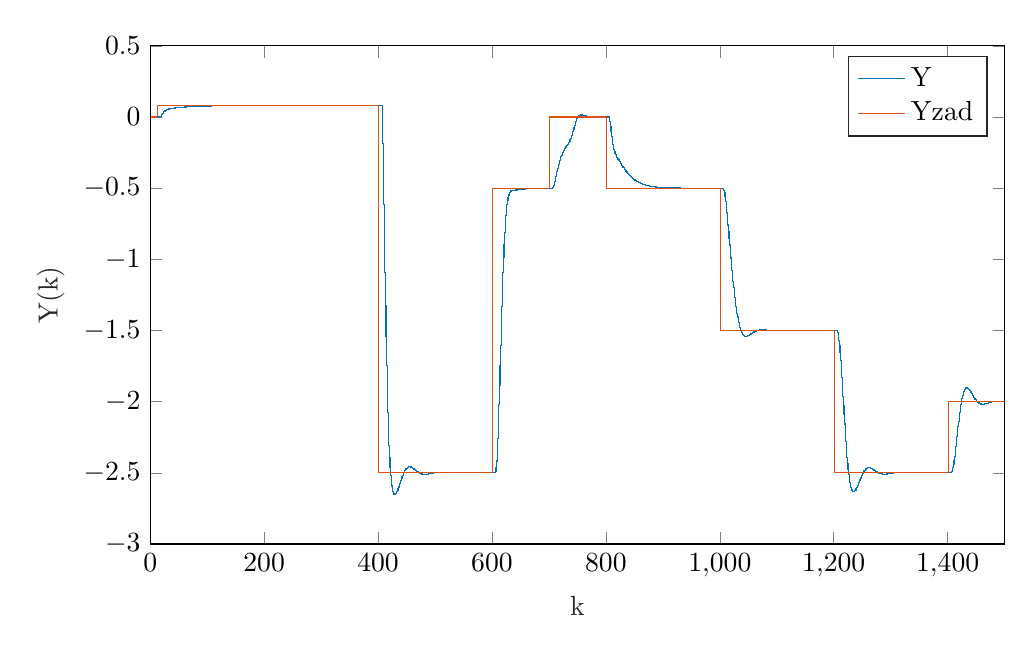
\begin{tikzpicture}

\begin{axis}[%
width=4.272in,
height=2.491in,
at={(0.717in,0.423in)},
scale only axis,
xmin=0,
xmax=1500,
xlabel style={font=\color{white!15!black}},
xlabel={k},
ymin=-3,
ymax=0.5,
ylabel style={font=\color{white!15!black}},
ylabel={Y(k)},
axis background/.style={fill=white},
legend style={legend cell align=left, align=left, draw=white!15!black}
]
\addplot[const plot, color=mycolor1] table[row sep=crcr] {%
1	0\\
2	0\\
3	0\\
4	0\\
5	0\\
6	0\\
7	0\\
8	0\\
9	0\\
10	0\\
11	0\\
12	0\\
13	0\\
14	0\\
15	0\\
16	0\\
17	0.00115627118794366\\
18	0.00442032538565593\\
19	0.00943663872466664\\
20	0.0153996604505715\\
21	0.0215466782921045\\
22	0.0273527439919402\\
23	0.0325417722280601\\
24	0.0370239350682409\\
25	0.0408215731589639\\
26	0.0440109899375717\\
27	0.0466789954337115\\
28	0.0488974914407404\\
29	0.0507441920446542\\
30	0.0522958634740927\\
31	0.0536199201180448\\
32	0.0547706526893509\\
33	0.0557894541953402\\
34	0.0567070891245877\\
35	0.0575461727771125\\
36	0.0583232329420611\\
37	0.0590503054117297\\
38	0.0597361514055664\\
39	0.0603871780042758\\
40	0.0610081209504171\\
41	0.0616025380377963\\
42	0.062173156968323\\
43	0.0627221163187887\\
44	0.063251131051338\\
45	0.0637616062595965\\
46	0.0642547159907358\\
47	0.0647314586438548\\
48	0.0651926966095746\\
49	0.0656391851976115\\
50	0.0660715941661429\\
51	0.0664905240398535\\
52	0.0668965186769851\\
53	0.0672900750778231\\
54	0.067671651123903\\
55	0.0680416717382258\\
56	0.0684005338236317\\
57	0.0687486102451965\\
58	0.0690862530582306\\
59	0.0694137961370214\\
60	0.0697315573251202\\
61	0.0700398402020858\\
62	0.0703389355417711\\
63	0.070629122521868\\
64	0.0709106697323968\\
65	0.0711838360213451\\
66	0.0714488712081479\\
67	0.071706016689716\\
68	0.0719555059589414\\
69	0.072197565051777\\
70	0.0724324129359113\\
71	0.0726602618515806\\
72	0.0728813176130633\\
73	0.073095779877788\\
74	0.0733038423886793\\
75	0.0735056931943096\\
76	0.0737015148505686\\
77	0.0738914846068674\\
78	0.0740757745793285\\
79	0.0742545519129586\\
80	0.0744279789344266\\
81	0.0745962132967698\\
82	0.0747594081171041\\
83	0.0749177121082173\\
84	0.0750712697047624\\
85	0.0752202211846359\\
86	0.0753647027860221\\
87	0.0755048468204958\\
88	0.0756407817825096\\
89	0.075772632455532\\
90	0.0759005200150599\\
91	0.076024562128691\\
92	0.0761448730534124\\
93	0.0762615637302382\\
94	0.076374741876309\\
95	0.076484512074552\\
96	0.0765909758609871\\
97	0.0766942318097546\\
98	0.0767943756159332\\
99	0.0768915001762099\\
100	0.0769856956674585\\
101	0.0770770496232794\\
102	0.07716564700855\\
103	0.0772515702920341\\
104	0.077334899517093\\
105	0.0774157123705435\\
106	0.077494084249704\\
107	0.0775700883276693\\
108	0.0776437956168538\\
109	0.0777152750308428\\
110	0.0777845934445897\\
111	0.0778518157529961\\
112	0.0779170049279131\\
113	0.0779802220735993\\
114	0.0780415264806714\\
115	0.0781009756785836\\
116	0.0781586254866692\\
117	0.0782145300637808\\
118	0.0782687419565605\\
119	0.0783213121463753\\
120	0.0783722900949498\\
121	0.0784217237887277\\
122	0.0784696597819952\\
123	0.0785161432387959\\
124	0.0785612179736692\\
125	0.078604926491241\\
126	0.0786473100246966\\
127	0.0786884085731652\\
128	0.0787282609380428\\
129	0.0787669047582836\\
130	0.0788043765446841\\
131	0.0788407117131894\\
132	0.0788759446172455\\
133	0.0789101085792238\\
134	0.078943235920944\\
135	0.0789753579933169\\
136	0.0790065052051334\\
137	0.0790367070510224\\
138	0.0790659921385984\\
139	0.0790943882148243\\
140	0.0791219221916079\\
141	0.0791486201706551\\
142	0.0791745074675992\\
143	0.0791996086354275\\
144	0.0792239474872242\\
145	0.0792475471182482\\
146	0.0792704299273657\\
147	0.0792926176378539\\
148	0.079314131317596\\
149	0.0793349913986818\\
150	0.0793552176964335\\
151	0.0793748294278705\\
152	0.079393845229631\\
153	0.0794122831753653\\
154	0.0794301607926155\\
155	0.0794474950791961\\
156	0.0794643025190915\\
157	0.0794805990978821\\
158	0.0794964003177136\\
159	0.0795117212118229\\
160	0.0795265763586328\\
161	0.0795409798954285\\
162	0.0795549455316274\\
163	0.0795684865616549\\
164	0.0795816158774364\\
165	0.0795943459805175\\
166	0.0796066889938241\\
167	0.0796186566730703\\
168	0.0796302604178271\\
169	0.07964151128226\\
170	0.0796524199855469\\
171	0.0796629969219833\\
172	0.0796732521707863\\
173	0.079683195505605\\
174	0.0796928364037465\\
175	0.0797021840551247\\
176	0.0797112473709422\\
177	0.079720034992111\\
178	0.0797285552974211\\
179	0.0797368164114636\\
180	0.0797448262123167\\
181	0.0797525923390001\\
182	0.0797601221987057\\
183	0.0797674229738115\\
184	0.0797745016286834\\
185	0.0797813649162738\\
186	0.0797880193845209\\
187	0.0797944713825552\\
188	0.0798007270667198\\
189	0.0798067924064087\\
190	0.0798126731897298\\
191	0.0798183750289964\\
192	0.0798239033660542\\
193	0.0798292634774468\\
194	0.0798344604794257\\
195	0.079839499332809\\
196	0.0798443848476938\\
197	0.079849121688026\\
198	0.0798537143760318\\
199	0.0798581672965164\\
200	0.0798624847010315\\
201	0.079866670711918\\
202	0.0798707293262257\\
203	0.0798746644195147\\
204	0.0798784797495425\\
205	0.0798821789598383\\
206	0.0798857655831706\\
207	0.0798892430449085\\
208	0.0798926146662825\\
209	0.0798958836675459\\
210	0.0798990531710402\\
211	0.0799021262041689\\
212	0.0799051057022799\\
213	0.0799079945114613\\
214	0.0799107953912523\\
215	0.0799135110172723\\
216	0.0799161439837696\\
217	0.0799186968060936\\
218	0.0799211719230919\\
219	0.0799235716994342\\
220	0.0799258984278664\\
221	0.0799281543313961\\
222	0.0799303415654116\\
223	0.0799324622197371\\
224	0.0799345183206252\\
225	0.0799365118326888\\
226	0.0799384446607751\\
227	0.0799403186517817\\
228	0.0799421355964186\\
229	0.0799438972309161\\
230	0.0799456052386811\\
231	0.0799472612519027\\
232	0.0799488668531101\\
233	0.0799504235766818\\
234	0.0799519329103099\\
235	0.07995339629642\\
236	0.0799548151335475\\
237	0.0799561907776721\\
238	0.079957524543512\\
239	0.0799588177057792\\
240	0.0799600715003957\\
241	0.0799612871256734\\
242	0.0799624657434581\\
243	0.0799636084802387\\
244	0.0799647164282224\\
245	0.0799657906463776\\
246	0.0799668321614453\\
247	0.0799678419689188\\
248	0.079968821033995\\
249	0.0799697702924953\\
250	0.07997069065176\\
251	0.0799715829915143\\
252	0.0799724481647085\\
253	0.0799732869983326\\
254	0.0799741002942066\\
255	0.0799748888297457\\
256	0.0799756533587029\\
257	0.0799763946118894\\
258	0.0799771132978724\\
259	0.0799778101036519\\
260	0.079978485695317\\
261	0.0799791407186823\\
262	0.0799797757999046\\
263	0.0799803915460814\\
264	0.0799809885458308\\
265	0.0799815673698536\\
266	0.0799821285714789\\
267	0.0799826726871926\\
268	0.07998320023715\\
269	0.0799837117256729\\
270	0.079984207641731\\
271	0.07998468845941\\
272	0.0799851546383635\\
273	0.0799856066242533\\
274	0.0799860448491746\\
275	0.0799864697320688\\
276	0.0799868816791245\\
277	0.079987281084165\\
278	0.079987668329025\\
279	0.0799880437839152\\
280	0.0799884078077767\\
281	0.0799887607486232\\
282	0.0799891029438742\\
283	0.0799894347206773\\
284	0.079989756396221\\
285	0.0799900682780373\\
286	0.0799903706642963\\
287	0.079990663844091\\
288	0.079990948097713\\
289	0.0799912236969215\\
290	0.0799914909052019\\
291	0.0799917499780185\\
292	0.0799920011630583\\
293	0.0799922447004677\\
294	0.0799924808230821\\
295	0.0799927097566485\\
296	0.0799929317200413\\
297	0.0799931469254715\\
298	0.0799933555786894\\
299	0.0799935578791815\\
300	0.0799937540203608\\
301	0.0799939441897523\\
302	0.0799941285691716\\
303	0.0799943073348992\\
304	0.0799944806578488\\
305	0.0799946487037304\\
306	0.0799948116332093\\
307	0.0799949696020592\\
308	0.0799951227613113\\
309	0.0799952712573988\\
310	0.0799954152322965\\
311	0.079995554823657\\
312	0.0799956901649417\\
313	0.0799958213855491\\
314	0.079995948610938\\
315	0.0799960719627474\\
316	0.0799961915589132\\
317	0.0799963075137806\\
318	0.0799964199382134\\
319	0.0799965289397002\\
320	0.079996634622457\\
321	0.079996737087527\\
322	0.0799968364328768\\
323	0.0799969327534907\\
324	0.079997026141461\\
325	0.0799971166860759\\
326	0.0799972044739055\\
327	0.079997289588884\\
328	0.0799973721123903\\
329	0.0799974521233255\\
330	0.0799975296981887\\
331	0.0799976049111495\\
332	0.0799976778341198\\
333	0.0799977485368218\\
334	0.079997817086855\\
335	0.0799978835497606\\
336	0.0799979479890846\\
337	0.0799980104664382\\
338	0.0799980710415566\\
339	0.0799981297723565\\
340	0.079998186714991\\
341	0.0799982419239038\\
342	0.079998295451881\\
343	0.0799983473501013\\
344	0.0799983976681854\\
345	0.0799984464542432\\
346	0.0799984937549198\\
347	0.0799985396154402\\
348	0.0799985840796523\\
349	0.0799986271900692\\
350	0.0799986689879094\\
351	0.0799987095131366\\
352	0.0799987488044978\\
353	0.0799987868995601\\
354	0.0799988238347469\\
355	0.0799988596453728\\
356	0.0799988943656768\\
357	0.0799989280288559\\
358	0.079998960667096\\
359	0.0799989923116032\\
360	0.0799990229926335\\
361	0.0799990527395218\\
362	0.0799990815807096\\
363	0.0799991095437726\\
364	0.0799991366554469\\
365	0.0799991629416546\\
366	0.0799991884275286\\
367	0.0799992131374364\\
368	0.0799992370950039\\
369	0.0799992603231372\\
370	0.0799992828440455\\
371	0.0799993046792615\\
372	0.0799993258496624\\
373	0.0799993463754897\\
374	0.0799993662763686\\
375	0.0799993855713269\\
376	0.0799994042788129\\
377	0.0799994224167133\\
378	0.0799994400023704\\
379	0.079999457052598\\
380	0.0799994735836984\\
381	0.0799994896114774\\
382	0.0799995051512595\\
383	0.0799995202179029\\
384	0.0799995348258129\\
385	0.0799995489889568\\
386	0.0799995627208761\\
387	0.0799995760347004\\
388	0.0799995889431594\\
389	0.0799996014585952\\
390	0.0799996135929741\\
391	0.0799996253578981\\
392	0.079999636764616\\
393	0.0799996478240341\\
394	0.0799996585467266\\
395	0.0799996689429458\\
396	0.0799996790226316\\
397	0.0799996887954217\\
398	0.07999969827066\\
399	0.0799997074574061\\
400	0.0799997163644437\\
401	0.0799997250002891\\
402	0.0799997333731992\\
403	0.0799997414911796\\
404	0.0799997493619921\\
405	0.0799997569931622\\
406	0.077768062057534\\
407	-0.0221085039853576\\
408	-0.185733997030394\\
409	-0.388783396816526\\
410	-0.614220180151273\\
411	-0.850444933957159\\
412	-1.08958794482109\\
413	-1.32395856724066\\
414	-1.54458949194262\\
415	-1.74494891854783\\
416	-1.92180458089783\\
417	-2.07424641130032\\
418	-2.20292885555451\\
419	-2.30949553920105\\
420	-2.39615257209811\\
421	-2.46536084808812\\
422	-2.51962187365079\\
423	-2.5613356930619\\
424	-2.59271321098262\\
425	-2.61572573390054\\
426	-2.6319322120859\\
427	-2.64253074028442\\
428	-2.64846693512253\\
429	-2.65050826736379\\
430	-2.64929392722019\\
431	-2.64536824568337\\
432	-2.63920366379302\\
433	-2.63121683453168\\
434	-2.62177997591754\\
435	-2.61122880488005\\
436	-2.59986793369514\\
437	-2.58797436787388\\
438	-2.5757996082414\\
439	-2.56357077443543\\
440	-2.55149110609813\\
441	-2.53974013965678\\
442	-2.52847379485176\\
443	-2.51782454041863\\
444	-2.50790174843051\\
445	-2.4987922958062\\
446	-2.49056143206164\\
447	-2.48325390102371\\
448	-2.47689528710745\\
449	-2.47149354612446\\
450	-2.46704067533409\\
451	-2.46351447669311\\
452	-2.46088036964648\\
453	-2.45909321418943\\
454	-2.45809911012777\\
455	-2.45783714377762\\
456	-2.45824105844728\\
457	-2.45924082978089\\
458	-2.46076413135983\\
459	-2.46273767984284\\
460	-2.46508845238388\\
461	-2.46774477211056\\
462	-2.47063726009101\\
463	-2.47369965448043\\
464	-2.47686949944167\\
465	-2.48008870800342\\
466	-2.48330400428655\\
467	-2.48646725153053\\
468	-2.48953567312149\\
469	-2.49247197439897\\
470	-2.49524437343036\\
471	-2.49782654921878\\
472	-2.50019751597375\\
473	-2.50234143214122\\
474	-2.50424735287285\\
475	-2.50590893452366\\
476	-2.50732409960615\\
477	-2.50849467040361\\
478	-2.50942597915638\\
479	-2.5101264623862\\
480	-2.51060724651715\\
481	-2.51088173149099\\
482	-2.51096517856474\\
483	-2.510874307924\\
484	-2.51062691115511\\
485	-2.51024148299895\\
486	-2.50973687617017\\
487	-2.50913198237514\\
488	-2.50844544201187\\
489	-2.50769538439402\\
490	-2.50689919971944\\
491	-2.50607334341016\\
492	-2.50523317289371\\
493	-2.50439281638195\\
494	-2.50356507274016\\
495	-2.50276134112838\\
496	-2.50199157874508\\
497	-2.50126428470861\\
498	-2.50058650787757\\
499	-2.49996387623451\\
500	-2.49940064533716\\
501	-2.49889976327395\\
502	-2.49846294954279\\
503	-2.49809078529838\\
504	-2.49778281247997\\
505	-2.49753763943202\\
506	-2.49735305076044\\
507	-2.49722611932072\\
508	-2.49715331840655\\
509	-2.4971306323937\\
510	-2.49715366428906\\
511	-2.49721773883442\\
512	-2.49731800001585\\
513	-2.49744950202786\\
514	-2.49760729293488\\
515	-2.49778649045806\\
516	-2.49798234949113\\
517	-2.49819032111292\\
518	-2.49840610301573\\
519	-2.49862568140595\\
520	-2.49884536455674\\
521	-2.49906180830069\\
522	-2.49927203384414\\
523	-2.49947343836343\\
524	-2.49966379890786\\
525	-2.49984127018452\\
526	-2.50000437683724\\
527	-2.50015200085653\\
528	-2.50028336477021\\
529	-2.5003980112663\\
530	-2.50049577989206\\
531	-2.50057678145639\\
532	-2.50064137073852\\
533	-2.5006901180745\\
534	-2.50072378035695\\
535	-2.50074327194151\\
536	-2.50074963590927\\
537	-2.50074401608666\\
538	-2.50072763017536\\
539	-2.50070174429512\\
540	-2.50066764919252\\
541	-2.50062663831975\\
542	-2.50057998794011\\
543	-2.50052893937149\\
544	-2.50047468343594\\
545	-2.50041834714399\\
546	-2.50036098260514\\
547	-2.50030355812345\\
548	-2.50024695140725\\
549	-2.50019194479687\\
550	-2.50013922239247\\
551	-2.50008936894616\\
552	-2.5000428703686\\
553	-2.50000011568994\\
554	-2.49996140030766\\
555	-2.49992693035036\\
556	-2.49989682798552\\
557	-2.49987113750131\\
558	-2.49984983199668\\
559	-2.49983282052042\\
560	-2.49981995550829\\
561	-2.49981104037684\\
562	-2.49980583714373\\
563	-2.49980407395616\\
564	-2.49980545242181\\
565	-2.49980965464951\\
566	-2.49981634992016\\
567	-2.4998252009216\\
568	-2.49983586949396\\
569	-2.49984802184455\\
570	-2.49986133320332\\
571	-2.49987549190111\\
572	-2.49989020286338\\
573	-2.49990519052168\\
574	-2.49992020115367\\
575	-2.49993500467028\\
576	-2.4999493958752\\
577	-2.49996319522731\\
578	-2.49997624914164\\
579	-2.49998842986784\\
580	-2.49999963498792\\
581	-2.50000978657692\\
582	-2.5000188300711\\
583	-2.50002673288839\\
584	-2.50003348284559\\
585	-2.50003908641542\\
586	-2.50004356686506\\
587	-2.50004696231568\\
588	-2.50004932375977\\
589	-2.50005071307047\\
590	-2.5000512010338\\
591	-2.50005086543155\\
592	-2.50004978919906\\
593	-2.50004805867896\\
594	-2.50004576198803\\
595	-2.50004298751165\\
596	-2.5000398225363\\
597	-2.50003635202808\\
598	-2.50003265756181\\
599	-2.50002881640294\\
600	-2.50002490074159\\
601	-2.50002097707603\\
602	-2.50001710574096\\
603	-2.50001334057385\\
604	-2.50000972871155\\
605	-2.50000631050783\\
606	-2.49102795960179\\
607	-2.46481427877953\\
608	-2.41722640300964\\
609	-2.34725952829524\\
610	-2.2561949311968\\
611	-2.14685694693671\\
612	-2.02299898178462\\
613	-1.88883018242508\\
614	-1.74866673473817\\
615	-1.60667901128801\\
616	-1.46670548831931\\
617	-1.33211214306041\\
618	-1.20568694533365\\
619	-1.0895686078301\\
620	-0.985213927650476\\
621	-0.893407863755322\\
622	-0.814316070110911\\
623	-0.747573441015433\\
624	-0.692397003176049\\
625	-0.647708987374746\\
626	-0.612258611934287\\
627	-0.584726096302234\\
628	-0.56380667370223\\
629	-0.548273312456224\\
630	-0.537018272901009\\
631	-0.529075950423374\\
632	-0.52363061405857\\
633	-0.520012944181314\\
634	-0.517689013943333\\
635	-0.516244805371895\\
636	-0.515368691434435\\
637	-0.514833668308045\\
638	-0.514480550572866\\
639	-0.514202871903722\\
640	-0.513933868770487\\
641	-0.513635656635607\\
642	-0.513290523737384\\
643	-0.512894151576197\\
644	-0.512450508665089\\
645	-0.511968141178959\\
646	-0.511457588332791\\
647	-0.510929674327722\\
648	-0.510394459187601\\
649	-0.509860666543637\\
650	-0.50933544247315\\
651	-0.508824332400727\\
652	-0.508331391525562\\
653	-0.507859367787954\\
654	-0.507409915149767\\
655	-0.506983809405125\\
656	-0.506581149490747\\
657	-0.506201535002851\\
658	-0.505844215985572\\
659	-0.505508214594182\\
660	-0.505192420423073\\
661	-0.504895662500711\\
662	-0.504616761486514\\
663	-0.504354565683257\\
664	-0.5041079742714\\
665	-0.503875950801445\\
666	-0.503657529534317\\
667	-0.50345181675687\\
668	-0.503257988759494\\
669	-0.503075287767742\\
670	-0.502903016780979\\
671	-0.50274053399169\\
672	-0.502587247237085\\
673	-0.502442608764494\\
674	-0.502306110466494\\
675	-0.502177279652909\\
676	-0.502055675367236\\
677	-0.501940885217736\\
678	-0.501832522672541\\
679	-0.50173022475882\\
680	-0.501633650104462\\
681	-0.501542477264019\\
682	-0.50145640327665\\
683	-0.501375142411024\\
684	-0.501298425059611\\
685	-0.501225996751859\\
686	-0.501157617262097\\
687	-0.501093059793439\\
688	-0.50103211022347\\
689	-0.500974566401144\\
690	-0.500920237487107\\
691	-0.500868943331875\\
692	-0.500820513887793\\
693	-0.500774788651932\\
694	-0.500731616137765\\
695	-0.500690853374051\\
696	-0.500652365429637\\
697	-0.500616024963092\\
698	-0.500581711796186\\
699	-0.500549312510258\\
700	-0.500518720064551\\
701	-0.500489833435565\\
702	-0.500462557276483\\
703	-0.50043680159573\\
704	-0.500412481453706\\
705	-0.500389516676766\\
706	-0.498346636935352\\
707	-0.49276375008639\\
708	-0.483274503965158\\
709	-0.470245900110167\\
710	-0.454443218977896\\
711	-0.436776985511759\\
712	-0.418130845203808\\
713	-0.399261501812593\\
714	-0.38075488866888\\
715	-0.363021230412998\\
716	-0.346313476106886\\
717	-0.330756965474926\\
718	-0.31638188397994\\
719	-0.303153346293399\\
720	-0.290996503914802\\
721	-0.279815849169248\\
722	-0.269508979187689\\
723	-0.259975645964952\\
724	-0.251123116129533\\
725	-0.242868838857347\\
726	-0.235141692476435\\
727	-0.22788128449208\\
728	-0.22103664534031\\
729	-0.214564934246927\\
730	-0.208430204263631\\
731	-0.202585430492355\\
732	-0.196876466040422\\
733	-0.19106826940934\\
734	-0.184903202321863\\
735	-0.178136151360533\\
736	-0.170553661579181\\
737	-0.161984279984099\\
738	-0.152306247096397\\
739	-0.141456581093552\\
740	-0.129443170451033\\
741	-0.116358902129216\\
742	-0.102394188298757\\
743	-0.0878419517268732\\
744	-0.0730881753536337\\
745	-0.0585829129600415\\
746	-0.0447921199253599\\
747	-0.0321387255387913\\
748	-0.0209481559643501\\
749	-0.0114141494691265\\
750	-0.00359341193449224\\
751	0.00257370445374119\\
752	0.00722791789129845\\
753	0.0105541779953532\\
754	0.012752100312435\\
755	0.0140165984063556\\
756	0.0145274347742849\\
757	0.0144448350701296\\
758	0.0139085428445834\\
759	0.0130385659693698\\
760	0.0119366529041122\\
761	0.0106880224235403\\
762	0.00936311397861423\\
763	0.00801924259329589\\
764	0.00670210749761153\\
765	0.00544714677647679\\
766	0.00428075701440812\\
767	0.00322140826207623\\
768	0.00228068379595459\\
769	0.00146426612275237\\
770	0.000772880310962863\\
771	0.000203196294311147\\
772	-0.000251315122170763\\
773	-0.000599581843996904\\
774	-0.000852196368068021\\
775	-0.00102075804393926\\
776	-0.00111729971321451\\
777	-0.00115380374224327\\
778	-0.00114180906966913\\
779	-0.00109210749549261\\
780	-0.00101452436504968\\
781	-0.000917776277550691\\
782	-0.000809396605391328\\
783	-0.000695718488058981\\
784	-0.000581904529094258\\
785	-0.000472012587972976\\
786	-0.000369087700252657\\
787	-0.000275271145598063\\
788	-0.000191918884427519\\
789	-0.000119722884478138\\
790	-5.8830164115318e-05\\
791	-8.95561863580368e-06\\
792	3.05141792162072e-05\\
793	6.04280310951774e-05\\
794	8.17890164140572e-05\\
795	9.56855734835202e-05\\
796	0.000103234557634226\\
797	0.000105535680334999\\
798	0.000103636453357818\\
799	9.85065798387594e-05\\
800	9.10206326079799e-05\\
801	8.19478235837943e-05\\
802	7.19476821326376e-05\\
803	6.15705126460831e-05\\
804	5.12615815022982e-05\\
805	4.13680820564969e-05\\
806	-0.0085824235665081\\
807	-0.0319295764930988\\
808	-0.0649797116817783\\
809	-0.101062829280909\\
810	-0.135455342239687\\
811	-0.165868851429341\\
812	-0.191620631430054\\
813	-0.2128857537091\\
814	-0.23023550419027\\
815	-0.24437600668946\\
816	-0.256010175488\\
817	-0.265770384862967\\
818	-0.274190301754947\\
819	-0.281698087908765\\
820	-0.288621194784722\\
821	-0.295197316651059\\
822	-0.301588305938353\\
823	-0.307895014111501\\
824	-0.31417168475706\\
825	-0.320438981485597\\
826	-0.326694650955866\\
827	-0.332922845861729\\
828	-0.339101266686263\\
829	-0.345206012652641\\
830	-0.351214602431548\\
831	-0.357107618688727\\
832	-0.362869381404157\\
833	-0.368487977704789\\
834	-0.373954908719907\\
835	-0.379264552934281\\
836	-0.384413585869691\\
837	-0.389400442007868\\
838	-0.394224861751486\\
839	-0.398887535915045\\
840	-0.403389841776519\\
841	-0.407733655597014\\
842	-0.41192122383179\\
843	-0.415955076402132\\
844	-0.419837968364528\\
845	-0.423572839753661\\
846	-0.427162786635631\\
847	-0.430611038505481\\
848	-0.433920939341785\\
849	-0.437095930861752\\
850	-0.44013953713722\\
851	-0.443055350095888\\
852	-0.445847015642096\\
853	-0.448518220257488\\
854	-0.451072678019692\\
855	-0.453514118028842\\
856	-0.455846272269741\\
857	-0.458072863965657\\
858	-0.460197596497989\\
859	-0.462224142973398\\
860	-0.464156136516752\\
861	-0.465997161356256\\
862	-0.467750744749198\\
863	-0.469420349775955\\
864	-0.471009369009\\
865	-0.472521119044758\\
866	-0.473958835870415\\
867	-0.475325671025889\\
868	-0.476624688512864\\
869	-0.477858862397641\\
870	-0.47903107505218\\
871	-0.480144115977297\\
872	-0.481200681152968\\
873	-0.482203372862663\\
874	-0.483154699941076\\
875	-0.484057078397489\\
876	-0.484912832369945\\
877	-0.485724195368444\\
878	-0.486493311768367\\
879	-0.487222238518291\\
880	-0.487912947029228\\
881	-0.488567325215095\\
882	-0.489187179656872\\
883	-0.489774237865482\\
884	-0.490330150620781\\
885	-0.490856494366385\\
886	-0.491354773642141\\
887	-0.491826423538071\\
888	-0.492272812155463\\
889	-0.492695243062484\\
890	-0.493094957733297\\
891	-0.493473137961077\\
892	-0.493830908236685\\
893	-0.494169338085943\\
894	-0.49448944435958\\
895	-0.494792193470884\\
896	-0.495078503577034\\
897	-0.49534924670086\\
898	-0.495605250790521\\
899	-0.495847301715244\\
900	-0.496076145195811\\
901	-0.496292488669016\\
902	-0.496497003085748\\
903	-0.496690324642727\\
904	-0.496873056448282\\
905	-0.497045770122825\\
906	-0.49720900733494\\
907	-0.497363281274198\\
908	-0.497509078061995\\
909	-0.497646858101852\\
910	-0.49777705737071\\
911	-0.497900088652897\\
912	-0.498016342718438\\
913	-0.498126189447505\\
914	-0.498229978902795\\
915	-0.498328042351638\\
916	-0.498420693239693\\
917	-0.498508228118016\\
918	-0.498590927525342\\
919	-0.498669056827349\\
920	-0.498742867014667\\
921	-0.498812595461364\\
922	-0.498878466645599\\
923	-0.498940692834086\\
924	-0.498999474731966\\
925	-0.499055002099663\\
926	-0.499107454338215\\
927	-0.499157001044538\\
928	-0.499203802538051\\
929	-0.499248010359987\\
930	-0.499289767746738\\
931	-0.499329210078443\\
932	-0.499366465304069\\
933	-0.499401654344113\\
934	-0.499434891472045\\
935	-0.499466284675552\\
936	-0.499495935998597\\
937	-0.499523941865269\\
938	-0.499550393386331\\
939	-0.499575376649385\\
940	-0.499598972993454\\
941	-0.499621259268826\\
942	-0.499642308082897\\
943	-0.499662188032749\\
944	-0.499680963925168\\
945	-0.499698696984742\\
946	-0.499715445050688\\
947	-0.499731262762983\\
948	-0.499746201738379\\
949	-0.49976031073684\\
950	-0.4997736358189\\
951	-0.49978622049444\\
952	-0.499798105863336\\
953	-0.499809330748411\\
954	-0.499819931821124\\
955	-0.499829943720356\\
956	-0.499839399164692\\
957	-0.499848329058542\\
958	-0.499856762592432\\
959	-0.499864727337781\\
960	-0.49987224933647\\
961	-0.499879353185479\\
962	-0.499886062116866\\
963	-0.499892398073338\\
964	-0.499898381779656\\
965	-0.499904032810105\\
966	-0.499909369652235\\
967	-0.499914409767089\\
968	-0.499919169646105\\
969	-0.49992366486487\\
970	-0.499927910133905\\
971	-0.499931919346643\\
972	-0.499935705624754\\
973	-0.499939281360959\\
974	-0.499942658259481\\
975	-0.499945847374248\\
976	-0.499948859144987\\
977	-0.499951703431318\\
978	-0.499954389544959\\
979	-0.499956926280144\\
980	-0.499959321942356\\
981	-0.499961584375472\\
982	-0.499963720987397\\
983	-0.499965738774277\\
984	-0.499967644343373\\
985	-0.499969443934664\\
986	-0.499971143441248\\
987	-0.499972748428616\\
988	-0.499974264152857\\
989	-0.499975695577846\\
990	-0.499977047391483\\
991	-0.499978324021031\\
992	-0.4999795296476\\
993	-0.499980668219823\\
994	-0.499981743466788\\
995	-0.499982758910227\\
996	-0.499983717876053\\
997	-0.499984623505239\\
998	-0.499985478764099\\
999	-0.499986286454001\\
1000	-0.499987049220531\\
1001	-0.499987769562159\\
1002	-0.499988449838416\\
1003	-0.499989092277615\\
1004	-0.499989698984154\\
1005	-0.499990271945398\\
1006	-0.503920069505661\\
1007	-0.514715930487983\\
1008	-0.533231553273948\\
1009	-0.559098075617352\\
1010	-0.591310171473119\\
1011	-0.628614208514192\\
1012	-0.669748060106608\\
1013	-0.713571090404579\\
1014	-0.759118666825443\\
1015	-0.805609295787488\\
1016	-0.852425739906209\\
1017	-0.899085125923739\\
1018	-0.94520760428516\\
1019	-0.990488841318029\\
1020	-1.03467856121074\\
1021	-1.07756538844197\\
1022	-1.11896715690065\\
1023	-1.15872540424841\\
1024	-1.19670273073826\\
1025	-1.23278188541056\\
1026	-1.26686468542381\\
1027	-1.29887298450798\\
1028	-1.32874962809359\\
1029	-1.3564585584329\\
1030	-1.38198429408066\\
1031	-1.40533097778509\\
1032	-1.42652115046104\\
1033	-1.44559436448391\\
1034	-1.46260570527964\\
1035	-1.4776242560653\\
1036	-1.49073151950312\\
1037	-1.50201980071227\\
1038	-1.51159055535861\\
1039	-1.51955271082139\\
1040	-1.5260209746101\\
1041	-1.53111415004281\\
1042	-1.53495348339083\\
1043	-1.53766106870961\\
1044	-1.53935833642343\\
1045	-1.54016464974627\\
1046	-1.54019602994468\\
1047	-1.53956402633468\\
1048	-1.53837474304287\\
1049	-1.53672802991429\\
1050	-1.53471684014443\\
1051	-1.53242675286707\\
1052	-1.5299356551129\\
1053	-1.52731357431406\\
1054	-1.52462264988809\\
1055	-1.52191723039337\\
1056	-1.51924408129537\\
1057	-1.51664268749311\\
1058	-1.51414563439154\\
1059	-1.5117790514185\\
1060	-1.50956310241425\\
1061	-1.50751250819881\\
1062	-1.50563708777552\\
1063	-1.50394230598298\\
1064	-1.50242981689124\\
1065	-1.50109799378577\\
1066	-1.49994243813596\\
1067	-1.49895646145576\\
1068	-1.49813153539289\\
1069	-1.49745770670244\\
1070	-1.49692397494965\\
1071	-1.49651863183601\\
1072	-1.49622956194683\\
1073	-1.49604450547914\\
1074	-1.49595128413283\\
1075	-1.49593799184343\\
1076	-1.49599315241364\\
1077	-1.49610584637536\\
1078	-1.49626580959661\\
1079	-1.49646350625188\\
1080	-1.49669017881194\\
1081	-1.49693787769109\\
1082	-1.4971994731278\\
1083	-1.49746865177599\\
1084	-1.4977399003594\\
1085	-1.49800847859562\\
1086	-1.49827038343706\\
1087	-1.49852230650774\\
1088	-1.49876158644187\\
1089	-1.49898615765653\\
1090	-1.49919449691929\\
1091	-1.49938556890401\\
1092	-1.49955877176782\\
1093	-1.49971388362873\\
1094	-1.4998510106797\\
1095	-1.49997053754053\\
1096	-1.5000730803251\\
1097	-1.50015944278818\\
1098	-1.5002305758136\\
1099	-1.50028754041373\\
1100	-1.50033147432938\\
1101	-1.50036356224802\\
1102	-1.5003850095978\\
1103	-1.50039701982293\\
1104	-1.50040077500376\\
1105	-1.50039741965048\\
1106	-1.50038804747272\\
1107	-1.50037369090778\\
1108	-1.50035531317694\\
1109	-1.50033380263148\\
1110	-1.50030996914748\\
1111	-1.50028454232999\\
1112	-1.50025817129235\\
1113	-1.50023142578479\\
1114	-1.50020479845725\\
1115	-1.500178708054\\
1116	-1.50015350335188\\
1117	-1.50012946766923\\
1118	-1.5001068237884\\
1119	-1.50008573915083\\
1120	-1.50006633119976\\
1121	-1.50004867276154\\
1122	-1.50003279737165\\
1123	-1.50001870446627\\
1124	-1.50000636437391\\
1125	-1.49999572305449\\
1126	-1.49998670654521\\
1127	-1.49997922508306\\
1128	-1.49997317688369\\
1129	-1.49996845156501\\
1130	-1.49996493321129\\
1131	-1.49996250308007\\
1132	-1.49996104195983\\
1133	-1.49996043219073\\
1134	-1.49996055936461\\
1135	-1.49996131372338\\
1136	-1.49996259127678\\
1137	-1.49996429466237\\
1138	-1.4999663337714\\
1139	-1.49996862616425\\
1140	-1.49997109729975\\
1141	-1.49997368060158\\
1142	-1.49997631738451\\
1143	-1.49997895666231\\
1144	-1.49998155485758\\
1145	-1.49998407543272\\
1146	-1.49998648845955\\
1147	-1.49998877014358\\
1148	-1.49999090231742\\
1149	-1.49999287191601\\
1150	-1.49999467044504\\
1151	-1.49999629345221\\
1152	-1.49999774000953\\
1153	-1.49999901221357\\
1154	-1.50000011470923\\
1155	-1.50000105424138\\
1156	-1.50000183923756\\
1157	-1.50000247942418\\
1158	-1.50000298547749\\
1159	-1.50000336871001\\
1160	-1.50000364079231\\
1161	-1.50000381350966\\
1162	-1.50000389855232\\
1163	-1.50000390733795\\
1164	-1.50000385086459\\
1165	-1.50000373959182\\
1166	-1.50000358334824\\
1167	-1.5000033912627\\
1168	-1.50000317171709\\
1169	-1.50000293231823\\
1170	-1.50000267988658\\
1171	-1.50000242045945\\
1172	-1.50000215930658\\
1173	-1.50000190095601\\
1174	-1.5000016492283\\
1175	-1.50000140727738\\
1176	-1.50000117763624\\
1177	-1.50000096226627\\
1178	-1.50000076260859\\
1179	-1.50000057963651\\
1180	-1.50000041390793\\
1181	-1.50000026561692\\
1182	-1.50000013464365\\
1183	-1.5000000206023\\
1184	-1.49999992288615\\
1185	-1.49999984070986\\
1186	-1.4999997731484\\
1187	-1.49999971917258\\
1188	-1.49999967768116\\
1189	-1.49999964752941\\
1190	-1.49999962755417\\
1191	-1.4999996165956\\
1192	-1.49999961351571\\
1193	-1.49999961721378\\
1194	-1.49999962663893\\
1195	-1.49999964080007\\
1196	-1.49999965877335\\
1197	-1.49999967970751\\
1198	-1.49999970282718\\
1199	-1.49999972743449\\
1200	-1.49999975290918\\
1201	-1.49999977870743\\
1202	-1.49999980435956\\
1203	-1.49999982946691\\
1204	-1.49999985369799\\
1205	-1.4999998767841\\
1206	-1.50431060363148\\
1207	-1.51650557414955\\
1208	-1.5380727508272\\
1209	-1.56913009386065\\
1210	-1.60895544362303\\
1211	-1.6563734597343\\
1212	-1.71002251229638\\
1213	-1.76852280100074\\
1214	-1.83057022267214\\
1215	-1.89497911002652\\
1216	-1.96069317515405\\
1217	-2.0267793106792\\
1218	-2.09241431069313\\
1219	-2.15687065690389\\
1220	-2.21950452858148\\
1221	-2.27974715396216\\
1222	-2.33709939634691\\
1223	-2.39014646626567\\
1224	-2.43769239451304\\
1225	-2.47920934976285\\
1226	-2.51466082647144\\
1227	-2.54433335025749\\
1228	-2.56870993895549\\
1229	-2.58837733330642\\
1230	-2.60387000200646\\
1231	-2.61562420093107\\
1232	-2.62400700270258\\
1233	-2.62934502470283\\
1234	-2.63194173384953\\
1235	-2.63208679331205\\
1236	-2.63006053066975\\
1237	-2.62613565616697\\
1238	-2.62057750173933\\
1239	-2.61364347967746\\
1240	-2.60558212115802\\
1241	-2.59663187590673\\
1242	-2.58701977448899\\
1243	-2.57696002861809\\
1244	-2.56665264170384\\
1245	-2.55628210348244\\
1246	-2.54601624048275\\
1247	-2.53600528429833\\
1248	-2.52638120481886\\
1249	-2.51725733887672\\
1250	-2.50872832754879\\
1251	-2.50087035848021\\
1252	-2.49374169487449\\
1253	-2.48738346152319\\
1254	-2.48182065078409\\
1255	-2.47706330739794\\
1256	-2.47310785002389\\
1257	-2.4699384887213\\
1258	-2.467528700502\\
1259	-2.46584272883995\\
1260	-2.46483707717941\\
1261	-2.46446197072318\\
1262	-2.46466276492197\\
1263	-2.46538128301678\\
1264	-2.4665570686457\\
1265	-2.46812854288188\\
1266	-2.47003405810046\\
1267	-2.472212843774\\
1268	-2.47460584166807\\
1269	-2.47715642996028\\
1270	-2.47981103755342\\
1271	-2.48251965131781\\
1272	-2.48523622020607\\
1273	-2.48791896116158\\
1274	-2.49053057251956\\
1275	-2.49303836120221\\
1276	-2.4954142904628\\
1277	-2.49763495525765\\
1278	-2.49968149253918\\
1279	-2.50153943388082\\
1280	-2.50319850787741\\
1281	-2.50465239972103\\
1282	-2.5058984752388\\
1283	-2.50693747650037\\
1284	-2.50777319586389\\
1285	-2.50841213503269\\
1286	-2.50886315534578\\
1287	-2.50913712512786\\
1288	-2.50924656948324\\
1289	-2.50920532743959\\
1290	-2.50902822083778\\
1291	-2.50873073883105\\
1292	-2.50832874130721\\
1293	-2.50783818399116\\
1294	-2.50727486742848\\
1295	-2.50665421150373\\
1296	-2.50599105661657\\
1297	-2.50529949213253\\
1298	-2.50459271224998\\
1299	-2.50388289898615\\
1300	-2.50318113158809\\
1301	-2.50249732132218\\
1302	-2.50184017029188\\
1303	-2.50121715267786\\
1304	-2.50063451658915\\
1305	-2.50009730455663\\
1306	-2.49960939059034\\
1307	-2.4991735316565\\
1308	-2.49879143140627\\
1309	-2.49846381400245\\
1310	-2.49819050593799\\
1311	-2.49797052381784\\
1312	-2.49780216617868\\
1313	-2.49768310754451\\
1314	-2.49761049305666\\
1315	-2.49758103216975\\
1316	-2.49759109006629\\
1317	-2.49763677560968\\
1318	-2.49771402482343\\
1319	-2.49781867905173\\
1320	-2.49794655712043\\
1321	-2.49809352097495\\
1322	-2.49825553442198\\
1323	-2.49842871474255\\
1324	-2.49860937707482\\
1325	-2.49879407158373\\
1326	-2.49897961354235\\
1327	-2.49916310654424\\
1328	-2.4993419591489\\
1329	-2.49951389533223\\
1330	-2.4996769591714\\
1331	-2.49982951423969\\
1332	-2.49997023822089\\
1333	-2.5000981132765\\
1334	-2.50021241271243\\
1335	-2.50031268449574\\
1336	-2.50039873216754\\
1337	-2.50047059368596\\
1338	-2.50052851871386\\
1339	-2.50057294484133\\
1340	-2.50060447320284\\
1341	-2.50062384391491\\
1342	-2.50063191172329\\
1343	-2.50062962220837\\
1344	-2.50061798885723\\
1345	-2.5005980712679\\
1346	-2.50057095471002\\
1347	-2.50053773122417\\
1348	-2.50049948240168\\
1349	-2.50045726394827\\
1350	-2.50041209209752\\
1351	-2.50036493190647\\
1352	-2.50031668743353\\
1353	-2.50026819377055\\
1354	-2.50022021087509\\
1355	-2.50017341912689\\
1356	-2.50012841651322\\
1357	-2.50008571733208\\
1358	-2.50004575228973\\
1359	-2.50000886985906\\
1360	-2.49997533875925\\
1361	-2.49994535141284\\
1362	-2.49991902823528\\
1363	-2.49989642261305\\
1364	-2.49987752642947\\
1365	-2.49986227600243\\
1366	-2.49985055830481\\
1367	-2.49984221734627\\
1368	-2.49983706060419\\
1369	-2.49983486540135\\
1370	-2.49983538513848\\
1371	-2.4998383553008\\
1372	-2.49984349916856\\
1373	-2.49985053317291\\
1374	-2.49985917184943\\
1375	-2.49986913235187\\
1376	-2.49988013849945\\
1377	-2.49989192434026\\
1378	-2.49990423722238\\
1379	-2.49991684037276\\
1380	-2.49992951499121\\
1381	-2.49994206187352\\
1382	-2.49995430258373\\
1383	-2.49996608020016\\
1384	-2.49997725966445\\
1385	-2.49998772776558\\
1386	-2.4999973927938\\
1387	-2.50000618390078\\
1388	-2.50001405020365\\
1389	-2.50002095967046\\
1390	-2.50002689782494\\
1391	-2.500031866307\\
1392	-2.50003588132476\\
1393	-2.50003897203151\\
1394	-2.50004117885969\\
1395	-2.50004255184097\\
1396	-2.50004314893934\\
1397	-2.50004303442137\\
1398	-2.50004227728471\\
1399	-2.50004094976332\\
1400	-2.50003912592481\\
1401	-2.50003688037249\\
1402	-2.50003428706193\\
1403	-2.50003141823929\\
1404	-2.50002834350579\\
1405	-2.5000251290109\\
1406	-2.49782607041021\\
1407	-2.4914682158927\\
1408	-2.48000925791985\\
1409	-2.46323761010427\\
1410	-2.44143827018478\\
1411	-2.41520399119547\\
1412	-2.3852918877083\\
1413	-2.35252312929529\\
1414	-2.31771826392548\\
1415	-2.28165899225189\\
1416	-2.24506771091614\\
1417	-2.20859781643234\\
1418	-2.17282981089667\\
1419	-2.13827015304722\\
1420	-2.10535128528024\\
1421	-2.07443226437205\\
1422	-2.0457999778045\\
1423	-2.0196711452331\\
1424	-1.99619530617944\\
1425	-1.97545888665302\\
1426	-1.95749084856533\\
1427	-1.94226824525814\\
1428	-1.92972238197903\\
1429	-1.91974561862342\\
1430	-1.91219838882088\\
1431	-1.90691609435717\\
1432	-1.90371561965857\\
1433	-1.9024012948436\\
1434	-1.90277021045767\\
1435	-1.90461684632408\\
1436	-1.90773701978051\\
1437	-1.91193118658555\\
1438	-1.91700714392767\\
1439	-1.92278219245925\\
1440	-1.92908481597875\\
1441	-1.9357559355602\\
1442	-1.94264979120566\\
1443	-1.9496344995449\\
1444	-1.95659233137324\\
1445	-1.96341974825849\\
1446	-1.97002723310153\\
1447	-1.97633894617678\\
1448	-1.98229223442459\\
1449	-1.98783701875809\\
1450	-1.99293508169016\\
1451	-1.99755927543122\\
1452	-2.00169266873888\\
1453	-2.00532764918309\\
1454	-2.00846499608473\\
1455	-2.01111293814613\\
1456	-2.01328620867065\\
1457	-2.01500511022007\\
1458	-2.01629459954085\\
1459	-2.01718340257069\\
1460	-2.01770316829123\\
1461	-2.0178876691086\\
1462	-2.01777205431574\\
1463	-2.01739216202649\\
1464	-2.01678389378138\\
1465	-2.01598265482814\\
1466	-2.01502286189626\\
1467	-2.01393751913653\\
1468	-2.01275786180614\\
1469	-2.01151306626769\\
1470	-2.01023002395421\\
1471	-2.00893317614687\\
1472	-2.00764440572739\\
1473	-2.00638298151089\\
1474	-2.0051655503378\\
1475	-2.00400617180571\\
1476	-2.00291639034737\\
1477	-2.0019053393022\\
1478	-2.00097987167523\\
1479	-2.00014471241687\\
1480	-1.999402627277\\
1481	-1.99875460357229\\
1482	-1.99820003854428\\
1483	-1.99773693136282\\
1484	-1.99736207523305\\
1485	-1.99707124648221\\
1486	-1.99685938792541\\
1487	-1.99672078422739\\
1488	-1.99664922738347\\
1489	-1.99663817083028\\
1490	-1.99668087106175\\
1491	-1.99677051596343\\
1492	-1.99690033938688\\
1493	-1.99706372176376\\
1494	-1.99725427680561\\
1495	-1.99746592455044\\
1496	-1.99769295120125\\
1497	-1.9979300563563\\
1498	-1.99817238835711\\
1499	-1.99841556857931\\
1500	-1.99865570556682\\
};
\addlegendentry{Y}

\addplot[const plot, color=mycolor2] table[row sep=crcr] {%
1	0\\
2	0\\
3	0\\
4	0\\
5	0\\
6	0\\
7	0\\
8	0\\
9	0\\
10	0\\
11	0\\
12	0.08\\
13	0.08\\
14	0.08\\
15	0.08\\
16	0.08\\
17	0.08\\
18	0.08\\
19	0.08\\
20	0.08\\
21	0.08\\
22	0.08\\
23	0.08\\
24	0.08\\
25	0.08\\
26	0.08\\
27	0.08\\
28	0.08\\
29	0.08\\
30	0.08\\
31	0.08\\
32	0.08\\
33	0.08\\
34	0.08\\
35	0.08\\
36	0.08\\
37	0.08\\
38	0.08\\
39	0.08\\
40	0.08\\
41	0.08\\
42	0.08\\
43	0.08\\
44	0.08\\
45	0.08\\
46	0.08\\
47	0.08\\
48	0.08\\
49	0.08\\
50	0.08\\
51	0.08\\
52	0.08\\
53	0.08\\
54	0.08\\
55	0.08\\
56	0.08\\
57	0.08\\
58	0.08\\
59	0.08\\
60	0.08\\
61	0.08\\
62	0.08\\
63	0.08\\
64	0.08\\
65	0.08\\
66	0.08\\
67	0.08\\
68	0.08\\
69	0.08\\
70	0.08\\
71	0.08\\
72	0.08\\
73	0.08\\
74	0.08\\
75	0.08\\
76	0.08\\
77	0.08\\
78	0.08\\
79	0.08\\
80	0.08\\
81	0.08\\
82	0.08\\
83	0.08\\
84	0.08\\
85	0.08\\
86	0.08\\
87	0.08\\
88	0.08\\
89	0.08\\
90	0.08\\
91	0.08\\
92	0.08\\
93	0.08\\
94	0.08\\
95	0.08\\
96	0.08\\
97	0.08\\
98	0.08\\
99	0.08\\
100	0.08\\
101	0.08\\
102	0.08\\
103	0.08\\
104	0.08\\
105	0.08\\
106	0.08\\
107	0.08\\
108	0.08\\
109	0.08\\
110	0.08\\
111	0.08\\
112	0.08\\
113	0.08\\
114	0.08\\
115	0.08\\
116	0.08\\
117	0.08\\
118	0.08\\
119	0.08\\
120	0.08\\
121	0.08\\
122	0.08\\
123	0.08\\
124	0.08\\
125	0.08\\
126	0.08\\
127	0.08\\
128	0.08\\
129	0.08\\
130	0.08\\
131	0.08\\
132	0.08\\
133	0.08\\
134	0.08\\
135	0.08\\
136	0.08\\
137	0.08\\
138	0.08\\
139	0.08\\
140	0.08\\
141	0.08\\
142	0.08\\
143	0.08\\
144	0.08\\
145	0.08\\
146	0.08\\
147	0.08\\
148	0.08\\
149	0.08\\
150	0.08\\
151	0.08\\
152	0.08\\
153	0.08\\
154	0.08\\
155	0.08\\
156	0.08\\
157	0.08\\
158	0.08\\
159	0.08\\
160	0.08\\
161	0.08\\
162	0.08\\
163	0.08\\
164	0.08\\
165	0.08\\
166	0.08\\
167	0.08\\
168	0.08\\
169	0.08\\
170	0.08\\
171	0.08\\
172	0.08\\
173	0.08\\
174	0.08\\
175	0.08\\
176	0.08\\
177	0.08\\
178	0.08\\
179	0.08\\
180	0.08\\
181	0.08\\
182	0.08\\
183	0.08\\
184	0.08\\
185	0.08\\
186	0.08\\
187	0.08\\
188	0.08\\
189	0.08\\
190	0.08\\
191	0.08\\
192	0.08\\
193	0.08\\
194	0.08\\
195	0.08\\
196	0.08\\
197	0.08\\
198	0.08\\
199	0.08\\
200	0.08\\
201	0.08\\
202	0.08\\
203	0.08\\
204	0.08\\
205	0.08\\
206	0.08\\
207	0.08\\
208	0.08\\
209	0.08\\
210	0.08\\
211	0.08\\
212	0.08\\
213	0.08\\
214	0.08\\
215	0.08\\
216	0.08\\
217	0.08\\
218	0.08\\
219	0.08\\
220	0.08\\
221	0.08\\
222	0.08\\
223	0.08\\
224	0.08\\
225	0.08\\
226	0.08\\
227	0.08\\
228	0.08\\
229	0.08\\
230	0.08\\
231	0.08\\
232	0.08\\
233	0.08\\
234	0.08\\
235	0.08\\
236	0.08\\
237	0.08\\
238	0.08\\
239	0.08\\
240	0.08\\
241	0.08\\
242	0.08\\
243	0.08\\
244	0.08\\
245	0.08\\
246	0.08\\
247	0.08\\
248	0.08\\
249	0.08\\
250	0.08\\
251	0.08\\
252	0.08\\
253	0.08\\
254	0.08\\
255	0.08\\
256	0.08\\
257	0.08\\
258	0.08\\
259	0.08\\
260	0.08\\
261	0.08\\
262	0.08\\
263	0.08\\
264	0.08\\
265	0.08\\
266	0.08\\
267	0.08\\
268	0.08\\
269	0.08\\
270	0.08\\
271	0.08\\
272	0.08\\
273	0.08\\
274	0.08\\
275	0.08\\
276	0.08\\
277	0.08\\
278	0.08\\
279	0.08\\
280	0.08\\
281	0.08\\
282	0.08\\
283	0.08\\
284	0.08\\
285	0.08\\
286	0.08\\
287	0.08\\
288	0.08\\
289	0.08\\
290	0.08\\
291	0.08\\
292	0.08\\
293	0.08\\
294	0.08\\
295	0.08\\
296	0.08\\
297	0.08\\
298	0.08\\
299	0.08\\
300	0.08\\
301	0.08\\
302	0.08\\
303	0.08\\
304	0.08\\
305	0.08\\
306	0.08\\
307	0.08\\
308	0.08\\
309	0.08\\
310	0.08\\
311	0.08\\
312	0.08\\
313	0.08\\
314	0.08\\
315	0.08\\
316	0.08\\
317	0.08\\
318	0.08\\
319	0.08\\
320	0.08\\
321	0.08\\
322	0.08\\
323	0.08\\
324	0.08\\
325	0.08\\
326	0.08\\
327	0.08\\
328	0.08\\
329	0.08\\
330	0.08\\
331	0.08\\
332	0.08\\
333	0.08\\
334	0.08\\
335	0.08\\
336	0.08\\
337	0.08\\
338	0.08\\
339	0.08\\
340	0.08\\
341	0.08\\
342	0.08\\
343	0.08\\
344	0.08\\
345	0.08\\
346	0.08\\
347	0.08\\
348	0.08\\
349	0.08\\
350	0.08\\
351	0.08\\
352	0.08\\
353	0.08\\
354	0.08\\
355	0.08\\
356	0.08\\
357	0.08\\
358	0.08\\
359	0.08\\
360	0.08\\
361	0.08\\
362	0.08\\
363	0.08\\
364	0.08\\
365	0.08\\
366	0.08\\
367	0.08\\
368	0.08\\
369	0.08\\
370	0.08\\
371	0.08\\
372	0.08\\
373	0.08\\
374	0.08\\
375	0.08\\
376	0.08\\
377	0.08\\
378	0.08\\
379	0.08\\
380	0.08\\
381	0.08\\
382	0.08\\
383	0.08\\
384	0.08\\
385	0.08\\
386	0.08\\
387	0.08\\
388	0.08\\
389	0.08\\
390	0.08\\
391	0.08\\
392	0.08\\
393	0.08\\
394	0.08\\
395	0.08\\
396	0.08\\
397	0.08\\
398	0.08\\
399	0.08\\
400	0.08\\
401	-2.5\\
402	-2.5\\
403	-2.5\\
404	-2.5\\
405	-2.5\\
406	-2.5\\
407	-2.5\\
408	-2.5\\
409	-2.5\\
410	-2.5\\
411	-2.5\\
412	-2.5\\
413	-2.5\\
414	-2.5\\
415	-2.5\\
416	-2.5\\
417	-2.5\\
418	-2.5\\
419	-2.5\\
420	-2.5\\
421	-2.5\\
422	-2.5\\
423	-2.5\\
424	-2.5\\
425	-2.5\\
426	-2.5\\
427	-2.5\\
428	-2.5\\
429	-2.5\\
430	-2.5\\
431	-2.5\\
432	-2.5\\
433	-2.5\\
434	-2.5\\
435	-2.5\\
436	-2.5\\
437	-2.5\\
438	-2.5\\
439	-2.5\\
440	-2.5\\
441	-2.5\\
442	-2.5\\
443	-2.5\\
444	-2.5\\
445	-2.5\\
446	-2.5\\
447	-2.5\\
448	-2.5\\
449	-2.5\\
450	-2.5\\
451	-2.5\\
452	-2.5\\
453	-2.5\\
454	-2.5\\
455	-2.5\\
456	-2.5\\
457	-2.5\\
458	-2.5\\
459	-2.5\\
460	-2.5\\
461	-2.5\\
462	-2.5\\
463	-2.5\\
464	-2.5\\
465	-2.5\\
466	-2.5\\
467	-2.5\\
468	-2.5\\
469	-2.5\\
470	-2.5\\
471	-2.5\\
472	-2.5\\
473	-2.5\\
474	-2.5\\
475	-2.5\\
476	-2.5\\
477	-2.5\\
478	-2.5\\
479	-2.5\\
480	-2.5\\
481	-2.5\\
482	-2.5\\
483	-2.5\\
484	-2.5\\
485	-2.5\\
486	-2.5\\
487	-2.5\\
488	-2.5\\
489	-2.5\\
490	-2.5\\
491	-2.5\\
492	-2.5\\
493	-2.5\\
494	-2.5\\
495	-2.5\\
496	-2.5\\
497	-2.5\\
498	-2.5\\
499	-2.5\\
500	-2.5\\
501	-2.5\\
502	-2.5\\
503	-2.5\\
504	-2.5\\
505	-2.5\\
506	-2.5\\
507	-2.5\\
508	-2.5\\
509	-2.5\\
510	-2.5\\
511	-2.5\\
512	-2.5\\
513	-2.5\\
514	-2.5\\
515	-2.5\\
516	-2.5\\
517	-2.5\\
518	-2.5\\
519	-2.5\\
520	-2.5\\
521	-2.5\\
522	-2.5\\
523	-2.5\\
524	-2.5\\
525	-2.5\\
526	-2.5\\
527	-2.5\\
528	-2.5\\
529	-2.5\\
530	-2.5\\
531	-2.5\\
532	-2.5\\
533	-2.5\\
534	-2.5\\
535	-2.5\\
536	-2.5\\
537	-2.5\\
538	-2.5\\
539	-2.5\\
540	-2.5\\
541	-2.5\\
542	-2.5\\
543	-2.5\\
544	-2.5\\
545	-2.5\\
546	-2.5\\
547	-2.5\\
548	-2.5\\
549	-2.5\\
550	-2.5\\
551	-2.5\\
552	-2.5\\
553	-2.5\\
554	-2.5\\
555	-2.5\\
556	-2.5\\
557	-2.5\\
558	-2.5\\
559	-2.5\\
560	-2.5\\
561	-2.5\\
562	-2.5\\
563	-2.5\\
564	-2.5\\
565	-2.5\\
566	-2.5\\
567	-2.5\\
568	-2.5\\
569	-2.5\\
570	-2.5\\
571	-2.5\\
572	-2.5\\
573	-2.5\\
574	-2.5\\
575	-2.5\\
576	-2.5\\
577	-2.5\\
578	-2.5\\
579	-2.5\\
580	-2.5\\
581	-2.5\\
582	-2.5\\
583	-2.5\\
584	-2.5\\
585	-2.5\\
586	-2.5\\
587	-2.5\\
588	-2.5\\
589	-2.5\\
590	-2.5\\
591	-2.5\\
592	-2.5\\
593	-2.5\\
594	-2.5\\
595	-2.5\\
596	-2.5\\
597	-2.5\\
598	-2.5\\
599	-2.5\\
600	-2.5\\
601	-0.5\\
602	-0.5\\
603	-0.5\\
604	-0.5\\
605	-0.5\\
606	-0.5\\
607	-0.5\\
608	-0.5\\
609	-0.5\\
610	-0.5\\
611	-0.5\\
612	-0.5\\
613	-0.5\\
614	-0.5\\
615	-0.5\\
616	-0.5\\
617	-0.5\\
618	-0.5\\
619	-0.5\\
620	-0.5\\
621	-0.5\\
622	-0.5\\
623	-0.5\\
624	-0.5\\
625	-0.5\\
626	-0.5\\
627	-0.5\\
628	-0.5\\
629	-0.5\\
630	-0.5\\
631	-0.5\\
632	-0.5\\
633	-0.5\\
634	-0.5\\
635	-0.5\\
636	-0.5\\
637	-0.5\\
638	-0.5\\
639	-0.5\\
640	-0.5\\
641	-0.5\\
642	-0.5\\
643	-0.5\\
644	-0.5\\
645	-0.5\\
646	-0.5\\
647	-0.5\\
648	-0.5\\
649	-0.5\\
650	-0.5\\
651	-0.5\\
652	-0.5\\
653	-0.5\\
654	-0.5\\
655	-0.5\\
656	-0.5\\
657	-0.5\\
658	-0.5\\
659	-0.5\\
660	-0.5\\
661	-0.5\\
662	-0.5\\
663	-0.5\\
664	-0.5\\
665	-0.5\\
666	-0.5\\
667	-0.5\\
668	-0.5\\
669	-0.5\\
670	-0.5\\
671	-0.5\\
672	-0.5\\
673	-0.5\\
674	-0.5\\
675	-0.5\\
676	-0.5\\
677	-0.5\\
678	-0.5\\
679	-0.5\\
680	-0.5\\
681	-0.5\\
682	-0.5\\
683	-0.5\\
684	-0.5\\
685	-0.5\\
686	-0.5\\
687	-0.5\\
688	-0.5\\
689	-0.5\\
690	-0.5\\
691	-0.5\\
692	-0.5\\
693	-0.5\\
694	-0.5\\
695	-0.5\\
696	-0.5\\
697	-0.5\\
698	-0.5\\
699	-0.5\\
700	-0.5\\
701	0\\
702	0\\
703	0\\
704	0\\
705	0\\
706	0\\
707	0\\
708	0\\
709	0\\
710	0\\
711	0\\
712	0\\
713	0\\
714	0\\
715	0\\
716	0\\
717	0\\
718	0\\
719	0\\
720	0\\
721	0\\
722	0\\
723	0\\
724	0\\
725	0\\
726	0\\
727	0\\
728	0\\
729	0\\
730	0\\
731	0\\
732	0\\
733	0\\
734	0\\
735	0\\
736	0\\
737	0\\
738	0\\
739	0\\
740	0\\
741	0\\
742	0\\
743	0\\
744	0\\
745	0\\
746	0\\
747	0\\
748	0\\
749	0\\
750	0\\
751	0\\
752	0\\
753	0\\
754	0\\
755	0\\
756	0\\
757	0\\
758	0\\
759	0\\
760	0\\
761	0\\
762	0\\
763	0\\
764	0\\
765	0\\
766	0\\
767	0\\
768	0\\
769	0\\
770	0\\
771	0\\
772	0\\
773	0\\
774	0\\
775	0\\
776	0\\
777	0\\
778	0\\
779	0\\
780	0\\
781	0\\
782	0\\
783	0\\
784	0\\
785	0\\
786	0\\
787	0\\
788	0\\
789	0\\
790	0\\
791	0\\
792	0\\
793	0\\
794	0\\
795	0\\
796	0\\
797	0\\
798	0\\
799	0\\
800	0\\
801	-0.5\\
802	-0.5\\
803	-0.5\\
804	-0.5\\
805	-0.5\\
806	-0.5\\
807	-0.5\\
808	-0.5\\
809	-0.5\\
810	-0.5\\
811	-0.5\\
812	-0.5\\
813	-0.5\\
814	-0.5\\
815	-0.5\\
816	-0.5\\
817	-0.5\\
818	-0.5\\
819	-0.5\\
820	-0.5\\
821	-0.5\\
822	-0.5\\
823	-0.5\\
824	-0.5\\
825	-0.5\\
826	-0.5\\
827	-0.5\\
828	-0.5\\
829	-0.5\\
830	-0.5\\
831	-0.5\\
832	-0.5\\
833	-0.5\\
834	-0.5\\
835	-0.5\\
836	-0.5\\
837	-0.5\\
838	-0.5\\
839	-0.5\\
840	-0.5\\
841	-0.5\\
842	-0.5\\
843	-0.5\\
844	-0.5\\
845	-0.5\\
846	-0.5\\
847	-0.5\\
848	-0.5\\
849	-0.5\\
850	-0.5\\
851	-0.5\\
852	-0.5\\
853	-0.5\\
854	-0.5\\
855	-0.5\\
856	-0.5\\
857	-0.5\\
858	-0.5\\
859	-0.5\\
860	-0.5\\
861	-0.5\\
862	-0.5\\
863	-0.5\\
864	-0.5\\
865	-0.5\\
866	-0.5\\
867	-0.5\\
868	-0.5\\
869	-0.5\\
870	-0.5\\
871	-0.5\\
872	-0.5\\
873	-0.5\\
874	-0.5\\
875	-0.5\\
876	-0.5\\
877	-0.5\\
878	-0.5\\
879	-0.5\\
880	-0.5\\
881	-0.5\\
882	-0.5\\
883	-0.5\\
884	-0.5\\
885	-0.5\\
886	-0.5\\
887	-0.5\\
888	-0.5\\
889	-0.5\\
890	-0.5\\
891	-0.5\\
892	-0.5\\
893	-0.5\\
894	-0.5\\
895	-0.5\\
896	-0.5\\
897	-0.5\\
898	-0.5\\
899	-0.5\\
900	-0.5\\
901	-0.5\\
902	-0.5\\
903	-0.5\\
904	-0.5\\
905	-0.5\\
906	-0.5\\
907	-0.5\\
908	-0.5\\
909	-0.5\\
910	-0.5\\
911	-0.5\\
912	-0.5\\
913	-0.5\\
914	-0.5\\
915	-0.5\\
916	-0.5\\
917	-0.5\\
918	-0.5\\
919	-0.5\\
920	-0.5\\
921	-0.5\\
922	-0.5\\
923	-0.5\\
924	-0.5\\
925	-0.5\\
926	-0.5\\
927	-0.5\\
928	-0.5\\
929	-0.5\\
930	-0.5\\
931	-0.5\\
932	-0.5\\
933	-0.5\\
934	-0.5\\
935	-0.5\\
936	-0.5\\
937	-0.5\\
938	-0.5\\
939	-0.5\\
940	-0.5\\
941	-0.5\\
942	-0.5\\
943	-0.5\\
944	-0.5\\
945	-0.5\\
946	-0.5\\
947	-0.5\\
948	-0.5\\
949	-0.5\\
950	-0.5\\
951	-0.5\\
952	-0.5\\
953	-0.5\\
954	-0.5\\
955	-0.5\\
956	-0.5\\
957	-0.5\\
958	-0.5\\
959	-0.5\\
960	-0.5\\
961	-0.5\\
962	-0.5\\
963	-0.5\\
964	-0.5\\
965	-0.5\\
966	-0.5\\
967	-0.5\\
968	-0.5\\
969	-0.5\\
970	-0.5\\
971	-0.5\\
972	-0.5\\
973	-0.5\\
974	-0.5\\
975	-0.5\\
976	-0.5\\
977	-0.5\\
978	-0.5\\
979	-0.5\\
980	-0.5\\
981	-0.5\\
982	-0.5\\
983	-0.5\\
984	-0.5\\
985	-0.5\\
986	-0.5\\
987	-0.5\\
988	-0.5\\
989	-0.5\\
990	-0.5\\
991	-0.5\\
992	-0.5\\
993	-0.5\\
994	-0.5\\
995	-0.5\\
996	-0.5\\
997	-0.5\\
998	-0.5\\
999	-0.5\\
1000	-0.5\\
1001	-1.5\\
1002	-1.5\\
1003	-1.5\\
1004	-1.5\\
1005	-1.5\\
1006	-1.5\\
1007	-1.5\\
1008	-1.5\\
1009	-1.5\\
1010	-1.5\\
1011	-1.5\\
1012	-1.5\\
1013	-1.5\\
1014	-1.5\\
1015	-1.5\\
1016	-1.5\\
1017	-1.5\\
1018	-1.5\\
1019	-1.5\\
1020	-1.5\\
1021	-1.5\\
1022	-1.5\\
1023	-1.5\\
1024	-1.5\\
1025	-1.5\\
1026	-1.5\\
1027	-1.5\\
1028	-1.5\\
1029	-1.5\\
1030	-1.5\\
1031	-1.5\\
1032	-1.5\\
1033	-1.5\\
1034	-1.5\\
1035	-1.5\\
1036	-1.5\\
1037	-1.5\\
1038	-1.5\\
1039	-1.5\\
1040	-1.5\\
1041	-1.5\\
1042	-1.5\\
1043	-1.5\\
1044	-1.5\\
1045	-1.5\\
1046	-1.5\\
1047	-1.5\\
1048	-1.5\\
1049	-1.5\\
1050	-1.5\\
1051	-1.5\\
1052	-1.5\\
1053	-1.5\\
1054	-1.5\\
1055	-1.5\\
1056	-1.5\\
1057	-1.5\\
1058	-1.5\\
1059	-1.5\\
1060	-1.5\\
1061	-1.5\\
1062	-1.5\\
1063	-1.5\\
1064	-1.5\\
1065	-1.5\\
1066	-1.5\\
1067	-1.5\\
1068	-1.5\\
1069	-1.5\\
1070	-1.5\\
1071	-1.5\\
1072	-1.5\\
1073	-1.5\\
1074	-1.5\\
1075	-1.5\\
1076	-1.5\\
1077	-1.5\\
1078	-1.5\\
1079	-1.5\\
1080	-1.5\\
1081	-1.5\\
1082	-1.5\\
1083	-1.5\\
1084	-1.5\\
1085	-1.5\\
1086	-1.5\\
1087	-1.5\\
1088	-1.5\\
1089	-1.5\\
1090	-1.5\\
1091	-1.5\\
1092	-1.5\\
1093	-1.5\\
1094	-1.5\\
1095	-1.5\\
1096	-1.5\\
1097	-1.5\\
1098	-1.5\\
1099	-1.5\\
1100	-1.5\\
1101	-1.5\\
1102	-1.5\\
1103	-1.5\\
1104	-1.5\\
1105	-1.5\\
1106	-1.5\\
1107	-1.5\\
1108	-1.5\\
1109	-1.5\\
1110	-1.5\\
1111	-1.5\\
1112	-1.5\\
1113	-1.5\\
1114	-1.5\\
1115	-1.5\\
1116	-1.5\\
1117	-1.5\\
1118	-1.5\\
1119	-1.5\\
1120	-1.5\\
1121	-1.5\\
1122	-1.5\\
1123	-1.5\\
1124	-1.5\\
1125	-1.5\\
1126	-1.5\\
1127	-1.5\\
1128	-1.5\\
1129	-1.5\\
1130	-1.5\\
1131	-1.5\\
1132	-1.5\\
1133	-1.5\\
1134	-1.5\\
1135	-1.5\\
1136	-1.5\\
1137	-1.5\\
1138	-1.5\\
1139	-1.5\\
1140	-1.5\\
1141	-1.5\\
1142	-1.5\\
1143	-1.5\\
1144	-1.5\\
1145	-1.5\\
1146	-1.5\\
1147	-1.5\\
1148	-1.5\\
1149	-1.5\\
1150	-1.5\\
1151	-1.5\\
1152	-1.5\\
1153	-1.5\\
1154	-1.5\\
1155	-1.5\\
1156	-1.5\\
1157	-1.5\\
1158	-1.5\\
1159	-1.5\\
1160	-1.5\\
1161	-1.5\\
1162	-1.5\\
1163	-1.5\\
1164	-1.5\\
1165	-1.5\\
1166	-1.5\\
1167	-1.5\\
1168	-1.5\\
1169	-1.5\\
1170	-1.5\\
1171	-1.5\\
1172	-1.5\\
1173	-1.5\\
1174	-1.5\\
1175	-1.5\\
1176	-1.5\\
1177	-1.5\\
1178	-1.5\\
1179	-1.5\\
1180	-1.5\\
1181	-1.5\\
1182	-1.5\\
1183	-1.5\\
1184	-1.5\\
1185	-1.5\\
1186	-1.5\\
1187	-1.5\\
1188	-1.5\\
1189	-1.5\\
1190	-1.5\\
1191	-1.5\\
1192	-1.5\\
1193	-1.5\\
1194	-1.5\\
1195	-1.5\\
1196	-1.5\\
1197	-1.5\\
1198	-1.5\\
1199	-1.5\\
1200	-1.5\\
1201	-2.5\\
1202	-2.5\\
1203	-2.5\\
1204	-2.5\\
1205	-2.5\\
1206	-2.5\\
1207	-2.5\\
1208	-2.5\\
1209	-2.5\\
1210	-2.5\\
1211	-2.5\\
1212	-2.5\\
1213	-2.5\\
1214	-2.5\\
1215	-2.5\\
1216	-2.5\\
1217	-2.5\\
1218	-2.5\\
1219	-2.5\\
1220	-2.5\\
1221	-2.5\\
1222	-2.5\\
1223	-2.5\\
1224	-2.5\\
1225	-2.5\\
1226	-2.5\\
1227	-2.5\\
1228	-2.5\\
1229	-2.5\\
1230	-2.5\\
1231	-2.5\\
1232	-2.5\\
1233	-2.5\\
1234	-2.5\\
1235	-2.5\\
1236	-2.5\\
1237	-2.5\\
1238	-2.5\\
1239	-2.5\\
1240	-2.5\\
1241	-2.5\\
1242	-2.5\\
1243	-2.5\\
1244	-2.5\\
1245	-2.5\\
1246	-2.5\\
1247	-2.5\\
1248	-2.5\\
1249	-2.5\\
1250	-2.5\\
1251	-2.5\\
1252	-2.5\\
1253	-2.5\\
1254	-2.5\\
1255	-2.5\\
1256	-2.5\\
1257	-2.5\\
1258	-2.5\\
1259	-2.5\\
1260	-2.5\\
1261	-2.5\\
1262	-2.5\\
1263	-2.5\\
1264	-2.5\\
1265	-2.5\\
1266	-2.5\\
1267	-2.5\\
1268	-2.5\\
1269	-2.5\\
1270	-2.5\\
1271	-2.5\\
1272	-2.5\\
1273	-2.5\\
1274	-2.5\\
1275	-2.5\\
1276	-2.5\\
1277	-2.5\\
1278	-2.5\\
1279	-2.5\\
1280	-2.5\\
1281	-2.5\\
1282	-2.5\\
1283	-2.5\\
1284	-2.5\\
1285	-2.5\\
1286	-2.5\\
1287	-2.5\\
1288	-2.5\\
1289	-2.5\\
1290	-2.5\\
1291	-2.5\\
1292	-2.5\\
1293	-2.5\\
1294	-2.5\\
1295	-2.5\\
1296	-2.5\\
1297	-2.5\\
1298	-2.5\\
1299	-2.5\\
1300	-2.5\\
1301	-2.5\\
1302	-2.5\\
1303	-2.5\\
1304	-2.5\\
1305	-2.5\\
1306	-2.5\\
1307	-2.5\\
1308	-2.5\\
1309	-2.5\\
1310	-2.5\\
1311	-2.5\\
1312	-2.5\\
1313	-2.5\\
1314	-2.5\\
1315	-2.5\\
1316	-2.5\\
1317	-2.5\\
1318	-2.5\\
1319	-2.5\\
1320	-2.5\\
1321	-2.5\\
1322	-2.5\\
1323	-2.5\\
1324	-2.5\\
1325	-2.5\\
1326	-2.5\\
1327	-2.5\\
1328	-2.5\\
1329	-2.5\\
1330	-2.5\\
1331	-2.5\\
1332	-2.5\\
1333	-2.5\\
1334	-2.5\\
1335	-2.5\\
1336	-2.5\\
1337	-2.5\\
1338	-2.5\\
1339	-2.5\\
1340	-2.5\\
1341	-2.5\\
1342	-2.5\\
1343	-2.5\\
1344	-2.5\\
1345	-2.5\\
1346	-2.5\\
1347	-2.5\\
1348	-2.5\\
1349	-2.5\\
1350	-2.5\\
1351	-2.5\\
1352	-2.5\\
1353	-2.5\\
1354	-2.5\\
1355	-2.5\\
1356	-2.5\\
1357	-2.5\\
1358	-2.5\\
1359	-2.5\\
1360	-2.5\\
1361	-2.5\\
1362	-2.5\\
1363	-2.5\\
1364	-2.5\\
1365	-2.5\\
1366	-2.5\\
1367	-2.5\\
1368	-2.5\\
1369	-2.5\\
1370	-2.5\\
1371	-2.5\\
1372	-2.5\\
1373	-2.5\\
1374	-2.5\\
1375	-2.5\\
1376	-2.5\\
1377	-2.5\\
1378	-2.5\\
1379	-2.5\\
1380	-2.5\\
1381	-2.5\\
1382	-2.5\\
1383	-2.5\\
1384	-2.5\\
1385	-2.5\\
1386	-2.5\\
1387	-2.5\\
1388	-2.5\\
1389	-2.5\\
1390	-2.5\\
1391	-2.5\\
1392	-2.5\\
1393	-2.5\\
1394	-2.5\\
1395	-2.5\\
1396	-2.5\\
1397	-2.5\\
1398	-2.5\\
1399	-2.5\\
1400	-2.5\\
1401	-2\\
1402	-2\\
1403	-2\\
1404	-2\\
1405	-2\\
1406	-2\\
1407	-2\\
1408	-2\\
1409	-2\\
1410	-2\\
1411	-2\\
1412	-2\\
1413	-2\\
1414	-2\\
1415	-2\\
1416	-2\\
1417	-2\\
1418	-2\\
1419	-2\\
1420	-2\\
1421	-2\\
1422	-2\\
1423	-2\\
1424	-2\\
1425	-2\\
1426	-2\\
1427	-2\\
1428	-2\\
1429	-2\\
1430	-2\\
1431	-2\\
1432	-2\\
1433	-2\\
1434	-2\\
1435	-2\\
1436	-2\\
1437	-2\\
1438	-2\\
1439	-2\\
1440	-2\\
1441	-2\\
1442	-2\\
1443	-2\\
1444	-2\\
1445	-2\\
1446	-2\\
1447	-2\\
1448	-2\\
1449	-2\\
1450	-2\\
1451	-2\\
1452	-2\\
1453	-2\\
1454	-2\\
1455	-2\\
1456	-2\\
1457	-2\\
1458	-2\\
1459	-2\\
1460	-2\\
1461	-2\\
1462	-2\\
1463	-2\\
1464	-2\\
1465	-2\\
1466	-2\\
1467	-2\\
1468	-2\\
1469	-2\\
1470	-2\\
1471	-2\\
1472	-2\\
1473	-2\\
1474	-2\\
1475	-2\\
1476	-2\\
1477	-2\\
1478	-2\\
1479	-2\\
1480	-2\\
1481	-2\\
1482	-2\\
1483	-2\\
1484	-2\\
1485	-2\\
1486	-2\\
1487	-2\\
1488	-2\\
1489	-2\\
1490	-2\\
1491	-2\\
1492	-2\\
1493	-2\\
1494	-2\\
1495	-2\\
1496	-2\\
1497	-2\\
1498	-2\\
1499	-2\\
1500	-2\\
};
\addlegendentry{Yzad}

\end{axis}
\end{tikzpicture}%
\caption{Regulacja rozmyta DMC, 2 regulatory}
\end{figure}

\begin{figure}[H]
\centering
% This file was created by matlab2tikz.
%
%The latest updates can be retrieved from
%  http://www.mathworks.com/matlabcentral/fileexchange/22022-matlab2tikz-matlab2tikz
%where you can also make suggestions and rate matlab2tikz.
%
\definecolor{mycolor1}{rgb}{0.00000,0.44700,0.74100}%
%
\begin{tikzpicture}

\begin{axis}[%
width=4.272in,
height=2.491in,
at={(0.717in,0.423in)},
scale only axis,
xmin=0,
xmax=1500,
xlabel style={font=\color{white!15!black}},
xlabel={k},
ymin=-1.1,
ymax=1.1,
ylabel style={font=\color{white!15!black}},
ylabel={U(k)},
axis background/.style={fill=white}
]
\addplot[const plot, color=mycolor1, forget plot] table[row sep=crcr] {%
1	0\\
2	0\\
3	0\\
4	0\\
5	0\\
6	0\\
7	0\\
8	0\\
9	0\\
10	0\\
11	0\\
12	0.0244941486179135\\
13	0.0503586642396553\\
14	0.0775517459560946\\
15	0.106042010232295\\
16	0.1358023626412\\
17	0.166430865355841\\
18	0.197271259188669\\
19	0.227540486567625\\
20	0.256587607921706\\
21	0.283687159671608\\
22	0.307834402795637\\
23	0.329458989249588\\
24	0.349002410804788\\
25	0.36685675755133\\
26	0.383341220463532\\
27	0.398706783787198\\
28	0.413155501246113\\
29	0.426844849107033\\
30	0.439893138290003\\
31	0.452387249017562\\
32	0.464390693681126\\
33	0.475950496383093\\
34	0.487102377907887\\
35	0.497874348832693\\
36	0.508289108043425\\
37	0.518365621568237\\
38	0.528120164208526\\
39	0.537567014942538\\
40	0.546718929621712\\
41	0.555587469621883\\
42	0.564183236320159\\
43	0.572516042949828\\
44	0.580595043827536\\
45	0.588428833735628\\
46	0.59602552578492\\
47	0.603392813331322\\
48	0.610538019801349\\
49	0.617468139181142\\
50	0.6241898692009\\
51	0.630709638747495\\
52	0.637033630682233\\
53	0.643167800979552\\
54	0.649117894906062\\
55	0.654889460808957\\
56	0.660487861966221\\
57	0.665918286859722\\
58	0.671185758160354\\
59	0.676295140657407\\
60	0.681251148319047\\
61	0.686058350634664\\
62	0.690721178360931\\
63	0.695243928770259\\
64	0.699630770481688\\
65	0.703885747939249\\
66	0.708012785590736\\
67	0.71201569181005\\
68	0.715898162598345\\
69	0.719663785092826\\
70	0.723316040906831\\
71	0.726858309320642\\
72	0.730293870339014\\
73	0.733625907628673\\
74	0.736857511346743\\
75	0.739991680869257\\
76	0.743031327427387\\
77	0.745979276657837\\
78	0.74883827107285\\
79	0.751610972454467\\
80	0.754299964177029\\
81	0.756907753461394\\
82	0.759436773563879\\
83	0.761889385902599\\
84	0.764267882123592\\
85	0.766574486108859\\
86	0.768811355928283\\
87	0.770980585737196\\
88	0.773084207621266\\
89	0.775124193390248\\
90	0.777102456322035\\
91	0.779020852858416\\
92	0.780881184253821\\
93	0.78268519817834\\
94	0.784434590276194\\
95	0.786131005680848\\
96	0.787776040487878\\
97	0.789371243186697\\
98	0.790918116052198\\
99	0.792418116497349\\
100	0.793872658387766\\
101	0.795283113319222\\
102	0.796650811859083\\
103	0.7979770447526\\
104	0.799263064094968\\
105	0.800510084470071\\
106	0.80171928405677\\
107	0.802891805703614\\
108	0.804028757972797\\
109	0.805131216154189\\
110	0.80620022325025\\
111	0.807236790932595\\
112	0.808241900470996\\
113	0.809216503635552\\
114	0.810161523572769\\
115	0.811077855656257\\
116	0.811966368312751\\
117	0.81282790382412\\
118	0.813663279106039\\
119	0.814473286463976\\
120	0.815258694327105\\
121	0.816020247960785\\
122	0.816758670158187\\
123	0.817474661911661\\
124	0.81816890306442\\
125	0.818842052943078\\
126	0.819494750971606\\
127	0.82012761726721\\
128	0.820741253218672\\
129	0.821336242047618\\
130	0.821913149353242\\
131	0.822472523640919\\
132	0.823014896835197\\
133	0.823540784777605\\
134	0.824050687709715\\
135	0.824545090741887\\
136	0.825024464308097\\
137	0.825489264607272\\
138	0.825939934031507\\
139	0.826376901581543\\
140	0.826800583269892\\
141	0.82721138251195\\
142	0.82760969050546\\
143	0.827995886598658\\
144	0.828370338647442\\
145	0.82873340336187\\
146	0.829085426642314\\
147	0.829426743905565\\
148	0.829757680401189\\
149	0.830078551518414\\
150	0.830389663083836\\
151	0.830691311650199\\
152	0.830983784776533\\
153	0.831267361299889\\
154	0.831542311598919\\
155	0.831808897849558\\
156	0.832067374273021\\
157	0.832317987376355\\
158	0.832560976185768\\
159	0.832796572472939\\
160	0.833025000974529\\
161	0.833246479605086\\
162	0.833461219663541\\
163	0.833669426033499\\
164	0.833871297377488\\
165	0.834067026325362\\
166	0.834256799657028\\
167	0.834440798479666\\
168	0.834619198399602\\
169	0.834792169689004\\
170	0.834959877447543\\
171	0.835122481759182\\
172	0.835280137844231\\
173	0.835432996206807\\
174	0.835581202777847\\
175	0.835724899053798\\
176	0.835864222231121\\
177	0.83599930533672\\
178	0.836130277354444\\
179	0.836257263347752\\
180	0.836380384578671\\
181	0.836499758623164\\
182	0.836615499482998\\
183	0.836727717694232\\
184	0.836836520432422\\
185	0.836942011614638\\
186	0.837044291998403\\
187	0.837143459277617\\
188	0.837239608175599\\
189	0.837332830535293\\
190	0.837423215406748\\
191	0.837510849131951\\
192	0.837595815427085\\
193	0.83767819546229\\
194	0.837758067939018\\
195	0.837835509165032\\
196	0.837910593127136\\
197	0.837983391561699\\
198	0.838053974023042\\
199	0.838122407949745\\
200	0.83818875872895\\
201	0.838253089758709\\
202	0.83831546250844\\
203	0.83837593657755\\
204	0.83843456975228\\
205	0.838491418060822\\
206	0.838546535826766\\
207	0.838599975720921\\
208	0.838651788811565\\
209	0.838702024613173\\
210	0.838750731133656\\
211	0.838797954920176\\
212	0.838843741103561\\
213	0.838888133441378\\
214	0.838931174359694\\
215	0.838972904993567\\
216	0.839013365226311\\
217	0.839052593727569\\
218	0.839090627990218\\
219	0.839127504366173\\
220	0.839163258101081\\
221	0.839197923367976\\
222	0.839231533299907\\
223	0.839264120021571\\
224	0.839295714679988\\
225	0.839326347474245\\
226	0.839356047684332\\
227	0.839384843699102\\
228	0.839412763043386\\
229	0.839439832404276\\
230	0.839466077656618\\
231	0.83949152388772\\
232	0.839516195421315\\
233	0.839540115840795\\
234	0.839563308011739\\
235	0.839585794103751\\
236	0.839607595611641\\
237	0.839628733375954\\
238	0.839649227602884\\
239	0.839669097883574\\
240	0.839688363212835\\
241	0.839707042007289\\
242	0.839725152122968\\
243	0.839742710872374\\
244	0.839759735041017\\
245	0.839776240903454\\
246	0.839792244238842\\
247	0.839807760346011\\
248	0.839822804058084\\
249	0.83983738975665\\
250	0.839851531385508\\
251	0.839865242463991\\
252	0.839878536099882\\
253	0.839891425001943\\
254	0.83990392149206\\
255	0.839916037517017\\
256	0.83992778465991\\
257	0.839939174151225\\
258	0.83995021687956\\
259	0.83996092340204\\
260	0.839971303954404\\
261	0.839981368460783\\
262	0.839991126543192\\
263	0.84000058753072\\
264	0.840009760468453\\
265	0.84001865412611\\
266	0.840027277006434\\
267	0.840035637353313\\
268	0.840043743159662\\
269	0.840051602175062\\
270	0.840059221913168\\
271	0.840066609658887\\
272	0.840073772475349\\
273	0.84008071721065\\
274	0.840087450504403\\
275	0.840093978794081\\
276	0.840100308321176\\
277	0.840106445137157\\
278	0.840112395109262\\
279	0.840118163926104\\
280	0.840123757103105\\
281	0.840129179987774\\
282	0.840134437764815\\
283	0.840139535461086\\
284	0.840144477950401\\
285	0.840149269958191\\
286	0.840153916066023\\
287	0.840158420715975\\
288	0.840162788214886\\
289	0.840167022738475\\
290	0.840171128335325\\
291	0.840175108930764\\
292	0.840178968330608\\
293	0.840182710224805\\
294	0.84018633819096\\
295	0.840189855697758\\
296	0.840193266108275\\
297	0.840196572683198\\
298	0.840199778583939\\
299	0.84020288687566\\
300	0.840205900530202\\
301	0.840208822428925\\
302	0.840211655365463\\
303	0.840214402048398\\
304	0.840217065103844\\
305	0.840219647077962\\
306	0.840222150439394\\
307	0.840224577581619\\
308	0.840226930825246\\
309	0.84022921242023\\
310	0.840231424548024\\
311	0.840233569323665\\
312	0.840235648797793\\
313	0.840237664958617\\
314	0.84023961973381\\
315	0.840241514992356\\
316	0.840243352546335\\
317	0.840245134152657\\
318	0.84024686151474\\
319	0.840248536284138\\
320	0.840250160062123\\
321	0.840251734401214\\
322	0.840253260806661\\
323	0.840254740737884\\
324	0.840256175609869\\
325	0.840257566794522\\
326	0.84025891562198\\
327	0.840260223381878\\
328	0.840261491324591\\
329	0.840262720662422\\
330	0.840263912570763\\
331	0.840265068189222\\
332	0.840266188622706\\
333	0.840267274942487\\
334	0.840268328187214\\
335	0.840269349363918\\
336	0.840270339448966\\
337	0.840271299389001\\
338	0.84027223010184\\
339	0.840273132477359\\
340	0.840274007378338\\
341	0.840274855641291\\
342	0.84027567807726\\
343	0.840276475472595\\
344	0.840277248589703\\
345	0.840277998167781\\
346	0.840278724923517\\
347	0.840279429551779\\
348	0.84028011272628\\
349	0.840280775100219\\
350	0.840281417306908\\
351	0.840282039960376\\
352	0.840282643655957\\
353	0.84028322897086\\
354	0.84028379646472\\
355	0.84028434668013\\
356	0.840284880143167\\
357	0.840285397363887\\
358	0.840285898836819\\
359	0.840286385041434\\
360	0.840286856442604\\
361	0.840287313491049\\
362	0.840287756623765\\
363	0.840288186264442\\
364	0.840288602823871\\
365	0.840289006700336\\
366	0.840289398279995\\
367	0.840289777937245\\
368	0.84029014603509\\
369	0.840290502925475\\
370	0.840290848949635\\
371	0.840291184438412\\
372	0.840291509712576\\
373	0.840291825083131\\
374	0.840292130851612\\
375	0.840292427310371\\
376	0.840292714742862\\
377	0.840292993423906\\
378	0.840293263619959\\
379	0.840293525589362\\
380	0.840293779582592\\
381	0.840294025842499\\
382	0.840294264604538\\
383	0.840294496096997\\
384	0.840294720541213\\
385	0.840294938151782\\
386	0.84029514913677\\
387	0.840295353697903\\
388	0.84029555203077\\
389	0.840295744325001\\
390	0.840295930764455\\
391	0.840296111527393\\
392	0.840296286786646\\
393	0.840296456709785\\
394	0.840296621459279\\
395	0.840296781192649\\
396	0.84029693606262\\
397	0.84029708621727\\
398	0.840297231800165\\
399	0.8402973729505\\
400	0.840297509803235\\
401	-0.680810491001643\\
402	-0.73710842392183\\
403	-0.790773735778304\\
404	-0.841745091787239\\
405	-0.890042922186131\\
406	-0.936060530917494\\
407	-0.978229080001169\\
408	-1\\
409	-1\\
410	-1\\
411	-1\\
412	-1\\
413	-1\\
414	-1\\
415	-1\\
416	-1\\
417	-1\\
418	-1\\
419	-1\\
420	-0.999985185569682\\
421	-0.999150860322002\\
422	-0.997706879668174\\
423	-0.995818701822473\\
424	-0.993614875554899\\
425	-0.99119402333623\\
426	-0.988634241588128\\
427	-0.986000916157387\\
428	-0.983350378464288\\
429	-0.980731827714603\\
430	-0.978188201181807\\
431	-0.97575649020411\\
432	-0.973467838336355\\
433	-0.971347603289063\\
434	-0.969415480891202\\
435	-0.967685751679891\\
436	-0.966167639442183\\
437	-0.964865743172087\\
438	-0.963780508208963\\
439	-0.962908710481817\\
440	-0.96224393654062\\
441	-0.961777052987814\\
442	-0.961496645209944\\
443	-0.96138944584515\\
444	-0.961440739679987\\
445	-0.96163474459323\\
446	-0.961954966997985\\
447	-0.96238453117757\\
448	-0.962906481997203\\
449	-0.963504059288205\\
450	-0.964160942259344\\
451	-0.964861462710951\\
452	-0.96559078644997\\
453	-0.966335063000192\\
454	-0.96708154435835\\
455	-0.967818674102631\\
456	-0.968536148607235\\
457	-0.969224952440168\\
458	-0.969877370228127\\
459	-0.970486977384558\\
460	-0.971048612137205\\
461	-0.971558331277987\\
462	-0.972013352012289\\
463	-0.97241198220065\\
464	-0.972753541195294\\
465	-0.973038273363545\\
466	-0.973267256269135\\
467	-0.973442305352382\\
468	-0.973565876813188\\
469	-0.973640970258854\\
470	-0.973671032532581\\
471	-0.973659863989684\\
472	-0.973611528338302\\
473	-0.973530267011157\\
474	-0.973420418885963\\
475	-0.973286346025743\\
476	-0.97313236596777\\
477	-0.972962690952206\\
478	-0.972781374349915\\
479	-0.972592264424384\\
480	-0.972398965446139\\
481	-0.972204806070373\\
482	-0.972012814790566\\
483	-0.971825702193226\\
484	-0.971645849662152\\
485	-0.971475304115144\\
486	-0.971315778302061\\
487	-0.971168656150604\\
488	-0.971035002615014\\
489	-0.970915577462673\\
490	-0.970810852423904\\
491	-0.970721031130395\\
492	-0.970646071276885\\
493	-0.970585708458072\\
494	-0.970539481157259\\
495	-0.970506756393907\\
496	-0.97048675557304\\
497	-0.970478580119213\\
498	-0.970481236520506\\
499	-0.970493660452738\\
500	-0.970514739699819\\
501	-0.970543335632087\\
502	-0.970578303049724\\
503	-0.970618508242298\\
504	-0.970662845157479\\
505	-0.970710249611618\\
506	-0.970759711511572\\
507	-0.970810285090867\\
508	-0.970861097193489\\
509	-0.970911353665413\\
510	-0.970960343937145\\
511	-0.971007443900193\\
512	-0.971052117196508\\
513	-0.971093915052635\\
514	-0.971132474799778\\
515	-0.971167517227391\\
516	-0.971198842921409\\
517	-0.971226327739147\\
518	-0.971249917571448\\
519	-0.971269622539015\\
520	-0.971285510764442\\
521	-0.971297701854399\\
522	-0.971306360218003\\
523	-0.971311688337974\\
524	-0.971313920100797\\
525	-0.97131331428122\\
526	-0.971310148265065\\
527	-0.971304712082822\\
528	-0.971297302814979\\
529	-0.971288219418701\\
530	-0.971277758014427\\
531	-0.971266207660397\\
532	-0.971253846633118\\
533	-0.971240939222428\\
534	-0.971227733041225\\
535	-0.971214456842153\\
536	-0.971201318826549\\
537	-0.971188505424923\\
538	-0.971176180523009\\
539	-0.97116448510313\\
540	-0.971153537267164\\
541	-0.971143432604758\\
542	-0.971134244868648\\
543	-0.971126026917837\\
544	-0.971118811889042\\
545	-0.971112614557039\\
546	-0.971107432845431\\
547	-0.971103249450654\\
548	-0.97110003354385\\
549	-0.971097742517385\\
550	-0.971096323745255\\
551	-0.971095716329293\\
552	-0.971095852806001\\
553	-0.971096660791762\\
554	-0.971098064547276\\
555	-0.971099986445062\\
556	-0.971102348326913\\
557	-0.971105072741051\\
558	-0.9711080840516\\
559	-0.97111130941556\\
560	-0.971114679624993\\
561	-0.971118129814373\\
562	-0.971121600035099\\
563	-0.971125035701016\\
564	-0.971128387910385\\
565	-0.971131613651078\\
566	-0.971134675896948\\
567	-0.971137543604187\\
568	-0.971140191617197\\
569	-0.97114260049395\\
570	-0.971144756261107\\
571	-0.97114665010926\\
572	-0.971148278038571\\
573	-0.9711496404649\\
574	-0.971150741796105\\
575	-0.971151589987804\\
576	-0.971152196087247\\
577	-0.971152573773373\\
578	-0.971152738900383\\
579	-0.971152709051426\\
580	-0.971152503108217\\
581	-0.97115214084162\\
582	-0.971151642527424\\
583	-0.971151028590764\\
584	-0.971150319281886\\
585	-0.971149534385203\\
586	-0.971148692962924\\
587	-0.971147813133878\\
588	-0.971146911887565\\
589	-0.971146004932923\\
590	-0.971145106580835\\
591	-0.971144229658968\\
592	-0.971143385457183\\
593	-0.971142583701444\\
594	-0.971141832553954\\
595	-0.971141138637014\\
596	-0.971140507078007\\
597	-0.971139941572837\\
598	-0.971139444465105\\
599	-0.971139016838336\\
600	-0.971138658618623\\
601	-0.925584529642849\\
602	-0.881942494049012\\
603	-0.840341313452755\\
604	-0.800828530639792\\
605	-0.763388304086239\\
606	-0.727880764813195\\
607	-0.694183639132745\\
608	-0.662257477259493\\
609	-0.632156215543802\\
610	-0.604005211130551\\
611	-0.577964733352502\\
612	-0.554191959355011\\
613	-0.532809360918339\\
614	-0.513883119282971\\
615	-0.497412235548522\\
616	-0.483327226449198\\
617	-0.471496416193788\\
618	-0.461737533837992\\
619	-0.453832352834196\\
620	-0.447542318020645\\
621	-0.442634699212144\\
622	-0.438865788382062\\
623	-0.436011930318355\\
624	-0.43387558104082\\
625	-0.432288242137526\\
626	-0.431110822432051\\
627	-0.430231958436226\\
628	-0.429565042433717\\
629	-0.429044604466613\\
630	-0.428622548069928\\
631	-0.428264583853232\\
632	-0.427947063999993\\
633	-0.427654308566222\\
634	-0.427376435198717\\
635	-0.427107654871242\\
636	-0.426844971280692\\
637	-0.426587213550611\\
638	-0.426334334416185\\
639	-0.426086914081978\\
640	-0.425845819974924\\
641	-0.425611979760154\\
642	-0.425386248286971\\
643	-0.425169327108313\\
644	-0.424961727951644\\
645	-0.424763765979141\\
646	-0.424575572078807\\
647	-0.424397116199462\\
648	-0.424228235873582\\
649	-0.424068665814147\\
650	-0.423918065878744\\
651	-0.423776045801085\\
652	-0.423642185926626\\
653	-0.423516053786453\\
654	-0.423397216737726\\
655	-0.423285251128931\\
656	-0.4231797485535\\
657	-0.423080319773051\\
658	-0.422986596853076\\
659	-0.422898233984785\\
660	-0.422814907385333\\
661	-0.422736314587903\\
662	-0.422662173355801\\
663	-0.422592220397364\\
664	-0.422526210003292\\
665	-0.422463912688503\\
666	-0.422405113890757\\
667	-0.422349612756479\\
668	-0.422297221028681\\
669	-0.422247762041311\\
670	-0.422201069817362\\
671	-0.422156988263841\\
672	-0.422115370454374\\
673	-0.42207607798929\\
674	-0.42203898042303\\
675	-0.422003954749306\\
676	-0.421970884935418\\
677	-0.421939661498239\\
678	-0.421910181115506\\
679	-0.421882346267211\\
680	-0.421856064902804\\
681	-0.421831250130827\\
682	-0.421807819928287\\
683	-0.421785696867633\\
684	-0.421764807859686\\
685	-0.421745083911171\\
686	-0.421726459895791\\
687	-0.421708874337934\\
688	-0.421692269208275\\
689	-0.421676589730591\\
690	-0.421661784199203\\
691	-0.421647803806485\\
692	-0.421634602479936\\
693	-0.421622136728317\\
694	-0.421610365496379\\
695	-0.421599250027753\\
696	-0.421588753735548\\
697	-0.421578842080251\\
698	-0.421569482454535\\
699	-0.421560644074586\\
700	-0.421552297877589\\
701	-0.410155956664455\\
702	-0.399238061077182\\
703	-0.388830777777156\\
704	-0.378945970257028\\
705	-0.369579657364369\\
706	-0.360691782377785\\
707	-0.352234486072443\\
708	-0.344166139658732\\
709	-0.336455807321404\\
710	-0.329082346124508\\
711	-0.322031195710101\\
712	-0.315290863190184\\
713	-0.308850164145961\\
714	-0.302696583238011\\
715	-0.296815686884103\\
716	-0.291191311666165\\
717	-0.285806199934724\\
718	-0.280642794458635\\
719	-0.275683985667566\\
720	-0.270913692992392\\
721	-0.266320053067242\\
722	-0.261888180155297\\
723	-0.257605442866087\\
724	-0.253461191603393\\
725	-0.249446424011746\\
726	-0.245432408948895\\
727	-0.240685862296938\\
728	-0.235099910194113\\
729	-0.228555976959044\\
730	-0.220922940032454\\
731	-0.212057222137252\\
732	-0.201810107029896\\
733	-0.190040811631574\\
734	-0.176633750281604\\
735	-0.161519987523512\\
736	-0.144702333385103\\
737	-0.126282521202933\\
738	-0.106487360692327\\
739	-0.0856886564279792\\
740	-0.0644095557501638\\
741	-0.0433089922140057\\
742	-0.0231375857063761\\
743	-0.00466408329108015\\
744	0.011418933275086\\
745	0.0245907042547166\\
746	0.0345738821038997\\
747	0.0413605696536844\\
748	0.0451858448607746\\
749	0.0464602955149098\\
750	0.0456854894160024\\
751	0.0433767147011308\\
752	0.0400080070442468\\
753	0.0359827033229935\\
754	0.0316246038412532\\
755	0.027182005242255\\
756	0.0228378029971099\\
757	0.0187211976344625\\
758	0.0149186989440743\\
759	0.0114835483727198\\
760	0.00844342444573076\\
761	0.00580660415792245\\
762	0.00356684053356302\\
763	0.00170721252570698\\
764	0.000203169190641619\\
765	-0.000975050631637443\\
766	-0.00186048099151636\\
767	-0.00248786638505287\\
768	-0.00289239579403272\\
769	-0.00310867789741898\\
770	-0.00316991939303155\\
771	-0.00310728037911591\\
772	-0.00294938836047662\\
773	-0.00272199660788781\\
774	-0.00244777424305155\\
775	-0.00214621539275448\\
776	-0.00183365378988195\\
777	-0.00152336790377332\\
778	-0.00122576053099716\\
779	-0.000948596100651699\\
780	-0.000697278933080816\\
781	-0.00047515639164721\\
782	-0.000283832227721157\\
783	-0.000123477304578001\\
784	6.87288170125443e-06\\
785	0.000109042075953308\\
786	0.000185464349788722\\
787	0.000238966001179861\\
788	0.000272579913431333\\
789	0.000289392383685519\\
790	0.000292421139567347\\
791	0.000284522308802196\\
792	0.000268323463243137\\
793	0.000246179485205908\\
794	0.000220147853642051\\
795	0.000191979972945541\\
796	0.00016312532339011\\
797	0.000134745459706694\\
798	0.00010773518963477\\
799	8.2748600256032e-05\\
800	6.02279453690399e-05\\
801	-0.153082132307716\\
802	-0.217223766635204\\
803	-0.245038006270525\\
804	-0.257464871015569\\
805	-0.266825428667501\\
806	-0.275557573613837\\
807	-0.283460753477593\\
808	-0.290461991688244\\
809	-0.29662759786322\\
810	-0.302104348005294\\
811	-0.307058431588302\\
812	-0.311638868621266\\
813	-0.315961796494078\\
814	-0.320107830225061\\
815	-0.324126512369255\\
816	-0.328043661944995\\
817	-0.331869011746186\\
818	-0.335602750606446\\
819	-0.339240438157721\\
820	-0.342776282961779\\
821	-0.346202229277003\\
822	-0.349516255073188\\
823	-0.35271732690969\\
824	-0.355805416520106\\
825	-0.35878135012423\\
826	-0.361646626846033\\
827	-0.364403232616151\\
828	-0.367053433371353\\
829	-0.369599637202623\\
830	-0.372044328755088\\
831	-0.374390049771181\\
832	-0.37663939828208\\
833	-0.378795029765578\\
834	-0.380859653125782\\
835	-0.382836020266844\\
836	-0.384726911021579\\
837	-0.386535116128635\\
838	-0.388263420683316\\
839	-0.389914589694759\\
840	-0.391491356514694\\
841	-0.392996414898578\\
842	-0.394432411375513\\
843	-0.395801941703449\\
844	-0.397107548400031\\
845	-0.398351718912218\\
846	-0.399536884114908\\
847	-0.400665416961949\\
848	-0.401739631225333\\
849	-0.402761780299061\\
850	-0.403734056087374\\
851	-0.404658588021291\\
852	-0.405537442251344\\
853	-0.406372621054129\\
854	-0.407166062474254\\
855	-0.407919640207641\\
856	-0.408635163719651\\
857	-0.409314378583273\\
858	-0.40995896701812\\
859	-0.410570548609371\\
860	-0.411150681185987\\
861	-0.411700861838533\\
862	-0.412222528059253\\
863	-0.412717058987068\\
864	-0.413185776742486\\
865	-0.413629947838394\\
866	-0.414050784653596\\
867	-0.414449446956785\\
868	-0.414827043469455\\
869	-0.415184633457064\\
870	-0.415523228338643\\
871	-0.415843793305911\\
872	-0.416147248943801\\
873	-0.416434472845192\\
874	-0.41670630121346\\
875	-0.416963530447227\\
876	-0.417206918702461\\
877	-0.417437187427714\\
878	-0.417655022868945\\
879	-0.417861077540917\\
880	-0.418055971662678\\
881	-0.418240294555107\\
882	-0.418414605998919\\
883	-0.418579437551906\\
884	-0.418735293824525\\
885	-0.418882653713268\\
886	-0.419021971591491\\
887	-0.419153678457645\\
888	-0.419278183041049\\
889	-0.41939587286554\\
890	-0.419507115271485\\
891	-0.419612258396789\\
892	-0.419711632117636\\
893	-0.419805548949822\\
894	-0.419894304911589\\
895	-0.419978180348961\\
896	-0.420057440724635\\
897	-0.420132337371489\\
898	-0.420203108211848\\
899	-0.420269978443627\\
900	-0.420333161194499\\
901	-0.420392858145247\\
902	-0.420449260123432\\
903	-0.420502547668539\\
904	-0.420552891569707\\
905	-0.420600453377167\\
906	-0.420645385888471\\
907	-0.420687833610589\\
908	-0.420727933198894\\
909	-0.420765813874081\\
910	-0.420801597817978\\
911	-0.420835400549209\\
912	-0.420867331279656\\
913	-0.420897493252576\\
914	-0.420925984063271\\
915	-0.420952895963113\\
916	-0.420978316147743\\
917	-0.421002327030196\\
918	-0.421025006499699\\
919	-0.421046428166846\\
920	-0.421066661595814\\
921	-0.421085772524295\\
922	-0.421103823071727\\
923	-0.421120871936449\\
924	-0.421136974582318\\
925	-0.42115218341535\\
926	-0.421166547950874\\
927	-0.421180114971713\\
928	-0.421192928677841\\
929	-0.421205030827964\\
930	-0.421216460873456\\
931	-0.421227256085039\\
932	-0.421237451672596\\
933	-0.421247080898479\\
934	-0.421256175184659\\
935	-0.421264764214039\\
936	-0.421272876026247\\
937	-0.421280537108202\\
938	-0.42128777247973\\
939	-0.421294605774504\\
940	-0.421301059316548\\
941	-0.421307154192551\\
942	-0.42131291032022\\
943	-0.421318346512875\\
944	-0.421323480540507\\
945	-0.421328329187467\\
946	-0.421332908306994\\
947	-0.421337232872738\\
948	-0.421341317027444\\
949	-0.421345174128959\\
950	-0.421348816793697\\
951	-0.421352256937713\\
952	-0.421355505815503\\
953	-0.421358574056672\\
954	-0.421361471700569\\
955	-0.421364208229012\\
956	-0.421366792597202\\
957	-0.421369233262932\\
958	-0.421371538214176\\
959	-0.421373714995155\\
960	-0.421375770730959\\
961	-0.421377712150803\\
962	-0.421379545610006\\
963	-0.421381277110735\\
964	-0.42138291232162\\
965	-0.421384456596264\\
966	-0.421385914990741\\
967	-0.421387292280113\\
968	-0.421388592974041\\
969	-0.421389821331524\\
970	-0.421390981374822\\
971	-0.421392076902604\\
972	-0.421393111502377\\
973	-0.421394088562211\\
974	-0.42139501128182\\
975	-0.421395882683034\\
976	-0.421396705619677\\
977	-0.421397482786908\\
978	-0.421398216730036\\
979	-0.421398909852849\\
980	-0.42139956442548\\
981	-0.421400182591835\\
982	-0.42140076637661\\
983	-0.421401317691919\\
984	-0.421401838343548\\
985	-0.421402330036869\\
986	-0.421402794382423\\
987	-0.421403232901187\\
988	-0.421403647029562\\
989	-0.421404038124066\\
990	-0.42140440746578\\
991	-0.421404756264544\\
992	-0.421405085662914\\
993	-0.421405396739904\\
994	-0.421405690514524\\
995	-0.421405967949108\\
996	-0.421406229952474\\
997	-0.421406477382892\\
998	-0.421406711050904\\
999	-0.421406931721968\\
1000	-0.421407140118973\\
1001	-0.444184256445749\\
1002	-0.466005348252128\\
1003	-0.486806033907364\\
1004	-0.506562540816015\\
1005	-0.525282788219338\\
1006	-0.543049425717872\\
1007	-0.559962952709164\\
1008	-0.576108436851873\\
1009	-0.591541134591199\\
1010	-0.606285000387797\\
1011	-0.62033869550704\\
1012	-0.633684666730896\\
1013	-0.646298242670134\\
1014	-0.658155036746658\\
1015	-0.669236008427851\\
1016	-0.679530242413972\\
1017	-0.689035886703969\\
1018	-0.69775982188445\\
1019	-0.705716604233908\\
1020	-0.71292711230225\\
1021	-0.719411554198748\\
1022	-0.725203084573822\\
1023	-0.730336283862502\\
1024	-0.734846729277437\\
1025	-0.738770743514303\\
1026	-0.742145205119222\\
1027	-0.745007422692432\\
1028	-0.74739500127266\\
1029	-0.749345668363767\\
1030	-0.750897054066011\\
1031	-0.752086435231455\\
1032	-0.752950460377245\\
1033	-0.753524872904535\\
1034	-0.753844247554688\\
1035	-0.753941751019193\\
1036	-0.753848933552904\\
1037	-0.753595555044362\\
1038	-0.753209446523644\\
1039	-0.752716406491626\\
1040	-0.752140130542154\\
1041	-0.751502173683841\\
1042	-0.750821937288887\\
1043	-0.750116687105641\\
1044	-0.749401595158899\\
1045	-0.748689803224041\\
1046	-0.747992505431293\\
1047	-0.74731904736912\\
1048	-0.746677038941258\\
1049	-0.746072478149659\\
1050	-0.745509882953731\\
1051	-0.744992428407455\\
1052	-0.744522086400354\\
1053	-0.744099765517243\\
1054	-0.743725448772086\\
1055	-0.743398327247613\\
1056	-0.743116927969705\\
1057	-0.74287923465023\\
1058	-0.742682800232668\\
1059	-0.742524850462486\\
1060	-0.742402377972001\\
1061	-0.742312226612313\\
1062	-0.742251165982224\\
1063	-0.742215956287691\\
1064	-0.742203403824405\\
1065	-0.742210407504113\\
1066	-0.742233996945836\\
1067	-0.742271362728155\\
1068	-0.74231987945051\\
1069	-0.742377122282526\\
1070	-0.742440877693402\\
1071	-0.742509149051085\\
1072	-0.742580157765935\\
1073	-0.742652340628196\\
1074	-0.742724343955338\\
1075	-0.742795015125981\\
1076	-0.742863392033698\\
1077	-0.742928690947949\\
1078	-0.742990293222061\\
1079	-0.743047731240697\\
1080	-0.743100673952462\\
1081	-0.743148912287976\\
1082	-0.743192344720398\\
1083	-0.743230963184455\\
1084	-0.743264839531826\\
1085	-0.743294112665409\\
1086	-0.743318976462767\\
1087	-0.743339668569803\\
1088	-0.743356460119657\\
1089	-0.743369646408634\\
1090	-0.743379538540853\\
1091	-0.743386456035871\\
1092	-0.743390720378794\\
1093	-0.743392649480177\\
1094	-0.743392553003032\\
1095	-0.743390728506487\\
1096	-0.743387458349766\\
1097	-0.743383007296049\\
1098	-0.74337762075324\\
1099	-0.743371523587476\\
1100	-0.743364919445276\\
1101	-0.743357990521271\\
1102	-0.743350897710369\\
1103	-0.743343781085879\\
1104	-0.743336760648265\\
1105	-0.743329937292877\\
1106	-0.743323393948923\\
1107	-0.7433171968461\\
1108	-0.743311396869572\\
1109	-0.743306030968235\\
1110	-0.743301123585468\\
1111	-0.743296688085686\\
1112	-0.743292728153933\\
1113	-0.743289239149567\\
1114	-0.743286209398556\\
1115	-0.743283621412186\\
1116	-0.743281453022978\\
1117	-0.743279678431281\\
1118	-0.743278269158461\\
1119	-0.743277194904702\\
1120	-0.743276424311308\\
1121	-0.743275925628959\\
1122	-0.743275667294733\\
1123	-0.743275618421756\\
1124	-0.743275749206221\\
1125	-0.743276031257209\\
1126	-0.743276437855158\\
1127	-0.743276944145197\\
1128	-0.743277527271689\\
1129	-0.743278166460369\\
1130	-0.743278843054391\\
1131	-0.74327954051044\\
1132	-0.743280244360793\\
1133	-0.743280942146938\\
1134	-0.74328162332999\\
1135	-0.743282279182768\\
1136	-0.743282902667973\\
1137	-0.743283488306493\\
1138	-0.743284032039446\\
1139	-0.74328453108712\\
1140	-0.743284983807583\\
1141	-0.743285389557322\\
1142	-0.743285748555899\\
1143	-0.743286061756248\\
1144	-0.743286330721925\\
1145	-0.743286557512282\\
1146	-0.743286744576316\\
1147	-0.743286894655634\\
1148	-0.743287010696819\\
1149	-0.743287095773232\\
1150	-0.743287153016169\\
1151	-0.743287185555134\\
1152	-0.743287196466854\\
1153	-0.743287188732623\\
1154	-0.743287165203428\\
1155	-0.74328712857231\\
1156	-0.743287081353351\\
1157	-0.743287025866658\\
1158	-0.743286964228715\\
1159	-0.743286898347483\\
1160	-0.743286829921628\\
1161	-0.743286760443289\\
1162	-0.743286691203821\\
1163	-0.74328662330199\\
1164	-0.743286557654118\\
1165	-0.743286495005744\\
1166	-0.743286435944361\\
1167	-0.743286380912896\\
1168	-0.743286330223578\\
1169	-0.74328628407192\\
1170	-0.743286242550576\\
1171	-0.743286205662846\\
1172	-0.743286173335683\\
1173	-0.743286145432042\\
1174	-0.743286121762475\\
1175	-0.743286102095888\\
1176	-0.743286086169411\\
1177	-0.743286073697345\\
1178	-0.743286064379174\\
1179	-0.743286057906651\\
1180	-0.743286053969976\\
1181	-0.743286052263093\\
1182	-0.743286052488154\\
1183	-0.7432860543592\\
1184	-0.7432860576051\\
1185	-0.743286061971832\\
1186	-0.743286067224132\\
1187	-0.743286073146614\\
1188	-0.74328607954439\\
1189	-0.743286086243261\\
1190	-0.743286093089555\\
1191	-0.743286099949635\\
1192	-0.743286106709167\\
1193	-0.743286113272167\\
1194	-0.743286119559893\\
1195	-0.743286125509616\\
1196	-0.743286131073305\\
1197	-0.74328613621627\\
1198	-0.743286140915775\\
1199	-0.743286145159668\\
1200	-0.743286148945034\\
1201	-0.766063071798035\\
1202	-0.7878839806355\\
1203	-0.808684493235057\\
1204	-0.828440836447935\\
1205	-0.847160928997477\\
1206	-0.864918731773832\\
1207	-0.881791918031104\\
1208	-0.897829280614583\\
1209	-0.913040367181487\\
1210	-0.927399146449408\\
1211	-0.940854929822967\\
1212	-0.953345393202986\\
1213	-0.964808401301507\\
1214	-0.975190978227058\\
1215	-0.984454984476718\\
1216	-0.992579818725644\\
1217	-0.999562829797899\\
1218	-1\\
1219	-1\\
1220	-1\\
1221	-1\\
1222	-1\\
1223	-1\\
1224	-1\\
1225	-0.999525796595882\\
1226	-0.998545406527469\\
1227	-0.997162919046979\\
1228	-0.995468040631775\\
1229	-0.993535307023635\\
1230	-0.991426930172812\\
1231	-0.989196452445567\\
1232	-0.986891328812568\\
1233	-0.984554419903569\\
1234	-0.98222470436684\\
1235	-0.979937490427737\\
1236	-0.977724357089928\\
1237	-0.975612993951492\\
1238	-0.97362704891064\\
1239	-0.971786043642014\\
1240	-0.970105380695378\\
1241	-0.96859644431472\\
1242	-0.967266777174897\\
1243	-0.96612031920333\\
1244	-0.965157696130095\\
1245	-0.964376543156152\\
1246	-0.963771847407183\\
1247	-0.963336297330258\\
1248	-0.963060630869718\\
1249	-0.962933976765702\\
1250	-0.962944184383271\\
1251	-0.963078139189856\\
1252	-0.963322061684491\\
1253	-0.963661787499701\\
1254	-0.964083026394055\\
1255	-0.96457159807757\\
1256	-0.965113643220799\\
1257	-0.965695808527274\\
1258	-0.966305405328288\\
1259	-0.966930541728666\\
1260	-0.967560228849002\\
1261	-0.968184462148397\\
1262	-0.968794279164688\\
1263	-0.969381795272618\\
1264	-0.969940219245983\\
1265	-0.970463850530318\\
1266	-0.970948060199227\\
1267	-0.971389257588778\\
1268	-0.97178484459033\\
1269	-0.972133159540666\\
1270	-0.972433412585564\\
1271	-0.972685614313051\\
1272	-0.972890499359358\\
1273	-0.973049446586857\\
1274	-0.973164397321113\\
1275	-0.973237773015429\\
1276	-0.973272393587591\\
1277	-0.973271397546432\\
1278	-0.973238164896912\\
1279	-0.973176243682868\\
1280	-0.973089280897871\\
1281	-0.972980958367836\\
1282	-0.972854934085342\\
1283	-0.972714789356102\\
1284	-0.97256398200362\\
1285	-0.972405805769831\\
1286	-0.9722433559481\\
1287	-0.972079501191369\\
1288	-0.971916861352939\\
1289	-0.971757791141062\\
1290	-0.971604369301567\\
1291	-0.97145839298547\\
1292	-0.971321376911046\\
1293	-0.971194556892223\\
1294	-0.971078897277164\\
1295	-0.970975101822313\\
1296	-0.970883627517508\\
1297	-0.970804700876488\\
1298	-0.970738336213527\\
1299	-0.970684355440362\\
1300	-0.970642408937111\\
1301	-0.970611997075734\\
1302	-0.970592492003864\\
1303	-0.970583159329589\\
1304	-0.970583179383234\\
1305	-0.970591667769424\\
1306	-0.970607694960976\\
1307	-0.970630304724744\\
1308	-0.970658531207688\\
1309	-0.970691414548657\\
1310	-0.970728014917106\\
1311	-0.970767424913712\\
1312	-0.970808780299426\\
1313	-0.970851269048397\\
1314	-0.970894138746455\\
1315	-0.970936702380064\\
1316	-0.970978342581045\\
1317	-0.971018514409616\\
1318	-0.971056746772733\\
1319	-0.971092642586129\\
1320	-0.97112587779718\\
1321	-0.97115619939182\\
1322	-0.971183422512305\\
1323	-0.971207426814017\\
1324	-0.971228152188757\\
1325	-0.971245593979415\\
1326	-0.971259797806713\\
1327	-0.971270854123107\\
1328	-0.971278892602101\\
1329	-0.971284076463497\\
1330	-0.971286596826509\\
1331	-0.971286667173584\\
1332	-0.971284517998263\\
1333	-0.971280391700716\\
1334	-0.971274537784858\\
1335	-0.971267208401296\\
1336	-0.971258654270999\\
1337	-0.971249121015502\\
1338	-0.971238845910933\\
1339	-0.971228055075071\\
1340	-0.971216961089244\\
1341	-0.971205761050141\\
1342	-0.97119463504052\\
1343	-0.971183745002537\\
1344	-0.971173233992803\\
1345	-0.971163225794483\\
1346	-0.971153824858645\\
1347	-0.971145116544684\\
1348	-0.971137167627951\\
1349	-0.971130027041673\\
1350	-0.971123726819753\\
1351	-0.971118283207199\\
1352	-0.971113697905442\\
1353	-0.971109959420924\\
1354	-0.971107044486668\\
1355	-0.97110491952837\\
1356	-0.971103542148494\\
1357	-0.971102862604141\\
1358	-0.971102825256803\\
1359	-0.971103369974634\\
1360	-0.971104433470429\\
1361	-0.971105950561029\\
1362	-0.971107855336482\\
1363	-0.971110082229694\\
1364	-0.971112566979753\\
1365	-0.971115247484331\\
1366	-0.971118064538716\\
1367	-0.971120962460955\\
1368	-0.971123889604405\\
1369	-0.971126798760525\\
1370	-0.971129647456207\\
1371	-0.971132398151076\\
1372	-0.971135018341231\\
1373	-0.971137480576711\\
1374	-0.971139762400562\\
1375	-0.971141846217852\\
1376	-0.971143719103248\\
1377	-0.971145372555881\\
1378	-0.971146802210206\\
1379	-0.971148007511413\\
1380	-0.971148991363652\\
1381	-0.971149759759004\\
1382	-0.971150321394633\\
1383	-0.971150687285054\\
1384	-0.971150870375869\\
1385	-0.971150885164692\\
1386	-0.971150747334335\\
1387	-0.971150473402672\\
1388	-0.971150080392916\\
1389	-0.971149585527385\\
1390	-0.97114900594719\\
1391	-0.971148358459642\\
1392	-0.971147659314609\\
1393	-0.971146924010465\\
1394	-0.971146167129792\\
1395	-0.971145402204516\\
1396	-0.971144641609739\\
1397	-0.97114389648517\\
1398	-0.971143176682744\\
1399	-0.971142490738737\\
1400	-0.9711418458685\\
1401	-0.959752788221175\\
1402	-0.948841788981945\\
1403	-0.938441042686184\\
1404	-0.92856243817616\\
1405	-0.919202017276508\\
1406	-0.910323720232982\\
1407	-0.901893605751224\\
1408	-0.893896480656946\\
1409	-0.886339838941463\\
1410	-0.879250123044902\\
1411	-0.87266533536062\\
1412	-0.86662694363592\\
1413	-0.861172878257229\\
1414	-0.856332458978849\\
1415	-0.852123406849337\\
1416	-0.848550690067439\\
1417	-0.845606767548822\\
1418	-0.843272762444582\\
1419	-0.841520155269684\\
1420	-0.840312682255747\\
1421	-0.839611042277566\\
1422	-0.839367242626363\\
1423	-0.839531427601416\\
1424	-0.840053055742777\\
1425	-0.840881870405527\\
1426	-0.841968712637467\\
1427	-0.843266175087162\\
1428	-0.844729135711952\\
1429	-0.846315192509863\\
1430	-0.847985009284299\\
1431	-0.849702576919136\\
1432	-0.851435393028625\\
1433	-0.853154563623306\\
1434	-0.854834832245356\\
1435	-0.856454543904034\\
1436	-0.857995552528178\\
1437	-0.859443081334895\\
1438	-0.860785545512995\\
1439	-0.862014346085537\\
1440	-0.863123642941275\\
1441	-0.864110113294681\\
1442	-0.864972704419412\\
1443	-0.865712381218273\\
1444	-0.866331875103673\\
1445	-0.866835437463494\\
1446	-0.86722860040217\\
1447	-0.867517946995189\\
1448	-0.867710892901063\\
1449	-0.867815480846952\\
1450	-0.867840189216922\\
1451	-0.867793755708386\\
1452	-0.867685016773432\\
1453	-0.867522763323381\\
1454	-0.867315612946143\\
1455	-0.867071898668093\\
1456	-0.866799574086892\\
1457	-0.866506134511193\\
1458	-0.866198553569195\\
1459	-0.865883234592233\\
1460	-0.865565975943226\\
1461	-0.865251949344004\\
1462	-0.864945690159819\\
1463	-0.864651098527363\\
1464	-0.864371450159672\\
1465	-0.86410941563071\\
1466	-0.863867086932295\\
1467	-0.8636460101054\\
1468	-0.863447222775215\\
1469	-0.863271295463138\\
1470	-0.863118375606837\\
1471	-0.8629882332897\\
1472	-0.862880307760886\\
1473	-0.862793753914496\\
1474	-0.862727487988713\\
1475	-0.8626802318409\\
1476	-0.862650555250446\\
1477	-0.862636915795752\\
1478	-0.862637695943467\\
1479	-0.862651237075552\\
1480	-0.862675870261704\\
1481	-0.86270994366042\\
1482	-0.862751846500645\\
1483	-0.862800029657321\\
1484	-0.862853022887912\\
1485	-0.862909448843125\\
1486	-0.86296803400377\\
1487	-0.863027616727192\\
1488	-0.863087152611355\\
1489	-0.863145717402973\\
1490	-0.863202507688456\\
1491	-0.863256839613513\\
1492	-0.86330814587951\\
1493	-0.863355971262772\\
1494	-0.863399966897381\\
1495	-0.863439883553353\\
1496	-0.863475564130749\\
1497	-0.863506935576896\\
1498	-0.863534000418872\\
1499	-0.863556828087152\\
1500	-0.863575546189301\\
};
\end{axis}
\end{tikzpicture}%
\caption{Sterowanie rozmyte DMC, 2 regulatory}
\end{figure}

\begin{equation}
    E = \num{158,7436}
\end{equation}

\subsection{3 regulatory localne}

\begin{equation}
{\lambda}_1 = 320; {\lambda}_2 = 40; {\lambda}_3 = 0,3;
\end{equation}

\begin{figure}[H]
\centering
% This file was created by matlab2tikz.
%
%The latest updates can be retrieved from
%  http://www.mathworks.com/matlabcentral/fileexchange/22022-matlab2tikz-matlab2tikz
%where you can also make suggestions and rate matlab2tikz.
%
\definecolor{mycolor1}{rgb}{0.00000,0.44700,0.74100}%
\definecolor{mycolor2}{rgb}{0.85000,0.32500,0.09800}%
%
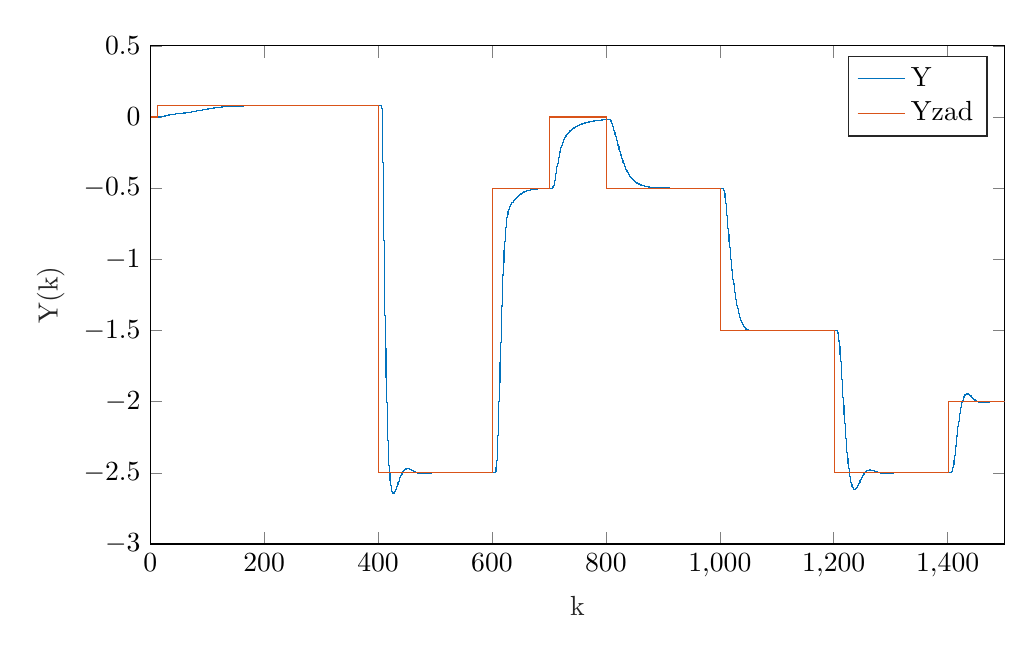
\begin{tikzpicture}

\begin{axis}[%
width=4.272in,
height=2.491in,
at={(0.717in,0.423in)},
scale only axis,
xmin=0,
xmax=1500,
xlabel style={font=\color{white!15!black}},
xlabel={k},
ymin=-3,
ymax=0.5,
ylabel style={font=\color{white!15!black}},
ylabel={Y(k)},
axis background/.style={fill=white},
legend style={legend cell align=left, align=left, draw=white!15!black}
]
\addplot[const plot, color=mycolor1] table[row sep=crcr] {%
1	0\\
2	0\\
3	0\\
4	0\\
5	0\\
6	0\\
7	0\\
8	0\\
9	0\\
10	0\\
11	0\\
12	0\\
13	0\\
14	0\\
15	0\\
16	0\\
17	0.000154169250607201\\
18	0.000599014362772363\\
19	0.00130880300351848\\
20	0.00220217062654026\\
21	0.00319622008800252\\
22	0.00422770609555045\\
23	0.00525645096843976\\
24	0.00626097445080129\\
25	0.00723223810258482\\
26	0.00816824838247504\\
27	0.00907033256810356\\
28	0.00994096202129487\\
29	0.010782681163227\\
30	0.0115976998208832\\
31	0.0123878215723171\\
32	0.0131545069913129\\
33	0.0138989675248674\\
34	0.0146222465338053\\
35	0.0153252761772107\\
36	0.0160089126172521\\
37	0.0166739560904458\\
38	0.0173211615399455\\
39	0.0179512440216993\\
40	0.0185648818805019\\
41	0.0191627190208616\\
42	0.0197453668416531\\
43	0.0203134060426535\\
44	0.0208673883599588\\
45	0.0214078382352751\\
46	0.0219352544115183\\
47	0.0224501114473697\\
48	0.0229528611464689\\
49	0.023443933899863\\
50	0.0239237399426578\\
51	0.0243926705275583\\
52	0.0248510990192198\\
53	0.0252993819141066\\
54	0.0257378597909269\\
55	0.0261668581967655\\
56	0.0265866884738646\\
57	0.0269984094058026\\
58	0.0274066729603351\\
59	0.0278196715877328\\
60	0.028244590072557\\
61	0.0286864198285439\\
62	0.0291481720811577\\
63	0.0296314695820205\\
64	0.0301370789187227\\
65	0.0306652632349687\\
66	0.0312159770531929\\
67	0.0317889583251267\\
68	0.0323837650720554\\
69	0.0329997870204095\\
70	0.0336362484916027\\
71	0.0342922100427685\\
72	0.0349665719627405\\
73	0.0356580808953973\\
74	0.0363653401852987\\
75	0.0370868242394786\\
76	0.0378208969574629\\
77	0.0385658340258443\\
78	0.0393198486204552\\
79	0.0400811198367995\\
80	0.0408478229940821\\
81	0.0416181608346387\\
82	0.0423903945689572\\
83	0.0431628736967594\\
84	0.0439340635672342\\
85	0.044702569725852\\
86	0.0454671582276951\\
87	0.0462267712703802\\
88	0.0469805377022721\\
89	0.0477277781799972\\
90	0.0484680049685582\\
91	0.0492009165836838\\
92	0.0499263876577138\\
93	0.0506444545588942\\
94	0.0513552974047048\\
95	0.0520592191817408\\
96	0.0527566227198109\\
97	0.0534479862707982\\
98	0.0541338384193481\\
99	0.0548147330089979\\
100	0.0554912247100539\\
101	0.0561638457895989\\
102	0.0568330845735358\\
103	0.0574993660183386\\
104	0.0581630347378318\\
105	0.0588243407585823\\
106	0.0594834282065057\\
107	0.0601403270569491\\
108	0.0607949480107177\\
109	0.0614470804894516\\
110	0.0620956865872788\\
111	0.0627352895674209\\
112	0.0633601275892844\\
113	0.0639668258268643\\
114	0.0645538560301352\\
115	0.065120710465891\\
116	0.0656673811674176\\
117	0.066194145566033\\
118	0.06670147889305\\
119	0.0671899870426299\\
120	0.0676603458952306\\
121	0.0681132543643354\\
122	0.0685494041264372\\
123	0.0689694632901712\\
124	0.0693740693682622\\
125	0.0697638275667291\\
126	0.0701393117393171\\
127	0.0705010664762954\\
128	0.0708496095237766\\
129	0.0711854341462491\\
130	0.0715090112683469\\
131	0.0718207913460962\\
132	0.0721212059728008\\
133	0.072410669248104\\
134	0.0726895789458913\\
135	0.0729583175160039\\
136	0.0732172529507471\\
137	0.0734667395422307\\
138	0.0737071185517348\\
139	0.0739387188080774\\
140	0.0741618572484399\\
141	0.074376839412256\\
142	0.07458395989649\\
143	0.0747835027788344\\
144	0.0749757420139474\\
145	0.0751609418067528\\
146	0.0753393569659734\\
147	0.0755112332404001\\
148	0.0756768076398836\\
149	0.0758363087426361\\
150	0.0759899569901124\\
151	0.0761379649705036\\
152	0.0762805376916805\\
153	0.0764178728442837\\
154	0.0765501610555383\\
155	0.076677586134284\\
156	0.0768003253076416\\
157	0.0769185494496848\\
158	0.0770324233024403\\
159	0.0771421056895087\\
160	0.0772477497225726\\
161	0.0773495030010361\\
162	0.0774475078050232\\
163	0.0775419012819522\\
164	0.0776328156268873\\
165	0.0777203782568637\\
166	0.0778047119793726\\
167	0.0778859351551863\\
168	0.0779641618556971\\
169	0.0780395020149398\\
170	0.0781120615764614\\
171	0.0781819426351965\\
172	0.0782492435745061\\
173	0.0783140591985278\\
174	0.0783764808599871\\
175	0.0784365965836116\\
176	0.0784944911852886\\
177	0.0785502463871015\\
178	0.0786039409283772\\
179	0.0786556506728741\\
180	0.0787054487122348\\
181	0.0787534054658268\\
182	0.0787995887770882\\
183	0.0788440640064945\\
184	0.0788868941212578\\
185	0.0789281397818681\\
186	0.0789678594255803\\
187	0.0790061093469513\\
188	0.0790429437755253\\
189	0.0790784149507633\\
190	0.0791125731943122\\
191	0.0791454669797013\\
192	0.0791771429995567\\
193	0.0792076462304157\\
194	0.0792370199952269\\
195	0.079265306023613\\
196	0.0792925445099747\\
197	0.0793187741695103\\
198	0.0793440322922241\\
199	0.0793683547949917\\
200	0.079391776271752\\
201	0.0794143300418904\\
202	0.0794360481968764\\
203	0.0794569616452174\\
204	0.0794771001557881\\
205	0.0794964923995913\\
206	0.0795151659900078\\
207	0.0795331475215866\\
208	0.0795504626074289\\
209	0.0795671359152143\\
210	0.0795831912019187\\
211	0.0795986513472698\\
212	0.0796135383859851\\
213	0.0796278735388369\\
214	0.0796416772425843\\
215	0.0796549691788151\\
216	0.079667768301735\\
217	0.0796800928649421\\
218	0.079691960447224\\
219	0.0797033879774121\\
220	0.0797143917583265\\
221	0.0797249874898456\\
222	0.0797351902911305\\
223	0.0797450147220365\\
224	0.0797544748037391\\
225	0.079763584038604\\
226	0.0797723554293298\\
227	0.079780801497386\\
228	0.0797889343007764\\
229	0.0797967654511491\\
230	0.0798043061302784\\
231	0.079811567105941\\
232	0.0798185587472082\\
233	0.0798252910391765\\
234	0.0798317735971558\\
235	0.0798380156803358\\
236	0.0798440262049487\\
237	0.0798498137569487\\
238	0.0798553866042228\\
239	0.079860752708353\\
240	0.0798659197359443\\
241	0.0798708950695359\\
242	0.0798756858181094\\
243	0.0798802988272097\\
244	0.0798847406886928\\
245	0.0798890177501141\\
246	0.0798931361237692\\
247	0.0798971016954024\\
248	0.0799009201325929\\
249	0.0799045968928313\\
250	0.0799081372312984\\
251	0.0799115462083556\\
252	0.0799148286967602\\
253	0.0799179893886122\\
254	0.079921032802046\\
255	0.0799239632876735\\
256	0.0799267850347899\\
257	0.0799295020773498\\
258	0.0799321182997217\\
259	0.0799346374422309\\
260	0.079937063106496\\
261	0.0799393987605691\\
262	0.0799416477438853\\
263	0.0799438132720291\\
264	0.0799458984413241\\
265	0.079947906233254\\
266	0.0799498395187183\\
267	0.0799517010621317\\
268	0.0799534935253716\\
269	0.0799552194715786\\
270	0.0799568813688174\\
271	0.0799584815936012\\
272	0.0799600224342862\\
273	0.0799615060943401\\
274	0.0799629346954898\\
275	0.0799643102807517\\
276	0.0799656348173511\\
277	0.0799669101995319\\
278	0.0799681382512637\\
279	0.0799693207288473\\
280	0.0799704593234244\\
281	0.0799715556633944\\
282	0.0799726113167409\\
283	0.0799736277932726\\
284	0.0799746065467812\\
285	0.0799755489771186\\
286	0.0799764564321982\\
287	0.0799773302099208\\
288	0.0799781715600302\\
289	0.0799789816858992\\
290	0.07997976174625\\
291	0.0799805128568101\\
292	0.0799812360919077\\
293	0.0799819324860072\\
294	0.079982603035188\\
295	0.0799832486985687\\
296	0.0799838703996782\\
297	0.079984469027776\\
298	0.0799850454391236\\
299	0.0799856004582089\\
300	0.0799861348789247\\
301	0.0799866494657041\\
302	0.0799871449546133\\
303	0.0799876220544044\\
304	0.0799880814475284\\
305	0.0799885237911115\\
306	0.0799889497178941\\
307	0.0799893598371365\\
308	0.0799897547354893\\
309	0.0799901349778328\\
310	0.0799905011080846\\
311	0.0799908536499775\\
312	0.0799911931078084\\
313	0.0799915199671596\\
314	0.0799918346955931\\
315	0.0799921377433194\\
316	0.0799924295438414\\
317	0.0799927105145741\\
318	0.0799929810574419\\
319	0.0799932415594532\\
320	0.0799934923932541\\
321	0.0799937339176612\\
322	0.0799939664781747\\
323	0.079994190407473\\
324	0.0799944060258879\\
325	0.0799946136418632\\
326	0.0799948135523959\\
327	0.0799950060434607\\
328	0.0799951913904189\\
329	0.0799953698584129\\
330	0.0799955417027448\\
331	0.079995707169242\\
332	0.0799958664946084\\
333	0.0799960199067634\\
334	0.0799961676251677\\
335	0.079996309861137\\
336	0.0799964468181447\\
337	0.0799965786921126\\
338	0.0799967056716915\\
339	0.0799968279385304\\
340	0.0799969456675371\\
341	0.0799970590271279\\
342	0.0799971681794686\\
343	0.0799972732807067\\
344	0.0799973744811942\\
345	0.0799974719257035\\
346	0.0799975657536336\\
347	0.0799976560992101\\
348	0.0799977430916771\\
349	0.079997826855482\\
350	0.0799979075104533\\
351	0.0799979851719725\\
352	0.0799980599511388\\
353	0.0799981319549279\\
354	0.0799982012863456\\
355	0.0799982680445746\\
356	0.0799983323251165\\
357	0.0799983942199285\\
358	0.0799984538175549\\
359	0.079998511203254\\
360	0.0799985664591197\\
361	0.0799986196641988\\
362	0.079998670894605\\
363	0.0799987202236264\\
364	0.0799987677218316\\
365	0.07999881345717\\
366	0.079998857495069\\
367	0.0799988998985279\\
368	0.0799989407282077\\
369	0.0799989800425181\\
370	0.0799990178977009\\
371	0.0799990543479107\\
372	0.079999089445292\\
373	0.0799991232400542\\
374	0.0799991557805431\\
375	0.0799991871133102\\
376	0.0799992172831794\\
377	0.0799992463333108\\
378	0.0799992743052627\\
379	0.0799993012390511\\
380	0.0799993271732068\\
381	0.0799993521448305\\
382	0.079999376189646\\
383	0.0799993993420513\\
384	0.0799994216351675\\
385	0.0799994431008867\\
386	0.0799994637699172\\
387	0.0799994836718277\\
388	0.0799995028350893\\
389	0.0799995212871165\\
390	0.0799995390543065\\
391	0.0799995561620766\\
392	0.0799995726349007\\
393	0.0799995884963445\\
394	0.079999603769099\\
395	0.0799996184750131\\
396	0.0799996326351249\\
397	0.0799996462696913\\
398	0.0799996593982178\\
399	0.0799996720394857\\
400	0.0799996842115794\\
401	0.079999695931912\\
402	0.0799997072172505\\
403	0.0799997180837393\\
404	0.0799997285469238\\
405	0.0799997386217725\\
406	0.0595473087305461\\
407	-0.0895453023859561\\
408	-0.317601364446208\\
409	-0.585602879654245\\
410	-0.866000976556553\\
411	-1.14015351952599\\
412	-1.39619437723045\\
413	-1.62729388768736\\
414	-1.83026405234094\\
415	-2.0044604441061\\
416	-2.15093425984756\\
417	-2.27179127575127\\
418	-2.36971885223333\\
419	-2.44764699168049\\
420	-2.50851436665324\\
421	-2.55497555452166\\
422	-2.58934959622986\\
423	-2.61367461972667\\
424	-2.6297431136223\\
425	-2.63911803286258\\
426	-2.64312278713509\\
427	-2.64286032513737\\
428	-2.63924390266816\\
429	-2.63302705289787\\
430	-2.62483172395098\\
431	-2.61517347393721\\
432	-2.60448368371813\\
433	-2.59312776087598\\
434	-2.58141876118503\\
435	-2.56962673499348\\
436	-2.55798460294183\\
437	-2.54669155609279\\
438	-2.53591494988006\\
439	-2.52579150184615\\
440	-2.51642838263964\\
441	-2.50790456363892\\
442	-2.50027258854142\\
443	-2.49356078807699\\
444	-2.48777586058448\\
445	-2.48290569128038\\
446	-2.47892230210856\\
447	-2.47578474924092\\
448	-2.47344185438049\\
449	-2.47183471117239\\
450	-2.47089893583227\\
451	-2.47056665283065\\
452	-2.47076822026179\\
453	-2.47143370990855\\
454	-2.47249416245801\\
455	-2.47388263936777\\
456	-2.47553509144593\\
457	-2.47739106175195\\
458	-2.4793942379234\\
459	-2.48149286702806\\
460	-2.48364004472812\\
461	-2.4857938898886\\
462	-2.48791761559929\\
463	-2.48997950769605\\
464	-2.49195282206546\\
465	-2.49381561213996\\
466	-2.49555049788807\\
467	-2.49714438743916\\
468	-2.49858816201268\\
469	-2.49987633411982\\
470	-2.50100668817242\\
471	-2.50197991172214\\
472	-2.50279922461324\\
473	-2.50347001239478\\
474	-2.5039994694306\\
475	-2.50439625628342\\
476	-2.50467017514355\\
477	-2.50483186632328\\
478	-2.50489252814578\\
479	-2.50486366191861\\
480	-2.50475684309558\\
481	-2.50458351919431\\
482	-2.50435483455081\\
483	-2.50408148155657\\
484	-2.50377357763933\\
485	-2.50344056691632\\
486	-2.50309114516917\\
487	-2.50273320656263\\
488	-2.5023738103529\\
489	-2.50201916570534\\
490	-2.5016746326613\\
491	-2.50134473725721\\
492	-2.50103319880123\\
493	-2.50074296734942\\
494	-2.50047626948962\\
495	-2.50023466063235\\
496	-2.50001908211941\\
497	-2.49982992158741\\
498	-2.4996670751624\\
499	-2.49953001020671\\
500	-2.49941782748962\\
501	-2.49932932180325\\
502	-2.49926304019399\\
503	-2.49921733712365\\
504	-2.4991904260124\\
505	-2.49918042674524\\
506	-2.49918540884466\\
507	-2.49920343012226\\
508	-2.49923257072231\\
509	-2.49927096255862\\
510	-2.4993168142236\\
511	-2.49936843151503\\
512	-2.49942423378122\\
513	-2.49948276633088\\
514	-2.49954270918902\\
515	-2.49960288250664\\
516	-2.49966224894956\\
517	-2.49971991340191\\
518	-2.49977512032299\\
519	-2.49982724909321\\
520	-2.49987580767692\\
521	-2.49992042491706\\
522	-2.49996084176067\\
523	-2.49999690169472\\
524	-2.50002854065037\\
525	-2.50005577661067\\
526	-2.50007869913243\\
527	-2.50009745896843\\
528	-2.50011225795111\\
529	-2.50012333927496\\
530	-2.50013097829075\\
531	-2.50013547390238\\
532	-2.5001371406358\\
533	-2.50013630142953\\
534	-2.50013328117803\\
535	-2.50012840104301\\
536	-2.50012197353251\\
537	-2.50011429833536\\
538	-2.50010565888695\\
539	-2.50009631963337\\
540	-2.50008652395311\\
541	-2.50007649268974\\
542	-2.50006642324429\\
543	-2.50005648917324\\
544	-2.50004684023621\\
545	-2.50003760283658\\
546	-2.50002888079926\\
547	-2.50002075643038\\
548	-2.50001329180649\\
549	-2.50000653024295\\
550	-2.50000049789485\\
551	-2.49999520544701\\
552	-2.4999906498538\\
553	-2.49998681609332\\
554	-2.49998367890486\\
555	-2.49998120448243\\
556	-2.4999793521016\\
557	-2.49997807566042\\
558	-2.49997732511944\\
559	-2.49997704782909\\
560	-2.49997718973618\\
561	-2.49997769646424\\
562	-2.49997851426528\\
563	-2.49997959084299\\
564	-2.4999808760494\\
565	-2.4999823224592\\
566	-2.49998388582711\\
567	-2.49998552543519\\
568	-2.49998720433801\\
569	-2.49998888951403\\
570	-2.49999055193258\\
571	-2.49999216654547\\
572	-2.49999371221297\\
573	-2.49999517157341\\
574	-2.49999653086562\\
575	-2.49999777971304\\
576	-2.49999891087785\\
577	-2.49999991999298\\
578	-2.50000080527926\\
579	-2.50000156725424\\
580	-2.50000220843859\\
581	-2.50000273306546\\
582	-2.500003146797\\
583	-2.50000345645225\\
584	-2.5000036697493\\
585	-2.50000379506435\\
586	-2.50000384120968\\
587	-2.50000381723182\\
588	-2.5000037322308\\
589	-2.50000359520097\\
590	-2.50000341489331\\
591	-2.50000319969891\\
592	-2.50000295755291\\
593	-2.50000269585804\\
594	-2.50000242142655\\
595	-2.50000214043924\\
596	-2.50000185842015\\
597	-2.50000158022542\\
598	-2.50000131004472\\
599	-2.50000105141368\\
600	-2.50000080723575\\
601	-2.50000057981189\\
602	-2.50000037087681\\
603	-2.50000018164003\\
604	-2.50000001283082\\
605	-2.49999986474551\\
606	-2.49029713196076\\
607	-2.46205975761276\\
608	-2.41105932586453\\
609	-2.33659780386956\\
610	-2.24055834023666\\
611	-2.12655374474973\\
612	-1.99919097643437\\
613	-1.86346880317636\\
614	-1.72431040198092\\
615	-1.58622210726324\\
616	-1.45306416570259\\
617	-1.32791788736969\\
618	-1.21303398259985\\
619	-1.1098474687952\\
620	-1.01904456365462\\
621	-0.940666619555204\\
622	-0.874236078589913\\
623	-0.818890292363295\\
624	-0.773508067497102\\
625	-0.736792774194494\\
626	-0.707409088704036\\
627	-0.684076659100913\\
628	-0.665622029976745\\
629	-0.651006981325861\\
630	-0.639340355233981\\
631	-0.629878631380483\\
632	-0.622018933864507\\
633	-0.615287080840366\\
634	-0.609322614955919\\
635	-0.603862313310234\\
636	-0.598723360610791\\
637	-0.593787111314503\\
638	-0.588984132023485\\
639	-0.58428099374819\\
640	-0.579669077860306\\
641	-0.575155478192324\\
642	-0.570755933292851\\
643	-0.566489612592069\\
644	-0.562375509126934\\
645	-0.558430156479098\\
646	-0.554666361880849\\
647	-0.551092721310107\\
648	-0.547713683477821\\
649	-0.544529955925059\\
650	-0.541539092009864\\
651	-0.538736141345827\\
652	-0.536114284952814\\
653	-0.533665407948689\\
654	-0.531380586469178\\
655	-0.529250482175358\\
656	-0.527265648322456\\
657	-0.525416757275716\\
658	-0.523694761899087\\
659	-0.522091003566526\\
660	-0.520597278570202\\
661	-0.519205873092799\\
662	-0.517909575118117\\
663	-0.516701669941649\\
664	-0.515575924444732\\
665	-0.514526564057769\\
666	-0.51354824538504\\
667	-0.512636026635029\\
668	-0.511785337408083\\
669	-0.510991948962044\\
670	-0.510251945740153\\
671	-0.50956169867849\\
672	-0.508917840596082\\
673	-0.508317243800391\\
674	-0.50775699990908\\
675	-0.507234401792129\\
676	-0.506746927473222\\
677	-0.506292225791531\\
678	-0.50586810360996\\
679	-0.505472514358255\\
680	-0.505103547714061\\
681	-0.504759420247159\\
682	-0.504438466877848\\
683	-0.504139133026515\\
684	-0.503859967355812\\
685	-0.503599615028034\\
686	-0.503356811417832\\
687	-0.503130376234214\\
688	-0.502919208016185\\
689	-0.502722278973839\\
690	-0.502538630151787\\
691	-0.502367366895182\\
692	-0.502207654600775\\
693	-0.502058714736818\\
694	-0.501919821116611\\
695	-0.501790296411191\\
696	-0.501669508887287\\
697	-0.501556869357258\\
698	-0.501451828328325\\
699	-0.501353873338985\\
700	-0.501262526471114\\
701	-0.501177342026851\\
702	-0.501097904359909\\
703	-0.501023825851552\\
704	-0.500954745021957\\
705	-0.500890324768246\\
706	-0.498379068912454\\
707	-0.491527671686034\\
708	-0.479811611392552\\
709	-0.46359654756943\\
710	-0.44374848387263\\
711	-0.421338640726875\\
712	-0.397441143995627\\
713	-0.373011430199162\\
714	-0.348826937238824\\
715	-0.325470999756983\\
716	-0.303343597125825\\
717	-0.28268652183036\\
718	-0.263614344979497\\
719	-0.246145681624818\\
720	-0.230231580849416\\
721	-0.215779478542266\\
722	-0.202672213390225\\
723	-0.190782268814573\\
724	-0.179981782475501\\
725	-0.170149045900998\\
726	-0.161172994114142\\
727	-0.152954443308265\\
728	-0.145405817645854\\
729	-0.138450445961044\\
730	-0.132021628739238\\
731	-0.126061600641711\\
732	-0.120520468245713\\
733	-0.115355176344638\\
734	-0.110528539184809\\
735	-0.10600836005166\\
736	-0.101766652038562\\
737	-0.0977789641912291\\
738	-0.0940238104817912\\
739	-0.0904821942228506\\
740	-0.0871372174729263\\
741	-0.0839737634848322\\
742	-0.0809782400036702\\
743	-0.0781383718951874\\
744	-0.0754430328515005\\
745	-0.0728821074922524\\
746	-0.0704463766252779\\
747	-0.0681274205978042\\
748	-0.0659175366089159\\
749	-0.0638096667472674\\
750	-0.0617973345303135\\
751	-0.0598745884475474\\
752	-0.0580359514930063\\
753	-0.0562763759681332\\
754	-0.0545912030021052\\
755	-0.0529761263228377\\
756	-0.0514272880361664\\
757	-0.0499416493666086\\
758	-0.048516695519961\\
759	-0.0471499946044195\\
760	-0.0458390328386544\\
761	-0.0445812003805234\\
762	-0.0433738412072066\\
763	-0.0422143166134579\\
764	-0.0411000594197606\\
765	-0.0400286119757196\\
766	-0.0389976485001642\\
767	-0.038004985025829\\
768	-0.0370485806297726\\
769	-0.0361265331039307\\
770	-0.035237071444852\\
771	-0.0343785468157871\\
772	-0.0335494230551212\\
773	-0.0327482673808375\\
774	-0.0319737416474141\\
775	-0.031224594318897\\
776	-0.0304996532023189\\
777	-0.0297978189169318\\
778	-0.0291180590399407\\
779	-0.0284594028560666\\
780	-0.0278209366374569\\
781	-0.02720179938618\\
782	-0.0266011789799545\\
783	-0.0260183086706017\\
784	-0.0254524638928304\\
785	-0.0249029593478664\\
786	-0.024369146332075\\
787	-0.0238504102852115\\
788	-0.0233461685364904\\
789	-0.0228558682294933\\
790	-0.0223789844092248\\
791	-0.021915018256513\\
792	-0.0214634954565432\\
793	-0.0210239646896797\\
794	-0.0205959962339234\\
795	-0.0201791806694008\\
796	-0.019773127676217\\
797	-0.0193774649178362\\
798	-0.0189918370028963\\
799	-0.0186159045190352\\
800	-0.0182493431329018\\
801	-0.0178918427510619\\
802	-0.0175431067369929\\
803	-0.017202851179793\\
804	-0.0168708042106194\\
805	-0.0165467053632232\\
806	-0.0174712730161749\\
807	-0.0207660389654935\\
808	-0.0265389450725452\\
809	-0.0345028918455527\\
810	-0.0442580358825786\\
811	-0.0554117953686117\\
812	-0.0676328304054761\\
813	-0.0806610927063029\\
814	-0.0942967647251742\\
815	-0.10838454049254\\
816	-0.122799997952004\\
817	-0.137439704697475\\
818	-0.152214571637721\\
819	-0.167045480545041\\
820	-0.181860390925529\\
821	-0.196592446698577\\
822	-0.211178838338209\\
823	-0.225560289666341\\
824	-0.239681062077052\\
825	-0.253489350243644\\
826	-0.266936272211136\\
827	-0.279977245699301\\
828	-0.292573898308837\\
829	-0.304695247960674\\
830	-0.316318207235865\\
831	-0.327427509905236\\
832	-0.338015192364655\\
833	-0.348079776503318\\
834	-0.357625293440711\\
835	-0.366660266182268\\
836	-0.375196739669178\\
837	-0.383249415153668\\
838	-0.390834917123914\\
839	-0.3979711981015\\
840	-0.404677070779164\\
841	-0.410971847987974\\
842	-0.416875067763071\\
843	-0.422406281731046\\
844	-0.427584888518803\\
845	-0.432429998443053\\
846	-0.436960324596798\\
847	-0.441194087881641\\
848	-0.445148932657512\\
849	-0.448841854556113\\
850	-0.452289142235824\\
851	-0.455506334357174\\
852	-0.458508192156739\\
853	-0.461308687001716\\
854	-0.463921001449152\\
855	-0.466357541736792\\
856	-0.468629959333175\\
857	-0.470749179147425\\
858	-0.47272543218283\\
859	-0.474568290737932\\
860	-0.476286704642658\\
861	-0.477889037405978\\
862	-0.479383101504105\\
863	-0.480776192330345\\
864	-0.482075120550638\\
865	-0.483286242764895\\
866	-0.484415490465255\\
867	-0.485468397351318\\
868	-0.486450125086007\\
869	-0.487365487574055\\
870	-0.488218973835398\\
871	-0.489014769534818\\
872	-0.489756777220594\\
873	-0.490448635320268\\
874	-0.491093735940684\\
875	-0.491695241521263\\
876	-0.49225610039264\\
877	-0.49277906129621\\
878	-0.493266686922799\\
879	-0.493721366530112\\
880	-0.494145327698625\\
881	-0.494540647284225\\
882	-0.494909261623491\\
883	-0.495252976044286\\
884	-0.495573473730738\\
885	-0.495872323987939\\
886	-0.496150989948095\\
887	-0.496410835756452\\
888	-0.496653133272282\\
889	-0.496879068317508\\
890	-0.497089746503156\\
891	-0.497286198661775\\
892	-0.497469385912083\\
893	-0.497640204380412\\
894	-0.497799489601991\\
895	-0.497948020623637\\
896	-0.498086523828051\\
897	-0.498215676498622\\
898	-0.498336110142381\\
899	-0.498448413587576\\
900	-0.498553135871227\\
901	-0.498650788930956\\
902	-0.498741850114417\\
903	-0.498826764518721\\
904	-0.498905947171417\\
905	-0.498979785063765\\
906	-0.499048639046344\\
907	-0.499112845596304\\
908	-0.499172718464985\\
909	-0.499228550214008\\
910	-0.499280613647391\\
911	-0.499329163146757\\
912	-0.499374435916183\\
913	-0.499416653142837\\
914	-0.499456021079103\\
915	-0.499492732051517\\
916	-0.499526965401474\\
917	-0.499558888362332\\
918	-0.499588656877222\\
919	-0.499616416361571\\
920	-0.499642302414093\\
921	-0.49966644147973\\
922	-0.499688951467789\\
923	-0.499709942328317\\
924	-0.499729516589533\\
925	-0.499747769858951\\
926	-0.499764791290647\\
927	-0.499780664020967\\
928	-0.499795465574803\\
929	-0.499809268244425\\
930	-0.499822139442732\\
931	-0.499834142032648\\
932	-0.499845334634266\\
933	-0.499855771911258\\
934	-0.499865504837944\\
935	-0.499874580948329\\
936	-0.499883044568317\\
937	-0.499890937032264\\
938	-0.499898296884891\\
939	-0.499905160069579\\
940	-0.499911560103948\\
941	-0.499917528243581\\
942	-0.499923093634698\\
943	-0.499928283456524\\
944	-0.499933123054045\\
945	-0.499937636061803\\
946	-0.499941844519338\\
947	-0.49994576897883\\
948	-0.499949428605486\\
949	-0.499952841271143\\
950	-0.499956023641554\\
951	-0.499958991257787\\
952	-0.499961758612129\\
953	-0.499964339218859\\
954	-0.499966745680258\\
955	-0.499968989748153\\
956	-0.499971082381311\\
957	-0.499973033798961\\
958	-0.499974853530698\\
959	-0.499976550463031\\
960	-0.499978132882774\\
961	-0.499979608517521\\
962	-0.499980984573383\\
963	-0.49998226777018\\
964	-0.499983464374259\\
965	-0.499984580229096\\
966	-0.499985620783832\\
967	-0.499986591119885\\
968	-0.499987495975766\\
969	-0.499988339770219\\
970	-0.499989126623798\\
971	-0.499989860378994\\
972	-0.499990544618996\\
973	-0.499991182685191\\
974	-0.499991777693481\\
975	-0.499992332549501\\
976	-0.499992849962805\\
977	-0.499993332460103\\
978	-0.499993782397594\\
979	-0.499994201972478\\
980	-0.499994593233683\\
981	-0.499994958091868\\
982	-0.499995298328761\\
983	-0.499995615605854\\
984	-0.499995911472515\\
985	-0.499996187373562\\
986	-0.499996444656311\\
987	-0.49999668457716\\
988	-0.499996908307721\\
989	-0.499997116940545\\
990	-0.499997311494455\\
991	-0.499997492919522\\
992	-0.499997662101703\\
993	-0.499997819867172\\
994	-0.499997966986348\\
995	-0.499998104177662\\
996	-0.499998232111064\\
997	-0.499998351411296\\
998	-0.499998462660938\\
999	-0.499998566403258\\
1000	-0.499998663144865\\
1001	-0.499998753358178\\
1002	-0.499998837483739\\
1003	-0.49999891593236\\
1004	-0.499998989087131\\
1005	-0.49999905730529\\
1006	-0.504737300639583\\
1007	-0.517567647075985\\
1008	-0.539192624938858\\
1009	-0.568777220647052\\
1010	-0.604826688774357\\
1011	-0.645676151577607\\
1012	-0.689726234601704\\
1013	-0.735566954777115\\
1014	-0.782034524661009\\
1015	-0.828223561603972\\
1016	-0.873470820967731\\
1017	-0.917322555774211\\
1018	-0.959494555775519\\
1019	-0.999831325973937\\
1020	-1.03826864985561\\
1021	-1.07480195491153\\
1022	-1.10946147315616\\
1023	-1.14229416171387\\
1024	-1.17335168362428\\
1025	-1.20268338922861\\
1026	-1.23032558352012\\
1027	-1.25630371602347\\
1028	-1.28063873431065\\
1029	-1.30335219877459\\
1030	-1.32446994727251\\
1031	-1.34402433707059\\
1032	-1.36205525783303\\
1033	-1.37861019289431\\
1034	-1.39374361967419\\
1035	-1.40751601186802\\
1036	-1.41999265538776\\
1037	-1.43124243157009\\
1038	-1.44133666579513\\
1039	-1.45034809382728\\
1040	-1.45834996445612\\
1041	-1.46541527520581\\
1042	-1.47161612619739\\
1043	-1.47702317316371\\
1044	-1.48170516152079\\
1045	-1.48572852700258\\
1046	-1.48915706594213\\
1047	-1.49205164889053\\
1048	-1.49446997195343\\
1049	-1.49646635120937\\
1050	-1.49809156524833\\
1051	-1.49939274930187\\
1052	-1.50041334219224\\
1053	-1.50119308493974\\
1054	-1.50176806773256\\
1055	-1.50217082030129\\
1056	-1.50243043963324\\
1057	-1.5025727483953\\
1058	-1.50262047733179\\
1059	-1.50259346515929\\
1060	-1.50250886998288\\
1061	-1.50238138690842\\
1062	-1.5022234672413\\
1063	-1.5020455353857\\
1064	-1.50185620024984\\
1065	-1.50166245859996\\
1066	-1.50146988835636\\
1067	-1.50128283037019\\
1068	-1.50110455766442\\
1069	-1.50093743149247\\
1070	-1.50078304388802\\
1071	-1.50064234665554\\
1072	-1.50051576698781\\
1073	-1.50040331009506\\
1074	-1.50030464939408\\
1075	-1.50021920493418\\
1076	-1.50014621083396\\
1077	-1.50008477256914\\
1078	-1.50003391499085\\
1079	-1.49999262196865\\
1080	-1.49995986854684\\
1081	-1.49993464647926\\
1082	-1.49991598397184\\
1083	-1.49990296041459\\
1084	-1.49989471683147\\
1085	-1.49989046271718\\
1086	-1.49988947986964\\
1087	-1.49989112376499\\
1088	-1.49989482296157\\
1089	-1.49990007696075\\
1090	-1.49990645289717\\
1091	-1.4999135813787\\
1092	-1.49992115174844\\
1093	-1.49992890699689\\
1094	-1.49993663851274\\
1095	-1.49994418082481\\
1096	-1.49995140645614\\
1097	-1.49995822098333\\
1098	-1.49996455837044\\
1099	-1.49997037662579\\
1100	-1.499975653813\\
1101	-1.49998038443283\\
1102	-1.49998457618067\\
1103	-1.49998824707516\\
1104	-1.49999142294565\\
1105	-1.49999413526125\\
1106	-1.49999641927937\\
1107	-1.49999831248976\\
1108	-1.49999985332785\\
1109	-1.50000108013082\\
1110	-1.50000203030988\\
1111	-1.50000273971263\\
1112	-1.5000032421509\\
1113	-1.50000356907039\\
1114	-1.50000374934054\\
1115	-1.5000038091445\\
1116	-1.50000377195113\\
1117	-1.50000365855293\\
1118	-1.50000348715537\\
1119	-1.50000327350523\\
1120	-1.50000303104699\\
1121	-1.50000277109817\\
1122	-1.5000025030357\\
1123	-1.50000223448705\\
1124	-1.50000197152086\\
1125	-1.50000171883291\\
1126	-1.50000147992433\\
1127	-1.50000125726964\\
1128	-1.50000105247304\\
1129	-1.50000086641186\\
1130	-1.50000069936659\\
1131	-1.50000055113749\\
1132	-1.50000042114782\\
1133	-1.50000030853419\\
1134	-1.50000021222476\\
1135	-1.50000013100591\\
1136	-1.50000006357838\\
1137	-1.50000000860374\\
1138	-1.49999996474221\\
1139	-1.49999993068267\\
1140	-1.49999990516592\\
1141	-1.49999988700196\\
1142	-1.49999987508219\\
1143	-1.49999986838733\\
1144	-1.49999986599162\\
1145	-1.49999986706422\\
1146	-1.49999987086812\\
1147	-1.4999998767572\\
1148	-1.49999988417189\\
1149	-1.49999989263384\\
1150	-1.49999990173976\\
1151	-1.49999991115505\\
1152	-1.499999920607\\
1153	-1.49999992987819\\
1154	-1.49999993879991\\
1155	-1.49999994724592\\
1156	-1.49999995512649\\
1157	-1.4999999623829\\
1158	-1.49999996898237\\
1159	-1.49999997491344\\
1160	-1.49999998018188\\
1161	-1.49999998480694\\
1162	-1.49999998881824\\
1163	-1.49999999225292\\
1164	-1.49999999515328\\
1165	-1.4999999975648\\
1166	-1.49999999953446\\
1167	-1.50000000110939\\
1168	-1.50000000233579\\
1169	-1.50000000325811\\
1170	-1.50000000391839\\
1171	-1.50000000435586\\
1172	-1.50000000460663\\
1173	-1.50000000470352\\
1174	-1.50000000467603\\
1175	-1.50000000455035\\
1176	-1.50000000434947\\
1177	-1.5000000040933\\
1178	-1.50000000379891\\
1179	-1.5000000034807\\
1180	-1.50000000315063\\
1181	-1.50000000281847\\
1182	-1.50000000249203\\
1183	-1.50000000217738\\
1184	-1.50000000187908\\
1185	-1.5000000016004\\
1186	-1.50000000134349\\
1187	-1.50000000110958\\
1188	-1.50000000089913\\
1189	-1.50000000071199\\
1190	-1.50000000054753\\
1191	-1.50000000040473\\
1192	-1.50000000028231\\
1193	-1.50000000017879\\
1194	-1.50000000009259\\
1195	-1.50000000002207\\
1196	-1.49999999996555\\
1197	-1.49999999992143\\
1198	-1.49999999988812\\
1199	-1.49999999986415\\
1200	-1.49999999984812\\
1201	-1.49999999983877\\
1202	-1.49999999983491\\
1203	-1.49999999983552\\
1204	-1.49999999983965\\
1205	-1.4999999998465\\
1206	-1.50464349001927\\
1207	-1.51772168398619\\
1208	-1.54072386360656\\
1209	-1.57362727174537\\
1210	-1.61548210059437\\
1211	-1.66483742620488\\
1212	-1.72003983997287\\
1213	-1.77943065798515\\
1214	-1.841465605719\\
1215	-1.90477782252562\\
1216	-1.96820159456451\\
1217	-2.03077076785152\\
1218	-2.09170252687016\\
1219	-2.15037429341018\\
1220	-2.20629899965717\\
1221	-2.25910196620652\\
1222	-2.30850107173519\\
1223	-2.35429080109194\\
1224	-2.3963300410081\\
1225	-2.43453308241949\\
1226	-2.46885552001427\\
1227	-2.49929180900994\\
1228	-2.52587669097225\\
1229	-2.54868526798294\\
1230	-2.56783161657823\\
1231	-2.58346603154498\\
1232	-2.59577114117406\\
1233	-2.60495721285229\\
1234	-2.61125697507237\\
1235	-2.61492024709018\\
1236	-2.61620861249635\\
1237	-2.61539031344445\\
1238	-2.61273548786542\\
1239	-2.60851182752376\\
1240	-2.60298070150014\\
1241	-2.59639376661049\\
1242	-2.58899007121925\\
1243	-2.58099364937339\\
1244	-2.57261159590017\\
1245	-2.56403260832891\\
1246	-2.55542599024604\\
1247	-2.54694107263761\\
1248	-2.53870702166296\\
1249	-2.53083300546969\\
1250	-2.52340868705125\\
1251	-2.51650500496845\\
1252	-2.51017519958571\\
1253	-2.50445603977344\\
1254	-2.49936920404241\\
1255	-2.49492277079898\\
1256	-2.49111277465453\\
1257	-2.48792478919276\\
1258	-2.4853355009479\\
1259	-2.48331424423152\\
1260	-2.48182447155229\\
1261	-2.48082513944101\\
1262	-2.48027199432493\\
1263	-2.48011874754705\\
1264	-2.48031813261383\\
1265	-2.48082284123292\\
1266	-2.48158633764321\\
1267	-2.48256355323846\\
1268	-2.48371146548417\\
1269	-2.48498956668402\\
1270	-2.48636022933501\\
1271	-2.48778897566815\\
1272	-2.48924465955054\\
1273	-2.4906995692662\\
1274	-2.49212945983604\\
1275	-2.4935135235137\\
1276	-2.49483430693458\\
1277	-2.49607758312422\\
1278	-2.49723218621235\\
1279	-2.49828981626959\\
1280	-2.49924482120111\\
1281	-2.5000939621098\\
1282	-2.50083616799364\\
1283	-2.50147228507746\\
1284	-2.50200482550816\\
1285	-2.50243771957236\\
1286	-2.50277607503311\\
1287	-2.50302594663426\\
1288	-2.50319411829196\\
1289	-2.50328789998831\\
1290	-2.50331494090519\\
1291	-2.50328305989151\\
1292	-2.50320009394607\\
1293	-2.50307376502442\\
1294	-2.5029115651419\\
1295	-2.50272065944862\\
1296	-2.50250780669458\\
1297	-2.50227929628586\\
1298	-2.502040900953\\
1299	-2.50179784391101\\
1300	-2.50155477928364\\
1301	-2.50131578449115\\
1302	-2.50108436325816\\
1303	-2.50086345788295\\
1304	-2.50065546942005\\
1305	-2.50046228445912\\
1306	-2.50028530723388\\
1307	-2.50012549586046\\
1308	-2.49998340158298\\
1309	-2.49985920999194\\
1310	-2.49975278327599\\
1311	-2.49966370266636\\
1312	-2.49959131033488\\
1313	-2.49953475010737\\
1314	-2.49949300645396\\
1315	-2.49946494131386\\
1316	-2.49944932840421\\
1317	-2.49944488474859\\
1318	-2.49945029924072\\
1319	-2.49946425813207\\
1320	-2.49948546739757\\
1321	-2.4995126719922\\
1322	-2.49954467206164\\
1323	-2.49958033621374\\
1324	-2.49961861199359\\
1325	-2.49965853373399\\
1326	-2.49969922797608\\
1327	-2.49973991667098\\
1328	-2.4997799183846\\
1329	-2.49981864773342\\
1330	-2.49985561328042\\
1331	-2.49989041411752\\
1332	-2.49992273535497\\
1333	-2.49995234272882\\
1334	-2.49997907652619\\
1335	-2.50000284501497\\
1336	-2.50002361754915\\
1337	-2.50004141750575\\
1338	-2.5000563151925\\
1339	-2.50006842084854\\
1340	-2.5000778778441\\
1341	-2.50008485616816\\
1342	-2.50008954627771\\
1343	-2.50009215336662\\
1344	-2.50009289209831\\
1345	-2.5000919818328\\
1346	-2.50008964236704\\
1347	-2.50008609019599\\
1348	-2.50008153529291\\
1349	-2.50007617839806\\
1350	-2.50007020879855\\
1351	-2.50006380257548\\
1352	-2.50005712128984\\
1353	-2.50005031107482\\
1354	-2.5000435020994\\
1355	-2.50003680836603\\
1356	-2.50003032780451\\
1357	-2.50002414262367\\
1358	-2.50001831988305\\
1359	-2.50001291224765\\
1360	-2.50000795889039\\
1361	-2.5000034865089\\
1362	-2.49999951042532\\
1363	-2.4999960357404\\
1364	-2.4999930585159\\
1365	-2.49999056696177\\
1366	-2.4999885426078\\
1367	-2.49998696144191\\
1368	-2.49998579500013\\
1369	-2.49998501139608\\
1370	-2.49998457628008\\
1371	-2.4999844537206\\
1372	-2.4999846070029\\
1373	-2.49998499934172\\
1374	-2.49998559450679\\
1375	-2.49998635736136\\
1376	-2.49998725431567\\
1377	-2.49998825369822\\
1378	-2.49998932604879\\
1379	-2.49999044433809\\
1380	-2.49999158411934\\
1381	-2.49999272361785\\
1382	-2.49999384376459\\
1383	-2.49999492818028\\
1384	-2.49999596311638\\
1385	-2.49999693735926\\
1386	-2.49999784210375\\
1387	-2.49999867080204\\
1388	-2.49999941899345\\
1389	-2.50000008412032\\
1390	-2.50000066533485\\
1391	-2.50000116330122\\
1392	-2.50000157999689\\
1393	-2.50000191851659\\
1394	-2.50000218288182\\
1395	-2.50000237785847\\
1396	-2.50000250878462\\
1397	-2.50000258141002\\
1398	-2.50000260174867\\
1399	-2.50000257594521\\
1400	-2.50000251015569\\
1401	-2.50000241044293\\
1402	-2.50000228268648\\
1403	-2.50000213250676\\
1404	-2.50000196520295\\
1405	-2.50000178570402\\
1406	-2.49763202210429\\
1407	-2.49080186011684\\
1408	-2.47855528524739\\
1409	-2.46075147511689\\
1410	-2.43780340570629\\
1411	-2.41046577401483\\
1412	-2.37967006952062\\
1413	-2.34640377017526\\
1414	-2.31162769543356\\
1415	-2.27622419719124\\
1416	-2.24096874889716\\
1417	-2.20651819185056\\
1418	-2.17341003657551\\
1419	-2.14206849558932\\
1420	-2.11281413711001\\
1421	-2.08587508105746\\
1422	-2.06139846248385\\
1423	-2.03946146460969\\
1424	-2.02008160342829\\
1425	-2.00322617055714\\
1426	-1.98882483404376\\
1427	-1.97677604621001\\
1428	-1.96695152425849\\
1429	-1.95920115220778\\
1430	-1.95335813836305\\
1431	-1.94924421857844\\
1432	-1.9466746805741\\
1433	-1.94546300610556\\
1434	-1.94542497672286\\
1435	-1.94638214760001\\
1436	-1.94816465051193\\
1437	-1.95061333450373\\
1438	-1.95358128806323\\
1439	-1.95693480937684\\
1440	-1.96055390294772\\
1441	-1.96433238377086\\
1442	-1.96817766691382\\
1443	-1.97201031308756\\
1444	-1.97576339155304\\
1445	-1.97938171195196\\
1446	-1.98282096083072\\
1447	-1.98604678703338\\
1448	-1.989033864736\\
1449	-1.99176495271122\\
1450	-1.9942299644474\\
1451	-1.99642506090095\\
1452	-1.99835177559626\\
1453	-2.00001618018795\\
1454	-2.00142809722506\\
1455	-2.00260036556755\\
1456	-2.00354816263982\\
1457	-2.00428838645293\\
1458	-2.00483909910491\\
1459	-2.00521903230826\\
1460	-2.0054471544261\\
1461	-2.00554229755032\\
1462	-2.00552284234124\\
1463	-2.00540645767858\\
1464	-2.0052098916446\\
1465	-2.00494880996758\\
1466	-2.00463767779676\\
1467	-2.00428968050359\\
1468	-2.00391667914453\\
1469	-2.00352919625245\\
1470	-2.00313642772626\\
1471	-2.00274627674694\\
1472	-2.0023654058538\\
1473	-2.0019993035565\\
1474	-2.00165236212837\\
1475	-2.00132796351644\\
1476	-2.00102857060693\\
1477	-2.00075582139373\\
1478	-2.00051062390728\\
1479	-2.00029325006451\\
1480	-2.00010342689468\\
1481	-1.99994042387481\\
1482	-1.99980313536997\\
1483	-1.99969015741508\\
1484	-1.99959985829443\\
1485	-1.99953044257123\\
1486	-1.99948000839302\\
1487	-1.99944659804872\\
1488	-1.99942824188047\\
1489	-1.99942299575976\\
1490	-1.99942897242319\\
1491	-1.9994443670303\\
1492	-1.99946747735635\\
1493	-1.99949671906767\\
1494	-1.99953063654871\\
1495	-1.99956790975923\\
1496	-1.99960735759951\\
1497	-1.99964793825203\\
1498	-1.99968874695194\\
1499	-1.99972901161605\\
1500	-1.9997680867341\\
};
\addlegendentry{Y}

\addplot[const plot, color=mycolor2] table[row sep=crcr] {%
1	0\\
2	0\\
3	0\\
4	0\\
5	0\\
6	0\\
7	0\\
8	0\\
9	0\\
10	0\\
11	0\\
12	0.08\\
13	0.08\\
14	0.08\\
15	0.08\\
16	0.08\\
17	0.08\\
18	0.08\\
19	0.08\\
20	0.08\\
21	0.08\\
22	0.08\\
23	0.08\\
24	0.08\\
25	0.08\\
26	0.08\\
27	0.08\\
28	0.08\\
29	0.08\\
30	0.08\\
31	0.08\\
32	0.08\\
33	0.08\\
34	0.08\\
35	0.08\\
36	0.08\\
37	0.08\\
38	0.08\\
39	0.08\\
40	0.08\\
41	0.08\\
42	0.08\\
43	0.08\\
44	0.08\\
45	0.08\\
46	0.08\\
47	0.08\\
48	0.08\\
49	0.08\\
50	0.08\\
51	0.08\\
52	0.08\\
53	0.08\\
54	0.08\\
55	0.08\\
56	0.08\\
57	0.08\\
58	0.08\\
59	0.08\\
60	0.08\\
61	0.08\\
62	0.08\\
63	0.08\\
64	0.08\\
65	0.08\\
66	0.08\\
67	0.08\\
68	0.08\\
69	0.08\\
70	0.08\\
71	0.08\\
72	0.08\\
73	0.08\\
74	0.08\\
75	0.08\\
76	0.08\\
77	0.08\\
78	0.08\\
79	0.08\\
80	0.08\\
81	0.08\\
82	0.08\\
83	0.08\\
84	0.08\\
85	0.08\\
86	0.08\\
87	0.08\\
88	0.08\\
89	0.08\\
90	0.08\\
91	0.08\\
92	0.08\\
93	0.08\\
94	0.08\\
95	0.08\\
96	0.08\\
97	0.08\\
98	0.08\\
99	0.08\\
100	0.08\\
101	0.08\\
102	0.08\\
103	0.08\\
104	0.08\\
105	0.08\\
106	0.08\\
107	0.08\\
108	0.08\\
109	0.08\\
110	0.08\\
111	0.08\\
112	0.08\\
113	0.08\\
114	0.08\\
115	0.08\\
116	0.08\\
117	0.08\\
118	0.08\\
119	0.08\\
120	0.08\\
121	0.08\\
122	0.08\\
123	0.08\\
124	0.08\\
125	0.08\\
126	0.08\\
127	0.08\\
128	0.08\\
129	0.08\\
130	0.08\\
131	0.08\\
132	0.08\\
133	0.08\\
134	0.08\\
135	0.08\\
136	0.08\\
137	0.08\\
138	0.08\\
139	0.08\\
140	0.08\\
141	0.08\\
142	0.08\\
143	0.08\\
144	0.08\\
145	0.08\\
146	0.08\\
147	0.08\\
148	0.08\\
149	0.08\\
150	0.08\\
151	0.08\\
152	0.08\\
153	0.08\\
154	0.08\\
155	0.08\\
156	0.08\\
157	0.08\\
158	0.08\\
159	0.08\\
160	0.08\\
161	0.08\\
162	0.08\\
163	0.08\\
164	0.08\\
165	0.08\\
166	0.08\\
167	0.08\\
168	0.08\\
169	0.08\\
170	0.08\\
171	0.08\\
172	0.08\\
173	0.08\\
174	0.08\\
175	0.08\\
176	0.08\\
177	0.08\\
178	0.08\\
179	0.08\\
180	0.08\\
181	0.08\\
182	0.08\\
183	0.08\\
184	0.08\\
185	0.08\\
186	0.08\\
187	0.08\\
188	0.08\\
189	0.08\\
190	0.08\\
191	0.08\\
192	0.08\\
193	0.08\\
194	0.08\\
195	0.08\\
196	0.08\\
197	0.08\\
198	0.08\\
199	0.08\\
200	0.08\\
201	0.08\\
202	0.08\\
203	0.08\\
204	0.08\\
205	0.08\\
206	0.08\\
207	0.08\\
208	0.08\\
209	0.08\\
210	0.08\\
211	0.08\\
212	0.08\\
213	0.08\\
214	0.08\\
215	0.08\\
216	0.08\\
217	0.08\\
218	0.08\\
219	0.08\\
220	0.08\\
221	0.08\\
222	0.08\\
223	0.08\\
224	0.08\\
225	0.08\\
226	0.08\\
227	0.08\\
228	0.08\\
229	0.08\\
230	0.08\\
231	0.08\\
232	0.08\\
233	0.08\\
234	0.08\\
235	0.08\\
236	0.08\\
237	0.08\\
238	0.08\\
239	0.08\\
240	0.08\\
241	0.08\\
242	0.08\\
243	0.08\\
244	0.08\\
245	0.08\\
246	0.08\\
247	0.08\\
248	0.08\\
249	0.08\\
250	0.08\\
251	0.08\\
252	0.08\\
253	0.08\\
254	0.08\\
255	0.08\\
256	0.08\\
257	0.08\\
258	0.08\\
259	0.08\\
260	0.08\\
261	0.08\\
262	0.08\\
263	0.08\\
264	0.08\\
265	0.08\\
266	0.08\\
267	0.08\\
268	0.08\\
269	0.08\\
270	0.08\\
271	0.08\\
272	0.08\\
273	0.08\\
274	0.08\\
275	0.08\\
276	0.08\\
277	0.08\\
278	0.08\\
279	0.08\\
280	0.08\\
281	0.08\\
282	0.08\\
283	0.08\\
284	0.08\\
285	0.08\\
286	0.08\\
287	0.08\\
288	0.08\\
289	0.08\\
290	0.08\\
291	0.08\\
292	0.08\\
293	0.08\\
294	0.08\\
295	0.08\\
296	0.08\\
297	0.08\\
298	0.08\\
299	0.08\\
300	0.08\\
301	0.08\\
302	0.08\\
303	0.08\\
304	0.08\\
305	0.08\\
306	0.08\\
307	0.08\\
308	0.08\\
309	0.08\\
310	0.08\\
311	0.08\\
312	0.08\\
313	0.08\\
314	0.08\\
315	0.08\\
316	0.08\\
317	0.08\\
318	0.08\\
319	0.08\\
320	0.08\\
321	0.08\\
322	0.08\\
323	0.08\\
324	0.08\\
325	0.08\\
326	0.08\\
327	0.08\\
328	0.08\\
329	0.08\\
330	0.08\\
331	0.08\\
332	0.08\\
333	0.08\\
334	0.08\\
335	0.08\\
336	0.08\\
337	0.08\\
338	0.08\\
339	0.08\\
340	0.08\\
341	0.08\\
342	0.08\\
343	0.08\\
344	0.08\\
345	0.08\\
346	0.08\\
347	0.08\\
348	0.08\\
349	0.08\\
350	0.08\\
351	0.08\\
352	0.08\\
353	0.08\\
354	0.08\\
355	0.08\\
356	0.08\\
357	0.08\\
358	0.08\\
359	0.08\\
360	0.08\\
361	0.08\\
362	0.08\\
363	0.08\\
364	0.08\\
365	0.08\\
366	0.08\\
367	0.08\\
368	0.08\\
369	0.08\\
370	0.08\\
371	0.08\\
372	0.08\\
373	0.08\\
374	0.08\\
375	0.08\\
376	0.08\\
377	0.08\\
378	0.08\\
379	0.08\\
380	0.08\\
381	0.08\\
382	0.08\\
383	0.08\\
384	0.08\\
385	0.08\\
386	0.08\\
387	0.08\\
388	0.08\\
389	0.08\\
390	0.08\\
391	0.08\\
392	0.08\\
393	0.08\\
394	0.08\\
395	0.08\\
396	0.08\\
397	0.08\\
398	0.08\\
399	0.08\\
400	0.08\\
401	-2.5\\
402	-2.5\\
403	-2.5\\
404	-2.5\\
405	-2.5\\
406	-2.5\\
407	-2.5\\
408	-2.5\\
409	-2.5\\
410	-2.5\\
411	-2.5\\
412	-2.5\\
413	-2.5\\
414	-2.5\\
415	-2.5\\
416	-2.5\\
417	-2.5\\
418	-2.5\\
419	-2.5\\
420	-2.5\\
421	-2.5\\
422	-2.5\\
423	-2.5\\
424	-2.5\\
425	-2.5\\
426	-2.5\\
427	-2.5\\
428	-2.5\\
429	-2.5\\
430	-2.5\\
431	-2.5\\
432	-2.5\\
433	-2.5\\
434	-2.5\\
435	-2.5\\
436	-2.5\\
437	-2.5\\
438	-2.5\\
439	-2.5\\
440	-2.5\\
441	-2.5\\
442	-2.5\\
443	-2.5\\
444	-2.5\\
445	-2.5\\
446	-2.5\\
447	-2.5\\
448	-2.5\\
449	-2.5\\
450	-2.5\\
451	-2.5\\
452	-2.5\\
453	-2.5\\
454	-2.5\\
455	-2.5\\
456	-2.5\\
457	-2.5\\
458	-2.5\\
459	-2.5\\
460	-2.5\\
461	-2.5\\
462	-2.5\\
463	-2.5\\
464	-2.5\\
465	-2.5\\
466	-2.5\\
467	-2.5\\
468	-2.5\\
469	-2.5\\
470	-2.5\\
471	-2.5\\
472	-2.5\\
473	-2.5\\
474	-2.5\\
475	-2.5\\
476	-2.5\\
477	-2.5\\
478	-2.5\\
479	-2.5\\
480	-2.5\\
481	-2.5\\
482	-2.5\\
483	-2.5\\
484	-2.5\\
485	-2.5\\
486	-2.5\\
487	-2.5\\
488	-2.5\\
489	-2.5\\
490	-2.5\\
491	-2.5\\
492	-2.5\\
493	-2.5\\
494	-2.5\\
495	-2.5\\
496	-2.5\\
497	-2.5\\
498	-2.5\\
499	-2.5\\
500	-2.5\\
501	-2.5\\
502	-2.5\\
503	-2.5\\
504	-2.5\\
505	-2.5\\
506	-2.5\\
507	-2.5\\
508	-2.5\\
509	-2.5\\
510	-2.5\\
511	-2.5\\
512	-2.5\\
513	-2.5\\
514	-2.5\\
515	-2.5\\
516	-2.5\\
517	-2.5\\
518	-2.5\\
519	-2.5\\
520	-2.5\\
521	-2.5\\
522	-2.5\\
523	-2.5\\
524	-2.5\\
525	-2.5\\
526	-2.5\\
527	-2.5\\
528	-2.5\\
529	-2.5\\
530	-2.5\\
531	-2.5\\
532	-2.5\\
533	-2.5\\
534	-2.5\\
535	-2.5\\
536	-2.5\\
537	-2.5\\
538	-2.5\\
539	-2.5\\
540	-2.5\\
541	-2.5\\
542	-2.5\\
543	-2.5\\
544	-2.5\\
545	-2.5\\
546	-2.5\\
547	-2.5\\
548	-2.5\\
549	-2.5\\
550	-2.5\\
551	-2.5\\
552	-2.5\\
553	-2.5\\
554	-2.5\\
555	-2.5\\
556	-2.5\\
557	-2.5\\
558	-2.5\\
559	-2.5\\
560	-2.5\\
561	-2.5\\
562	-2.5\\
563	-2.5\\
564	-2.5\\
565	-2.5\\
566	-2.5\\
567	-2.5\\
568	-2.5\\
569	-2.5\\
570	-2.5\\
571	-2.5\\
572	-2.5\\
573	-2.5\\
574	-2.5\\
575	-2.5\\
576	-2.5\\
577	-2.5\\
578	-2.5\\
579	-2.5\\
580	-2.5\\
581	-2.5\\
582	-2.5\\
583	-2.5\\
584	-2.5\\
585	-2.5\\
586	-2.5\\
587	-2.5\\
588	-2.5\\
589	-2.5\\
590	-2.5\\
591	-2.5\\
592	-2.5\\
593	-2.5\\
594	-2.5\\
595	-2.5\\
596	-2.5\\
597	-2.5\\
598	-2.5\\
599	-2.5\\
600	-2.5\\
601	-0.5\\
602	-0.5\\
603	-0.5\\
604	-0.5\\
605	-0.5\\
606	-0.5\\
607	-0.5\\
608	-0.5\\
609	-0.5\\
610	-0.5\\
611	-0.5\\
612	-0.5\\
613	-0.5\\
614	-0.5\\
615	-0.5\\
616	-0.5\\
617	-0.5\\
618	-0.5\\
619	-0.5\\
620	-0.5\\
621	-0.5\\
622	-0.5\\
623	-0.5\\
624	-0.5\\
625	-0.5\\
626	-0.5\\
627	-0.5\\
628	-0.5\\
629	-0.5\\
630	-0.5\\
631	-0.5\\
632	-0.5\\
633	-0.5\\
634	-0.5\\
635	-0.5\\
636	-0.5\\
637	-0.5\\
638	-0.5\\
639	-0.5\\
640	-0.5\\
641	-0.5\\
642	-0.5\\
643	-0.5\\
644	-0.5\\
645	-0.5\\
646	-0.5\\
647	-0.5\\
648	-0.5\\
649	-0.5\\
650	-0.5\\
651	-0.5\\
652	-0.5\\
653	-0.5\\
654	-0.5\\
655	-0.5\\
656	-0.5\\
657	-0.5\\
658	-0.5\\
659	-0.5\\
660	-0.5\\
661	-0.5\\
662	-0.5\\
663	-0.5\\
664	-0.5\\
665	-0.5\\
666	-0.5\\
667	-0.5\\
668	-0.5\\
669	-0.5\\
670	-0.5\\
671	-0.5\\
672	-0.5\\
673	-0.5\\
674	-0.5\\
675	-0.5\\
676	-0.5\\
677	-0.5\\
678	-0.5\\
679	-0.5\\
680	-0.5\\
681	-0.5\\
682	-0.5\\
683	-0.5\\
684	-0.5\\
685	-0.5\\
686	-0.5\\
687	-0.5\\
688	-0.5\\
689	-0.5\\
690	-0.5\\
691	-0.5\\
692	-0.5\\
693	-0.5\\
694	-0.5\\
695	-0.5\\
696	-0.5\\
697	-0.5\\
698	-0.5\\
699	-0.5\\
700	-0.5\\
701	0\\
702	0\\
703	0\\
704	0\\
705	0\\
706	0\\
707	0\\
708	0\\
709	0\\
710	0\\
711	0\\
712	0\\
713	0\\
714	0\\
715	0\\
716	0\\
717	0\\
718	0\\
719	0\\
720	0\\
721	0\\
722	0\\
723	0\\
724	0\\
725	0\\
726	0\\
727	0\\
728	0\\
729	0\\
730	0\\
731	0\\
732	0\\
733	0\\
734	0\\
735	0\\
736	0\\
737	0\\
738	0\\
739	0\\
740	0\\
741	0\\
742	0\\
743	0\\
744	0\\
745	0\\
746	0\\
747	0\\
748	0\\
749	0\\
750	0\\
751	0\\
752	0\\
753	0\\
754	0\\
755	0\\
756	0\\
757	0\\
758	0\\
759	0\\
760	0\\
761	0\\
762	0\\
763	0\\
764	0\\
765	0\\
766	0\\
767	0\\
768	0\\
769	0\\
770	0\\
771	0\\
772	0\\
773	0\\
774	0\\
775	0\\
776	0\\
777	0\\
778	0\\
779	0\\
780	0\\
781	0\\
782	0\\
783	0\\
784	0\\
785	0\\
786	0\\
787	0\\
788	0\\
789	0\\
790	0\\
791	0\\
792	0\\
793	0\\
794	0\\
795	0\\
796	0\\
797	0\\
798	0\\
799	0\\
800	0\\
801	-0.5\\
802	-0.5\\
803	-0.5\\
804	-0.5\\
805	-0.5\\
806	-0.5\\
807	-0.5\\
808	-0.5\\
809	-0.5\\
810	-0.5\\
811	-0.5\\
812	-0.5\\
813	-0.5\\
814	-0.5\\
815	-0.5\\
816	-0.5\\
817	-0.5\\
818	-0.5\\
819	-0.5\\
820	-0.5\\
821	-0.5\\
822	-0.5\\
823	-0.5\\
824	-0.5\\
825	-0.5\\
826	-0.5\\
827	-0.5\\
828	-0.5\\
829	-0.5\\
830	-0.5\\
831	-0.5\\
832	-0.5\\
833	-0.5\\
834	-0.5\\
835	-0.5\\
836	-0.5\\
837	-0.5\\
838	-0.5\\
839	-0.5\\
840	-0.5\\
841	-0.5\\
842	-0.5\\
843	-0.5\\
844	-0.5\\
845	-0.5\\
846	-0.5\\
847	-0.5\\
848	-0.5\\
849	-0.5\\
850	-0.5\\
851	-0.5\\
852	-0.5\\
853	-0.5\\
854	-0.5\\
855	-0.5\\
856	-0.5\\
857	-0.5\\
858	-0.5\\
859	-0.5\\
860	-0.5\\
861	-0.5\\
862	-0.5\\
863	-0.5\\
864	-0.5\\
865	-0.5\\
866	-0.5\\
867	-0.5\\
868	-0.5\\
869	-0.5\\
870	-0.5\\
871	-0.5\\
872	-0.5\\
873	-0.5\\
874	-0.5\\
875	-0.5\\
876	-0.5\\
877	-0.5\\
878	-0.5\\
879	-0.5\\
880	-0.5\\
881	-0.5\\
882	-0.5\\
883	-0.5\\
884	-0.5\\
885	-0.5\\
886	-0.5\\
887	-0.5\\
888	-0.5\\
889	-0.5\\
890	-0.5\\
891	-0.5\\
892	-0.5\\
893	-0.5\\
894	-0.5\\
895	-0.5\\
896	-0.5\\
897	-0.5\\
898	-0.5\\
899	-0.5\\
900	-0.5\\
901	-0.5\\
902	-0.5\\
903	-0.5\\
904	-0.5\\
905	-0.5\\
906	-0.5\\
907	-0.5\\
908	-0.5\\
909	-0.5\\
910	-0.5\\
911	-0.5\\
912	-0.5\\
913	-0.5\\
914	-0.5\\
915	-0.5\\
916	-0.5\\
917	-0.5\\
918	-0.5\\
919	-0.5\\
920	-0.5\\
921	-0.5\\
922	-0.5\\
923	-0.5\\
924	-0.5\\
925	-0.5\\
926	-0.5\\
927	-0.5\\
928	-0.5\\
929	-0.5\\
930	-0.5\\
931	-0.5\\
932	-0.5\\
933	-0.5\\
934	-0.5\\
935	-0.5\\
936	-0.5\\
937	-0.5\\
938	-0.5\\
939	-0.5\\
940	-0.5\\
941	-0.5\\
942	-0.5\\
943	-0.5\\
944	-0.5\\
945	-0.5\\
946	-0.5\\
947	-0.5\\
948	-0.5\\
949	-0.5\\
950	-0.5\\
951	-0.5\\
952	-0.5\\
953	-0.5\\
954	-0.5\\
955	-0.5\\
956	-0.5\\
957	-0.5\\
958	-0.5\\
959	-0.5\\
960	-0.5\\
961	-0.5\\
962	-0.5\\
963	-0.5\\
964	-0.5\\
965	-0.5\\
966	-0.5\\
967	-0.5\\
968	-0.5\\
969	-0.5\\
970	-0.5\\
971	-0.5\\
972	-0.5\\
973	-0.5\\
974	-0.5\\
975	-0.5\\
976	-0.5\\
977	-0.5\\
978	-0.5\\
979	-0.5\\
980	-0.5\\
981	-0.5\\
982	-0.5\\
983	-0.5\\
984	-0.5\\
985	-0.5\\
986	-0.5\\
987	-0.5\\
988	-0.5\\
989	-0.5\\
990	-0.5\\
991	-0.5\\
992	-0.5\\
993	-0.5\\
994	-0.5\\
995	-0.5\\
996	-0.5\\
997	-0.5\\
998	-0.5\\
999	-0.5\\
1000	-0.5\\
1001	-1.5\\
1002	-1.5\\
1003	-1.5\\
1004	-1.5\\
1005	-1.5\\
1006	-1.5\\
1007	-1.5\\
1008	-1.5\\
1009	-1.5\\
1010	-1.5\\
1011	-1.5\\
1012	-1.5\\
1013	-1.5\\
1014	-1.5\\
1015	-1.5\\
1016	-1.5\\
1017	-1.5\\
1018	-1.5\\
1019	-1.5\\
1020	-1.5\\
1021	-1.5\\
1022	-1.5\\
1023	-1.5\\
1024	-1.5\\
1025	-1.5\\
1026	-1.5\\
1027	-1.5\\
1028	-1.5\\
1029	-1.5\\
1030	-1.5\\
1031	-1.5\\
1032	-1.5\\
1033	-1.5\\
1034	-1.5\\
1035	-1.5\\
1036	-1.5\\
1037	-1.5\\
1038	-1.5\\
1039	-1.5\\
1040	-1.5\\
1041	-1.5\\
1042	-1.5\\
1043	-1.5\\
1044	-1.5\\
1045	-1.5\\
1046	-1.5\\
1047	-1.5\\
1048	-1.5\\
1049	-1.5\\
1050	-1.5\\
1051	-1.5\\
1052	-1.5\\
1053	-1.5\\
1054	-1.5\\
1055	-1.5\\
1056	-1.5\\
1057	-1.5\\
1058	-1.5\\
1059	-1.5\\
1060	-1.5\\
1061	-1.5\\
1062	-1.5\\
1063	-1.5\\
1064	-1.5\\
1065	-1.5\\
1066	-1.5\\
1067	-1.5\\
1068	-1.5\\
1069	-1.5\\
1070	-1.5\\
1071	-1.5\\
1072	-1.5\\
1073	-1.5\\
1074	-1.5\\
1075	-1.5\\
1076	-1.5\\
1077	-1.5\\
1078	-1.5\\
1079	-1.5\\
1080	-1.5\\
1081	-1.5\\
1082	-1.5\\
1083	-1.5\\
1084	-1.5\\
1085	-1.5\\
1086	-1.5\\
1087	-1.5\\
1088	-1.5\\
1089	-1.5\\
1090	-1.5\\
1091	-1.5\\
1092	-1.5\\
1093	-1.5\\
1094	-1.5\\
1095	-1.5\\
1096	-1.5\\
1097	-1.5\\
1098	-1.5\\
1099	-1.5\\
1100	-1.5\\
1101	-1.5\\
1102	-1.5\\
1103	-1.5\\
1104	-1.5\\
1105	-1.5\\
1106	-1.5\\
1107	-1.5\\
1108	-1.5\\
1109	-1.5\\
1110	-1.5\\
1111	-1.5\\
1112	-1.5\\
1113	-1.5\\
1114	-1.5\\
1115	-1.5\\
1116	-1.5\\
1117	-1.5\\
1118	-1.5\\
1119	-1.5\\
1120	-1.5\\
1121	-1.5\\
1122	-1.5\\
1123	-1.5\\
1124	-1.5\\
1125	-1.5\\
1126	-1.5\\
1127	-1.5\\
1128	-1.5\\
1129	-1.5\\
1130	-1.5\\
1131	-1.5\\
1132	-1.5\\
1133	-1.5\\
1134	-1.5\\
1135	-1.5\\
1136	-1.5\\
1137	-1.5\\
1138	-1.5\\
1139	-1.5\\
1140	-1.5\\
1141	-1.5\\
1142	-1.5\\
1143	-1.5\\
1144	-1.5\\
1145	-1.5\\
1146	-1.5\\
1147	-1.5\\
1148	-1.5\\
1149	-1.5\\
1150	-1.5\\
1151	-1.5\\
1152	-1.5\\
1153	-1.5\\
1154	-1.5\\
1155	-1.5\\
1156	-1.5\\
1157	-1.5\\
1158	-1.5\\
1159	-1.5\\
1160	-1.5\\
1161	-1.5\\
1162	-1.5\\
1163	-1.5\\
1164	-1.5\\
1165	-1.5\\
1166	-1.5\\
1167	-1.5\\
1168	-1.5\\
1169	-1.5\\
1170	-1.5\\
1171	-1.5\\
1172	-1.5\\
1173	-1.5\\
1174	-1.5\\
1175	-1.5\\
1176	-1.5\\
1177	-1.5\\
1178	-1.5\\
1179	-1.5\\
1180	-1.5\\
1181	-1.5\\
1182	-1.5\\
1183	-1.5\\
1184	-1.5\\
1185	-1.5\\
1186	-1.5\\
1187	-1.5\\
1188	-1.5\\
1189	-1.5\\
1190	-1.5\\
1191	-1.5\\
1192	-1.5\\
1193	-1.5\\
1194	-1.5\\
1195	-1.5\\
1196	-1.5\\
1197	-1.5\\
1198	-1.5\\
1199	-1.5\\
1200	-1.5\\
1201	-2.5\\
1202	-2.5\\
1203	-2.5\\
1204	-2.5\\
1205	-2.5\\
1206	-2.5\\
1207	-2.5\\
1208	-2.5\\
1209	-2.5\\
1210	-2.5\\
1211	-2.5\\
1212	-2.5\\
1213	-2.5\\
1214	-2.5\\
1215	-2.5\\
1216	-2.5\\
1217	-2.5\\
1218	-2.5\\
1219	-2.5\\
1220	-2.5\\
1221	-2.5\\
1222	-2.5\\
1223	-2.5\\
1224	-2.5\\
1225	-2.5\\
1226	-2.5\\
1227	-2.5\\
1228	-2.5\\
1229	-2.5\\
1230	-2.5\\
1231	-2.5\\
1232	-2.5\\
1233	-2.5\\
1234	-2.5\\
1235	-2.5\\
1236	-2.5\\
1237	-2.5\\
1238	-2.5\\
1239	-2.5\\
1240	-2.5\\
1241	-2.5\\
1242	-2.5\\
1243	-2.5\\
1244	-2.5\\
1245	-2.5\\
1246	-2.5\\
1247	-2.5\\
1248	-2.5\\
1249	-2.5\\
1250	-2.5\\
1251	-2.5\\
1252	-2.5\\
1253	-2.5\\
1254	-2.5\\
1255	-2.5\\
1256	-2.5\\
1257	-2.5\\
1258	-2.5\\
1259	-2.5\\
1260	-2.5\\
1261	-2.5\\
1262	-2.5\\
1263	-2.5\\
1264	-2.5\\
1265	-2.5\\
1266	-2.5\\
1267	-2.5\\
1268	-2.5\\
1269	-2.5\\
1270	-2.5\\
1271	-2.5\\
1272	-2.5\\
1273	-2.5\\
1274	-2.5\\
1275	-2.5\\
1276	-2.5\\
1277	-2.5\\
1278	-2.5\\
1279	-2.5\\
1280	-2.5\\
1281	-2.5\\
1282	-2.5\\
1283	-2.5\\
1284	-2.5\\
1285	-2.5\\
1286	-2.5\\
1287	-2.5\\
1288	-2.5\\
1289	-2.5\\
1290	-2.5\\
1291	-2.5\\
1292	-2.5\\
1293	-2.5\\
1294	-2.5\\
1295	-2.5\\
1296	-2.5\\
1297	-2.5\\
1298	-2.5\\
1299	-2.5\\
1300	-2.5\\
1301	-2.5\\
1302	-2.5\\
1303	-2.5\\
1304	-2.5\\
1305	-2.5\\
1306	-2.5\\
1307	-2.5\\
1308	-2.5\\
1309	-2.5\\
1310	-2.5\\
1311	-2.5\\
1312	-2.5\\
1313	-2.5\\
1314	-2.5\\
1315	-2.5\\
1316	-2.5\\
1317	-2.5\\
1318	-2.5\\
1319	-2.5\\
1320	-2.5\\
1321	-2.5\\
1322	-2.5\\
1323	-2.5\\
1324	-2.5\\
1325	-2.5\\
1326	-2.5\\
1327	-2.5\\
1328	-2.5\\
1329	-2.5\\
1330	-2.5\\
1331	-2.5\\
1332	-2.5\\
1333	-2.5\\
1334	-2.5\\
1335	-2.5\\
1336	-2.5\\
1337	-2.5\\
1338	-2.5\\
1339	-2.5\\
1340	-2.5\\
1341	-2.5\\
1342	-2.5\\
1343	-2.5\\
1344	-2.5\\
1345	-2.5\\
1346	-2.5\\
1347	-2.5\\
1348	-2.5\\
1349	-2.5\\
1350	-2.5\\
1351	-2.5\\
1352	-2.5\\
1353	-2.5\\
1354	-2.5\\
1355	-2.5\\
1356	-2.5\\
1357	-2.5\\
1358	-2.5\\
1359	-2.5\\
1360	-2.5\\
1361	-2.5\\
1362	-2.5\\
1363	-2.5\\
1364	-2.5\\
1365	-2.5\\
1366	-2.5\\
1367	-2.5\\
1368	-2.5\\
1369	-2.5\\
1370	-2.5\\
1371	-2.5\\
1372	-2.5\\
1373	-2.5\\
1374	-2.5\\
1375	-2.5\\
1376	-2.5\\
1377	-2.5\\
1378	-2.5\\
1379	-2.5\\
1380	-2.5\\
1381	-2.5\\
1382	-2.5\\
1383	-2.5\\
1384	-2.5\\
1385	-2.5\\
1386	-2.5\\
1387	-2.5\\
1388	-2.5\\
1389	-2.5\\
1390	-2.5\\
1391	-2.5\\
1392	-2.5\\
1393	-2.5\\
1394	-2.5\\
1395	-2.5\\
1396	-2.5\\
1397	-2.5\\
1398	-2.5\\
1399	-2.5\\
1400	-2.5\\
1401	-2\\
1402	-2\\
1403	-2\\
1404	-2\\
1405	-2\\
1406	-2\\
1407	-2\\
1408	-2\\
1409	-2\\
1410	-2\\
1411	-2\\
1412	-2\\
1413	-2\\
1414	-2\\
1415	-2\\
1416	-2\\
1417	-2\\
1418	-2\\
1419	-2\\
1420	-2\\
1421	-2\\
1422	-2\\
1423	-2\\
1424	-2\\
1425	-2\\
1426	-2\\
1427	-2\\
1428	-2\\
1429	-2\\
1430	-2\\
1431	-2\\
1432	-2\\
1433	-2\\
1434	-2\\
1435	-2\\
1436	-2\\
1437	-2\\
1438	-2\\
1439	-2\\
1440	-2\\
1441	-2\\
1442	-2\\
1443	-2\\
1444	-2\\
1445	-2\\
1446	-2\\
1447	-2\\
1448	-2\\
1449	-2\\
1450	-2\\
1451	-2\\
1452	-2\\
1453	-2\\
1454	-2\\
1455	-2\\
1456	-2\\
1457	-2\\
1458	-2\\
1459	-2\\
1460	-2\\
1461	-2\\
1462	-2\\
1463	-2\\
1464	-2\\
1465	-2\\
1466	-2\\
1467	-2\\
1468	-2\\
1469	-2\\
1470	-2\\
1471	-2\\
1472	-2\\
1473	-2\\
1474	-2\\
1475	-2\\
1476	-2\\
1477	-2\\
1478	-2\\
1479	-2\\
1480	-2\\
1481	-2\\
1482	-2\\
1483	-2\\
1484	-2\\
1485	-2\\
1486	-2\\
1487	-2\\
1488	-2\\
1489	-2\\
1490	-2\\
1491	-2\\
1492	-2\\
1493	-2\\
1494	-2\\
1495	-2\\
1496	-2\\
1497	-2\\
1498	-2\\
1499	-2\\
1500	-2\\
};
\addlegendentry{Yzad}

\end{axis}
\end{tikzpicture}%
\caption{Regulacja rozmyta DMC, 3 regulatory}
\end{figure}

\begin{figure}[H]
\centering
% This file was created by matlab2tikz.
%
%The latest updates can be retrieved from
%  http://www.mathworks.com/matlabcentral/fileexchange/22022-matlab2tikz-matlab2tikz
%where you can also make suggestions and rate matlab2tikz.
%
\definecolor{mycolor1}{rgb}{0.00000,0.44700,0.74100}%
%
\begin{tikzpicture}

\begin{axis}[%
width=4.272in,
height=2.491in,
at={(0.717in,0.423in)},
scale only axis,
xmin=0,
xmax=1500,
xlabel style={font=\color{white!15!black}},
xlabel={k},
ymin=-1.1,
ymax=1.1,
ylabel style={font=\color{white!15!black}},
ylabel={U(k)},
axis background/.style={fill=white}
]
\addplot[const plot, color=mycolor1, forget plot] table[row sep=crcr] {%
1	0\\
2	0\\
3	0\\
4	0\\
5	0\\
6	0\\
7	0\\
8	0\\
9	0\\
10	0\\
11	0\\
12	0.00318955570201359\\
13	0.00633448418801022\\
14	0.00943267609856641\\
15	0.0124834778766041\\
16	0.0154870752023094\\
17	0.0184473703070076\\
18	0.0213672564268749\\
19	0.0242480308070759\\
20	0.0270901047508683\\
21	0.0298937251193302\\
22	0.0326593637081777\\
23	0.0353878094617833\\
24	0.0380800987091275\\
25	0.0407373977925121\\
26	0.0433609013857449\\
27	0.0459517677339327\\
28	0.0485110883882784\\
29	0.0510398813389924\\
30	0.0535390963450265\\
31	0.056009624503031\\
32	0.058452312116598\\
33	0.0608679585264104\\
34	0.0632573260845287\\
35	0.0656211445811664\\
36	0.0679601139359538\\
37	0.0702749059917463\\
38	0.0725661658823122\\
39	0.0748345132422585\\
40	0.0770805433724869\\
41	0.0793048283905302\\
42	0.0815079183596591\\
43	0.0836903423816749\\
44	0.0858526096408254\\
45	0.0879952103918975\\
46	0.0901186168905333\\
47	0.0922232842671055\\
48	0.094309651347205\\
49	0.0963781414224314\\
50	0.0984291629752014\\
51	0.10046311036105\\
52	0.102514829328897\\
53	0.104701406367935\\
54	0.107030674783291\\
55	0.109510870406501\\
56	0.112150650025081\\
57	0.114959065024609\\
58	0.117945332624391\\
59	0.121118509719898\\
60	0.12448738748372\\
61	0.128060482356372\\
62	0.131846051691286\\
63	0.135852099235257\\
64	0.140086356992486\\
65	0.14455624261924\\
66	0.149268799046329\\
67	0.154230624811315\\
68	0.159447802236224\\
69	0.164925828369765\\
70	0.170669551689636\\
71	0.176683116299125\\
72	0.182969914695785\\
73	0.189532549893913\\
74	0.196372807504249\\
75	0.203491638159845\\
76	0.210889150366066\\
77	0.218564613450228\\
78	0.226516469830494\\
79	0.234742355362994\\
80	0.243239126105758\\
81	0.252002889494807\\
82	0.261029037692241\\
83	0.270312280758472\\
84	0.279846677331872\\
85	0.289625660669861\\
86	0.299642058207123\\
87	0.309888103201163\\
88	0.320355437537433\\
89	0.331035105325491\\
90	0.341917537501661\\
91	0.352992528230654\\
92	0.364249204439889\\
93	0.375675990301525\\
94	0.387260568879982\\
95	0.39898984347366\\
96	0.410849901390719\\
97	0.422825983006101\\
98	0.434902458949827\\
99	0.447062818176475\\
100	0.45928966946607\\
101	0.471564758612122\\
102	0.483869003169586\\
103	0.49618254617236\\
104	0.508484829697026\\
105	0.520515808573069\\
106	0.532165777717774\\
107	0.543435943487012\\
108	0.554327603915312\\
109	0.56484222114525\\
110	0.574981985614752\\
111	0.58475288386915\\
112	0.594164767813632\\
113	0.603229553556721\\
114	0.611959856260089\\
115	0.62036825295483\\
116	0.62846695965972\\
117	0.636267717999701\\
118	0.6437817710019\\
119	0.651019873882266\\
120	0.657992317922965\\
121	0.664708958385574\\
122	0.671179242381223\\
123	0.677412234842213\\
124	0.683416641911356\\
125	0.689200831693009\\
126	0.694772852604173\\
127	0.700140449663834\\
128	0.70531107906012\\
129	0.710291921295574\\
130	0.715089893160931\\
131	0.719711658740372\\
132	0.724163639608226\\
133	0.728452024344515\\
134	0.732582777470668\\
135	0.736561647885479\\
136	0.740394176864603\\
137	0.744085705674069\\
138	0.747641382838225\\
139	0.751066171094826\\
140	0.75436485406392\\
141	0.757542042652489\\
142	0.760602181213104\\
143	0.763549553471991\\
144	0.7663882882396\\
145	0.769122364915019\\
146	0.771755618794134\\
147	0.774291746190327\\
148	0.776734309375614\\
149	0.779086741349377\\
150	0.781352350441307\\
151	0.783534324754653\\
152	0.785635736455502\\
153	0.787659545913487\\
154	0.789608605699034\\
155	0.791485664442009\\
156	0.793293370556445\\
157	0.795034275835807\\
158	0.796710838923113\\
159	0.798325428660064\\
160	0.799880327319198\\
161	0.801377733722948\\
162	0.802819766253356\\
163	0.804208465756105\\
164	0.80554579834236\\
165	0.806833658091871\\
166	0.808073869660627\\
167	0.809268190796289\\
168	0.810418314764497\\
169	0.811525872689092\\
170	0.812592435809156\\
171	0.813619517655713\\
172	0.814608576150848\\
173	0.815561015631873\\
174	0.816478188803151\\
175	0.817361398618051\\
176	0.81821190009345\\
177	0.819030902059132\\
178	0.819819568844325\\
179	0.820579021903593\\
180	0.821310341384165\\
181	0.822014567636787\\
182	0.822692702672048\\
183	0.823345711564104\\
184	0.823974523803665\\
185	0.824580034602008\\
186	0.825163106147775\\
187	0.825724568818204\\
188	0.82626522234642\\
189	0.826785836946345\\
190	0.827287154396736\\
191	0.827769889085794\\
192	0.828234729017775\\
193	0.828682336782937\\
194	0.829113350492142\\
195	0.829528384677388\\
196	0.829928031159478\\
197	0.83031285988402\\
198	0.830683419726884\\
199	0.831040239270221\\
200	0.83138382755011\\
201	0.831714674776846\\
202	0.83203325302886\\
203	0.832340016921229\\
204	0.83263540424969\\
205	0.832919836611041\\
206	0.8331937200008\\
207	0.833457445388927\\
208	0.833711389274415\\
209	0.833955914219527\\
210	0.834191369364393\\
211	0.834418090922714\\
212	0.834636402659231\\
213	0.834846616349644\\
214	0.835049032223609\\
215	0.83524393939144\\
216	0.8354316162551\\
217	0.835612330904059\\
218	0.835786341496578\\
219	0.835953896626946\\
220	0.83611523567918\\
221	0.836270589167691\\
222	0.836420179065393\\
223	0.836564219119709\\
224	0.83670291515692\\
225	0.83683646537529\\
226	0.836965060627371\\
227	0.837088884691888\\
228	0.83720811453559\\
229	0.837322920565427\\
230	0.837433466871422\\
231	0.837539911460565\\
232	0.837642406482066\\
233	0.837741098444294\\
234	0.837836128423684\\
235	0.837927632265937\\
236	0.838015740779775\\
237	0.838100579923527\\
238	0.838182270984833\\
239	0.838260930753678\\
240	0.838336671689049\\
241	0.838409602079412\\
242	0.838479826197254\\
243	0.838547444447915\\
244	0.838612553512905\\
245	0.838675246487914\\
246	0.838735613015725\\
247	0.838793739414198\\
248	0.838849708799518\\
249	0.838903601204879\\
250	0.83895549369478\\
251	0.839005460475077\\
252	0.839053572998973\\
253	0.839099900069069\\
254	0.839144507935645\\
255	0.839187460391297\\
256	0.839228818862067\\
257	0.839268642495198\\
258	0.839306988243641\\
259	0.839343910947422\\
260	0.839379463412007\\
261	0.839413696483747\\
262	0.839446659122545\\
263	0.839478398471813\\
264	0.83950895992585\\
265	0.839538387194712\\
266	0.839566722366684\\
267	0.839594005968436\\
268	0.839620277022944\\
269	0.839645573105271\\
270	0.839669930396271\\
271	0.839693383734314\\
272	0.83971596666508\\
273	0.839737711489517\\
274	0.839758649310016\\
275	0.839778810074873\\
276	0.839798222621107\\
277	0.839816914715684\\
278	0.839834913095219\\
279	0.839852243504198\\
280	0.839868930731791\\
281	0.839884998647291\\
282	0.839900470234245\\
283	0.839915367623318\\
284	0.839929712123935\\
285	0.839943524254754\\
286	0.839956823773002\\
287	0.839969629702733\\
288	0.839981960362025\\
289	0.83999383338918\\
290	0.840005265767947\\
291	0.840016273851805\\
292	0.840026873387354\\
293	0.840037079536833\\
294	0.8400469068998\\
295	0.840056369534018\\
296	0.840065480975552\\
297	0.840074254258132\\
298	0.840082701931794\\
299	0.840090836080824\\
300	0.840098668341048\\
301	0.840106209916468\\
302	0.840113471595287\\
303	0.840120463765341\\
304	0.840127196428957\\
305	0.840133679217253\\
306	0.840139921403921\\
307	0.840145931918484\\
308	0.840151719359075\\
309	0.840157292004726\\
310	0.84016265782722\\
311	0.840167824502485\\
312	0.840172799421576\\
313	0.840177589701249\\
314	0.840182202194136\\
315	0.840186643498552\\
316	0.840190919967928\\
317	0.840195037719902\\
318	0.840199002645069\\
319	0.840202820415406\\
320	0.840206496492386\\
321	0.84021003613479\\
322	0.84021344440623\\
323	0.84021672618239\\
324	0.840219886158001\\
325	0.84022292885356\\
326	0.84022585862179\\
327	0.840228679653873\\
328	0.840231395985439\\
329	0.840234011502343\\
330	0.840236529946223\\
331	0.840238954919851\\
332	0.840241289892287\\
333	0.840243538203842\\
334	0.840245703070856\\
335	0.840247787590299\\
336	0.8402497947442\\
337	0.840251727403916\\
338	0.840253588334233\\
339	0.84025538019733\\
340	0.84025710555658\\
341	0.840258766880219\\
342	0.840260366544878\\
343	0.840261906838982\\
344	0.840263389966023\\
345	0.840264818047714\\
346	0.840266193127021\\
347	0.840267517171088\\
348	0.840268792074052\\
349	0.840270019659749\\
350	0.840271201684325\\
351	0.840272339838751\\
352	0.840273435751235\\
353	0.840274490989559\\
354	0.840275507063317\\
355	0.840276485426076\\
356	0.840277427477453\\
357	0.840278334565123\\
358	0.840279207986741\\
359	0.8402800489918\\
360	0.840280858783421\\
361	0.84028163852007\\
362	0.84028238931722\\
363	0.840283112248941\\
364	0.840283808349443\\
365	0.840284478614549\\
366	0.840285124003125\\
367	0.840285745438449\\
368	0.84028634380953\\
369	0.840286919972385\\
370	0.84028747475126\\
371	0.840288008939808\\
372	0.840288523302227\\
373	0.840289018574353\\
374	0.840289495464711\\
375	0.84028995465553\\
376	0.840290396803719\\
377	0.840290822541805\\
378	0.840291232478841\\
379	0.840291627201273\\
380	0.840292007273783\\
381	0.840292373240094\\
382	0.840292725623752\\
383	0.840293064928869\\
384	0.840293391640847\\
385	0.840293706227074\\
386	0.840294009137592\\
387	0.840294300805737\\
388	0.840294581648765\\
389	0.840294852068444\\
390	0.840295112451632\\
391	0.840295363170827\\
392	0.840295604584703\\
393	0.840295837038622\\
394	0.84029606086513\\
395	0.840296276384427\\
396	0.840296483904831\\
397	0.840296683723218\\
398	0.840296876125443\\
399	0.840297061386754\\
400	0.840297239772182\\
401	-0.960284151985021\\
402	-1\\
403	-1\\
404	-1\\
405	-1\\
406	-1\\
407	-1\\
408	-1\\
409	-1\\
410	-1\\
411	-1\\
412	-1\\
413	-1\\
414	-1\\
415	-1\\
416	-0.999263280117076\\
417	-0.997973914133737\\
418	-0.996373411619594\\
419	-0.994600461856308\\
420	-0.992724106761031\\
421	-0.990669260270653\\
422	-0.98847805773793\\
423	-0.986190959939839\\
424	-0.983850166069037\\
425	-0.981499688858766\\
426	-0.979183778136146\\
427	-0.976948625226368\\
428	-0.974837076445504\\
429	-0.972885040860775\\
430	-0.97111960973407\\
431	-0.969558552269952\\
432	-0.968210828221878\\
433	-0.967077742528579\\
434	-0.966154406686376\\
435	-0.965431248643284\\
436	-0.964895399463992\\
437	-0.964531863599214\\
438	-0.96432444152204\\
439	-0.964256416049322\\
440	-0.96431103812046\\
441	-0.964472027388486\\
442	-0.964723527400986\\
443	-0.965050256137219\\
444	-0.965437628622703\\
445	-0.965871863963831\\
446	-0.966340081560541\\
447	-0.966830379552186\\
448	-0.967331905902062\\
449	-0.967834915856188\\
450	-0.968330810568713\\
451	-0.968812153827712\\
452	-0.969272665978864\\
453	-0.969707196076863\\
454	-0.970111674754845\\
455	-0.970483051199191\\
456	-0.970819217988131\\
457	-0.97111892750528\\
458	-0.971381703306338\\
459	-0.97160774932634\\
460	-0.971797859270364\\
461	-0.971953327724373\\
462	-0.972075865129487\\
463	-0.972167517072344\\
464	-0.972230588553125\\
465	-0.972267573699147\\
466	-0.972281091249589\\
467	-0.972273826040575\\
468	-0.972248476607259\\
469	-0.972207708947348\\
470	-0.972154116420794\\
471	-0.972090185690199\\
472	-0.972018268536614\\
473	-0.971940559317997\\
474	-0.971859077775449\\
475	-0.971775656838025\\
476	-0.971691935032578\\
477	-0.971609353071724\\
478	-0.971529154171121\\
479	-0.971452387636236\\
480	-0.971379915257874\\
481	-0.971312420064098\\
482	-0.971250416990051\\
483	-0.971194265049584\\
484	-0.97114418061868\\
485	-0.971100251470139\\
486	-0.971062451231003\\
487	-0.971030653967584\\
488	-0.971004648637261\\
489	-0.970984153180608\\
490	-0.970968828061306\\
491	-0.97095828909433\\
492	-0.970952119434513\\
493	-0.970949880627553\\
494	-0.970951122653438\\
495	-0.97095539291801\\
496	-0.97096224417164\\
497	-0.970971241354822\\
498	-0.970981967388648\\
499	-0.970994027943824\\
500	-0.971007055234933\\
501	-0.971020710897363\\
502	-0.971034688012643\\
503	-0.971048712354101\\
504	-0.971062542928952\\
505	-0.971075971895258\\
506	-0.971088823932943\\
507	-0.971100955147356\\
508	-0.971112251581898\\
509	-0.971122627413322\\
510	-0.971132022899379\\
511	-0.971140402144033\\
512	-0.971147750740353\\
513	-0.971154073345792\\
514	-0.971159391238863\\
515	-0.971163739900471\\
516	-0.971167166657342\\
517	-0.971169728419326\\
518	-0.971171489536815\\
519	-0.971172519799262\\
520	-0.971172892590825\\
521	-0.971172683214521\\
522	-0.971171967392085\\
523	-0.971170819942846\\
524	-0.971169313641568\\
525	-0.971167518252194\\
526	-0.971165499731873\\
527	-0.971163319597487\\
528	-0.97116103444516\\
529	-0.971158695611814\\
530	-0.971156348966852\\
531	-0.971154034821321\\
532	-0.971151787941505\\
533	-0.971149637653785\\
534	-0.971147608027685\\
535	-0.971145718124342\\
536	-0.971143982298137\\
537	-0.971142410539811\\
538	-0.971141008850194\\
539	-0.971139779634482\\
540	-0.971138722107886\\
541	-0.971137832704463\\
542	-0.971137105481863\\
543	-0.971136532515726\\
544	-0.971136104278381\\
545	-0.971135809997466\\
546	-0.971135637990929\\
547	-0.971135575975727\\
548	-0.971135611348316\\
549	-0.971135731435718\\
550	-0.971135923716606\\
551	-0.971136176012432\\
552	-0.971136476649091\\
553	-0.971136814590075\\
554	-0.971137179542422\\
555	-0.971137562037056\\
556	-0.971137953485343\\
557	-0.971138346213879\\
558	-0.971138733479607\\
559	-0.971139109467471\\
560	-0.971139469272796\\
561	-0.971139808870589\\
562	-0.971140125073909\\
563	-0.97114041548334\\
564	-0.971140678429534\\
565	-0.971140912910639\\
566	-0.9711411185263\\
567	-0.971141295409762\\
568	-0.971141444159446\\
569	-0.971141565771216\\
570	-0.971141661572386\\
571	-0.971141733158352\\
572	-0.971141782332596\\
573	-0.971141811050634\\
574	-0.971141821368375\\
575	-0.971141815395205\\
576	-0.971141795251981\\
577	-0.971141763034058\\
578	-0.971141720779321\\
579	-0.971141670441147\\
580	-0.971141613866139\\
581	-0.971141552776412\\
582	-0.97114148875616\\
583	-0.97114142324221\\
584	-0.971141357518204\\
585	-0.971141292712085\\
586	-0.9711412297965\\
587	-0.971141169591751\\
588	-0.971141112770944\\
589	-0.971141059866959\\
590	-0.971141011280912\\
591	-0.971140967291772\\
592	-0.971140928066837\\
593	-0.971140893672778\\
594	-0.971140864087007\\
595	-0.971140839209122\\
596	-0.971140818872247\\
597	-0.971140802854074\\
598	-0.971140790887464\\
599	-0.971140782670488\\
600	-0.971140777875804\\
601	-0.92200823090669\\
602	-0.875528887572263\\
603	-0.831963742350239\\
604	-0.79146021495272\\
605	-0.754062400388232\\
606	-0.719675427562552\\
607	-0.688156189099208\\
608	-0.659365431387552\\
609	-0.633189184391603\\
610	-0.609539254211147\\
611	-0.588341925747028\\
612	-0.569522406318078\\
613	-0.552990364336736\\
614	-0.538629758484439\\
615	-0.526294317862327\\
616	-0.515808639081152\\
617	-0.506973922739885\\
618	-0.499576841421277\\
619	-0.493384068390233\\
620	-0.48800533779078\\
621	-0.48340487527178\\
622	-0.479443269467642\\
623	-0.47598619819934\\
624	-0.472913630154556\\
625	-0.470125859621851\\
626	-0.46754568758561\\
627	-0.465117255583633\\
628	-0.4628030000406\\
629	-0.46057983461186\\
630	-0.458435314342482\\
631	-0.456364228246784\\
632	-0.454365828765123\\
633	-0.452441742049377\\
634	-0.450594503410313\\
635	-0.448826612817324\\
636	-0.447139990544693\\
637	-0.445535719438854\\
638	-0.444013977566971\\
639	-0.442574086150563\\
640	-0.441214618340048\\
641	-0.439933416194682\\
642	-0.438727896334771\\
643	-0.437595169105375\\
644	-0.436532135149561\\
645	-0.435535561219034\\
646	-0.434602139862083\\
647	-0.433728538090977\\
648	-0.432911438249939\\
649	-0.432147572828174\\
650	-0.431433753962971\\
651	-0.430766897825719\\
652	-0.430144043885049\\
653	-0.429562369078335\\
654	-0.429019197085068\\
655	-0.428512003095264\\
656	-0.42803841464301\\
657	-0.427596209195826\\
658	-0.427183309242502\\
659	-0.426797775608945\\
660	-0.426437799666038\\
661	-0.426101695177652\\
662	-0.425787889739689\\
663	-0.425494916468375\\
664	-0.425221406166891\\
665	-0.424966080094583\\
666	-0.424727743380328\\
667	-0.424505279062355\\
668	-0.424297642701812\\
669	-0.424103857501454\\
670	-0.423923009858126\\
671	-0.423754245283323\\
672	-0.423596764635877\\
673	-0.423449820621871\\
674	-0.423312714527265\\
675	-0.423184793157458\\
676	-0.423065445964709\\
677	-0.422954102349106\\
678	-0.422850229121841\\
679	-0.422753328121431\\
680	-0.422662933974499\\
681	-0.422578611992979\\
682	-0.422499956200716\\
683	-0.422426587482035\\
684	-0.422358151845026\\
685	-0.422294318792612\\
686	-0.422234779794843\\
687	-0.422179246856286\\
688	-0.422127451172848\\
689	-0.422079141872756\\
690	-0.422034084836826\\
691	-0.421992061593447\\
692	-0.421952868284002\\
693	-0.421916314694659\\
694	-0.421882223350658\\
695	-0.421850428669417\\
696	-0.42182077616889\\
697	-0.42179312172783\\
698	-0.421767330894691\\
699	-0.421743278242136\\
700	-0.421720846764206\\
701	-0.407919391656451\\
702	-0.39442930557732\\
703	-0.381282162790161\\
704	-0.368483322201149\\
705	-0.356017174352128\\
706	-0.343858956393003\\
707	-0.331995977433701\\
708	-0.32043552168855\\
709	-0.309201657121674\\
710	-0.298327399991813\\
711	-0.287846560630053\\
712	-0.277787499666861\\
713	-0.268169474649846\\
714	-0.259001348473854\\
715	-0.250282033354193\\
716	-0.242001980218753\\
717	-0.234145133017281\\
718	-0.226690936446306\\
719	-0.219616148144131\\
720	-0.212896334067232\\
721	-0.206512761263086\\
722	-0.200439708725222\\
723	-0.194652982166347\\
724	-0.189130336183565\\
725	-0.183851630617665\\
726	-0.178798811569221\\
727	-0.173955775303402\\
728	-0.16930817866181\\
729	-0.164843230037368\\
730	-0.160549482682572\\
731	-0.156416643411833\\
732	-0.152435403576429\\
733	-0.148597294864705\\
734	-0.144894569538215\\
735	-0.141320102862455\\
736	-0.137867314510563\\
737	-0.134530105405888\\
738	-0.131302806624122\\
739	-0.128180137412864\\
740	-0.125157169951366\\
741	-0.12222929691268\\
742	-0.119392208583671\\
743	-0.116641868470321\\
744	-0.113974491145096\\
745	-0.111386522109986\\
746	-0.108874619502685\\
747	-0.106435637515424\\
748	-0.104066611386479\\
749	-0.101764743817992\\
750	-0.0995273926719029\\
751	-0.0973535929628595\\
752	-0.0952462371939655\\
753	-0.0932024865859389\\
754	-0.0912196684293708\\
755	-0.0892952636041512\\
756	-0.087426890130589\\
757	-0.0856122718765535\\
758	-0.0838492192089396\\
759	-0.0821356272818765\\
760	-0.0804694807202388\\
761	-0.0788488585928275\\
762	-0.077271937053227\\
763	-0.0757369890938569\\
764	-0.0742423818679779\\
765	-0.072786572362319\\
766	-0.0713681021704834\\
767	-0.0699855919419972\\
768	-0.068637735885867\\
769	-0.0673232965449758\\
770	-0.0660410999428949\\
771	-0.0647900311329439\\
772	-0.063569030139526\\
773	-0.0623770882628351\\
774	-0.0612132447114112\\
775	-0.0600765835268985\\
776	-0.0589662307682053\\
777	-0.0578813519261262\\
778	-0.0568211495434469\\
779	-0.055784861019101\\
780	-0.0547717565779492\\
781	-0.0537811373902617\\
782	-0.0528123338270515\\
783	-0.0518647038391137\\
784	-0.0509376314490377\\
785	-0.0500305253466401\\
786	-0.0491428175792624\\
787	-0.0482739623292317\\
788	-0.047423434771525\\
789	-0.0465907300053269\\
790	-0.0457753620537512\\
791	-0.0449768629265094\\
792	-0.0441947817407723\\
793	-0.0434286838958881\\
794	-0.0426781502979954\\
795	-0.041942776630906\\
796	-0.0412221726699427\\
797	-0.0405159616356908\\
798	-0.0398237795848744\\
799	-0.0391452748357961\\
800	-0.0384801074259838\\
801	-0.0577626717374621\\
802	-0.0767790064996187\\
803	-0.0955156204477001\\
804	-0.113968130912599\\
805	-0.131820739941642\\
806	-0.148962735856071\\
807	-0.16537943448912\\
808	-0.181056547813841\\
809	-0.19598675856904\\
810	-0.210173498961888\\
811	-0.223630790878726\\
812	-0.236380127421974\\
813	-0.248446570271338\\
814	-0.259855612333633\\
815	-0.270631371980043\\
816	-0.280796036783437\\
817	-0.290370174399771\\
818	-0.299373475042354\\
819	-0.307825569674921\\
820	-0.315746694416299\\
821	-0.323147083139779\\
822	-0.330051503014067\\
823	-0.336486101087689\\
824	-0.342477756131428\\
825	-0.348053460229649\\
826	-0.353239715963293\\
827	-0.358062088100453\\
828	-0.362544907821343\\
829	-0.366711119900624\\
830	-0.37058224356961\\
831	-0.374178411105458\\
832	-0.377518450607721\\
833	-0.380619985929527\\
834	-0.383499534995222\\
835	-0.386172595848779\\
836	-0.388653716421211\\
837	-0.39095654864411\\
838	-0.393093890189241\\
839	-0.395077718125926\\
840	-0.396919218638376\\
841	-0.398628841353966\\
842	-0.400216293198707\\
843	-0.40169057244006\\
844	-0.403060007092532\\
845	-0.404332296318617\\
846	-0.405514553547957\\
847	-0.406613349707446\\
848	-0.407634755243196\\
849	-0.408584379978042\\
850	-0.409467410222548\\
851	-0.410288642885885\\
852	-0.411052516584722\\
853	-0.411763139917153\\
854	-0.412424317161952\\
855	-0.413039571696412\\
856	-0.413612167416997\\
857	-0.414145128413564\\
858	-0.414641257104224\\
859	-0.415103150994303\\
860	-0.41553321818533\\
861	-0.415933691686764\\
862	-0.4163066427276\\
863	-0.416653993054235\\
864	-0.416977526271705\\
865	-0.417278898286607\\
866	-0.417559646911515\\
867	-0.417821200692634\\
868	-0.418064887022913\\
869	-0.418291939601574\\
870	-0.418503505298143\\
871	-0.418700650475026\\
872	-0.418884366817919\\
873	-0.419055576718374\\
874	-0.419215138247927\\
875	-0.419363849758751\\
876	-0.419502454141807\\
877	-0.419631642770093\\
878	-0.419752059151725\\
879	-0.419864302315227\\
880	-0.419968929947426\\
881	-0.420066461302722\\
882	-0.420157379900856\\
883	-0.42024213602912\\
884	-0.420321149063803\\
885	-0.420394809624541\\
886	-0.420463481574194\\
887	-0.420527503875899\\
888	-0.420587192318016\\
889	-0.420642841116821\\
890	-0.42069472440601\\
891	-0.42074309762133\\
892	-0.420788198788019\\
893	-0.420830249718082\\
894	-0.420869457123928\\
895	-0.420906013654361\\
896	-0.42094009885848\\
897	-0.420971880082625\\
898	-0.421001513305114\\
899	-0.421029143913194\\
900	-0.421054907426276\\
901	-0.421078930169253\\
902	-0.421101329899409\\
903	-0.421122216390176\\
904	-0.421141691974768\\
905	-0.421159852052491\\
906	-0.421176785560336\\
907	-0.421192575412268\\
908	-0.421207298908455\\
909	-0.421221028116518\\
910	-0.421233830226743\\
911	-0.421245767883048\\
912	-0.421256899491371\\
913	-0.42126727950705\\
914	-0.421276958702625\\
915	-0.421285984417406\\
916	-0.42129440079007\\
917	-0.42130224897544\\
918	-0.421309567346532\\
919	-0.421316391682874\\
920	-0.421322755346046\\
921	-0.421328689443298\\
922	-0.421334222980072\\
923	-0.42133938300218\\
924	-0.421344194728341\\
925	-0.421348681673737\\
926	-0.421352865765197\\
927	-0.421356767448577\\
928	-0.421360405788871\\
929	-0.421363798563542\\
930	-0.421366962349537\\
931	-0.421369912604411\\
932	-0.421372663741965\\
933	-0.421375229202762\\
934	-0.421377621519883\\
935	-0.421379852380223\\
936	-0.421381932681654\\
937	-0.421383872586314\\
938	-0.421385681570303\\
939	-0.421387368470009\\
940	-0.421388941525315\\
941	-0.421390408419875\\
942	-0.421391776318676\\
943	-0.421393051903058\\
944	-0.421394241403372\\
945	-0.421395350629428\\
946	-0.421396384998886\\
947	-0.421397349563735\\
948	-0.421398249034975\\
949	-0.421399087805641\\
950	-0.421399869972264\\
951	-0.421400599354889\\
952	-0.421401279515738\\
953	-0.421401913776612\\
954	-0.421402505235123\\
955	-0.421403056779823\\
956	-0.421403571104317\\
957	-0.421404050720421\\
958	-0.421404497970434\\
959	-0.421404915038574\\
960	-0.421405303961654\\
961	-0.421405666639026\\
962	-0.421406004841863\\
963	-0.421406320221805\\
964	-0.421406614319032\\
965	-0.421406888569779\\
966	-0.421407144313361\\
967	-0.421407382798705\\
968	-0.421407605190455\\
969	-0.42140781257466\\
970	-0.421408005964076\\
971	-0.421408186303115\\
972	-0.421408354472455\\
973	-0.421408511293342\\
974	-0.421408657531602\\
975	-0.42140879390138\\
976	-0.421408921068627\\
977	-0.421409039654355\\
978	-0.421409150237665\\
979	-0.421409253358581\\
980	-0.421409349520684\\
981	-0.42140943919357\\
982	-0.421409522815149\\
983	-0.421409600793775\\
984	-0.421409673510248\\
985	-0.42140974131967\\
986	-0.421409804553179\\
987	-0.421409863519568\\
988	-0.421409918506792\\
989	-0.421409969783373\\
990	-0.421410017599712\\
991	-0.421410062189314\\
992	-0.421410103769927\\
993	-0.421410142544601\\
994	-0.421410178702689\\
995	-0.421410212420762\\
996	-0.421410243863477\\
997	-0.42141027318438\\
998	-0.421410300526654\\
999	-0.421410326023823\\
1000	-0.421410349800396\\
1001	-0.448983322258807\\
1002	-0.474272854989189\\
1003	-0.497145300252681\\
1004	-0.517524708648942\\
1005	-0.536223632078836\\
1006	-0.553419913473468\\
1007	-0.569213827215783\\
1008	-0.583736826702262\\
1009	-0.597133217260207\\
1010	-0.609542576277534\\
1011	-0.621087338748055\\
1012	-0.631866962264382\\
1013	-0.641957161537496\\
1014	-0.651412405422639\\
1015	-0.660270129483257\\
1016	-0.668555485849929\\
1017	-0.676285835317188\\
1018	-0.683474524201359\\
1019	-0.69013375258178\\
1020	-0.696276525680483\\
1021	-0.701876920458055\\
1022	-0.70696299134944\\
1023	-0.711565467795024\\
1024	-0.715716293775629\\
1025	-0.719447510833791\\
1026	-0.722790355672792\\
1027	-0.7257747269768\\
1028	-0.728428930208881\\
1029	-0.730779618389121\\
1030	-0.732851857949249\\
1031	-0.734669256012717\\
1032	-0.736254099892492\\
1033	-0.737627478111452\\
1034	-0.738809368216201\\
1035	-0.739818688478981\\
1036	-0.740673318215022\\
1037	-0.741390095427645\\
1038	-0.741984801673247\\
1039	-0.742472143318334\\
1040	-0.742865736558009\\
1041	-0.74317816933476\\
1042	-0.743420907238227\\
1043	-0.74360431461754\\
1044	-0.74373769199259\\
1045	-0.743829325918858\\
1046	-0.743886547889581\\
1047	-0.743915798737524\\
1048	-0.743922695718244\\
1049	-0.743912100155873\\
1050	-0.743888184143939\\
1051	-0.743854495296269\\
1052	-0.743814018918091\\
1053	-0.74376923721999\\
1054	-0.743722185352198\\
1055	-0.743674504123479\\
1056	-0.74362748931421\\
1057	-0.743582137518443\\
1058	-0.743539188469324\\
1059	-0.743499163824445\\
1060	-0.743462402416044\\
1061	-0.743429091891932\\
1062	-0.743399297126726\\
1063	-0.743372985315286\\
1064	-0.743350047890751\\
1065	-0.743330319448626\\
1066	-0.743313593887329\\
1067	-0.743299637996025\\
1068	-0.743288202731065\\
1069	-0.743279032424407\\
1070	-0.743271872162478\\
1071	-0.74326647356396\\
1072	-0.743262599171341\\
1073	-0.743260025655299\\
1074	-0.743258546014031\\
1075	-0.743257970932396\\
1076	-0.743258129448739\\
1077	-0.743258869060813\\
1078	-0.743260055386646\\
1079	-0.74326157148152\\
1080	-0.743263316898614\\
1081	-0.74326520656839\\
1082	-0.74326716955974\\
1083	-0.743269147775741\\
1084	-0.743271094627388\\
1085	-0.743272973720167\\
1086	-0.743274757580782\\
1087	-0.743276426444733\\
1088	-0.743277967119742\\
1089	-0.743279371935133\\
1090	-0.743280637783212\\
1091	-0.743281765255297\\
1092	-0.743282757872362\\
1093	-0.743283621408084\\
1094	-0.743284363300465\\
1095	-0.743284992146976\\
1096	-0.743285517277348\\
1097	-0.743285948397588\\
1098	-0.743286295298539\\
1099	-0.743286567622232\\
1100	-0.743286774679368\\
1101	-0.743286925311519\\
1102	-0.743287027791928\\
1103	-0.743287089759209\\
1104	-0.743287118178678\\
1105	-0.743287119326499\\
1106	-0.743287098792343\\
1107	-0.743287061496674\\
1108	-0.743287011719315\\
1109	-0.743286953136319\\
1110	-0.743286888862642\\
1111	-0.743286821498474\\
1112	-0.743286753177454\\
1113	-0.743286685615317\\
1114	-0.743286620157795\\
1115	-0.743286557826883\\
1116	-0.74328649936476\\
1117	-0.74328644527489\\
1118	-0.743286395859964\\
1119	-0.74328635125649\\
1120	-0.743286311465959\\
1121	-0.743286276382593\\
1122	-0.743286245817771\\
1123	-0.743286219521262\\
1124	-0.743286197199464\\
1125	-0.743286178530848\\
1126	-0.743286163178854\\
1127	-0.743286150802454\\
1128	-0.743286141064656\\
1129	-0.743286133639153\\
1130	-0.743286128215384\\
1131	-0.743286124502189\\
1132	-0.743286122230287\\
1133	-0.743286121153763\\
1134	-0.74328612105072\\
1135	-0.743286121723272\\
1136	-0.743286122997\\
1137	-0.743286124720001\\
1138	-0.743286126761629\\
1139	-0.74328612901103\\
1140	-0.74328613137553\\
1141	-0.743286133778956\\
1142	-0.743286136159935\\
1143	-0.743286138470211\\
1144	-0.743286140673024\\
1145	-0.743286142741557\\
1146	-0.743286144657492\\
1147	-0.743286146409663\\
1148	-0.743286147992841\\
1149	-0.743286149406621\\
1150	-0.743286150654445\\
1151	-0.743286151742732\\
1152	-0.743286152680124\\
1153	-0.743286153476837\\
1154	-0.743286154144108\\
1155	-0.74328615469374\\
1156	-0.743286155137719\\
1157	-0.743286155487915\\
1158	-0.743286155755836\\
1159	-0.743286155952454\\
1160	-0.743286156088066\\
1161	-0.743286156172206\\
1162	-0.743286156213591\\
1163	-0.743286156220095\\
1164	-0.743286156198747\\
1165	-0.743286156155748\\
1166	-0.743286156096507\\
1167	-0.74328615602568\\
1168	-0.743286155947221\\
1169	-0.743286155864443\\
1170	-0.743286155780072\\
1171	-0.74328615569631\\
1172	-0.743286155614892\\
1173	-0.743286155537143\\
1174	-0.743286155464036\\
1175	-0.74328615539624\\
1176	-0.743286155334168\\
1177	-0.743286155278021\\
1178	-0.743286155227828\\
1179	-0.743286155183479\\
1180	-0.743286155144757\\
1181	-0.743286155111365\\
1182	-0.743286155082948\\
1183	-0.743286155059114\\
1184	-0.74328615503945\\
1185	-0.743286155023535\\
1186	-0.743286155010952\\
1187	-0.743286155001294\\
1188	-0.743286154994176\\
1189	-0.743286154989231\\
1190	-0.743286154986124\\
1191	-0.743286154984545\\
1192	-0.743286154984216\\
1193	-0.743286154984886\\
1194	-0.743286154986335\\
1195	-0.743286154988371\\
1196	-0.743286154990827\\
1197	-0.743286154993564\\
1198	-0.743286154996461\\
1199	-0.743286154999423\\
1200	-0.74328615500237\\
1201	-0.767852427631543\\
1202	-0.791092099805817\\
1203	-0.812874674108831\\
1204	-0.833126440509188\\
1205	-0.851825351332102\\
1206	-0.869023947139874\\
1207	-0.884813960326313\\
1208	-0.899299416825478\\
1209	-0.912578776310814\\
1210	-0.924735129706512\\
1211	-0.935832828093426\\
1212	-0.945918618194573\\
1213	-0.955025445566257\\
1214	-0.963177399273951\\
1215	-0.97039467848852\\
1216	-0.976697867765211\\
1217	-0.98211115696076\\
1218	-0.986664407921038\\
1219	-0.99039414942122\\
1220	-0.993343684093222\\
1221	-0.995521659053901\\
1222	-0.996993486010498\\
1223	-0.997828783004717\\
1224	-0.998098879465997\\
1225	-0.997874861502071\\
1226	-0.997225994749286\\
1227	-0.996218682592999\\
1228	-0.994915819549524\\
1229	-0.993376412910774\\
1230	-0.991655371010743\\
1231	-0.989803384864206\\
1232	-0.987866856994037\\
1233	-0.985887853643001\\
1234	-0.983904072863351\\
1235	-0.981948831201408\\
1236	-0.980051076706078\\
1237	-0.978235437051567\\
1238	-0.976522310005807\\
1239	-0.974928000486618\\
1240	-0.973464904968761\\
1241	-0.972141808704982\\
1242	-0.970964054646763\\
1243	-0.969933847041608\\
1244	-0.969050582836246\\
1245	-0.968311199641673\\
1246	-0.96771053018083\\
1247	-0.967241653794268\\
1248	-0.966896237249499\\
1249	-0.966664858753927\\
1250	-0.966537310592416\\
1251	-0.966502877145171\\
1252	-0.966550586173814\\
1253	-0.966669432203308\\
1254	-0.966848571597351\\
1255	-0.967077489550787\\
1256	-0.967346139728645\\
1257	-0.967645057687464\\
1258	-0.967965449535746\\
1259	-0.968299257537903\\
1260	-0.968639204548121\\
1261	-0.968978819170698\\
1262	-0.96931244402929\\
1263	-0.969635229044031\\
1264	-0.969943111790723\\
1265	-0.970232786969257\\
1266	-0.970501666928188\\
1267	-0.970747835087465\\
1268	-0.970969993976028\\
1269	-0.971167409461501\\
1270	-0.971339852601123\\
1271	-0.971487540391033\\
1272	-0.971611076539038\\
1273	-0.97171139323687\\
1274	-0.971789694763993\\
1275	-0.971847403617768\\
1276	-0.971886109735337\\
1277	-0.971907523251616\\
1278	-0.971913431125749\\
1279	-0.971905657865574\\
1280	-0.971886030486134\\
1281	-0.97185634775439\\
1282	-0.971818353696949\\
1283	-0.971773715282573\\
1284	-0.971724004134832\\
1285	-0.971670682082696\\
1286	-0.971615090317907\\
1287	-0.971558441897122\\
1288	-0.971501817303784\\
1289	-0.971446162768875\\
1290	-0.971392291040606\\
1291	-0.971340884290148\\
1292	-0.971292498842958\\
1293	-0.97124757143261\\
1294	-0.971206426685473\\
1295	-0.971169285559545\\
1296	-0.971136274478525\\
1297	-0.971107434922201\\
1298	-0.971082733255826\\
1299	-0.971062070603795\\
1300	-0.971045292596158\\
1301	-0.971032198839719\\
1302	-0.971022551988458\\
1303	-0.971016086310231\\
1304	-0.971012515667963\\
1305	-0.971011540853602\\
1306	-0.971012856231665\\
1307	-0.971016155666258\\
1308	-0.971021137720795\\
1309	-0.971027510133269\\
1310	-0.971034993581796\\
1311	-0.971043324765317\\
1312	-0.971052258832765\\
1313	-0.971061571200877\\
1314	-0.971071058806083\\
1315	-0.971080540839812\\
1316	-0.971089859019073\\
1317	-0.971098877445537\\
1318	-0.971107482106626\\
1319	-0.971115580071483\\
1320	-0.971123098433206\\
1321	-0.971129983046632\\
1322	-0.971136197108214\\
1323	-0.971141719621429\\
1324	-0.971146543787648\\
1325	-0.971150675358689\\
1326	-0.971154130983432\\
1327	-0.971156936576925\\
1328	-0.971159125736527\\
1329	-0.971160738225782\\
1330	-0.971161818543028\\
1331	-0.971162414588207\\
1332	-0.971162576438033\\
1333	-0.971162355236593\\
1334	-0.97116180220566\\
1335	-0.971160967776452\\
1336	-0.971159900842311\\
1337	-0.971158648129855\\
1338	-0.971157253684421\\
1339	-0.971155758464275\\
1340	-0.97115420003688\\
1341	-0.971152612369683\\
1342	-0.971151025707179\\
1343	-0.971149466525642\\
1344	-0.97114795755663\\
1345	-0.971146517870355\\
1346	-0.971145163010097\\
1347	-0.971143905169062\\
1348	-0.971142753401489\\
1349	-0.97114171386018\\
1350	-0.971140790053227\\
1351	-0.971139983113232\\
1352	-0.971139292072966\\
1353	-0.971138714142039\\
1354	-0.971138244979823\\
1355	-0.971137878960516\\
1356	-0.971137609426876\\
1357	-0.971137428929771\\
1358	-0.971137329451298\\
1359	-0.971137302609764\\
1360	-0.971137339845332\\
1361	-0.971137432585632\\
1362	-0.971137572391045\\
1363	-0.971137751079725\\
1364	-0.971137960832805\\
1365	-0.971138194280461\\
1366	-0.971138444569771\\
1367	-0.971138705415493\\
1368	-0.971138971135024\\
1369	-0.971139236668923\\
1370	-0.971139497588433\\
1371	-0.971139750091505\\
1372	-0.971139990988801\\
1373	-0.971140217681164\\
1374	-0.971140428129989\\
1375	-0.971140620821868\\
1376	-0.971140794728818\\
1377	-0.971140949265303\\
1378	-0.971141084243168\\
1379	-0.971141199825506\\
1380	-0.971141296480353\\
1381	-0.971141374935012\\
1382	-0.971141436131708\\
1383	-0.971141481185126\\
1384	-0.971141511342335\\
1385	-0.971141527945457\\
1386	-0.971141532397378\\
1387	-0.971141526130687\\
1388	-0.971141510579981\\
1389	-0.971141487157556\\
1390	-0.971141457232503\\
1391	-0.971141422113108\\
1392	-0.971141383032466\\
1393	-0.971141341137128\\
1394	-0.971141297478619\\
1395	-0.971141253007594\\
1396	-0.971141208570411\\
1397	-0.971141164907877\\
1398	-0.971141122655926\\
1399	-0.97114108234796\\
1400	-0.971141044418626\\
1401	-0.958857872895629\\
1402	-0.947238004572489\\
1403	-0.936346688329138\\
1404	-0.926220779279012\\
1405	-0.916871301290764\\
1406	-0.908273159093635\\
1407	-0.900386393617481\\
1408	-0.893169763066062\\
1409	-0.886587909749756\\
1410	-0.880613798712344\\
1411	-0.875228049805394\\
1412	-0.870416575303818\\
1413	-0.866167610725726\\
1414	-0.862468882755248\\
1415	-0.859305350869386\\
1416	-0.856657714680531\\
1417	-0.854501703763704\\
1418	-0.852808055685413\\
1419	-0.851543029906007\\
1420	-0.85066928693166\\
1421	-0.850167407461254\\
1422	-0.849990833079069\\
1423	-0.850092634781282\\
1424	-0.85042709342843\\
1425	-0.850950866718255\\
1426	-0.85162383529689\\
1427	-0.852409577531165\\
1428	-0.853275566147382\\
1429	-0.854193170090613\\
1430	-0.855137529520731\\
1431	-0.856087355358294\\
1432	-0.857024689422326\\
1433	-0.85793464844071\\
1434	-0.858805165574722\\
1435	-0.859626736465875\\
1436	-0.860392172719666\\
1437	-0.86109636357933\\
1438	-0.86173604570387\\
1439	-0.86230958091998\\
1440	-0.862816742157026\\
1441	-0.863258474210266\\
1442	-0.863636748266891\\
1443	-0.863954376310658\\
1444	-0.864214835894162\\
1445	-0.864422107611733\\
1446	-0.864580526875167\\
1447	-0.864694651250447\\
1448	-0.864769143902479\\
1449	-0.864808673093218\\
1450	-0.864817827213687\\
1451	-0.864801044501196\\
1452	-0.86476255638388\\
1453	-0.864706343281692\\
1454	-0.864636101650659\\
1455	-0.864555221062757\\
1456	-0.864466770148705\\
1457	-0.864373490282146\\
1458	-0.864277795942462\\
1459	-0.864181780755113\\
1460	-0.864087228270732\\
1461	-0.863995626663401\\
1462	-0.863908186383837\\
1463	-0.863825860120616\\
1464	-0.863749364391118\\
1465	-0.863679202147233\\
1466	-0.863615685847031\\
1467	-0.863558960510649\\
1468	-0.863509026346465\\
1469	-0.863465760600575\\
1470	-0.863428938347407\\
1471	-0.863398252000512\\
1472	-0.86337332937939\\
1473	-0.863353750219834\\
1474	-0.863339061061227\\
1475	-0.863328788484568\\
1476	-0.863322450709492\\
1477	-0.863319567587633\\
1478	-0.863319669053462\\
1479	-0.863322302112758\\
1480	-0.863327036463392\\
1481	-0.863333468853574\\
1482	-0.863341226290019\\
1483	-0.863349968212114\\
1484	-0.863359387749368\\
1485	-0.86336921217825\\
1486	-0.863379202691458\\
1487	-0.863389153587976\\
1488	-0.863398890986383\\
1489	-0.863408271156952\\
1490	-0.86341717856053\\
1491	-0.86342552367414\\
1492	-0.863433240674987\\
1493	-0.863440285046246\\
1494	-0.863446631159795\\
1495	-0.863452269883124\\
1496	-0.86345720625004\\
1497	-0.863461457227615\\
1498	-0.863465049605192\\
1499	-0.86346801802512\\
1500	-0.863470403169368\\
};
\end{axis}
\end{tikzpicture}%
\caption{Sterowanie rozmyte DMC, 3 regulatory}
\end{figure}

\begin{equation}
    E = \num{152,9056}
\end{equation}

\subsection{4 regulatory localne}

\begin{equation}
{\lambda}_1 = 500; {\lambda}_2 = 160; {\lambda}_3 = 1; {\lambda}_4 = 0,4;
\end{equation}

\begin{figure}[H]
\centering
% This file was created by matlab2tikz.
%
%The latest updates can be retrieved from
%  http://www.mathworks.com/matlabcentral/fileexchange/22022-matlab2tikz-matlab2tikz
%where you can also make suggestions and rate matlab2tikz.
%
\definecolor{mycolor1}{rgb}{0.00000,0.44700,0.74100}%
\definecolor{mycolor2}{rgb}{0.85000,0.32500,0.09800}%
%
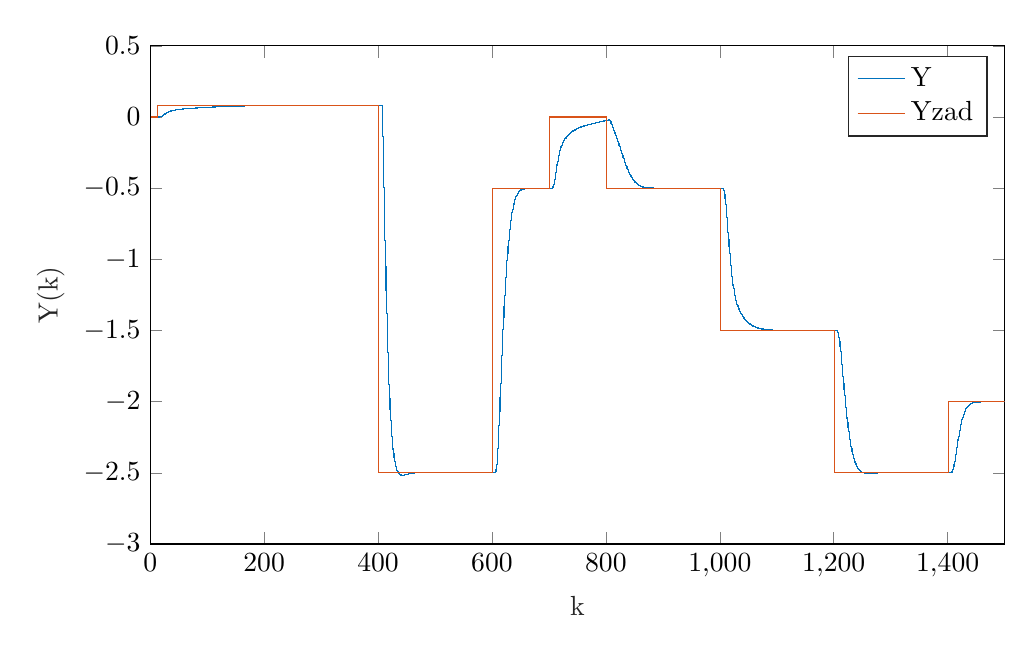
\begin{tikzpicture}

\begin{axis}[%
width=4.272in,
height=2.491in,
at={(0.717in,0.423in)},
scale only axis,
xmin=0,
xmax=1500,
xlabel style={font=\color{white!15!black}},
xlabel={k},
ymin=-3,
ymax=0.5,
ylabel style={font=\color{white!15!black}},
ylabel={Y(k)},
axis background/.style={fill=white},
legend style={legend cell align=left, align=left, draw=white!15!black}
]
\addplot[const plot, color=mycolor1] table[row sep=crcr] {%
1	0\\
2	0\\
3	0\\
4	0\\
5	0\\
6	0\\
7	0\\
8	0\\
9	0\\
10	0\\
11	0\\
12	0\\
13	0\\
14	0\\
15	0\\
16	0\\
17	0.000429996926167517\\
18	0.00167985740725402\\
19	0.00369161669830539\\
20	0.00624334429581961\\
21	0.00910107194892881\\
22	0.0120804183379811\\
23	0.0150572919098209\\
24	0.0179566613878681\\
25	0.0207363309151802\\
26	0.0233739713062449\\
27	0.0258590134174841\\
28	0.028188194979441\\
29	0.0303631483553462\\
30	0.0323889239310204\\
31	0.0342729124700211\\
32	0.0360239820432326\\
33	0.0376517901749899\\
34	0.0391662622286251\\
35	0.0405771701426304\\
36	0.0418914493199736\\
37	0.0431072855490408\\
38	0.044225981456863\\
39	0.0452533146435123\\
40	0.0461977707326047\\
41	0.0470686520235392\\
42	0.0478748942231733\\
43	0.0486245778315247\\
44	0.0493248061298936\\
45	0.0499817325456412\\
46	0.0506006409193173\\
47	0.0511860434326962\\
48	0.0517417827033034\\
49	0.0522711305571578\\
50	0.0527768783977767\\
51	0.0532614163028373\\
52	0.053726800031781\\
53	0.0541748065859623\\
54	0.0546069797269733\\
55	0.0550246670906494\\
56	0.0554290504574382\\
57	0.0558211705288142\\
58	0.0562019473176092\\
59	0.0565721970364786\\
60	0.0569326461804185\\
61	0.0572839433480791\\
62	0.0576266692282979\\
63	0.0579613450868302\\
64	0.0582884400179651\\
65	0.0586083771716727\\
66	0.0589215391252465\\
67	0.0592282725360511\\
68	0.0595288921866901\\
69	0.0598236845139663\\
70	0.060112910697145\\
71	0.0603968093683216\\
72	0.0606755989974221\\
73	0.0609494799960096\\
74	0.0612186365772249\\
75	0.0614832384035505\\
76	0.0617434420494128\\
77	0.0619993923017452\\
78	0.0622513384262049\\
79	0.0625003602048385\\
80	0.0627476297726911\\
81	0.0629938832885843\\
82	0.0632395029946593\\
83	0.0634846647177485\\
84	0.0637294379188122\\
85	0.0639738354593597\\
86	0.0642178360963839\\
87	0.0644613965169039\\
88	0.0647044591110565\\
89	0.0649469572882927\\
90	0.065188818996315\\
91	0.065429968919357\\
92	0.0656703297863773\\
93	0.0659098231365787\\
94	0.0661483697841481\\
95	0.0663858901306428\\
96	0.0666223044067116\\
97	0.0668575328837458\\
98	0.067091496073519\\
99	0.0673241149227332\\
100	0.0675553110044102\\
101	0.0677850067060963\\
102	0.0680131254141765\\
103	0.0682395916934405\\
104	0.0684643314610563\\
105	0.0686872721541627\\
106	0.0689083428903673\\
107	0.0691274746205024\\
108	0.0693446002730619\\
109	0.0695596548898141\\
110	0.0697725757521554\\
111	0.069983302497844\\
112	0.0701917772278242\\
113	0.070397944602923\\
114	0.070601751930269\\
115	0.0708031492393518\\
116	0.0710020893477023\\
117	0.0711985279162362\\
118	0.0713924234943605\\
119	0.0715837375549953\\
120	0.0717724345197136\\
121	0.071958481774249\\
122	0.072141849674659\\
123	0.0723225115444723\\
124	0.0725004436631794\\
125	0.0726756252464546\\
126	0.0728480384185228\\
127	0.0730176681771031\\
128	0.0731845023513795\\
129	0.0733485315534584\\
130	0.0735097491237862\\
131	0.0736681510709989\\
132	0.0738237360066844\\
133	0.0739765050755326\\
134	0.0741264618813462\\
135	0.0742736124093783\\
136	0.0744179649454553\\
137	0.0745595299923304\\
138	0.074698320183703\\
139	0.0748343501963225\\
140	0.0749676366605806\\
141	0.0750981980699793\\
142	0.0752260546898417\\
143	0.0753512284656179\\
144	0.0754737429311139\\
145	0.0755936231169554\\
146	0.0757108954595765\\
147	0.0758255877110027\\
148	0.075937728849679\\
149	0.0760473489925713\\
150	0.0761544793087519\\
151	0.0762591519346575\\
152	0.0763613998911926\\
153	0.0764612570028291\\
154	0.0765587578188369\\
155	0.0766539375367628\\
156	0.0767468319282573\\
157	0.0768374772673343\\
158	0.076925910261134\\
159	0.0770121679832415\\
160	0.0770962878096061\\
161	0.0771783073570871\\
162	0.0772582644246457\\
163	0.0773361969371879\\
164	0.0774121428920546\\
165	0.0774861403081455\\
166	0.0775582271776558\\
167	0.0776284414203938\\
168	0.0776968208406456\\
169	0.0777634030865407\\
170	0.0778282252757303\\
171	0.0778913072473396\\
172	0.0779526468897218\\
173	0.078012258975122\\
174	0.0780701723972097\\
175	0.0781264237113347\\
176	0.0781810529647701\\
177	0.0782341017193004\\
178	0.07828561221541\\
179	0.0783356268104193\\
180	0.0783841875325983\\
181	0.0784313357566664\\
182	0.0784771119957375\\
183	0.0785215557842994\\
184	0.0785647056227813\\
185	0.0786065989599469\\
186	0.0786472721969945\\
187	0.0786867607034529\\
188	0.0787250988391394\\
189	0.0787623199789889\\
190	0.0787984565390288\\
191	0.0788335400025895\\
192	0.0788676009462789\\
193	0.0789006690654887\\
194	0.0789327731993204\\
195	0.0789639413548837\\
196	0.0789942007309535\\
197	0.0790235777409852\\
198	0.0790520980354993\\
199	0.0790797865238464\\
200	0.0791066673953682\\
201	0.0791327641399695\\
202	0.0791580995681157\\
203	0.0791826958302725\\
204	0.0792065744358003\\
205	0.0792297562713203\\
206	0.0792522616185645\\
207	0.0792741101717244\\
208	0.0792953210543116\\
209	0.079315912835544\\
210	0.0793359035462696\\
211	0.0793553106944407\\
212	0.0793741512801516\\
213	0.0793924418102505\\
214	0.0794101983125376\\
215	0.0794274363495614\\
216	0.0794441710320233\\
217	0.0794604170318018\\
218	0.0794761885946067\\
219	0.0794914995522735\\
220	0.0795063633347073\\
221	0.0795207929814876\\
222	0.0795348011531414\\
223	0.0795484001420953\\
224	0.079561601883314\\
225	0.0795744179646365\\
226	0.0795868596368152\\
227	0.079598937823269\\
228	0.0796106631295566\\
229	0.0796220458525783\\
230	0.079633095989515\\
231	0.07964382324651\\
232	0.0796542370471017\\
233	0.079664346540415\\
234	0.0796741606091166\\
235	0.079683687877142\\
236	0.0796929367172002\\
237	0.079701915258063\\
238	0.0797106313916434\\
239	0.0797190927798714\\
240	0.079727306861371\\
241	0.0797352808579449\\
242	0.0797430217808724\\
243	0.0797505364370253\\
244	0.0797578314348076\\
245	0.0797649131899237\\
246	0.0797717879309798\\
247	0.0797784617049236\\
248	0.0797849403823271\\
249	0.0797912296625159\\
250	0.0797973350785512\\
251	0.0798032620020666\\
252	0.0798090156479656\\
253	0.0798146010789829\\
254	0.0798200232101139\\
255	0.0798252868129152\\
256	0.0798303965196814\\
257	0.0798353568275001\\
258	0.0798401721021895\\
259	0.0798448465821225\\
260	0.0798493843819386\\
261	0.0798537894961496\\
262	0.0798580658026392\\
263	0.0798622170660621\\
264	0.0798662469411442\\
265	0.0798701589758864\\
266	0.0798739566146759\\
267	0.0798776432013071\\
268	0.0798812219819145\\
269	0.0798846961078203\\
270	0.0798880686382996\\
271	0.0798913425432647\\
272	0.0798945207058721\\
273	0.0798976059250524\\
274	0.0799006009179682\\
275	0.0799035083223994\\
276	0.0799063306990591\\
277	0.0799090705338428\\
278	0.0799117302400116\\
279	0.0799143121603116\\
280	0.0799168185690325\\
281	0.0799192516740055\\
282	0.079921613618543\\
283	0.0799239064833223\\
284	0.079926132288214\\
285	0.0799282929940573\\
286	0.0799303905043835\\
287	0.0799324266670895\\
288	0.0799344032760621\\
289	0.0799363220727555\\
290	0.0799381847477222\\
291	0.0799399929420997\\
292	0.0799417482490539\\
293	0.0799434522151799\\
294	0.0799451063418627\\
295	0.0799467120865975\\
296	0.0799482708642719\\
297	0.0799497840484106\\
298	0.0799512529723839\\
299	0.0799526789305806\\
300	0.0799540631795471\\
301	0.0799554069390928\\
302	0.079956711393364\\
303	0.0799579776918855\\
304	0.0799592069505723\\
305	0.0799604002527121\\
306	0.0799615586499185\\
307	0.0799626831630564\\
308	0.0799637747831411\\
309	0.0799648344722105\\
310	0.0799658631641719\\
311	0.079966861765624\\
312	0.0799678311566556\\
313	0.0799687721916199\\
314	0.0799696856998872\\
315	0.0799705724865747\\
316	0.0799714333332558\\
317	0.0799722689986483\\
318	0.0799730802192821\\
319	0.0799738677101485\\
320	0.0799746321653293\\
321	0.0799753742586081\\
322	0.0799760946440641\\
323	0.0799767939566479\\
324	0.0799774728127406\\
325	0.0799781318106971\\
326	0.0799787715313726\\
327	0.0799793925386349\\
328	0.0799799953798605\\
329	0.0799805805864171\\
330	0.0799811486741314\\
331	0.0799817001437441\\
332	0.0799822354813501\\
333	0.0799827551588275\\
334	0.0799832596342532\\
335	0.0799837493523062\\
336	0.0799842247446593\\
337	0.0799846862303599\\
338	0.0799851342161989\\
339	0.0799855690970688\\
340	0.0799859912563124\\
341	0.07998640106606\\
342	0.0799867988875571\\
343	0.0799871850714834\\
344	0.0799875599582612\\
345	0.0799879238783558\\
346	0.0799882771525663\\
347	0.0799886200923086\\
348	0.0799889529998895\\
349	0.0799892761687734\\
350	0.0799895898838408\\
351	0.0799898944216394\\
352	0.0799901900506275\\
353	0.0799904770314111\\
354	0.0799907556169732\\
355	0.0799910260528966\\
356	0.079991288577581\\
357	0.0799915434224522\\
358	0.079991790812167\\
359	0.0799920309648102\\
360	0.0799922640920877\\
361	0.0799924903995125\\
362	0.0799927100865862\\
363	0.0799929233469744\\
364	0.079993130368678\\
365	0.0799933313341982\\
366	0.0799935264206978\\
367	0.0799937158001574\\
368	0.0799938996395267\\
369	0.0799940781008716\\
370	0.0799942513415176\\
371	0.0799944195141877\\
372	0.0799945827671377\\
373	0.0799947412442863\\
374	0.0799948950853425\\
375	0.0799950444259282\\
376	0.0799951893976983\\
377	0.0799953301284561\\
378	0.0799954667422665\\
379	0.0799955993595654\\
380	0.0799957280972652\\
381	0.0799958530688585\\
382	0.0799959743845179\\
383	0.079996092151193\\
384	0.0799962064727051\\
385	0.0799963174498381\\
386	0.0799964251804279\\
387	0.0799965297594481\\
388	0.0799966312790945\\
389	0.0799967298288653\\
390	0.079996825495641\\
391	0.0799969183637605\\
392	0.0799970085150954\\
393	0.0799970960291224\\
394	0.0799971809829931\\
395	0.0799972634516022\\
396	0.0799973435076536\\
397	0.0799974212217242\\
398	0.0799974966623264\\
399	0.0799975698959683\\
400	0.0799976409872123\\
401	0.0799977099987324\\
402	0.0799977769913688\\
403	0.0799978420241823\\
404	0.0799979051545056\\
405	0.0799979664379944\\
406	0.0834611234022582\\
407	0.000445377669206858\\
408	-0.137702549060071\\
409	-0.307791499035276\\
410	-0.493317939785426\\
411	-0.683246291067488\\
412	-0.870452699322663\\
413	-1.05038639135407\\
414	-1.22019230833832\\
415	-1.37815309639096\\
416	-1.52333893861367\\
417	-1.65538534095017\\
418	-1.77434599596453\\
419	-1.88058810870673\\
420	-1.9747115006762\\
421	-2.05748176336685\\
422	-2.12977306510395\\
423	-2.19251906844098\\
424	-2.2466716819272\\
425	-2.29316770504926\\
426	-2.33289791383202\\
427	-2.36668815931855\\
428	-2.39529036374816\\
429	-2.41937971301585\\
430	-2.43955615180992\\
431	-2.45634864014395\\
432	-2.47022116870909\\
433	-2.4815796204967\\
434	-2.49077873306118\\
435	-2.49812866202745\\
436	-2.50390086303397\\
437	-2.50833317854205\\
438	-2.51163413404806\\
439	-2.51398652023294\\
440	-2.5155503727197\\
441	-2.51646546967654\\
442	-2.51685345901222\\
443	-2.51681970917675\\
444	-2.51645495642791\\
445	-2.51583680076307\\
446	-2.51503108863983\\
447	-2.51409320029776\\
448	-2.5130692490467\\
449	-2.51199719502945\\
450	-2.51090787356622\\
451	-2.50982593772754\\
452	-2.50877071531297\\
453	-2.50775698159441\\
454	-2.50679565057803\\
455	-2.50589438881068\\
456	-2.50505815673338\\
457	-2.5042896832056\\
458	-2.50358987910365\\
459	-2.50295819589132\\
460	-2.5023929348453\\
461	-2.50189151226509\\
462	-2.50145068557266\\
463	-2.50106674475891\\
464	-2.50073567319744\\
465	-2.50045328144065\\
466	-2.50021531724548\\
467	-2.50001755475461\\
468	-2.49985586547693\\
469	-2.49972627346159\\
470	-2.49962499683573\\
471	-2.49954847767151\\
472	-2.4994934019581\\
473	-2.49945671127636\\
474	-2.49943560760599\\
475	-2.49942755253546\\
476	-2.49943026199517\\
477	-2.4994416974931\\
478	-2.49946005470142\\
479	-2.49948375012116\\
480	-2.49951140644213\\
481	-2.49954183711538\\
482	-2.4995740305662\\
483	-2.49960713439697\\
484	-2.49964043985942\\
485	-2.49967336681585\\
486	-2.49970544935669\\
487	-2.49973632219711\\
488	-2.49976570793808\\
489	-2.49979340524524\\
490	-2.49981927797282\\
491	-2.49984324523842\\
492	-2.49986527243668\\
493	-2.4998853631665\\
494	-2.49990355203529\\
495	-2.49991989829611\\
496	-2.49993448026766\\
497	-2.49994739048318\\
498	-2.4999587315125\\
499	-2.49996861240038\\
500	-2.49997714566475\\
501	-2.4999844447998\\
502	-2.49999062223051\\
503	-2.49999578766797\\
504	-2.5000000468175\\
505	-2.50000350039479\\
506	-2.50000624340857\\
507	-2.50000836467167\\
508	-2.50000994650569\\
509	-2.50001106460781\\
510	-2.50001178805159\\
511	-2.50001217939654\\
512	-2.50001229488422\\
513	-2.50001218470154\\
514	-2.50001189329406\\
515	-2.50001145971501\\
516	-2.50001091799741\\
517	-2.50001029753879\\
518	-2.50000962348997\\
519	-2.50000891714058\\
520	-2.50000819629566\\
521	-2.50000747563874\\
522	-2.50000676707809\\
523	-2.50000608007347\\
524	-2.50000542194169\\
525	-2.50000479814001\\
526	-2.50000421252676\\
527	-2.50000366759928\\
528	-2.50000316470947\\
529	-2.50000270425756\\
530	-2.50000228586515\\
531	-2.5000019085284\\
532	-2.50000157075272\\
533	-2.50000127067015\\
534	-2.50000100614075\\
535	-2.50000077483937\\
536	-2.50000057432913\\
537	-2.50000040212288\\
538	-2.50000025573385\\
539	-2.50000013271678\\
540	-2.50000003070061\\
541	-2.49999994741374\\
542	-2.49999988070287\\
543	-2.4999998285464\\
544	-2.49999978906299\\
545	-2.49999976051632\\
546	-2.49999974131647\\
547	-2.49999973001861\\
548	-2.49999972531959\\
549	-2.49999972605278\\
550	-2.49999973118165\\
551	-2.49999973979235\\
552	-2.49999975108577\\
553	-2.49999976436906\\
554	-2.49999977904713\\
555	-2.499999794614\\
556	-2.49999981064441\\
557	-2.49999982678563\\
558	-2.4999998427496\\
559	-2.49999985830554\\
560	-2.49999987327292\\
561	-2.49999988751501\\
562	-2.49999990093288\\
563	-2.49999991345989\\
564	-2.4999999250567\\
565	-2.49999993570681\\
566	-2.49999994541248\\
567	-2.49999995419119\\
568	-2.49999996207245\\
569	-2.49999996909508\\
570	-2.49999997530478\\
571	-2.49999998075207\\
572	-2.49999998549059\\
573	-2.49999998957558\\
574	-2.49999999306267\\
575	-2.49999999600692\\
576	-2.49999999846197\\
577	-2.50000000047945\\
578	-2.50000000210849\\
579	-2.50000000339538\\
580	-2.50000000438336\\
581	-2.50000000511245\\
582	-2.5000000056194\\
583	-2.50000000593772\\
584	-2.50000000609772\\
585	-2.50000000612661\\
586	-2.50000000604864\\
587	-2.50000000588525\\
588	-2.50000000565526\\
589	-2.50000000537503\\
590	-2.50000000505869\\
591	-2.50000000471827\\
592	-2.50000000436395\\
593	-2.50000000400423\\
594	-2.50000000364606\\
595	-2.5000000032951\\
596	-2.50000000295579\\
597	-2.50000000263154\\
598	-2.50000000232489\\
599	-2.50000000203759\\
600	-2.50000000177074\\
601	-2.50000000152492\\
602	-2.50000000130021\\
603	-2.50000000109636\\
604	-2.50000000091282\\
605	-2.50000000074878\\
606	-2.49366829040706\\
607	-2.47521677568716\\
608	-2.4417707812636\\
609	-2.39264551540685\\
610	-2.32873441369096\\
611	-2.25199195871997\\
612	-2.16500536276633\\
613	-2.07065108610891\\
614	-1.971829984075\\
615	-1.87127317706512\\
616	-1.77140967804628\\
617	-1.6742139190477\\
618	-1.58098577646836\\
619	-1.49245587824513\\
620	-1.40895633971766\\
621	-1.33055639972601\\
622	-1.25716414823541\\
623	-1.1885991328399\\
624	-1.12464171549476\\
625	-1.06506459254239\\
626	-1.00965343783689\\
627	-0.958215072674145\\
628	-0.910577862327263\\
629	-0.866588062637411\\
630	-0.826104208545526\\
631	-0.788990983392529\\
632	-0.755113543170917\\
633	-0.724332923269112\\
634	-0.696502875179218\\
635	-0.671468245677541\\
636	-0.649064820112673\\
637	-0.629120410894229\\
638	-0.611456886441852\\
639	-0.595892802906782\\
640	-0.582246312668839\\
641	-0.570338067482095\\
642	-0.559993896482801\\
643	-0.551047107689244\\
644	-0.543340326686428\\
645	-0.536726841761837\\
646	-0.53107146754826\\
647	-0.526250969841522\\
648	-0.522154112442252\\
649	-0.518681395184634\\
650	-0.515744553326294\\
651	-0.513265884404554\\
652	-0.511177461452538\\
653	-0.509420282646754\\
654	-0.507943398159695\\
655	-0.506703045997162\\
656	-0.505661820401432\\
657	-0.504787889265396\\
658	-0.504054271033047\\
659	-0.503438176749199\\
660	-0.502920419184219\\
661	-0.502484888175082\\
662	-0.502118089350501\\
663	-0.501808742101137\\
664	-0.501547431879436\\
665	-0.501326311544854\\
666	-0.501138846403744\\
667	-0.500979597740637\\
668	-0.500844039928396\\
669	-0.500728406583447\\
670	-0.500629561656997\\
671	-0.500544891792919\\
672	-0.500472216716254\\
673	-0.500409714828428\\
674	-0.500355861567287\\
675	-0.500309378437239\\
676	-0.500269190925022\\
677	-0.500234393790467\\
678	-0.500204222460365\\
679	-0.500178029460014\\
680	-0.500155264993811\\
681	-0.500135460936833\\
682	-0.500118217626514\\
683	-0.500103192950533\\
684	-0.500090093316437\\
685	-0.500078666162994\\
686	-0.500068693734944\\
687	-0.500059987893757\\
688	-0.500052385778879\\
689	-0.500045746168297\\
690	-0.500039946415263\\
691	-0.500034879860944\\
692	-0.500030453641291\\
693	-0.500026586821531\\
694	-0.500023208803918\\
695	-0.500020257964239\\
696	-0.500017680480584\\
697	-0.500015429324373\\
698	-0.500013463388848\\
699	-0.500011746734504\\
700	-0.500010247934364\\
701	-0.500008939504818\\
702	-0.500007797410042\\
703	-0.500006800629878\\
704	-0.500005930782605\\
705	-0.500005171795321\\
706	-0.497325367756597\\
707	-0.489869963037844\\
708	-0.477063622180696\\
709	-0.459364523990779\\
710	-0.437816454863775\\
711	-0.413692797186072\\
712	-0.388252525738122\\
713	-0.36259671297956\\
714	-0.337601637133882\\
715	-0.31390356432318\\
716	-0.291914682677989\\
717	-0.271855362357191\\
718	-0.253792920895732\\
719	-0.237680783881735\\
720	-0.223394447144512\\
721	-0.210762299817496\\
722	-0.199590466776133\\
723	-0.18968157869808\\
724	-0.180847888581611\\
725	-0.172919479200443\\
726	-0.165748462211434\\
727	-0.159210140523512\\
728	-0.153202098166517\\
729	-0.147641990675972\\
730	-0.1424646530931\\
731	-0.137619005530907\\
732	-0.13306509328138\\
733	-0.128771467995821\\
734	-0.124713009112803\\
735	-0.120869204788103\\
736	-0.117222858759374\\
737	-0.1137591602595\\
738	-0.110465042987787\\
739	-0.107328760600373\\
740	-0.104339615082568\\
741	-0.101487786653762\\
742	-0.098764226663059\\
743	-0.0961605865024587\\
744	-0.093669165029585\\
745	-0.0912828641264233\\
746	-0.0889951469935442\\
747	-0.0867999969627473\\
748	-0.0846918764407431\\
749	-0.0826656864841836\\
750	-0.0807167277952811\\
751	-0.0788406638793786\\
752	-0.0770334869032309\\
753	-0.0752914865498241\\
754	-0.073611221945615\\
755	-0.0719894965671817\\
756	-0.07042333592245\\
757	-0.0689099677407989\\
758	-0.0674468043851169\\
759	-0.0660314272049963\\
760	-0.0646615725728229\\
761	-0.0633351193750335\\
762	-0.0620500777633276\\
763	-0.0608045790014254\\
764	-0.0595968662701266\\
765	-0.0584252863162444\\
766	-0.0572882818495452\\
767	-0.0561843846066177\\
768	-0.0551122090122959\\
769	-0.0540704463785354\\
770	-0.0530578595880938\\
771	-0.052073278216466\\
772	-0.0511155940506345\\
773	-0.0501794454518762\\
774	-0.0492560759186547\\
775	-0.0483368536481953\\
776	-0.0474149875720553\\
777	-0.0464859291734736\\
778	-0.045547127224239\\
779	-0.0445975628631968\\
780	-0.0436372864247734\\
781	-0.0426670425251607\\
782	-0.0416879992127155\\
783	-0.0407015667080356\\
784	-0.0397092828783569\\
785	-0.0387127441704099\\
786	-0.0377135655541588\\
787	-0.0367133579545263\\
788	-0.0357137155719732\\
789	-0.034716208294015\\
790	-0.0337223762998869\\
791	-0.0327337252240211\\
792	-0.0317517210751334\\
793	-0.0307777846414014\\
794	-0.02981328543471\\
795	-0.0288595353976152\\
796	-0.02791778266114\\
797	-0.0269892056370252\\
798	-0.0260749076845785\\
799	-0.0251759125321528\\
800	-0.0242931605712489\\
801	-0.0234275060856604\\
802	-0.0225797154327952\\
803	-0.0217504661599412\\
804	-0.0209403470135147\\
805	-0.0201498587822173\\
806	-0.0218617895198858\\
807	-0.0274097494396049\\
808	-0.0356130688272596\\
809	-0.0452080555250375\\
810	-0.0554337603734492\\
811	-0.0658797928964488\\
812	-0.0763593178517146\\
813	-0.0868178620282841\\
814	-0.0972732447946698\\
815	-0.107776499102605\\
816	-0.118386825172685\\
817	-0.129156495574769\\
818	-0.140122968784201\\
819	-0.151306085695181\\
820	-0.162708586977475\\
821	-0.17431851446951\\
822	-0.186112405117313\\
823	-0.198058533115123\\
824	-0.210119766926611\\
825	-0.222255853701435\\
826	-0.234425130999023\\
827	-0.246585739812144\\
828	-0.258696402168285\\
829	-0.270716907740463\\
830	-0.282608443856022\\
831	-0.294333852376334\\
832	-0.305857858291019\\
833	-0.317147288430512\\
834	-0.328171282866293\\
835	-0.338901493654334\\
836	-0.349312262924702\\
837	-0.359380772734152\\
838	-0.369087160925883\\
839	-0.378414599421663\\
840	-0.387349333355345\\
841	-0.395880681043527\\
842	-0.404000995977541\\
843	-0.411705592893275\\
844	-0.418992640626209\\
845	-0.425863024961925\\
846	-0.432320185090215\\
847	-0.438369927581397\\
848	-0.444019229090294\\
849	-0.449275919727355\\
850	-0.454149369042772\\
851	-0.458650945038974\\
852	-0.462794056821091\\
853	-0.466593947347135\\
854	-0.47006736001154\\
855	-0.473232158778604\\
856	-0.476106948007918\\
857	-0.478710717101127\\
858	-0.481062522781695\\
859	-0.483181214715985\\
860	-0.485085206052879\\
861	-0.486792287965462\\
862	-0.488319485698774\\
863	-0.489682952606035\\
864	-0.490897898027388\\
865	-0.491978544548719\\
866	-0.492938110118368\\
867	-0.493788810644482\\
868	-0.494541878991592\\
869	-0.495207596689046\\
870	-0.495795335109392\\
871	-0.496313603334002\\
872	-0.496770100368698\\
873	-0.497171769785925\\
874	-0.497524855242464\\
875	-0.497834955648887\\
876	-0.498107079048904\\
877	-0.498345694505733\\
878	-0.498554781492462\\
879	-0.498737876448167\\
880	-0.498898116295617\\
881	-0.499038278823762\\
882	-0.49916081992254\\
883	-0.499267907722387\\
884	-0.499361453739173\\
885	-0.49944314116003\\
886	-0.499514450429072\\
887	-0.499576682306509\\
888	-0.499630978582076\\
889	-0.499678340625511\\
890	-0.499719645954443\\
891	-0.499755662994552\\
892	-0.499787064199148\\
893	-0.499814437686086\\
894	-0.499838297539788\\
895	-0.499859092915528\\
896	-0.499877216072327\\
897	-0.499893009450215\\
898	-0.499906771897245\\
899	-0.499918764141801\\
900	-0.499929213596405\\
901	-0.499938318570524\\
902	-0.499946251961796\\
903	-0.49995316448765\\
904	-0.499959187512541\\
905	-0.499964435519791\\
906	-0.499969008271501\\
907	-0.499972992694932\\
908	-0.499976464529265\\
909	-0.499979489762622\\
910	-0.499982125885618\\
911	-0.499984422984569\\
912	-0.499986424694599\\
913	-0.499988169030446\\
914	-0.499989689110503\\
915	-0.499991013787749\\
916	-0.499992168199447\\
917	-0.499993174246048\\
918	-0.499994051008365\\
919	-0.499994815110972\\
920	-0.499995481038732\\
921	-0.499996061412511\\
922	-0.49999656722932\\
923	-0.499997008071487\\
924	-0.49999739228885\\
925	-0.49999772715746\\
926	-0.499998019017809\\
927	-0.499998273395254\\
928	-0.499998495104903\\
929	-0.499998688343003\\
930	-0.499998856766542\\
931	-0.499999003562601\\
932	-0.499999131508783\\
933	-0.499999243025852\\
934	-0.499999340223608\\
935	-0.499999424940851\\
936	-0.499999498780204\\
937	-0.499999563138469\\
938	-0.499999619233059\\
939	-0.499999668125054\\
940	-0.499999710739273\\
941	-0.499999747881782\\
942	-0.499999780255145\\
943	-0.499999808471712\\
944	-0.49999983306521\\
945	-0.499999854500836\\
946	-0.499999873184055\\
947	-0.499999889468273\\
948	-0.499999903661522\\
949	-0.499999916032282\\
950	-0.499999926814561\\
951	-0.499999936212324\\
952	-0.499999944403344\\
953	-0.499999951542572\\
954	-0.499999957765062\\
955	-0.499999963188527\\
956	-0.499999967915567\\
957	-0.499999972035606\\
958	-0.499999975626588\\
959	-0.499999978756448\\
960	-0.499999981484397\\
961	-0.499999983862046\\
962	-0.499999985934376\\
963	-0.499999987740592\\
964	-0.499999989314867\\
965	-0.499999990686985\\
966	-0.499999991882905\\
967	-0.499999992925252\\
968	-0.499999993833748\\
969	-0.499999994625581\\
970	-0.499999995315732\\
971	-0.499999995917257\\
972	-0.499999996441539\\
973	-0.499999996898495\\
974	-0.499999997296772\\
975	-0.499999997643904\\
976	-0.49999999794646\\
977	-0.499999998210163\\
978	-0.499999998440003\\
979	-0.499999998640328\\
980	-0.499999998814929\\
981	-0.499999998967108\\
982	-0.499999999099746\\
983	-0.499999999215351\\
984	-0.49999999931611\\
985	-0.499999999403931\\
986	-0.499999999480475\\
987	-0.499999999547189\\
988	-0.499999999605336\\
989	-0.499999999656016\\
990	-0.499999999700189\\
991	-0.499999999738689\\
992	-0.499999999772245\\
993	-0.499999999801492\\
994	-0.499999999826983\\
995	-0.499999999849201\\
996	-0.499999999868565\\
997	-0.499999999885443\\
998	-0.499999999900154\\
999	-0.499999999912975\\
1000	-0.49999999992415\\
1001	-0.49999999993389\\
1002	-0.49999999994238\\
1003	-0.499999999949779\\
1004	-0.499999999956228\\
1005	-0.499999999961849\\
1006	-0.505162482154001\\
1007	-0.519130735227634\\
1008	-0.542713054779558\\
1009	-0.575135594342376\\
1010	-0.614851259218229\\
1011	-0.660041881167168\\
1012	-0.708906300834228\\
1013	-0.759807604276867\\
1014	-0.811336292770475\\
1015	-0.862327548072703\\
1016	-0.911855427839908\\
1017	-0.959216161233325\\
1018	-1.00390634208282\\
1019	-1.04559860405512\\
1020	-1.08411606900097\\
1021	-1.11940650237708\\
1022	-1.15151706792979\\
1023	-1.18057054103233\\
1024	-1.20674371705572\\
1025	-1.23024854603715\\
1026	-1.25131424126422\\
1027	-1.27017431162353\\
1028	-1.28705816437946\\
1029	-1.30219187202434\\
1030	-1.31579156566506\\
1031	-1.32805679051551\\
1032	-1.33916714075365\\
1033	-1.34928112950221\\
1034	-1.35853649467343\\
1035	-1.36705136656115\\
1036	-1.37492591203775\\
1037	-1.38224420454566\\
1038	-1.38907615925768\\
1039	-1.39547943235057\\
1040	-1.40150122220501\\
1041	-1.40717993558391\\
1042	-1.41254669833801\\
1043	-1.4176267011911\\
1044	-1.42244037873874\\
1045	-1.42700442520983\\
1046	-1.43133265597808\\
1047	-1.43543672424742\\
1048	-1.43932670431291\\
1049	-1.44301155477883\\
1050	-1.44649947623433\\
1051	-1.44979817830476\\
1052	-1.45291507077769\\
1053	-1.45585739275813\\
1054	-1.45863229268274\\
1055	-1.46124687063118\\
1056	-1.46370819282519\\
1057	-1.4660232866134\\
1058	-1.46819912269561\\
1059	-1.47024258991239\\
1060	-1.47216046665637\\
1061	-1.4739593918732\\
1062	-1.47564583771647\\
1063	-1.47722608519345\\
1064	-1.47870620357215\\
1065	-1.48009203389358\\
1066	-1.48138917662266\\
1067	-1.48260298325876\\
1068	-1.48373855158955\\
1069	-1.4848007241928\\
1070	-1.48579408975405\\
1071	-1.48672298676122\\
1072	-1.48759150915195\\
1073	-1.48840351351708\\
1074	-1.48916262749901\\
1075	-1.48987225906427\\
1076	-1.49053560636974\\
1077	-1.49115566798327\\
1078	-1.49173525325708\\
1079	-1.49227699268867\\
1080	-1.49278334813579\\
1081	-1.49325662278147\\
1082	-1.49369897076993\\
1083	-1.49411240645643\\
1084	-1.49449881323232\\
1085	-1.49485995190216\\
1086	-1.49519746860209\\
1087	-1.49551290225883\\
1088	-1.49580769159624\\
1089	-1.49608318170234\\
1090	-1.49634063017374\\
1091	-1.49658121285738\\
1092	-1.49680602921105\\
1093	-1.49701610730505\\
1094	-1.49721240848758\\
1095	-1.49739583173592\\
1096	-1.49756721771489\\
1097	-1.49772735256297\\
1098	-1.49787697142544\\
1099	-1.49801676175258\\
1100	-1.49814736637982\\
1101	-1.49826938640528\\
1102	-1.49838338387927\\
1103	-1.49848988431889\\
1104	-1.49858937905993\\
1105	-1.49868232745733\\
1106	-1.49876915894439\\
1107	-1.49885027496033\\
1108	-1.49892605075489\\
1109	-1.49899683707792\\
1110	-1.49906296176161\\
1111	-1.49912473120205\\
1112	-1.49918243174662\\
1113	-1.49923633099315\\
1114	-1.49928667900639\\
1115	-1.49933370945691\\
1116	-1.49937764068735\\
1117	-1.49941867671045\\
1118	-1.49945700814319\\
1119	-1.49949281308094\\
1120	-1.4995262579154\\
1121	-1.49955749809986\\
1122	-1.499586678865\\
1123	-1.49961393588844\\
1124	-1.49963939592084\\
1125	-1.49966317737139\\
1126	-1.49968539085521\\
1127	-1.49970613970509\\
1128	-1.49972552044988\\
1129	-1.49974362326158\\
1130	-1.49976053237332\\
1131	-1.49977632646983\\
1132	-1.49979107905246\\
1133	-1.49980485878021\\
1134	-1.49981772978839\\
1135	-1.49982975198639\\
1136	-1.49984098133587\\
1137	-1.49985147011066\\
1138	-1.49986126713963\\
1139	-1.49987041803352\\
1140	-1.49987896539693\\
1141	-1.49988694902627\\
1142	-1.4998944060948\\
1143	-1.49990137132537\\
1144	-1.49990787715189\\
1145	-1.49991395387013\\
1146	-1.49991962977859\\
1147	-1.49992493131012\\
1148	-1.49992988315481\\
1149	-1.49993450837491\\
1150	-1.49993882851203\\
1151	-1.49994286368741\\
1152	-1.49994663269553\\
1153	-1.49995015309153\\
1154	-1.49995344127293\\
1155	-1.49995651255592\\
1156	-1.49995938124667\\
1157	-1.49996206070786\\
1158	-1.49996456342096\\
1159	-1.49996690104424\\
1160	-1.49996908446712\\
1161	-1.49997112386082\\
1162	-1.49997302872572\\
1163	-1.49997480793564\\
1164	-1.49997646977907\\
1165	-1.49997802199785\\
1166	-1.49997947182318\\
1167	-1.4999808260093\\
1168	-1.49998209086495\\
1169	-1.49998327228274\\
1170	-1.4999843757666\\
1171	-1.49998540645743\\
1172	-1.49998636915702\\
1173	-1.49998726835042\\
1174	-1.49998810822684\\
1175	-1.49998889269916\\
1176	-1.49998962542215\\
1177	-1.49999030980951\\
1178	-1.49999094904975\\
1179	-1.49999154612105\\
1180	-1.49999210380515\\
1181	-1.49999262470027\\
1182	-1.49999311123326\\
1183	-1.49999356567088\\
1184	-1.49999399013035\\
1185	-1.49999438658925\\
1186	-1.49999475689467\\
1187	-1.49999510277191\\
1188	-1.4999954258324\\
1189	-1.49999572758131\\
1190	-1.4999960094245\\
1191	-1.4999962726751\\
1192	-1.49999651855963\\
1193	-1.49999674822366\\
1194	-1.49999696273724\\
1195	-1.49999716309979\\
1196	-1.49999735024483\\
1197	-1.49999752504429\\
1198	-1.49999768831257\\
1199	-1.49999784081037\\
1200	-1.49999798324818\\
1201	-1.49999811628964\\
1202	-1.49999824055462\\
1203	-1.49999835662207\\
1204	-1.49999846503277\\
1205	-1.49999856629181\\
1206	-1.50307978225187\\
1207	-1.51182084798439\\
1208	-1.52730976526972\\
1209	-1.54963309371281\\
1210	-1.57824606538645\\
1211	-1.61224555076249\\
1212	-1.65056479594256\\
1213	-1.69210635307625\\
1214	-1.73582758528768\\
1215	-1.78079083992854\\
1216	-1.82618815369887\\
1217	-1.87134832793273\\
1218	-1.91573244972252\\
1219	-1.958922444648\\
1220	-2.00060601652861\\
1221	-2.04056033547281\\
1222	-2.07863605042719\\
1223	-2.1147425985025\\
1224	-2.1488353331994\\
1225	-2.18090467118014\\
1226	-2.2109651630854\\
1227	-2.2390482041968\\
1228	-2.26519758504163\\
1229	-2.2894665625267\\
1230	-2.31191588722675\\
1231	-2.3326123952868\\
1232	-2.35162790791925\\
1233	-2.36903828209295\\
1234	-2.38492252717711\\
1235	-2.39936194979489\\
1236	-2.41243931845565\\
1237	-2.42423805555382\\
1238	-2.43484147115916\\
1239	-2.44433205396734\\
1240	-2.45279083233557\\
1241	-2.46029681429651\\
1242	-2.46692651103562\\
1243	-2.47275354427405\\
1244	-2.47784833470798\\
1245	-2.48227786625552\\
1246	-2.48610552079573\\
1247	-2.48939097488776\\
1248	-2.49219014960463\\
1249	-2.49455520545359\\
1250	-2.49653457527196\\
1251	-2.49817302894505\\
1252	-2.49951176466781\\
1253	-2.50058852220954\\
1254	-2.50143771423039\\
1255	-2.50209057215627\\
1256	-2.50257530347189\\
1257	-2.50291725757201\\
1258	-2.50313909754552\\
1259	-2.50326097547918\\
1260	-2.50330070907258\\
1261	-2.50327395756327\\
1262	-2.50319439517486\\
1263	-2.50307388052117\\
1264	-2.50292262062392\\
1265	-2.50274932842541\\
1266	-2.50256137289571\\
1267	-2.50236492104398\\
1268	-2.50216507134038\\
1269	-2.50196597823549\\
1270	-2.50177096762569\\
1271	-2.5015826432539\\
1272	-2.50140298415689\\
1273	-2.50123343337117\\
1274	-2.50107497819299\\
1275	-2.50092822235306\\
1276	-2.50079345051722\\
1277	-2.50067068556029\\
1278	-2.50055973908432\\
1279	-2.50046025566613\\
1280	-2.50037175132335\\
1281	-2.50029364668496\\
1282	-2.50022529534299\\
1283	-2.50016600784725\\
1284	-2.50011507178625\\
1285	-2.50007176837581\\
1286	-2.50003538595232\\
1287	-2.50000523074231\\
1288	-2.49998063525291\\
1289	-2.49996096460095\\
1290	-2.4999456210715\\
1291	-2.49993404716988\\
1292	-2.49992572740568\\
1293	-2.49992018902255\\
1294	-2.49991700186399\\
1295	-2.49991577754323\\
1296	-2.49991616806491\\
1297	-2.49991786402665\\
1298	-2.49992059251154\\
1299	-2.49992411476614\\
1300	-2.49992822374421\\
1301	-2.4999327415832\\
1302	-2.49993751706889\\
1303	-2.49994242313314\\
1304	-2.49994735442057\\
1305	-2.49995222495195\\
1306	-2.49995696590525\\
1307	-2.49996152352919\\
1308	-2.49996585719923\\
1309	-2.49996993762152\\
1310	-2.49997374518688\\
1311	-2.49997726847396\\
1312	-2.49998050289832\\
1313	-2.49998344950253\\
1314	-2.49998611388062\\
1315	-2.49998850522967\\
1316	-2.49999063552016\\
1317	-2.49999251877656\\
1318	-2.49999417045936\\
1319	-2.49999560693954\\
1320	-2.49999684505701\\
1321	-2.49999790175427\\
1322	-2.49999879377742\\
1323	-2.49999953743663\\
1324	-2.50000014841893\\
1325	-2.50000064164653\\
1326	-2.50000103117443\\
1327	-2.50000133012165\\
1328	-2.5000015506309\\
1329	-2.5000017038519\\
1330	-2.50000179994435\\
1331	-2.50000184809658\\
1332	-2.50000185655683\\
1333	-2.50000183267414\\
1334	-2.50000178294636\\
1335	-2.50000171307322\\
1336	-2.50000162801261\\
1337	-2.50000153203842\\
1338	-2.50000142879891\\
1339	-2.5000013213743\\
1340	-2.50000121233299\\
1341	-2.5000011037856\\
1342	-2.50000099743636\\
1343	-2.50000089463161\\
1344	-2.50000079640501\\
1345	-2.5000007035194\\
1346	-2.50000061650531\\
1347	-2.50000053569594\\
1348	-2.50000046125891\\
1349	-2.50000039322472\\
1350	-2.50000033151209\\
1351	-2.50000027595041\\
1352	-2.50000022629942\\
1353	-2.50000018226629\\
1354	-2.50000014352045\\
1355	-2.50000010970612\\
1356	-2.50000008045298\\
1357	-2.50000005538505\\
1358	-2.50000003412798\\
1359	-2.50000001631494\\
1360	-2.50000000159124\\
1361	-2.49999998961799\\
1362	-2.49999998007465\\
1363	-2.49999997266093\\
1364	-2.4999999670979\\
1365	-2.49999996312862\\
1366	-2.49999996051822\\
1367	-2.49999995905362\\
1368	-2.49999995854299\\
1369	-2.49999995881485\\
1370	-2.49999995971714\\
1371	-2.49999996111602\\
1372	-2.49999996289468\\
1373	-2.49999996495206\\
1374	-2.49999996720154\\
1375	-2.49999996956966\\
1376	-2.49999997199484\\
1377	-2.49999997442618\\
1378	-2.49999997682228\\
1379	-2.49999997915011\\
1380	-2.49999998138403\\
1381	-2.49999998350477\\
1382	-2.49999998549858\\
1383	-2.49999998735638\\
1384	-2.49999998907308\\
1385	-2.49999999064688\\
1386	-2.49999999207868\\
1387	-2.49999999337155\\
1388	-2.49999999453031\\
1389	-2.49999999556106\\
1390	-2.49999999647088\\
1391	-2.49999999726752\\
1392	-2.49999999795915\\
1393	-2.49999999855412\\
1394	-2.49999999906081\\
1395	-2.49999999948748\\
1396	-2.49999999984216\\
1397	-2.50000000013257\\
1398	-2.500000000366\\
1399	-2.50000000054936\\
1400	-2.50000000068904\\
1401	-2.50000000079096\\
1402	-2.50000000086058\\
1403	-2.50000000090281\\
1404	-2.50000000092214\\
1405	-2.50000000092256\\
1406	-2.49844105576363\\
1407	-2.49392646647967\\
1408	-2.4857821906591\\
1409	-2.4738551387298\\
1410	-2.45835038222841\\
1411	-2.43970140368736\\
1412	-2.41846945006252\\
1413	-2.39526832393505\\
1414	-2.37071066981974\\
1415	-2.34537182614274\\
1416	-2.31976754879208\\
1417	-2.29434229648596\\
1418	-2.26946523428579\\
1419	-2.24543160377106\\
1420	-2.22246758529226\\
1421	-2.20073721191718\\
1422	-2.18035027087187\\
1423	-2.16137044061032\\
1424	-2.1438231610624\\
1425	-2.12770292639456\\
1426	-2.11298092145955\\
1427	-2.09961085549831\\
1428	-2.08753335989324\\
1429	-2.0766795347125\\
1430	-2.06697386604362\\
1431	-2.05833666454276\\
1432	-2.05068612284404\\
1433	-2.04394005293601\\
1434	-2.03801734150202\\
1435	-2.03283914815901\\
1436	-2.02832986545081\\
1437	-2.02441785779623\\
1438	-2.02103599736282\\
1439	-2.01812201659026\\
1440	-2.01561869886192\\
1441	-2.01347393005497\\
1442	-2.01164063412567\\
1443	-2.01007661545543\\
1444	-2.00874432948095\\
1445	-2.00761060131867\\
1446	-2.0066463091195\\
1447	-2.00582604765957\\
1448	-2.0051277852045\\
1449	-2.00453252391438\\
1450	-2.00402397155658\\
1451	-2.00358823008861\\
1452	-2.00321350481018\\
1453	-2.0028898362692\\
1454	-2.00260885591627\\
1455	-2.00236356559899\\
1456	-2.00214814032645\\
1457	-2.00195775327092\\
1458	-2.00178842166738\\
1459	-2.00163687208617\\
1460	-2.00150042346023\\
1461	-2.00137688622152\\
1462	-2.00126447592348\\
1463	-2.00116173978235\\
1464	-2.00106749464981\\
1465	-2.00098077502354\\
1466	-2.00090078980702\\
1467	-2.00082688663719\\
1468	-2.0007585227078\\
1469	-2.00069524112382\\
1470	-2.00063665192645\\
1471	-2.00058241702866\\
1472	-2.0005322383948\\
1473	-2.00048584888597\\
1474	-2.00044300527333\\
1475	-2.00040348299472\\
1476	-2.00036707229616\\
1477	-2.000333575458\\
1478	-2.00030280485721\\
1479	-2.00027458166225\\
1480	-2.0002487349952\\
1481	-2.00022510142934\\
1482	-2.0002035247178\\
1483	-2.00018385567242\\
1484	-2.00016595213122\\
1485	-2.00014967896862\\
1486	-2.00013490811542\\
1487	-2.00012151856571\\
1488	-2.00010939635583\\
1489	-2.00009843450697\\
1490	-2.00008853292747\\
1491	-2.00007959827441\\
1492	-2.00007154377672\\
1493	-2.00006428902345\\
1494	-2.00005775972208\\
1495	-2.00005188743228\\
1496	-2.00004660928049\\
1497	-2.0000418676609\\
1498	-2.00003760992793\\
1499	-2.00003378808481\\
1500	-2.00003035847254\\
};
\addlegendentry{Y}

\addplot[const plot, color=mycolor2] table[row sep=crcr] {%
1	0\\
2	0\\
3	0\\
4	0\\
5	0\\
6	0\\
7	0\\
8	0\\
9	0\\
10	0\\
11	0\\
12	0.08\\
13	0.08\\
14	0.08\\
15	0.08\\
16	0.08\\
17	0.08\\
18	0.08\\
19	0.08\\
20	0.08\\
21	0.08\\
22	0.08\\
23	0.08\\
24	0.08\\
25	0.08\\
26	0.08\\
27	0.08\\
28	0.08\\
29	0.08\\
30	0.08\\
31	0.08\\
32	0.08\\
33	0.08\\
34	0.08\\
35	0.08\\
36	0.08\\
37	0.08\\
38	0.08\\
39	0.08\\
40	0.08\\
41	0.08\\
42	0.08\\
43	0.08\\
44	0.08\\
45	0.08\\
46	0.08\\
47	0.08\\
48	0.08\\
49	0.08\\
50	0.08\\
51	0.08\\
52	0.08\\
53	0.08\\
54	0.08\\
55	0.08\\
56	0.08\\
57	0.08\\
58	0.08\\
59	0.08\\
60	0.08\\
61	0.08\\
62	0.08\\
63	0.08\\
64	0.08\\
65	0.08\\
66	0.08\\
67	0.08\\
68	0.08\\
69	0.08\\
70	0.08\\
71	0.08\\
72	0.08\\
73	0.08\\
74	0.08\\
75	0.08\\
76	0.08\\
77	0.08\\
78	0.08\\
79	0.08\\
80	0.08\\
81	0.08\\
82	0.08\\
83	0.08\\
84	0.08\\
85	0.08\\
86	0.08\\
87	0.08\\
88	0.08\\
89	0.08\\
90	0.08\\
91	0.08\\
92	0.08\\
93	0.08\\
94	0.08\\
95	0.08\\
96	0.08\\
97	0.08\\
98	0.08\\
99	0.08\\
100	0.08\\
101	0.08\\
102	0.08\\
103	0.08\\
104	0.08\\
105	0.08\\
106	0.08\\
107	0.08\\
108	0.08\\
109	0.08\\
110	0.08\\
111	0.08\\
112	0.08\\
113	0.08\\
114	0.08\\
115	0.08\\
116	0.08\\
117	0.08\\
118	0.08\\
119	0.08\\
120	0.08\\
121	0.08\\
122	0.08\\
123	0.08\\
124	0.08\\
125	0.08\\
126	0.08\\
127	0.08\\
128	0.08\\
129	0.08\\
130	0.08\\
131	0.08\\
132	0.08\\
133	0.08\\
134	0.08\\
135	0.08\\
136	0.08\\
137	0.08\\
138	0.08\\
139	0.08\\
140	0.08\\
141	0.08\\
142	0.08\\
143	0.08\\
144	0.08\\
145	0.08\\
146	0.08\\
147	0.08\\
148	0.08\\
149	0.08\\
150	0.08\\
151	0.08\\
152	0.08\\
153	0.08\\
154	0.08\\
155	0.08\\
156	0.08\\
157	0.08\\
158	0.08\\
159	0.08\\
160	0.08\\
161	0.08\\
162	0.08\\
163	0.08\\
164	0.08\\
165	0.08\\
166	0.08\\
167	0.08\\
168	0.08\\
169	0.08\\
170	0.08\\
171	0.08\\
172	0.08\\
173	0.08\\
174	0.08\\
175	0.08\\
176	0.08\\
177	0.08\\
178	0.08\\
179	0.08\\
180	0.08\\
181	0.08\\
182	0.08\\
183	0.08\\
184	0.08\\
185	0.08\\
186	0.08\\
187	0.08\\
188	0.08\\
189	0.08\\
190	0.08\\
191	0.08\\
192	0.08\\
193	0.08\\
194	0.08\\
195	0.08\\
196	0.08\\
197	0.08\\
198	0.08\\
199	0.08\\
200	0.08\\
201	0.08\\
202	0.08\\
203	0.08\\
204	0.08\\
205	0.08\\
206	0.08\\
207	0.08\\
208	0.08\\
209	0.08\\
210	0.08\\
211	0.08\\
212	0.08\\
213	0.08\\
214	0.08\\
215	0.08\\
216	0.08\\
217	0.08\\
218	0.08\\
219	0.08\\
220	0.08\\
221	0.08\\
222	0.08\\
223	0.08\\
224	0.08\\
225	0.08\\
226	0.08\\
227	0.08\\
228	0.08\\
229	0.08\\
230	0.08\\
231	0.08\\
232	0.08\\
233	0.08\\
234	0.08\\
235	0.08\\
236	0.08\\
237	0.08\\
238	0.08\\
239	0.08\\
240	0.08\\
241	0.08\\
242	0.08\\
243	0.08\\
244	0.08\\
245	0.08\\
246	0.08\\
247	0.08\\
248	0.08\\
249	0.08\\
250	0.08\\
251	0.08\\
252	0.08\\
253	0.08\\
254	0.08\\
255	0.08\\
256	0.08\\
257	0.08\\
258	0.08\\
259	0.08\\
260	0.08\\
261	0.08\\
262	0.08\\
263	0.08\\
264	0.08\\
265	0.08\\
266	0.08\\
267	0.08\\
268	0.08\\
269	0.08\\
270	0.08\\
271	0.08\\
272	0.08\\
273	0.08\\
274	0.08\\
275	0.08\\
276	0.08\\
277	0.08\\
278	0.08\\
279	0.08\\
280	0.08\\
281	0.08\\
282	0.08\\
283	0.08\\
284	0.08\\
285	0.08\\
286	0.08\\
287	0.08\\
288	0.08\\
289	0.08\\
290	0.08\\
291	0.08\\
292	0.08\\
293	0.08\\
294	0.08\\
295	0.08\\
296	0.08\\
297	0.08\\
298	0.08\\
299	0.08\\
300	0.08\\
301	0.08\\
302	0.08\\
303	0.08\\
304	0.08\\
305	0.08\\
306	0.08\\
307	0.08\\
308	0.08\\
309	0.08\\
310	0.08\\
311	0.08\\
312	0.08\\
313	0.08\\
314	0.08\\
315	0.08\\
316	0.08\\
317	0.08\\
318	0.08\\
319	0.08\\
320	0.08\\
321	0.08\\
322	0.08\\
323	0.08\\
324	0.08\\
325	0.08\\
326	0.08\\
327	0.08\\
328	0.08\\
329	0.08\\
330	0.08\\
331	0.08\\
332	0.08\\
333	0.08\\
334	0.08\\
335	0.08\\
336	0.08\\
337	0.08\\
338	0.08\\
339	0.08\\
340	0.08\\
341	0.08\\
342	0.08\\
343	0.08\\
344	0.08\\
345	0.08\\
346	0.08\\
347	0.08\\
348	0.08\\
349	0.08\\
350	0.08\\
351	0.08\\
352	0.08\\
353	0.08\\
354	0.08\\
355	0.08\\
356	0.08\\
357	0.08\\
358	0.08\\
359	0.08\\
360	0.08\\
361	0.08\\
362	0.08\\
363	0.08\\
364	0.08\\
365	0.08\\
366	0.08\\
367	0.08\\
368	0.08\\
369	0.08\\
370	0.08\\
371	0.08\\
372	0.08\\
373	0.08\\
374	0.08\\
375	0.08\\
376	0.08\\
377	0.08\\
378	0.08\\
379	0.08\\
380	0.08\\
381	0.08\\
382	0.08\\
383	0.08\\
384	0.08\\
385	0.08\\
386	0.08\\
387	0.08\\
388	0.08\\
389	0.08\\
390	0.08\\
391	0.08\\
392	0.08\\
393	0.08\\
394	0.08\\
395	0.08\\
396	0.08\\
397	0.08\\
398	0.08\\
399	0.08\\
400	0.08\\
401	-2.5\\
402	-2.5\\
403	-2.5\\
404	-2.5\\
405	-2.5\\
406	-2.5\\
407	-2.5\\
408	-2.5\\
409	-2.5\\
410	-2.5\\
411	-2.5\\
412	-2.5\\
413	-2.5\\
414	-2.5\\
415	-2.5\\
416	-2.5\\
417	-2.5\\
418	-2.5\\
419	-2.5\\
420	-2.5\\
421	-2.5\\
422	-2.5\\
423	-2.5\\
424	-2.5\\
425	-2.5\\
426	-2.5\\
427	-2.5\\
428	-2.5\\
429	-2.5\\
430	-2.5\\
431	-2.5\\
432	-2.5\\
433	-2.5\\
434	-2.5\\
435	-2.5\\
436	-2.5\\
437	-2.5\\
438	-2.5\\
439	-2.5\\
440	-2.5\\
441	-2.5\\
442	-2.5\\
443	-2.5\\
444	-2.5\\
445	-2.5\\
446	-2.5\\
447	-2.5\\
448	-2.5\\
449	-2.5\\
450	-2.5\\
451	-2.5\\
452	-2.5\\
453	-2.5\\
454	-2.5\\
455	-2.5\\
456	-2.5\\
457	-2.5\\
458	-2.5\\
459	-2.5\\
460	-2.5\\
461	-2.5\\
462	-2.5\\
463	-2.5\\
464	-2.5\\
465	-2.5\\
466	-2.5\\
467	-2.5\\
468	-2.5\\
469	-2.5\\
470	-2.5\\
471	-2.5\\
472	-2.5\\
473	-2.5\\
474	-2.5\\
475	-2.5\\
476	-2.5\\
477	-2.5\\
478	-2.5\\
479	-2.5\\
480	-2.5\\
481	-2.5\\
482	-2.5\\
483	-2.5\\
484	-2.5\\
485	-2.5\\
486	-2.5\\
487	-2.5\\
488	-2.5\\
489	-2.5\\
490	-2.5\\
491	-2.5\\
492	-2.5\\
493	-2.5\\
494	-2.5\\
495	-2.5\\
496	-2.5\\
497	-2.5\\
498	-2.5\\
499	-2.5\\
500	-2.5\\
501	-2.5\\
502	-2.5\\
503	-2.5\\
504	-2.5\\
505	-2.5\\
506	-2.5\\
507	-2.5\\
508	-2.5\\
509	-2.5\\
510	-2.5\\
511	-2.5\\
512	-2.5\\
513	-2.5\\
514	-2.5\\
515	-2.5\\
516	-2.5\\
517	-2.5\\
518	-2.5\\
519	-2.5\\
520	-2.5\\
521	-2.5\\
522	-2.5\\
523	-2.5\\
524	-2.5\\
525	-2.5\\
526	-2.5\\
527	-2.5\\
528	-2.5\\
529	-2.5\\
530	-2.5\\
531	-2.5\\
532	-2.5\\
533	-2.5\\
534	-2.5\\
535	-2.5\\
536	-2.5\\
537	-2.5\\
538	-2.5\\
539	-2.5\\
540	-2.5\\
541	-2.5\\
542	-2.5\\
543	-2.5\\
544	-2.5\\
545	-2.5\\
546	-2.5\\
547	-2.5\\
548	-2.5\\
549	-2.5\\
550	-2.5\\
551	-2.5\\
552	-2.5\\
553	-2.5\\
554	-2.5\\
555	-2.5\\
556	-2.5\\
557	-2.5\\
558	-2.5\\
559	-2.5\\
560	-2.5\\
561	-2.5\\
562	-2.5\\
563	-2.5\\
564	-2.5\\
565	-2.5\\
566	-2.5\\
567	-2.5\\
568	-2.5\\
569	-2.5\\
570	-2.5\\
571	-2.5\\
572	-2.5\\
573	-2.5\\
574	-2.5\\
575	-2.5\\
576	-2.5\\
577	-2.5\\
578	-2.5\\
579	-2.5\\
580	-2.5\\
581	-2.5\\
582	-2.5\\
583	-2.5\\
584	-2.5\\
585	-2.5\\
586	-2.5\\
587	-2.5\\
588	-2.5\\
589	-2.5\\
590	-2.5\\
591	-2.5\\
592	-2.5\\
593	-2.5\\
594	-2.5\\
595	-2.5\\
596	-2.5\\
597	-2.5\\
598	-2.5\\
599	-2.5\\
600	-2.5\\
601	-0.5\\
602	-0.5\\
603	-0.5\\
604	-0.5\\
605	-0.5\\
606	-0.5\\
607	-0.5\\
608	-0.5\\
609	-0.5\\
610	-0.5\\
611	-0.5\\
612	-0.5\\
613	-0.5\\
614	-0.5\\
615	-0.5\\
616	-0.5\\
617	-0.5\\
618	-0.5\\
619	-0.5\\
620	-0.5\\
621	-0.5\\
622	-0.5\\
623	-0.5\\
624	-0.5\\
625	-0.5\\
626	-0.5\\
627	-0.5\\
628	-0.5\\
629	-0.5\\
630	-0.5\\
631	-0.5\\
632	-0.5\\
633	-0.5\\
634	-0.5\\
635	-0.5\\
636	-0.5\\
637	-0.5\\
638	-0.5\\
639	-0.5\\
640	-0.5\\
641	-0.5\\
642	-0.5\\
643	-0.5\\
644	-0.5\\
645	-0.5\\
646	-0.5\\
647	-0.5\\
648	-0.5\\
649	-0.5\\
650	-0.5\\
651	-0.5\\
652	-0.5\\
653	-0.5\\
654	-0.5\\
655	-0.5\\
656	-0.5\\
657	-0.5\\
658	-0.5\\
659	-0.5\\
660	-0.5\\
661	-0.5\\
662	-0.5\\
663	-0.5\\
664	-0.5\\
665	-0.5\\
666	-0.5\\
667	-0.5\\
668	-0.5\\
669	-0.5\\
670	-0.5\\
671	-0.5\\
672	-0.5\\
673	-0.5\\
674	-0.5\\
675	-0.5\\
676	-0.5\\
677	-0.5\\
678	-0.5\\
679	-0.5\\
680	-0.5\\
681	-0.5\\
682	-0.5\\
683	-0.5\\
684	-0.5\\
685	-0.5\\
686	-0.5\\
687	-0.5\\
688	-0.5\\
689	-0.5\\
690	-0.5\\
691	-0.5\\
692	-0.5\\
693	-0.5\\
694	-0.5\\
695	-0.5\\
696	-0.5\\
697	-0.5\\
698	-0.5\\
699	-0.5\\
700	-0.5\\
701	0\\
702	0\\
703	0\\
704	0\\
705	0\\
706	0\\
707	0\\
708	0\\
709	0\\
710	0\\
711	0\\
712	0\\
713	0\\
714	0\\
715	0\\
716	0\\
717	0\\
718	0\\
719	0\\
720	0\\
721	0\\
722	0\\
723	0\\
724	0\\
725	0\\
726	0\\
727	0\\
728	0\\
729	0\\
730	0\\
731	0\\
732	0\\
733	0\\
734	0\\
735	0\\
736	0\\
737	0\\
738	0\\
739	0\\
740	0\\
741	0\\
742	0\\
743	0\\
744	0\\
745	0\\
746	0\\
747	0\\
748	0\\
749	0\\
750	0\\
751	0\\
752	0\\
753	0\\
754	0\\
755	0\\
756	0\\
757	0\\
758	0\\
759	0\\
760	0\\
761	0\\
762	0\\
763	0\\
764	0\\
765	0\\
766	0\\
767	0\\
768	0\\
769	0\\
770	0\\
771	0\\
772	0\\
773	0\\
774	0\\
775	0\\
776	0\\
777	0\\
778	0\\
779	0\\
780	0\\
781	0\\
782	0\\
783	0\\
784	0\\
785	0\\
786	0\\
787	0\\
788	0\\
789	0\\
790	0\\
791	0\\
792	0\\
793	0\\
794	0\\
795	0\\
796	0\\
797	0\\
798	0\\
799	0\\
800	0\\
801	-0.5\\
802	-0.5\\
803	-0.5\\
804	-0.5\\
805	-0.5\\
806	-0.5\\
807	-0.5\\
808	-0.5\\
809	-0.5\\
810	-0.5\\
811	-0.5\\
812	-0.5\\
813	-0.5\\
814	-0.5\\
815	-0.5\\
816	-0.5\\
817	-0.5\\
818	-0.5\\
819	-0.5\\
820	-0.5\\
821	-0.5\\
822	-0.5\\
823	-0.5\\
824	-0.5\\
825	-0.5\\
826	-0.5\\
827	-0.5\\
828	-0.5\\
829	-0.5\\
830	-0.5\\
831	-0.5\\
832	-0.5\\
833	-0.5\\
834	-0.5\\
835	-0.5\\
836	-0.5\\
837	-0.5\\
838	-0.5\\
839	-0.5\\
840	-0.5\\
841	-0.5\\
842	-0.5\\
843	-0.5\\
844	-0.5\\
845	-0.5\\
846	-0.5\\
847	-0.5\\
848	-0.5\\
849	-0.5\\
850	-0.5\\
851	-0.5\\
852	-0.5\\
853	-0.5\\
854	-0.5\\
855	-0.5\\
856	-0.5\\
857	-0.5\\
858	-0.5\\
859	-0.5\\
860	-0.5\\
861	-0.5\\
862	-0.5\\
863	-0.5\\
864	-0.5\\
865	-0.5\\
866	-0.5\\
867	-0.5\\
868	-0.5\\
869	-0.5\\
870	-0.5\\
871	-0.5\\
872	-0.5\\
873	-0.5\\
874	-0.5\\
875	-0.5\\
876	-0.5\\
877	-0.5\\
878	-0.5\\
879	-0.5\\
880	-0.5\\
881	-0.5\\
882	-0.5\\
883	-0.5\\
884	-0.5\\
885	-0.5\\
886	-0.5\\
887	-0.5\\
888	-0.5\\
889	-0.5\\
890	-0.5\\
891	-0.5\\
892	-0.5\\
893	-0.5\\
894	-0.5\\
895	-0.5\\
896	-0.5\\
897	-0.5\\
898	-0.5\\
899	-0.5\\
900	-0.5\\
901	-0.5\\
902	-0.5\\
903	-0.5\\
904	-0.5\\
905	-0.5\\
906	-0.5\\
907	-0.5\\
908	-0.5\\
909	-0.5\\
910	-0.5\\
911	-0.5\\
912	-0.5\\
913	-0.5\\
914	-0.5\\
915	-0.5\\
916	-0.5\\
917	-0.5\\
918	-0.5\\
919	-0.5\\
920	-0.5\\
921	-0.5\\
922	-0.5\\
923	-0.5\\
924	-0.5\\
925	-0.5\\
926	-0.5\\
927	-0.5\\
928	-0.5\\
929	-0.5\\
930	-0.5\\
931	-0.5\\
932	-0.5\\
933	-0.5\\
934	-0.5\\
935	-0.5\\
936	-0.5\\
937	-0.5\\
938	-0.5\\
939	-0.5\\
940	-0.5\\
941	-0.5\\
942	-0.5\\
943	-0.5\\
944	-0.5\\
945	-0.5\\
946	-0.5\\
947	-0.5\\
948	-0.5\\
949	-0.5\\
950	-0.5\\
951	-0.5\\
952	-0.5\\
953	-0.5\\
954	-0.5\\
955	-0.5\\
956	-0.5\\
957	-0.5\\
958	-0.5\\
959	-0.5\\
960	-0.5\\
961	-0.5\\
962	-0.5\\
963	-0.5\\
964	-0.5\\
965	-0.5\\
966	-0.5\\
967	-0.5\\
968	-0.5\\
969	-0.5\\
970	-0.5\\
971	-0.5\\
972	-0.5\\
973	-0.5\\
974	-0.5\\
975	-0.5\\
976	-0.5\\
977	-0.5\\
978	-0.5\\
979	-0.5\\
980	-0.5\\
981	-0.5\\
982	-0.5\\
983	-0.5\\
984	-0.5\\
985	-0.5\\
986	-0.5\\
987	-0.5\\
988	-0.5\\
989	-0.5\\
990	-0.5\\
991	-0.5\\
992	-0.5\\
993	-0.5\\
994	-0.5\\
995	-0.5\\
996	-0.5\\
997	-0.5\\
998	-0.5\\
999	-0.5\\
1000	-0.5\\
1001	-1.5\\
1002	-1.5\\
1003	-1.5\\
1004	-1.5\\
1005	-1.5\\
1006	-1.5\\
1007	-1.5\\
1008	-1.5\\
1009	-1.5\\
1010	-1.5\\
1011	-1.5\\
1012	-1.5\\
1013	-1.5\\
1014	-1.5\\
1015	-1.5\\
1016	-1.5\\
1017	-1.5\\
1018	-1.5\\
1019	-1.5\\
1020	-1.5\\
1021	-1.5\\
1022	-1.5\\
1023	-1.5\\
1024	-1.5\\
1025	-1.5\\
1026	-1.5\\
1027	-1.5\\
1028	-1.5\\
1029	-1.5\\
1030	-1.5\\
1031	-1.5\\
1032	-1.5\\
1033	-1.5\\
1034	-1.5\\
1035	-1.5\\
1036	-1.5\\
1037	-1.5\\
1038	-1.5\\
1039	-1.5\\
1040	-1.5\\
1041	-1.5\\
1042	-1.5\\
1043	-1.5\\
1044	-1.5\\
1045	-1.5\\
1046	-1.5\\
1047	-1.5\\
1048	-1.5\\
1049	-1.5\\
1050	-1.5\\
1051	-1.5\\
1052	-1.5\\
1053	-1.5\\
1054	-1.5\\
1055	-1.5\\
1056	-1.5\\
1057	-1.5\\
1058	-1.5\\
1059	-1.5\\
1060	-1.5\\
1061	-1.5\\
1062	-1.5\\
1063	-1.5\\
1064	-1.5\\
1065	-1.5\\
1066	-1.5\\
1067	-1.5\\
1068	-1.5\\
1069	-1.5\\
1070	-1.5\\
1071	-1.5\\
1072	-1.5\\
1073	-1.5\\
1074	-1.5\\
1075	-1.5\\
1076	-1.5\\
1077	-1.5\\
1078	-1.5\\
1079	-1.5\\
1080	-1.5\\
1081	-1.5\\
1082	-1.5\\
1083	-1.5\\
1084	-1.5\\
1085	-1.5\\
1086	-1.5\\
1087	-1.5\\
1088	-1.5\\
1089	-1.5\\
1090	-1.5\\
1091	-1.5\\
1092	-1.5\\
1093	-1.5\\
1094	-1.5\\
1095	-1.5\\
1096	-1.5\\
1097	-1.5\\
1098	-1.5\\
1099	-1.5\\
1100	-1.5\\
1101	-1.5\\
1102	-1.5\\
1103	-1.5\\
1104	-1.5\\
1105	-1.5\\
1106	-1.5\\
1107	-1.5\\
1108	-1.5\\
1109	-1.5\\
1110	-1.5\\
1111	-1.5\\
1112	-1.5\\
1113	-1.5\\
1114	-1.5\\
1115	-1.5\\
1116	-1.5\\
1117	-1.5\\
1118	-1.5\\
1119	-1.5\\
1120	-1.5\\
1121	-1.5\\
1122	-1.5\\
1123	-1.5\\
1124	-1.5\\
1125	-1.5\\
1126	-1.5\\
1127	-1.5\\
1128	-1.5\\
1129	-1.5\\
1130	-1.5\\
1131	-1.5\\
1132	-1.5\\
1133	-1.5\\
1134	-1.5\\
1135	-1.5\\
1136	-1.5\\
1137	-1.5\\
1138	-1.5\\
1139	-1.5\\
1140	-1.5\\
1141	-1.5\\
1142	-1.5\\
1143	-1.5\\
1144	-1.5\\
1145	-1.5\\
1146	-1.5\\
1147	-1.5\\
1148	-1.5\\
1149	-1.5\\
1150	-1.5\\
1151	-1.5\\
1152	-1.5\\
1153	-1.5\\
1154	-1.5\\
1155	-1.5\\
1156	-1.5\\
1157	-1.5\\
1158	-1.5\\
1159	-1.5\\
1160	-1.5\\
1161	-1.5\\
1162	-1.5\\
1163	-1.5\\
1164	-1.5\\
1165	-1.5\\
1166	-1.5\\
1167	-1.5\\
1168	-1.5\\
1169	-1.5\\
1170	-1.5\\
1171	-1.5\\
1172	-1.5\\
1173	-1.5\\
1174	-1.5\\
1175	-1.5\\
1176	-1.5\\
1177	-1.5\\
1178	-1.5\\
1179	-1.5\\
1180	-1.5\\
1181	-1.5\\
1182	-1.5\\
1183	-1.5\\
1184	-1.5\\
1185	-1.5\\
1186	-1.5\\
1187	-1.5\\
1188	-1.5\\
1189	-1.5\\
1190	-1.5\\
1191	-1.5\\
1192	-1.5\\
1193	-1.5\\
1194	-1.5\\
1195	-1.5\\
1196	-1.5\\
1197	-1.5\\
1198	-1.5\\
1199	-1.5\\
1200	-1.5\\
1201	-2.5\\
1202	-2.5\\
1203	-2.5\\
1204	-2.5\\
1205	-2.5\\
1206	-2.5\\
1207	-2.5\\
1208	-2.5\\
1209	-2.5\\
1210	-2.5\\
1211	-2.5\\
1212	-2.5\\
1213	-2.5\\
1214	-2.5\\
1215	-2.5\\
1216	-2.5\\
1217	-2.5\\
1218	-2.5\\
1219	-2.5\\
1220	-2.5\\
1221	-2.5\\
1222	-2.5\\
1223	-2.5\\
1224	-2.5\\
1225	-2.5\\
1226	-2.5\\
1227	-2.5\\
1228	-2.5\\
1229	-2.5\\
1230	-2.5\\
1231	-2.5\\
1232	-2.5\\
1233	-2.5\\
1234	-2.5\\
1235	-2.5\\
1236	-2.5\\
1237	-2.5\\
1238	-2.5\\
1239	-2.5\\
1240	-2.5\\
1241	-2.5\\
1242	-2.5\\
1243	-2.5\\
1244	-2.5\\
1245	-2.5\\
1246	-2.5\\
1247	-2.5\\
1248	-2.5\\
1249	-2.5\\
1250	-2.5\\
1251	-2.5\\
1252	-2.5\\
1253	-2.5\\
1254	-2.5\\
1255	-2.5\\
1256	-2.5\\
1257	-2.5\\
1258	-2.5\\
1259	-2.5\\
1260	-2.5\\
1261	-2.5\\
1262	-2.5\\
1263	-2.5\\
1264	-2.5\\
1265	-2.5\\
1266	-2.5\\
1267	-2.5\\
1268	-2.5\\
1269	-2.5\\
1270	-2.5\\
1271	-2.5\\
1272	-2.5\\
1273	-2.5\\
1274	-2.5\\
1275	-2.5\\
1276	-2.5\\
1277	-2.5\\
1278	-2.5\\
1279	-2.5\\
1280	-2.5\\
1281	-2.5\\
1282	-2.5\\
1283	-2.5\\
1284	-2.5\\
1285	-2.5\\
1286	-2.5\\
1287	-2.5\\
1288	-2.5\\
1289	-2.5\\
1290	-2.5\\
1291	-2.5\\
1292	-2.5\\
1293	-2.5\\
1294	-2.5\\
1295	-2.5\\
1296	-2.5\\
1297	-2.5\\
1298	-2.5\\
1299	-2.5\\
1300	-2.5\\
1301	-2.5\\
1302	-2.5\\
1303	-2.5\\
1304	-2.5\\
1305	-2.5\\
1306	-2.5\\
1307	-2.5\\
1308	-2.5\\
1309	-2.5\\
1310	-2.5\\
1311	-2.5\\
1312	-2.5\\
1313	-2.5\\
1314	-2.5\\
1315	-2.5\\
1316	-2.5\\
1317	-2.5\\
1318	-2.5\\
1319	-2.5\\
1320	-2.5\\
1321	-2.5\\
1322	-2.5\\
1323	-2.5\\
1324	-2.5\\
1325	-2.5\\
1326	-2.5\\
1327	-2.5\\
1328	-2.5\\
1329	-2.5\\
1330	-2.5\\
1331	-2.5\\
1332	-2.5\\
1333	-2.5\\
1334	-2.5\\
1335	-2.5\\
1336	-2.5\\
1337	-2.5\\
1338	-2.5\\
1339	-2.5\\
1340	-2.5\\
1341	-2.5\\
1342	-2.5\\
1343	-2.5\\
1344	-2.5\\
1345	-2.5\\
1346	-2.5\\
1347	-2.5\\
1348	-2.5\\
1349	-2.5\\
1350	-2.5\\
1351	-2.5\\
1352	-2.5\\
1353	-2.5\\
1354	-2.5\\
1355	-2.5\\
1356	-2.5\\
1357	-2.5\\
1358	-2.5\\
1359	-2.5\\
1360	-2.5\\
1361	-2.5\\
1362	-2.5\\
1363	-2.5\\
1364	-2.5\\
1365	-2.5\\
1366	-2.5\\
1367	-2.5\\
1368	-2.5\\
1369	-2.5\\
1370	-2.5\\
1371	-2.5\\
1372	-2.5\\
1373	-2.5\\
1374	-2.5\\
1375	-2.5\\
1376	-2.5\\
1377	-2.5\\
1378	-2.5\\
1379	-2.5\\
1380	-2.5\\
1381	-2.5\\
1382	-2.5\\
1383	-2.5\\
1384	-2.5\\
1385	-2.5\\
1386	-2.5\\
1387	-2.5\\
1388	-2.5\\
1389	-2.5\\
1390	-2.5\\
1391	-2.5\\
1392	-2.5\\
1393	-2.5\\
1394	-2.5\\
1395	-2.5\\
1396	-2.5\\
1397	-2.5\\
1398	-2.5\\
1399	-2.5\\
1400	-2.5\\
1401	-2\\
1402	-2\\
1403	-2\\
1404	-2\\
1405	-2\\
1406	-2\\
1407	-2\\
1408	-2\\
1409	-2\\
1410	-2\\
1411	-2\\
1412	-2\\
1413	-2\\
1414	-2\\
1415	-2\\
1416	-2\\
1417	-2\\
1418	-2\\
1419	-2\\
1420	-2\\
1421	-2\\
1422	-2\\
1423	-2\\
1424	-2\\
1425	-2\\
1426	-2\\
1427	-2\\
1428	-2\\
1429	-2\\
1430	-2\\
1431	-2\\
1432	-2\\
1433	-2\\
1434	-2\\
1435	-2\\
1436	-2\\
1437	-2\\
1438	-2\\
1439	-2\\
1440	-2\\
1441	-2\\
1442	-2\\
1443	-2\\
1444	-2\\
1445	-2\\
1446	-2\\
1447	-2\\
1448	-2\\
1449	-2\\
1450	-2\\
1451	-2\\
1452	-2\\
1453	-2\\
1454	-2\\
1455	-2\\
1456	-2\\
1457	-2\\
1458	-2\\
1459	-2\\
1460	-2\\
1461	-2\\
1462	-2\\
1463	-2\\
1464	-2\\
1465	-2\\
1466	-2\\
1467	-2\\
1468	-2\\
1469	-2\\
1470	-2\\
1471	-2\\
1472	-2\\
1473	-2\\
1474	-2\\
1475	-2\\
1476	-2\\
1477	-2\\
1478	-2\\
1479	-2\\
1480	-2\\
1481	-2\\
1482	-2\\
1483	-2\\
1484	-2\\
1485	-2\\
1486	-2\\
1487	-2\\
1488	-2\\
1489	-2\\
1490	-2\\
1491	-2\\
1492	-2\\
1493	-2\\
1494	-2\\
1495	-2\\
1496	-2\\
1497	-2\\
1498	-2\\
1499	-2\\
1500	-2\\
};
\addlegendentry{Yzad}

\end{axis}
\end{tikzpicture}%
\caption{Regulacja rozmyta DMC, 4 regulatory}
\end{figure}

\begin{figure}[H]
\centering
% This file was created by matlab2tikz.
%
%The latest updates can be retrieved from
%  http://www.mathworks.com/matlabcentral/fileexchange/22022-matlab2tikz-matlab2tikz
%where you can also make suggestions and rate matlab2tikz.
%
\definecolor{mycolor1}{rgb}{0.00000,0.44700,0.74100}%
%
\begin{tikzpicture}

\begin{axis}[%
width=4.272in,
height=2.491in,
at={(0.717in,0.423in)},
scale only axis,
xmin=0,
xmax=1500,
xlabel style={font=\color{white!15!black}},
xlabel={k},
ymin=-1.1,
ymax=1.1,
ylabel style={font=\color{white!15!black}},
ylabel={U(k)},
axis background/.style={fill=white}
]
\addplot[const plot, color=mycolor1, forget plot] table[row sep=crcr] {%
1	0\\
2	0\\
3	0\\
4	0\\
5	0\\
6	0\\
7	0\\
8	0\\
9	0\\
10	0\\
11	0\\
12	0.00895272564379878\\
13	0.0182919730314125\\
14	0.028017808878159\\
15	0.0381349707459046\\
16	0.0486509458671704\\
17	0.0595421213699295\\
18	0.0707663652376093\\
19	0.0822553353795111\\
20	0.0939335659299281\\
21	0.105733208392964\\
22	0.11759994726659\\
23	0.129492896449239\\
24	0.141382091778911\\
25	0.153245751606618\\
26	0.16506817699925\\
27	0.176838343158581\\
28	0.188548938976812\\
29	0.200195625975188\\
30	0.21176959694718\\
31	0.222890964748413\\
32	0.233592076329647\\
33	0.243902713643949\\
34	0.253850104491497\\
35	0.263459015017348\\
36	0.27275255295446\\
37	0.28175456070283\\
38	0.290488715409722\\
39	0.298977265947838\\
40	0.307240271843234\\
41	0.315295374447097\\
42	0.323157907160399\\
43	0.330841155583212\\
44	0.338356651702237\\
45	0.345714448770716\\
46	0.352923359121294\\
47	0.35999115310558\\
48	0.366924723101072\\
49	0.373730217965171\\
50	0.380413153194049\\
51	0.386978501420696\\
52	0.393430767137719\\
53	0.399774048800105\\
54	0.406012090815088\\
55	0.412148327385694\\
56	0.418185919742778\\
57	0.424127787965223\\
58	0.429976638331714\\
59	0.435734986952386\\
60	0.441405180279702\\
61	0.446989412983466\\
62	0.452489743585873\\
63	0.457908108182649\\
64	0.463246332520855\\
65	0.468506142659422\\
66	0.473689174402457\\
67	0.478796981666002\\
68	0.483831043914762\\
69	0.488792772785321\\
70	0.493683517995758\\
71	0.498504572627644\\
72	0.503257177854686\\
73	0.507989061186127\\
74	0.512720832289305\\
75	0.517451736054038\\
76	0.522181015413349\\
77	0.526907912751473\\
78	0.531631636870833\\
79	0.53635110808488\\
80	0.541064913521215\\
81	0.545771426186972\\
82	0.55046890772283\\
83	0.555155571194011\\
84	0.559829614353988\\
85	0.564489235877599\\
86	0.569132643237873\\
87	0.573758057061905\\
88	0.578363714241952\\
89	0.582947870714465\\
90	0.587508804199982\\
91	0.592044816956144\\
92	0.596554238523082\\
93	0.601035428429794\\
94	0.605486778836535\\
95	0.609906717095698\\
96	0.614293708218543\\
97	0.618646257237709\\
98	0.622962911456737\\
99	0.627242262578527\\
100	0.631482948705469\\
101	0.635683656204593\\
102	0.639843121431795\\
103	0.643960132310021\\
104	0.648033529757115\\
105	0.652062208959934\\
106	0.656045120492152\\
107	0.659981271274073\\
108	0.663869725373585\\
109	0.667709604648235\\
110	0.671500089229186\\
111	0.675240417848627\\
112	0.678929888012906\\
113	0.682567856024405\\
114	0.686153736855801\\
115	0.689687003881002\\
116	0.693167188467581\\
117	0.696593879436089\\
118	0.699966722392042\\
119	0.703285418936821\\
120	0.706549725764056\\
121	0.709759453648364\\
122	0.712914466333562\\
123	0.716014679327649\\
124	0.719060058611991\\
125	0.722050619272249\\
126	0.724986424058579\\
127	0.727867581882674\\
128	0.730694246259124\\
129	0.733466613698515\\
130	0.736184922059501\\
131	0.73884944886699\\
132	0.741460509603309\\
133	0.744018455979058\\
134	0.746523674190072\\
135	0.748976583166641\\
136	0.751377632820875\\
137	0.753727302297778\\
138	0.756026098235278\\
139	0.758274553038148\\
140	0.760473223170419\\
141	0.762622687470546\\
142	0.764723545493264\\
143	0.766776415881724\\
144	0.768781934773194\\
145	0.770740754241243\\
146	0.772653540777049\\
147	0.774520973812147\\
148	0.776343744284614\\
149	0.778122553250431\\
150	0.779858110541449\\
151	0.781551133471164\\
152	0.783202345589186\\
153	0.784812475485135\\
154	0.786382255642384\\
155	0.78791242134192\\
156	0.789403709616371\\
157	0.790856858254062\\
158	0.792272604852807\\
159	0.793651685922973\\
160	0.794994836039225\\
161	0.796302787040232\\
162	0.797576267275478\\
163	0.798816000898253\\
164	0.800022707203772\\
165	0.801197057658673\\
166	0.802337676118305\\
167	0.803445441959051\\
168	0.804521216634249\\
169	0.805565843758827\\
170	0.806580149396814\\
171	0.807564951576185\\
172	0.808521072127076\\
173	0.809449326778297\\
174	0.810350517019958\\
175	0.811225425750014\\
176	0.812074815399688\\
177	0.812899427372648\\
178	0.813699982108367\\
179	0.814477179427648\\
180	0.815231699001558\\
181	0.815964200870582\\
182	0.816675325979736\\
183	0.81736569671335\\
184	0.818035917421856\\
185	0.818686574937049\\
186	0.819318239074344\\
187	0.819931463121558\\
188	0.820526784314177\\
189	0.821104724297303\\
190	0.821665789574576\\
191	0.822210471944387\\
192	0.822739248923722\\
193	0.823252584159959\\
194	0.823750927830959\\
195	0.824234717033769\\
196	0.824704376162255\\
197	0.825160317273974\\
198	0.825602940446582\\
199	0.826032634124066\\
200	0.826449775453089\\
201	0.826854730609721\\
202	0.827247855116822\\
203	0.827629494152341\\
204	0.82799998284879\\
205	0.828359646584128\\
206	0.828708801264313\\
207	0.829047753597741\\
208	0.829376801361806\\
209	0.829696233661812\\
210	0.830006331182433\\
211	0.830307366431954\\
212	0.830599603979478\\
213	0.830883300685308\\
214	0.831158705924702\\
215	0.831426061805171\\
216	0.831685603377523\\
217	0.831937558840822\\
218	0.832182149741427\\
219	0.832419591166301\\
220	0.832650091930728\\
221	0.832873854760612\\
222	0.833091076469515\\
223	0.833301948130575\\
224	0.83350665524345\\
225	0.833705377896441\\
226	0.833898290923924\\
227	0.834085564059219\\
228	0.834267362083044\\
229	0.834443844967666\\
230	0.834615168016872\\
231	0.834781482001894\\
232	0.834942933293389\\
233	0.835099663989592\\
234	0.835251812040759\\
235	0.835399511369995\\
236	0.835542891990578\\
237	0.835682080119881\\
238	0.835817198289987\\
239	0.835948365455087\\
240	0.836075697095771\\
241	0.836199305320277\\
242	0.836319298962808\\
243	0.836435783678989\\
244	0.836548862038549\\
245	0.836658633615312\\
246	0.836765195074569\\
247	0.836868640257911\\
248	0.836969060265592\\
249	0.837066543536502\\
250	0.837161175925811\\
251	0.837253040780345\\
252	0.837342219011787\\
253	0.837428789167729\\
254	0.837512827500665\\
255	0.837594408034975\\
256	0.837673602631959\\
257	0.837750481052971\\
258	0.83782511102072\\
259	0.837897558278786\\
260	0.837967886649397\\
261	0.838036158089527\\
262	0.838102432745358\\
263	0.838166769005154\\
264	0.838229223550593\\
265	0.838289851406606\\
266	0.838348705989761\\
267	0.838405839155236\\
268	0.838461301242423\\
269	0.838515141119201\\
270	0.83856740622492\\
271	0.838618142612129\\
272	0.838667394987089\\
273	0.838715206749102\\
274	0.838761620028695\\
275	0.838806675724684\\
276	0.83885041354017\\
277	0.838892872017465\\
278	0.838934088572018\\
279	0.838974099525338\\
280	0.839012940136959\\
281	0.83905064463548\\
282	0.839087246248685\\
283	0.839122777232792\\
284	0.839157268900852\\
285	0.839190751650309\\
286	0.839223254989762\\
287	0.839254807564943\\
288	0.839285437183937\\
289	0.839315170841669\\
290	0.839344034743666\\
291	0.839372054329137\\
292	0.839399254293372\\
293	0.839425658609487\\
294	0.839451290549535\\
295	0.839476172705003\\
296	0.839500327006704\\
297	0.839523774744093\\
298	0.839546536584018\\
299	0.839568632588921\\
300	0.839590082234509\\
301	0.839610904426908\\
302	0.839631117519315\\
303	0.839650739328166\\
304	0.83966978714883\\
305	0.839688277770843\\
306	0.839706227492698\\
307	0.839723652136205\\
308	0.839740567060427\\
309	0.83975698717521\\
310	0.839772926954323\\
311	0.839788400448205\\
312	0.839803421296347\\
313	0.839818002739304\\
314	0.839832157630368\\
315	0.839845898446887\\
316	0.839859237301261\\
317	0.839872185951614\\
318	0.839884755812153\\
319	0.839896957963229\\
320	0.839908803161097\\
321	0.839920301847395\\
322	0.839931464158346\\
323	0.839942299933688\\
324	0.839952818725349\\
325	0.839963029805856\\
326	0.839972942176517\\
327	0.839982564575344\\
328	0.83999190548476\\
329	0.840000973139068\\
330	0.840009775531715\\
331	0.840018320422329\\
332	0.840026615343563\\
333	0.840034667607731\\
334	0.840042484313253\\
335	0.840050072350912\\
336	0.840057438409923\\
337	0.840064588983836\\
338	0.84007153037625\\
339	0.840078268706375\\
340	0.840084809914424\\
341	0.840091159766848\\
342	0.840097323861417\\
343	0.840103307632156\\
344	0.840109116354133\\
345	0.84011475514811\\
346	0.840120228985054\\
347	0.840125542690522\\
348	0.840130700948909\\
349	0.840135708307584\\
350	0.840140569180892\\
351	0.840145287854047\\
352	0.840149868486911\\
353	0.840154315117658\\
354	0.840158631666335\\
355	0.840162821938316\\
356	0.840166889627658\\
357	0.840170838320357\\
358	0.840174671497506\\
359	0.840178392538368\\
360	0.840182004723352\\
361	0.840185511236903\\
362	0.840188915170315\\
363	0.840192219524449\\
364	0.840195427212381\\
365	0.840198541061973\\
366	0.840201563818362\\
367	0.840204498146378\\
368	0.840207346632898\\
369	0.840210111789126\\
370	0.840212796052802\\
371	0.840215401790354\\
372	0.840217931298985\\
373	0.840220386808697\\
374	0.840222770484256\\
375	0.8402250844271\\
376	0.840227330677193\\
377	0.840229511214824\\
378	0.840231627962351\\
379	0.840233682785894\\
380	0.840235677496984\\
381	0.840237613854158\\
382	0.840239493564509\\
383	0.84024131828519\\
384	0.840243089624878\\
385	0.840244809145189\\
386	0.840246478362056\\
387	0.840248098747064\\
388	0.84024967172875\\
389	0.840251198693861\\
390	0.840252680988575\\
391	0.84025411991969\\
392	0.840255516755774\\
393	0.840256872728285\\
394	0.840258189032655\\
395	0.840259466829348\\
396	0.840260707244877\\
397	0.840261911372799\\
398	0.840263080274683\\
399	0.840264214981041\\
400	0.840265316492239\\
401	-0.582459083444516\\
402	-0.637278935240376\\
403	-0.683227960648474\\
404	-0.721650638754403\\
405	-0.756068487624078\\
406	-0.788583142324557\\
407	-0.818050616607605\\
408	-0.843963179083415\\
409	-0.866245515924174\\
410	-0.885095128597066\\
411	-0.900859972209819\\
412	-0.913950471083571\\
413	-0.924781969784516\\
414	-0.933740365287059\\
415	-0.941164464480245\\
416	-0.947339740153689\\
417	-0.952499323167294\\
418	-0.956829133351636\\
419	-0.960474957248104\\
420	-0.963550010845798\\
421	-0.966113307963749\\
422	-0.968227927069425\\
423	-0.969949110293382\\
424	-0.971326018051237\\
425	-0.972402972227684\\
426	-0.97322011884333\\
427	-0.973814820117369\\
428	-0.974221744317275\\
429	-0.974472702967147\\
430	-0.974596438679916\\
431	-0.974618476574643\\
432	-0.97456108781216\\
433	-0.97444337085033\\
434	-0.974281432762891\\
435	-0.974088642767636\\
436	-0.973875928367074\\
437	-0.973652087673098\\
438	-0.973424097006107\\
439	-0.973197399011112\\
440	-0.972976162270223\\
441	-0.972763527974808\\
442	-0.972561791953855\\
443	-0.972372559188595\\
444	-0.972196871270899\\
445	-0.972035311597537\\
446	-0.971888092649176\\
447	-0.971755128219904\\
448	-0.971636094059206\\
449	-0.971530479395942\\
450	-0.971437631130368\\
451	-0.971356791928604\\
452	-0.971287133050395\\
453	-0.971227782474977\\
454	-0.971177848734595\\
455	-0.971136440789886\\
456	-0.971102684257545\\
457	-0.971075734304587\\
458	-0.971054785537959\\
459	-0.971039079231491\\
460	-0.971027908238006\\
461	-0.9710206199164\\
462	-0.971016617421115\\
463	-0.971015359661968\\
464	-0.97101636021218\\
465	-0.971019185408115\\
466	-0.971023451849624\\
467	-0.971028823477329\\
468	-0.971035008372606\\
469	-0.971041755398819\\
470	-0.971048850778754\\
471	-0.971056114683265\\
472	-0.971063397889371\\
473	-0.97107057855236\\
474	-0.971077559125058\\
475	-0.971084263448217\\
476	-0.971090634028361\\
477	-0.971096629513194\\
478	-0.971102222369566\\
479	-0.971107396764758\\
480	-0.971112146648451\\
481	-0.971116474029935\\
482	-0.971120387442934\\
483	-0.97112390058872\\
484	-0.97112703114691\\
485	-0.971129799742545\\
486	-0.971132229057465\\
487	-0.971134343073851\\
488	-0.971136166437788\\
489	-0.97113772393097\\
490	-0.971139040039058\\
491	-0.97114013860574\\
492	-0.971141042562137\\
493	-0.971141773721923\\
494	-0.971142352633195\\
495	-0.971142798478908\\
496	-0.971143129018397\\
497	-0.971143360563251\\
498	-0.971143507981488\\
499	-0.971143584724656\\
500	-0.971143602873115\\
501	-0.971143573195347\\
502	-0.971143505217681\\
503	-0.971143407301339\\
504	-0.971143286724167\\
505	-0.971143149764807\\
506	-0.971143001787494\\
507	-0.971142847325945\\
508	-0.971142690165143\\
509	-0.971142533420053\\
510	-0.971142379610563\\
511	-0.971142230732118\\
512	-0.971142088321696\\
513	-0.971141953518913\\
514	-0.971141827122171\\
515	-0.971141709639852\\
516	-0.971141601336649\\
517	-0.971141502275184\\
518	-0.971141412353116\\
519	-0.971141331335977\\
520	-0.971141258885994\\
521	-0.971141194587184\\
522	-0.971141137967008\\
523	-0.971141088514873\\
524	-0.97114104569777\\
525	-0.971141008973338\\
526	-0.971140977800611\\
527	-0.971140951648719\\
528	-0.971140930003773\\
529	-0.971140912374178\\
530	-0.971140898294565\\
531	-0.971140887328557\\
532	-0.971140879070523\\
533	-0.971140873146496\\
534	-0.971140869214396\\
535	-0.971140866963679\\
536	-0.97114086611453\\
537	-0.971140866416702\\
538	-0.971140867648081\\
539	-0.971140869613059\\
540	-0.971140872140773\\
541	-0.971140875083268\\
542	-0.971140878313623\\
543	-0.971140881724088\\
544	-0.971140885224253\\
545	-0.971140888739272\\
546	-0.971140892208167\\
547	-0.971140895582224\\
548	-0.971140898823485\\
549	-0.971140901903348\\
550	-0.971140904801277\\
551	-0.971140907503619\\
552	-0.971140910002534\\
553	-0.971140912295027\\
554	-0.971140914382084\\
555	-0.971140916267905\\
556	-0.971140917959231\\
557	-0.971140919464747\\
558	-0.97114092079458\\
559	-0.97114092195985\\
560	-0.971140922972308\\
561	-0.971140923844015\\
562	-0.971140924587089\\
563	-0.97114092521349\\
564	-0.971140925734855\\
565	-0.971140926162364\\
566	-0.971140926506643\\
567	-0.971140926777689\\
568	-0.971140926984828\\
569	-0.971140927136686\\
570	-0.971140927241173\\
571	-0.971140927305496\\
572	-0.971140927336164\\
573	-0.971140927339017\\
574	-0.971140927319254\\
575	-0.971140927281467\\
576	-0.971140927229682\\
577	-0.971140927167395\\
578	-0.971140927097619\\
579	-0.971140927022921\\
580	-0.971140926945465\\
581	-0.971140926867054\\
582	-0.971140926789166\\
583	-0.971140926712991\\
584	-0.971140926639468\\
585	-0.971140926569313\\
586	-0.971140926503052\\
587	-0.971140926441048\\
588	-0.971140926383524\\
589	-0.971140926330587\\
590	-0.971140926282248\\
591	-0.971140926238441\\
592	-0.971140926199036\\
593	-0.971140926163855\\
594	-0.971140926132683\\
595	-0.971140926105281\\
596	-0.97114092608139\\
597	-0.971140926060745\\
598	-0.971140926043075\\
599	-0.971140926028111\\
600	-0.97114092601559\\
601	-0.938732431110597\\
602	-0.907548284731244\\
603	-0.877755942565084\\
604	-0.849479362177204\\
605	-0.822798843174847\\
606	-0.797739771021512\\
607	-0.774293530677195\\
608	-0.752431492484129\\
609	-0.732113253361488\\
610	-0.713290680009329\\
611	-0.695909267495399\\
612	-0.679582063871485\\
613	-0.663340651382019\\
614	-0.647258990244076\\
615	-0.631426414822383\\
616	-0.615933336850302\\
617	-0.600861119069788\\
618	-0.586280230299528\\
619	-0.572251162477111\\
620	-0.558825727485473\\
621	-0.546059688301526\\
622	-0.533990187164395\\
623	-0.522644869241464\\
624	-0.512042709601545\\
625	-0.502194237651955\\
626	-0.493101510806152\\
627	-0.484758136558881\\
628	-0.477149535787914\\
629	-0.470253512732262\\
630	-0.46404111176862\\
631	-0.458477693688519\\
632	-0.453524146204989\\
633	-0.449138144431413\\
634	-0.445275388116688\\
635	-0.441890757477073\\
636	-0.438939345215566\\
637	-0.43637733712645\\
638	-0.434162726998167\\
639	-0.432255863484897\\
640	-0.430619835958621\\
641	-0.429220711787553\\
642	-0.428027648123003\\
643	-0.427012896371874\\
644	-0.426151721888857\\
645	-0.425422260205011\\
646	-0.424805329193731\\
647	-0.424284213936423\\
648	-0.423844438098028\\
649	-0.423473532671426\\
650	-0.423160810214055\\
651	-0.4228971503062\\
652	-0.422674799963431\\
653	-0.422487191138714\\
654	-0.422328776223077\\
655	-0.422194881550158\\
656	-0.42208157827546\\
657	-0.421985569582823\\
658	-0.421904092920085\\
659	-0.42183483584139\\
660	-0.421775864000894\\
661	-0.421725559874678\\
662	-0.421682570859971\\
663	-0.421645765501879\\
664	-0.421614196712084\\
665	-0.421587070963289\\
666	-0.421563722561311\\
667	-0.421543592209499\\
668	-0.421526209184996\\
669	-0.421511176541872\\
670	-0.421498158841757\\
671	-0.4214868719883\\
672	-0.421477074808007\\
673	-0.421468562077345\\
674	-0.421461158745292\\
675	-0.421454715142527\\
676	-0.421449103004028\\
677	-0.421444212161875\\
678	-0.421439947790092\\
679	-0.421436228104364\\
680	-0.421432982436775\\
681	-0.421430149620096\\
682	-0.421427676627957\\
683	-0.421425517426969\\
684	-0.421423632004766\\
685	-0.421421985544493\\
686	-0.421420547721502\\
687	-0.421419292102394\\
688	-0.421418195630026\\
689	-0.421417238180973\\
690	-0.421416402184289\\
691	-0.42141567229228\\
692	-0.421415035095595\\
693	-0.421414478876168\\
694	-0.421413993392622\\
695	-0.421413569693576\\
696	-0.421413199955023\\
697	-0.421412877338501\\
698	-0.421412595867303\\
699	-0.421412350318322\\
700	-0.42141213612753\\
701	-0.406360209066082\\
702	-0.391499185199174\\
703	-0.377083100681825\\
704	-0.363268406063274\\
705	-0.350043371964589\\
706	-0.337365227083268\\
707	-0.325210378893804\\
708	-0.313587084412883\\
709	-0.302526214072885\\
710	-0.292065375748994\\
711	-0.282234683604794\\
712	-0.273047697360841\\
713	-0.264498050005417\\
714	-0.256560632030783\\
715	-0.249195611727061\\
716	-0.242353646003467\\
717	-0.235981032317617\\
718	-0.230024031928087\\
719	-0.224432021073342\\
720	-0.219159440312697\\
721	-0.214166579338726\\
722	-0.209419717402294\\
723	-0.204891041168821\\
724	-0.20055782001488\\
725	-0.196401514842296\\
726	-0.192406930388888\\
727	-0.188561472202856\\
728	-0.184854534708423\\
729	-0.181277020507608\\
730	-0.177820976889167\\
731	-0.174479329555431\\
732	-0.171245692617553\\
733	-0.168114235687692\\
734	-0.16507959191832\\
735	-0.16213679419085\\
736	-0.159281229828652\\
737	-0.156508606953048\\
738	-0.153814927822668\\
739	-0.151196466196638\\
740	-0.14864974699123\\
741	-0.146171527332584\\
742	-0.143758778631084\\
743	-0.1414086696009\\
744	-0.139118550280119\\
745	-0.136885937134752\\
746	-0.134708499315319\\
747	-0.132584046094298\\
748	-0.130510515467591\\
749	-0.128485963864757\\
750	-0.126508556886023\\
751	-0.124576560969488\\
752	-0.122688335887743\\
753	-0.120842327976462\\
754	-0.119037064005572\\
755	-0.117271145613939\\
756	-0.115543244239319\\
757	-0.11385209648553\\
758	-0.112196499877732\\
759	-0.110575308964281\\
760	-0.108987431729726\\
761	-0.107431826288485\\
762	-0.10590749783268\\
763	-0.104413495810814\\
764	-0.102948911316559\\
765	-0.101512874669175\\
766	-0.100104553168885\\
767	-0.098723149012233\\
768	-0.0973160892034949\\
769	-0.0958794083128763\\
770	-0.0944133087483233\\
771	-0.0929180075411892\\
772	-0.0913937358446661\\
773	-0.0898409027882751\\
774	-0.0882602529346812\\
775	-0.0866529035536514\\
776	-0.0850203103876356\\
777	-0.0833642049738065\\
778	-0.0816865296360863\\
779	-0.0799893831732111\\
780	-0.0782749809926904\\
781	-0.0765456280212475\\
782	-0.0748037005420606\\
783	-0.0730516330121393\\
784	-0.0712919068148732\\
785	-0.0695270390517927\\
786	-0.0677595704694539\\
787	-0.0659920523069384\\
788	-0.0642270322446976\\
789	-0.0624670398099829\\
790	-0.0607145716316515\\
791	-0.0589720769051486\\
792	-0.0572419433709371\\
793	-0.0555264840510888\\
794	-0.0538279249374694\\
795	-0.052148393779865\\
796	-0.0504899100860842\\
797	-0.0488543764170685\\
798	-0.0472435710343933\\
799	-0.0456591419331002\\
800	-0.0441026022688848\\
801	-0.0807262369896969\\
802	-0.102543704205822\\
803	-0.116432413679704\\
804	-0.129739628742355\\
805	-0.142476575479957\\
806	-0.15469164712207\\
807	-0.166437618922934\\
808	-0.177789048901727\\
809	-0.188819834825019\\
810	-0.199584150430397\\
811	-0.210112928869864\\
812	-0.220417700484676\\
813	-0.230496814098313\\
814	-0.24034132765128\\
815	-0.249939413104297\\
816	-0.259279096472088\\
817	-0.268349636783303\\
818	-0.277141995810935\\
819	-0.285648812372475\\
820	-0.29386418108202\\
821	-0.301783538021158\\
822	-0.309403463730405\\
823	-0.316721262603863\\
824	-0.32373505536312\\
825	-0.330443861889951\\
826	-0.336847663257951\\
827	-0.34294743788444\\
828	-0.348745170725029\\
829	-0.354243839429358\\
830	-0.359447382186764\\
831	-0.364360652195341\\
832	-0.368989362931239\\
833	-0.373340027120726\\
834	-0.377419891173069\\
835	-0.381236866062119\\
836	-0.384799455261166\\
837	-0.388116680242612\\
838	-0.391198004126927\\
839	-0.394053254197985\\
840	-0.396692544123628\\
841	-0.39912619679635\\
842	-0.401364668727432\\
843	-0.403412657544428\\
844	-0.405278942672474\\
845	-0.406975925234855\\
846	-0.408515542423662\\
847	-0.409909250224438\\
848	-0.411168039505566\\
849	-0.412302456690081\\
850	-0.413322598134625\\
851	-0.414238086493837\\
852	-0.415058042744564\\
853	-0.41579106205172\\
854	-0.416445197641531\\
855	-0.41702795405956\\
856	-0.417546289470835\\
857	-0.418006625772788\\
858	-0.418414864970655\\
859	-0.4187764102769\\
860	-0.419096190570151\\
861	-0.419378687076053\\
862	-0.419627961353886\\
863	-0.419847683862824\\
864	-0.420041162536122\\
865	-0.420211370914629\\
866	-0.42036097549008\\
867	-0.420492361990356\\
868	-0.420607660407431\\
869	-0.42070876862871\\
870	-0.420797374583771\\
871	-0.420874976861352\\
872	-0.42094290378727\\
873	-0.421002330983204\\
874	-0.421054297449064\\
875	-0.421099720228738\\
876	-0.421139407731019\\
877	-0.421174071785323\\
878	-0.421204338516282\\
879	-0.421230758123044\\
880	-0.421253813648869\\
881	-0.421273928824809\\
882	-0.421291475068313\\
883	-0.421306777713876\\
884	-0.421320121548527\\
885	-0.421331755720342\\
886	-0.421341898083329\\
887	-0.421350739037177\\
888	-0.421358444915533\\
889	-0.421365160971817\\
890	-0.421371014007081\\
891	-0.421376114680175\\
892	-0.42138055953652\\
893	-0.421384432788044\\
894	-0.421387807873472\\
895	-0.421390748824971\\
896	-0.421393311464356\\
897	-0.421395544449421\\
898	-0.421397490188645\\
899	-0.421399185640419\\
900	-0.421400663011053\\
901	-0.421401950364117\\
902	-0.421403072152202\\
903	-0.421404049680816\\
904	-0.421404901512975\\
905	-0.421405643821981\\
906	-0.421406290698955\\
907	-0.421406854420895\\
908	-0.421407345684275\\
909	-0.421407773808603\\
910	-0.421408146913784\\
911	-0.421408472074639\\
912	-0.42140875545552\\
913	-0.421409002427588\\
914	-0.421409217670962\\
915	-0.42140940526372\\
916	-0.421409568759414\\
917	-0.4214097112546\\
918	-0.421409835447666\\
919	-0.421409943690077\\
920	-0.421410038031016\\
921	-0.421410120256276\\
922	-0.421410191922141\\
923	-0.421410254384907\\
924	-0.421410308826594\\
925	-0.42141035627736\\
926	-0.421410397635018\\
927	-0.421410433682051\\
928	-0.421410465100433\\
929	-0.421410492484543\\
930	-0.421410516352423\\
931	-0.421410537155584\\
932	-0.421410555287555\\
933	-0.421410571091327\\
934	-0.421410584865847\\
935	-0.421410596871676\\
936	-0.421410607335916\\
937	-0.421410616456509\\
938	-0.42141062440598\\
939	-0.421410631334702\\
940	-0.421410637373741\\
941	-0.421410642637332\\
942	-0.421410647225046\\
943	-0.421410651223666\\
944	-0.421410654708834\\
945	-0.421410657746478\\
946	-0.421410660394063\\
947	-0.421410662701674\\
948	-0.421410664712967\\
949	-0.421410666465989\\
950	-0.421410667993904\\
951	-0.421410669325619\\
952	-0.421410670486327\\
953	-0.421410671497986\\
954	-0.421410672379736\\
955	-0.421410673148259\\
956	-0.421410673818094\\
957	-0.421410674401913\\
958	-0.421410674910763\\
959	-0.421410675354269\\
960	-0.421410675740823\\
961	-0.421410676077739\\
962	-0.42141067637139\\
963	-0.421410676627332\\
964	-0.421410676850408\\
965	-0.421410677044838\\
966	-0.4214106772143\\
967	-0.421410677362001\\
968	-0.421410677490735\\
969	-0.421410677602938\\
970	-0.421410677700732\\
971	-0.421410677785968\\
972	-0.421410677860259\\
973	-0.42141067792501\\
974	-0.421410677981446\\
975	-0.421410678030634\\
976	-0.421410678073506\\
977	-0.421410678110873\\
978	-0.421410678143442\\
979	-0.421410678171828\\
980	-0.421410678196569\\
981	-0.421410678218133\\
982	-0.421410678236928\\
983	-0.421410678253309\\
984	-0.421410678267586\\
985	-0.421410678280031\\
986	-0.421410678290877\\
987	-0.42141067830033\\
988	-0.42141067830857\\
989	-0.421410678315751\\
990	-0.421410678322011\\
991	-0.421410678327466\\
992	-0.421410678332221\\
993	-0.421410678336365\\
994	-0.421410678339977\\
995	-0.421410678343126\\
996	-0.42141067834587\\
997	-0.421410678348261\\
998	-0.421410678350346\\
999	-0.421410678352163\\
1000	-0.421410678353746\\
1001	-0.451514231568432\\
1002	-0.479063177861913\\
1003	-0.50422237936513\\
1004	-0.52716468386295\\
1005	-0.54805760565847\\
1006	-0.56707059084568\\
1007	-0.584326195282098\\
1008	-0.599911252655963\\
1009	-0.613901508161406\\
1010	-0.626381110242223\\
1011	-0.637451461978378\\
1012	-0.647230737136328\\
1013	-0.655847925683796\\
1014	-0.663435152673453\\
1015	-0.670120762012064\\
1016	-0.676024311750953\\
1017	-0.681253660109713\\
1018	-0.68590380595174\\
1019	-0.69005697481041\\
1020	-0.693783466191103\\
1021	-0.697131966741389\\
1022	-0.700150554815939\\
1023	-0.702883986250373\\
1024	-0.705405698982775\\
1025	-0.707738608682692\\
1026	-0.709903401005567\\
1027	-0.711918502325969\\
1028	-0.713800125212632\\
1029	-0.715562265559409\\
1030	-0.717216792699857\\
1031	-0.71877364320766\\
1032	-0.720241068874791\\
1033	-0.721625903515546\\
1034	-0.722933824318577\\
1035	-0.724169592172703\\
1036	-0.725337262128647\\
1037	-0.726440360197977\\
1038	-0.727482026281575\\
1039	-0.728465125407242\\
1040	-0.729392330878815\\
1041	-0.730266191302157\\
1042	-0.731089166131597\\
1043	-0.731863647643991\\
1044	-0.732591972029815\\
1045	-0.733276423160404\\
1046	-0.733919231747194\\
1047	-0.734522571897838\\
1048	-0.735088556500458\\
1049	-0.735619232476268\\
1050	-0.736116576492716\\
1051	-0.736582491425611\\
1052	-0.737018803682935\\
1053	-0.737427261398047\\
1054	-0.737809533442154\\
1055	-0.738167209178169\\
1056	-0.738501798868161\\
1057	-0.738814734646468\\
1058	-0.739107371975115\\
1059	-0.739380991504391\\
1060	-0.73963680126788\\
1061	-0.739875939141911\\
1062	-0.740099475517245\\
1063	-0.740308416129362\\
1064	-0.740503704998027\\
1065	-0.740686227430785\\
1066	-0.740856813049419\\
1067	-0.741016238803212\\
1068	-0.741165231937918\\
1069	-0.741304472894473\\
1070	-0.741434598116581\\
1071	-0.741556202751226\\
1072	-0.741669843230653\\
1073	-0.741776039728439\\
1074	-0.741875278485715\\
1075	-0.741968014006477\\
1076	-0.742054671123292\\
1077	-0.742135646936411\\
1078	-0.7422113126307\\
1079	-0.742282015175646\\
1080	-0.742348078914314\\
1081	-0.742409807047413\\
1082	-0.742467483018752\\
1083	-0.742521371808291\\
1084	-0.742571721138825\\
1085	-0.742618762602102\\
1086	-0.742662712709884\\
1087	-0.742703773875129\\
1088	-0.742742135328168\\
1089	-0.742777973972395\\
1090	-0.742811455183682\\
1091	-0.74284273355744\\
1092	-0.742871953606918\\
1093	-0.742899250416096\\
1094	-0.742924750250258\\
1095	-0.742948571127098\\
1096	-0.742970823351001\\
1097	-0.742991610012933\\
1098	-0.743011027458212\\
1099	-0.743029165724245\\
1100	-0.743046108950175\\
1101	-0.743061935760252\\
1102	-0.743076719622601\\
1103	-0.743090529184961\\
1104	-0.743103428588847\\
1105	-0.743115477763509\\
1106	-0.74312673270096\\
1107	-0.74313724571327\\
1108	-0.743147065673245\\
1109	-0.743156238239541\\
1110	-0.743164806067197\\
1111	-0.743172809004517\\
1112	-0.743180284277151\\
1113	-0.743187266660217\\
1114	-0.743193788639197\\
1115	-0.74319988056035\\
1116	-0.743205570771294\\
1117	-0.743210885752407\\
1118	-0.743215850239624\\
1119	-0.743220487339197\\
1120	-0.743224818634925\\
1121	-0.743228864288361\\
1122	-0.743232643132436\\
1123	-0.743236172758932\\
1124	-0.743239469600215\\
1125	-0.74324254900559\\
1126	-0.74324542531264\\
1127	-0.743248111913868\\
1128	-0.743250621318954\\
1129	-0.743252965212926\\
1130	-0.743255154510485\\
1131	-0.743257199406767\\
1132	-0.74325910942476\\
1133	-0.743260893459594\\
1134	-0.743262559819922\\
1135	-0.743264116266566\\
1136	-0.74326557004863\\
1137	-0.743266927937221\\
1138	-0.743268196256962\\
1139	-0.743269380915417\\
1140	-0.743270487430585\\
1141	-0.743271520956581\\
1142	-0.743272486307626\\
1143	-0.74327338798045\\
1144	-0.743274230175231\\
1145	-0.743275016815139\\
1146	-0.743275751564608\\
1147	-0.743276437846388\\
1148	-0.743277078857489\\
1149	-0.743277677584059\\
1150	-0.743278236815294\\
1151	-0.743278759156422\\
1152	-0.743279247040838\\
1153	-0.743279702741432\\
1154	-0.743280128381177\\
1155	-0.743280525943017\\
1156	-0.743280897279097\\
1157	-0.743281244119395\\
1158	-0.743281568079777\\
1159	-0.743281870669522\\
1160	-0.743282153298354\\
1161	-0.743282417283007\\
1162	-0.743282663853362\\
1163	-0.743282894158168\\
1164	-0.743283109270402\\
1165	-0.743283310192261\\
1166	-0.743283497859832\\
1167	-0.743283673147456\\
1168	-0.743283836871795\\
1169	-0.743283989795643\\
1170	-0.743284132631473\\
1171	-0.743284266044761\\
1172	-0.743284390657084\\
1173	-0.743284507049017\\
1174	-0.743284615762835\\
1175	-0.743284717305042\\
1176	-0.743284812148731\\
1177	-0.743284900735785\\
1178	-0.743284983478938\\
1179	-0.743285060763698\\
1180	-0.743285132950142\\
1181	-0.743285200374594\\
1182	-0.74328526335119\\
1183	-0.743285322173346\\
1184	-0.74328537711512\\
1185	-0.743285428432493\\
1186	-0.743285476364558\\
1187	-0.743285521134638\\
1188	-0.74328556295132\\
1189	-0.743285602009436\\
1190	-0.743285638490961\\
1191	-0.743285672565868\\
1192	-0.743285704392917\\
1193	-0.743285734120394\\
1194	-0.743285761886804\\
1195	-0.743285787821515\\
1196	-0.74328581204536\\
1197	-0.743285834671202\\
1198	-0.743285855804458\\
1199	-0.743285875543592\\
1200	-0.74328589398057\\
1201	-0.759490158648624\\
1202	-0.775082247918813\\
1203	-0.789978434022185\\
1204	-0.804116738246088\\
1205	-0.81745701085218\\
1206	-0.82998793221581\\
1207	-0.841720240489524\\
1208	-0.852680089870185\\
1209	-0.862903169403596\\
1210	-0.872429915766514\\
1211	-0.881301931734369\\
1212	-0.889559554616452\\
1213	-0.897240416362637\\
1214	-0.904378788516563\\
1215	-0.911005496696272\\
1216	-0.917148207038441\\
1217	-0.922831919320412\\
1218	-0.928079539332999\\
1219	-0.932912440370916\\
1220	-0.937350956713091\\
1221	-0.941403624210817\\
1222	-0.945087631385763\\
1223	-0.948422398129409\\
1224	-0.951428790205639\\
1225	-0.954128458243562\\
1226	-0.956543282820985\\
1227	-0.958694934719489\\
1228	-0.960604541560725\\
1229	-0.962292447764294\\
1230	-0.963778052745288\\
1231	-0.965079711962847\\
1232	-0.966214686362146\\
1233	-0.967199127463145\\
1234	-0.968048087453137\\
1235	-0.968775545835832\\
1236	-0.969394446264632\\
1237	-0.969916739009381\\
1238	-0.970353426007777\\
1239	-0.970714606619454\\
1240	-0.971009523051886\\
1241	-0.971246612682482\\
1242	-0.971433547383628\\
1243	-0.971577273616689\\
1244	-0.971684052339677\\
1245	-0.971759499174558\\
1246	-0.971808624975365\\
1247	-0.971835876694941\\
1248	-0.971845178293302\\
1249	-0.971839971345758\\
1250	-0.971823254978935\\
1251	-0.971797624772921\\
1252	-0.971765310304457\\
1253	-0.971728211058279\\
1254	-0.971687930492631\\
1255	-0.971645808104344\\
1256	-0.971602949394414\\
1257	-0.971560253684358\\
1258	-0.971518439775497\\
1259	-0.971478069477622\\
1260	-0.971439569060625\\
1261	-0.971403248698037\\
1262	-0.971369319999073\\
1263	-0.971337911729927\\
1264	-0.971309083831585\\
1265	-0.971282839844645\\
1266	-0.971259137852995\\
1267	-0.971237900058004\\
1268	-0.971219021093587\\
1269	-0.971202375190192\\
1270	-0.971187822292652\\
1271	-0.971175213233027\\
1272	-0.971164394055114\\
1273	-0.971155209582405\\
1274	-0.971147506315922\\
1275	-0.971141134742759\\
1276	-0.971135951130328\\
1277	-0.971131818875459\\
1278	-0.971128609471547\\
1279	-0.971126203151217\\
1280	-0.971124489256267\\
1281	-0.971123366381293\\
1282	-0.97112274233222\\
1283	-0.971122533936113\\
1284	-0.971122666734133\\
1285	-0.971123074585321\\
1286	-0.971123699205045\\
1287	-0.971124489658463\\
1288	-0.971125401826204\\
1289	-0.971126397856598\\
1290	-0.971127445616304\\
1291	-0.971128518148912\\
1292	-0.971129593149122\\
1293	-0.971130652458419\\
1294	-0.971131681586624\\
1295	-0.97113266926248\\
1296	-0.971133607015286\\
1297	-0.971134488788745\\
1298	-0.971135310587369\\
1299	-0.971136070155227\\
1300	-0.971136766686276\\
1301	-0.971137400565151\\
1302	-0.971137973136995\\
1303	-0.971138486504672\\
1304	-0.971138943351593\\
1305	-0.97113934678825\\
1306	-0.971139700220562\\
1307	-0.971140007238102\\
1308	-0.971140271520307\\
1309	-0.971140496758853\\
1310	-0.97114068659443\\
1311	-0.971140844566255\\
1312	-0.971140974072762\\
1313	-0.971141078342014\\
1314	-0.971141160410498\\
1315	-0.971141223109073\\
1316	-0.971141269054966\\
1317	-0.971141300648791\\
1318	-0.971141320075721\\
1319	-0.971141329309984\\
1320	-0.971141330122007\\
1321	-0.971141324087573\\
1322	-0.971141312598472\\
1323	-0.971141296874188\\
1324	-0.971141277974222\\
1325	-0.971141256810745\\
1326	-0.971141234161295\\
1327	-0.971141210681313\\
1328	-0.971141186916323\\
1329	-0.971141163313646\\
1330	-0.971141140233519\\
1331	-0.971141117959563\\
1332	-0.971141096708542\\
1333	-0.971141076639386\\
1334	-0.971141057861473\\
1335	-0.971141040442165\\
1336	-0.971141024413622\\
1337	-0.971141009778906\\
1338	-0.971140996517424\\
1339	-0.97114098458973\\
1340	-0.971140973941733\\
1341	-0.971140964508357\\
1342	-0.971140956216692\\
1343	-0.971140948988675\\
1344	-0.971140942743358\\
1345	-0.971140937398791\\
1346	-0.971140932873569\\
1347	-0.971140929088075\\
1348	-0.971140925965463\\
1349	-0.971140923432406\\
1350	-0.971140921419647\\
1351	-0.971140919862378\\
1352	-0.971140918700474\\
1353	-0.971140917878603\\
1354	-0.971140917346242\\
1355	-0.971140917057603\\
1356	-0.9711409169715\\
1357	-0.97114091705116\\
1358	-0.971140917264003\\
1359	-0.971140917581389\\
1360	-0.971140917978348\\
1361	-0.971140918433302\\
1362	-0.971140918927783\\
1363	-0.971140919446153\\
1364	-0.971140919975325\\
1365	-0.971140920504504\\
1366	-0.971140921024929\\
1367	-0.971140921529637\\
1368	-0.971140922013239\\
1369	-0.971140922471709\\
1370	-0.9711409229022\\
1371	-0.971140923302863\\
1372	-0.971140923672691\\
1373	-0.971140924011378\\
1374	-0.971140924319192\\
1375	-0.971140924596859\\
1376	-0.97114092484547\\
1377	-0.97114092506639\\
1378	-0.971140925261184\\
1379	-0.971140925431556\\
1380	-0.971140925579291\\
1381	-0.971140925706213\\
1382	-0.971140925814147\\
1383	-0.971140925904887\\
1384	-0.971140925980175\\
1385	-0.971140926041678\\
1386	-0.971140926090978\\
1387	-0.97114092612956\\
1388	-0.971140926158808\\
1389	-0.971140926179998\\
1390	-0.971140926194298\\
1391	-0.971140926202772\\
1392	-0.971140926206377\\
1393	-0.971140926205973\\
1394	-0.971140926202323\\
1395	-0.971140926196098\\
1396	-0.971140926187888\\
1397	-0.971140926178203\\
1398	-0.971140926167482\\
1399	-0.971140926156097\\
1400	-0.971140926144361\\
1401	-0.963038802408871\\
1402	-0.955242765804426\\
1403	-0.947794680253144\\
1404	-0.940725535146482\\
1405	-0.934055405386402\\
1406	-0.927790248722072\\
1407	-0.921926721986205\\
1408	-0.916455802716366\\
1409	-0.911365312177963\\
1410	-0.90664153483432\\
1411	-0.902270149313878\\
1412	-0.898236676831174\\
1413	-0.894526623364064\\
1414	-0.891125453966198\\
1415	-0.888018499269264\\
1416	-0.885190860008094\\
1417	-0.882627347413987\\
1418	-0.880312476127478\\
1419	-0.878230511484433\\
1420	-0.876365563719866\\
1421	-0.87470729401539\\
1422	-0.873240981620784\\
1423	-0.871950981995526\\
1424	-0.870821316614553\\
1425	-0.869836149654041\\
1426	-0.8689801626908\\
1427	-0.868238828722645\\
1428	-0.867598596961665\\
1429	-0.867047002238312\\
1430	-0.866572713461398\\
1431	-0.866165534966841\\
1432	-0.865816373207173\\
1433	-0.865517179450066\\
1434	-0.865260877239728\\
1435	-0.865041281517855\\
1436	-0.864853014617963\\
1437	-0.864691422900002\\
1438	-0.864552496602301\\
1439	-0.864432794548176\\
1440	-0.864329374631316\\
1441	-0.864239726645236\\
1442	-0.86416171739631\\
1443	-0.864093541064511\\
1444	-0.864033675023795\\
1445	-0.863980840548833\\
1446	-0.863933967927832\\
1447	-0.86389216558326\\
1448	-0.863854692858444\\
1449	-0.86382093616486\\
1450	-0.863790388207627\\
1451	-0.863762630020049\\
1452	-0.863737315546461\\
1453	-0.863714158519236\\
1454	-0.863692921383026\\
1455	-0.863673406028376\\
1456	-0.863655446108366\\
1457	-0.863638900725909\\
1458	-0.863623649295338\\
1459	-0.863609587399477\\
1460	-0.863596623481626\\
1461	-0.863584676233058\\
1462	-0.863573672548429\\
1463	-0.863563545941853\\
1464	-0.863554235332574\\
1465	-0.863545684123992\\
1466	-0.863537839512914\\
1467	-0.863530651977282\\
1468	-0.86352407490032\\
1469	-0.863518064297268\\
1470	-0.86351257861773\\
1471	-0.863507578602356\\
1472	-0.863503027177265\\
1473	-0.863498889373484\\
1474	-0.863495132261766\\
1475	-0.863491724895707\\
1476	-0.863488638258082\\
1477	-0.863485845206944\\
1478	-0.863483320419257\\
1479	-0.863481040330837\\
1480	-0.863478983072076\\
1481	-0.863477128399472\\
1482	-0.863475457623356\\
1483	-0.863473953532463\\
1484	-0.863472600316144\\
1485	-0.863471383485062\\
1486	-0.863470289791256\\
1487	-0.863469307148397\\
1488	-0.863468424553\\
1489	-0.863467632007281\\
1490	-0.863466920444229\\
1491	-0.863466281655398\\
1492	-0.863465708221794\\
1493	-0.863465193448145\\
1494	-0.863464731300772\\
1495	-0.863464316349177\\
1496	-0.863463943711417\\
1497	-0.863463609003245\\
1498	-0.863463308290987\\
1499	-0.863463038048045\\
1500	-0.86346279511491\\
};
\end{axis}
\end{tikzpicture}%
\caption{Sterowanie rozmyte DMC, 4 regulatory}
\end{figure}

\begin{equation}
    E = \num{178,6968}
\end{equation}

\subsection{5 regulatorów localnych}

\begin{equation}
{\lambda}_1 = 400; {\lambda}_2 = 150; {\lambda}_3 = 10; {\lambda}_4 = 1; {\lambda}_5 = 1;
\end{equation}

\begin{figure}[H]
\centering
% This file was created by matlab2tikz.
%
%The latest updates can be retrieved from
%  http://www.mathworks.com/matlabcentral/fileexchange/22022-matlab2tikz-matlab2tikz
%where you can also make suggestions and rate matlab2tikz.
%
\definecolor{mycolor1}{rgb}{0.00000,0.44700,0.74100}%
\definecolor{mycolor2}{rgb}{0.85000,0.32500,0.09800}%
%
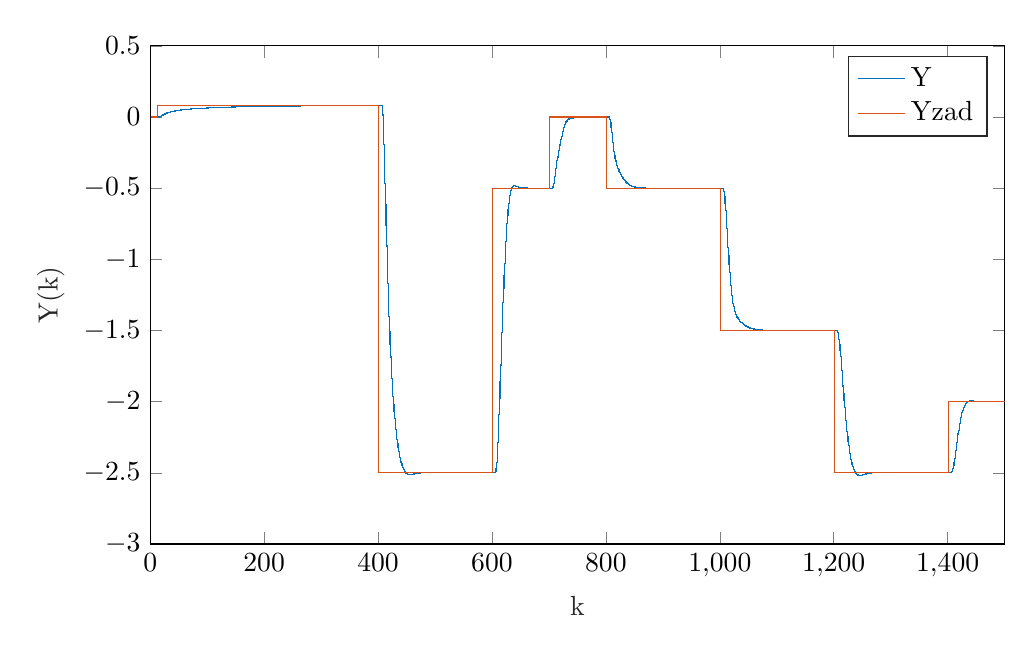
\begin{tikzpicture}

\begin{axis}[%
width=4.272in,
height=2.491in,
at={(0.717in,0.423in)},
scale only axis,
xmin=0,
xmax=1500,
xlabel style={font=\color{white!15!black}},
xlabel={k},
ymin=-3,
ymax=0.5,
ylabel style={font=\color{white!15!black}},
ylabel={Y(k)},
axis background/.style={fill=white},
legend style={legend cell align=left, align=left, draw=white!15!black}
]
\addplot[const plot, color=mycolor1] table[row sep=crcr] {%
1	0\\
2	0\\
3	0\\
4	0\\
5	0\\
6	0\\
7	0\\
8	0\\
9	0\\
10	0\\
11	0\\
12	0\\
13	0\\
14	0\\
15	0\\
16	0\\
17	0.00058843553592282\\
18	0.002233596388619\\
19	0.00474220844281684\\
20	0.00772355260990064\\
21	0.0108220920955545\\
22	0.0137993985108358\\
23	0.0165345147680059\\
24	0.0189906952958731\\
25	0.0211788856934875\\
26	0.0231305545692476\\
27	0.0248816664717093\\
28	0.026467631693033\\
29	0.0279233542123638\\
30	0.0292790626691571\\
31	0.0305564191645399\\
32	0.0317695048676013\\
33	0.0329271145584383\\
34	0.0340348212668022\\
35	0.0350963853953937\\
36	0.0361145891635708\\
37	0.0370917014208645\\
38	0.0380297300273955\\
39	0.0389305530206983\\
40	0.0397959833766321\\
41	0.0406277952355082\\
42	0.0414277286825868\\
43	0.0421974843401344\\
44	0.042938714820553\\
45	0.0436530168487208\\
46	0.0443419255667411\\
47	0.0450069111795587\\
48	0.0456493774970553\\
49	0.0462706617988136\\
50	0.0468720355418124\\
51	0.047454705583857\\
52	0.0480198157259568\\
53	0.0485684484622509\\
54	0.0491016268722708\\
55	0.04962031661169\\
56	0.0501254279668873\\
57	0.0506177101630945\\
58	0.0510960155540965\\
59	0.0515591268505437\\
60	0.0520066554767782\\
61	0.0524389084153513\\
62	0.0528565808010423\\
63	0.0532605227429185\\
64	0.0536516156624629\\
65	0.0540307174568761\\
66	0.0543986392934862\\
67	0.0547561359046759\\
68	0.0551039023482373\\
69	0.05544257450117\\
70	0.0557727318441523\\
71	0.0560949015085359\\
72	0.0564095628355855\\
73	0.0567171519598847\\
74	0.0570180661456812\\
75	0.057312667754839\\
76	0.057601287813818\\
77	0.057884229192572\\
78	0.0581617694277871\\
79	0.0584341632286968\\
80	0.0587016447030857\\
81	0.0589644293378635\\
82	0.0592227157645995\\
83	0.0594766873364753\\
84	0.0597265135395442\\
85	0.059972351258071\\
86	0.0602143459110481\\
87	0.0604526324747046\\
88	0.060687336403881\\
89	0.0609185744634895\\
90	0.0611464554798633\\
91	0.0613710810205884\\
92	0.0615925460103693\\
93	0.0618109392895804\\
94	0.0620263441213774\\
95	0.0622388373202954\\
96	0.0624484805566784\\
97	0.0626553266610378\\
98	0.0628594307457025\\
99	0.0630608498141013\\
100	0.0632596407925237\\
101	0.063455859169011\\
102	0.0636495583765785\\
103	0.0638407896187546\\
104	0.0640296018723241\\
105	0.0642160419569574\\
106	0.0644001546339039\\
107	0.0645819827190562\\
108	0.0647615672020437\\
109	0.0649389473655107\\
110	0.0651141609006494\\
111	0.0652872440166914\\
112	0.065458231543281\\
113	0.0656271570254397\\
114	0.0657940528112799\\
115	0.0659589501328465\\
116	0.0661218791805539\\
117	0.066282869171709\\
118	0.0664419484135918\\
119	0.0665991443615425\\
120	0.0667544836724651\\
121	0.0669079922541288\\
122	0.0670596953106137\\
123	0.0672096173842191\\
124	0.0673577823941241\\
125	0.0675042136720687\\
126	0.0676489339952961\\
127	0.0677919656169806\\
128	0.0679333302943454\\
129	0.0680730493146556\\
130	0.0682111435192597\\
131	0.0683476333258352\\
132	0.0684825387489831\\
133	0.0686158794193036\\
134	0.0687476746010733\\
135	0.0688779432086365\\
136	0.0690067038216124\\
137	0.0691339746990118\\
138	0.0692597737923502\\
139	0.0693841187578354\\
140	0.0695070269677048\\
141	0.0696285155207765\\
142	0.0697486012522786\\
143	0.0698673007430107\\
144	0.069984630327892\\
145	0.070100606103943\\
146	0.0702152439377446\\
147	0.0703285594724155\\
148	0.0704405681341456\\
149	0.0705512851383195\\
150	0.0706607254952615\\
151	0.0707689040156321\\
152	0.0708758353155013\\
153	0.0709815338211257\\
154	0.0710860137734496\\
155	0.0711892892323533\\
156	0.0712913740806665\\
157	0.0713922820279649\\
158	0.0714920266141668\\
159	0.0715906212129445\\
160	0.0716880790349643\\
161	0.0717844131309681\\
162	0.0718796363947079\\
163	0.0719737615657454\\
164	0.0720668012321249\\
165	0.0721587678329304\\
166	0.0722496736607339\\
167	0.0723395308639441\\
168	0.0724283514490618\\
169	0.0725161472828489\\
170	0.0726029303623798\\
171	0.072688713895758\\
172	0.0727735122783488\\
173	0.0728573386421239\\
174	0.0729402050043145\\
175	0.0730221226859945\\
176	0.0731031025944485\\
177	0.0731831553692109\\
178	0.073262291450267\\
179	0.0733405211147862\\
180	0.0734178544997295\\
181	0.0734943016163817\\
182	0.0735698723596362\\
183	0.0736445765138754\\
184	0.0737184237567425\\
185	0.0737914236616724\\
186	0.0738635856997195\\
187	0.073934919240997\\
188	0.0740054335559023\\
189	0.0740751378162252\\
190	0.0741440410961877\\
191	0.0742121523734433\\
192	0.0742794805300491\\
193	0.074346034353418\\
194	0.0744118225372558\\
195	0.0744768536824842\\
196	0.0745411362981523\\
197	0.0746046788023366\\
198	0.0746674895230311\\
199	0.0747295766990268\\
200	0.0747909484807826\\
201	0.0748516129312863\\
202	0.0749115780269078\\
203	0.0749708516582433\\
204	0.0750294416309513\\
205	0.0750873556665819\\
206	0.0751446014033967\\
207	0.0752011863971834\\
208	0.075257118122061\\
209	0.0753124039712802\\
210	0.0753670512580151\\
211	0.0754210672161495\\
212	0.0754744590010558\\
213	0.0755272336903678\\
214	0.0755793982847471\\
215	0.0756309597086435\\
216	0.0756819248110482\\
217	0.0757323003662425\\
218	0.0757820930745393\\
219	0.0758313095630189\\
220	0.075879956386259\\
221	0.075928040027059\\
222	0.0759755668971581\\
223	0.0760225433379484\\
224	0.076068975621181\\
225	0.0761148699496681\\
226	0.0761602324579777\\
227	0.0762050692131243\\
228	0.0762493862152528\\
229	0.0762931893983179\\
230	0.0763364846307566\\
231	0.0763792777161568\\
232	0.0764215743939192\\
233	0.0764633803399146\\
234	0.0765047011671347\\
235	0.0765455424263389\\
236	0.0765859096066945\\
237	0.0766258081364123\\
238	0.0766652433833761\\
239	0.0767042206557679\\
240	0.0767427452026868\\
241	0.076780822214763\\
242	0.0768184568247668\\
243	0.0768556541082121\\
244	0.0768924190839542\\
245	0.0769287567147832\\
246	0.0769646719080122\\
247	0.077000169516059\\
248	0.0770352543370248\\
249	0.0770699311152653\\
250	0.0771042045419594\\
251	0.0771380792556701\\
252	0.0771715598429026\\
253	0.0772046508386557\\
254	0.0772373567269694\\
255	0.0772696819414665\\
256	0.0773016308658903\\
257	0.0773332078346359\\
258	0.0773644171332784\\
259	0.0773952629990945\\
260	0.0774257496215802\\
261	0.0774558811429636\\
262	0.0774856616587126\\
263	0.0775150952180376\\
264	0.0775441858243903\\
265	0.0775729374359567\\
266	0.0776013539661462\\
267	0.0776294392840756\\
268	0.0776571972150486\\
269	0.0776846315410306\\
270	0.077711746001119\\
271	0.0777385442920089\\
272	0.077765030068454\\
273	0.0777912069437237\\
274	0.0778170784900547\\
275	0.0778426482390992\\
276	0.0778679196823678\\
277	0.0778928962716688\\
278	0.0779175814195425\\
279	0.0779419784996915\\
280	0.0779660908474065\\
281	0.0779899217599883\\
282	0.0780134744971649\\
283	0.0780367522815051\\
284	0.0780597582988274\\
285	0.0780824956986049\\
286	0.0781049675943662\\
287	0.0781271770640922\\
288	0.0781491271506089\\
289	0.0781708208619761\\
290	0.078192261171872\\
291	0.0782134510199743\\
292	0.0782343933123369\\
293	0.0782550909217629\\
294	0.0782755466881739\\
295	0.0782957634189753\\
296	0.078315743889418\\
297	0.0783354908429558\\
298	0.0783550069916002\\
299	0.07837429501627\\
300	0.0783933575671389\\
301	0.0784121972639779\\
302	0.0784308166964952\\
303	0.0784492184246722\\
304	0.0784674049790959\\
305	0.0784853788612876\\
306	0.0785031425440289\\
307	0.078520698471683\\
308	0.078538049060514\\
309	0.078555196699002\\
310	0.0785721437481546\\
311	0.0785888925418159\\
312	0.0786054453869719\\
313	0.078621804564052\\
314	0.0786379723272285\\
315	0.0786539509047117\\
316	0.0786697424990427\\
317	0.0786853492873825\\
318	0.0787007734217983\\
319	0.078716017029547\\
320	0.0787310822133546\\
321	0.0787459710516939\\
322	0.0787606855990583\\
323	0.078775227886233\\
324	0.0787895999205634\\
325	0.07880380368622\\
326	0.0788178411444612\\
327	0.0788317142338925\\
328	0.0788454248707236\\
329	0.0788589749490224\\
330	0.0788723663409657\\
331	0.0788856008970884\\
332	0.0788986804465286\\
333	0.0789116067972709\\
334	0.078924381736387\\
335	0.0789370070302732\\
336	0.0789494844248856\\
337	0.0789618156459731\\
338	0.0789740023993067\\
339	0.0789860463709077\\
340	0.0789979492272725\\
341	0.0790097126155951\\
342	0.0790213381639869\\
343	0.0790328274816949\\
344	0.0790441821593167\\
345	0.0790554037690133\\
346	0.0790664938647197\\
347	0.0790774539823533\\
348	0.0790882856400194\\
349	0.0790989903382151\\
350	0.0791095695600307\\
351	0.0791200247713486\\
352	0.0791303574210403\\
353	0.0791405689411612\\
354	0.0791506607471431\\
355	0.0791606342379846\\
356	0.0791704907964396\\
357	0.079180231789203\\
358	0.0791898585670954\\
359	0.0791993724652447\\
360	0.0792087748032665\\
361	0.0792180668854419\\
362	0.0792272500008936\\
363	0.0792363254237599\\
364	0.0792452944133669\\
365	0.0792541582143985\\
366	0.079262918057065\\
367	0.0792715751572693\\
368	0.0792801307167713\\
369	0.0792885859233508\\
370	0.079296941950968\\
371	0.0793051999599232\\
372	0.0793133610970133\\
373	0.0793214264956876\\
374	0.0793293972762018\\
375	0.0793372745457695\\
376	0.0793450593987126\\
377	0.0793527529166103\\
378	0.0793603561684454\\
379	0.0793678702107501\\
380	0.079375296087749\\
381	0.0793826348315019\\
382	0.0793898874620433\\
383	0.0793970549875219\\
384	0.0794041384043373\\
385	0.0794111386972761\\
386	0.0794180568396457\\
387	0.079424893793407\\
388	0.0794316505093056\\
389	0.0794383279270015\\
390	0.0794449269751968\\
391	0.0794514485717628\\
392	0.0794578936238653\\
393	0.0794642630280882\\
394	0.0794705576705557\\
395	0.079476778427054\\
396	0.0794829261631504\\
397	0.0794890017343118\\
398	0.0794950059860214\\
399	0.0795009397538949\\
400	0.079506803863794\\
401	0.0795125991319401\\
402	0.0795183263650253\\
403	0.0795239863603236\\
404	0.0795295799057994\\
405	0.0795351077802158\\
406	0.0830769280807187\\
407	0.0699222322373291\\
408	0.0135779084748505\\
409	-0.0761726075628852\\
410	-0.190961586886551\\
411	-0.3236260787352\\
412	-0.467261502196576\\
413	-0.615580526490898\\
414	-0.763280416254029\\
415	-0.906639849662523\\
416	-1.04334724800793\\
417	-1.17206336719653\\
418	-1.29212062683365\\
419	-1.40331785599191\\
420	-1.50577761946212\\
421	-1.59984290451115\\
422	-1.68599917406959\\
423	-1.76481406169677\\
424	-1.83689056862036\\
425	-1.90283146775534\\
426	-1.96320540779883\\
427	-2.018528459508\\
428	-2.06925780131407\\
429	-2.11579200455448\\
430	-2.15847539938443\\
431	-2.19760462301857\\
432	-2.23343606079624\\
433	-2.26619338232285\\
434	-2.2960745883483\\
435	-2.32325818849837\\
436	-2.34790832400038\\
437	-2.37017879278596\\
438	-2.3902160333414\\
439	-2.40816118651594\\
440	-2.42415138924612\\
441	-2.43832046553625\\
442	-2.45079917295868\\
443	-2.46171514391453\\
444	-2.47119263599529\\
445	-2.47935217966545\\
446	-2.48631019448797\\
447	-2.49217861254606\\
448	-2.49706453083116\\
449	-2.50106990562118\\
450	-2.50429129588969\\
451	-2.5068196592837\\
452	-2.50874020214709\\
453	-2.51013228376026\\
454	-2.51106937413217\\
455	-2.51161906403465\\
456	-2.5118431253362\\
457	-2.51179761901653\\
458	-2.51153304753312\\
459	-2.51109454750873\\
460	-2.51052211806812\\
461	-2.50985087962545\\
462	-2.50911135755262\\
463	-2.50832978496845\\
464	-2.50752841888494\\
465	-2.50672586412054\\
466	-2.50593739971191\\
467	-2.50517530301012\\
468	-2.50444916719354\\
469	-2.50376620852968\\
470	-2.503131560339\\
471	-2.50254855122917\\
472	-2.50201896575676\\
473	-2.50154328622086\\
474	-2.50112091478917\\
475	-2.50075037559637\\
476	-2.50042949683559\\
477	-2.50015557318564\\
478	-2.4999255091835\\
479	-2.49973594436543\\
480	-2.49958336116618\\
481	-2.49946417668865\\
482	-2.49937481954055\\
483	-2.49931179298521\\
484	-2.49927172567508\\
485	-2.49925141123325\\
486	-2.49924783792388\\
487	-2.49925820961173\\
488	-2.49927995915604\\
489	-2.49931075531901\\
490	-2.49934850419658\\
491	-2.49939134610124\\
492	-2.49943764874597\\
493	-2.49948599749674\\
494	-2.49953518337964\\
495	-2.49958418944964\\
496	-2.49963217605157\\
497	-2.49967846543129\\
498	-2.49972252608735\\
499	-2.49976395718976\\
500	-2.49980247333492\\
501	-2.49983788985266\\
502	-2.49987010883434\\
503	-2.49989910600827\\
504	-2.49992491855204\\
505	-2.49994763389884\\
506	-2.49996737956716\\
507	-2.49998431401995\\
508	-2.49999861853972\\
509	-2.50001049009025\\
510	-2.50002013512302\\
511	-2.50002776427665\\
512	-2.50003358791083\\
513	-2.50003781241095\\
514	-2.50004063719735\\
515	-2.50004225237143\\
516	-2.5000428369314\\
517	-2.50004255749178\\
518	-2.50004156744295\\
519	-2.50004000649034\\
520	-2.50003800051627\\
521	-2.50003566171158\\
522	-2.50003308892845\\
523	-2.50003036821015\\
524	-2.50002757345788\\
525	-2.50002476719942\\
526	-2.50002200142834\\
527	-2.50001931848672\\
528	-2.50001675196829\\
529	-2.50001432762222\\
530	-2.50001206424158\\
531	-2.50000997452307\\
532	-2.50000806588777\\
533	-2.50000634125493\\
534	-2.5000047997631\\
535	-2.50000343743477\\
536	-2.50000224778242\\
537	-2.50000122235516\\
538	-2.50000035122659\\
539	-2.49999962342502\\
540	-2.49999902730858\\
541	-2.49999855088778\\
542	-2.49999818209884\\
543	-2.49999790903149\\
544	-2.49999772011485\\
545	-2.49999760426535\\
546	-2.49999755100057\\
547	-2.49999755052285\\
548	-2.49999759377626\\
549	-2.49999767248063\\
550	-2.49999777914593\\
551	-2.49999790706999\\
552	-2.49999805032273\\
553	-2.49999820371919\\
554	-2.499998362784\\
555	-2.49999852370928\\
556	-2.4999986833079\\
557	-2.49999883896364\\
558	-2.49999898857979\\
559	-2.49999913052732\\
560	-2.4999992635936\\
561	-2.49999938693247\\
562	-2.49999950001643\\
563	-2.4999996025913\\
564	-2.49999969463381\\
565	-2.49999977631239\\
566	-2.49999984795122\\
567	-2.49999990999773\\
568	-2.49999996299343\\
569	-2.50000000754814\\
570	-2.5000000443174\\
571	-2.50000007398288\\
572	-2.50000009723582\\
573	-2.500000114763\\
574	-2.50000012723532\\
575	-2.50000013529854\\
576	-2.50000013956611\\
577	-2.50000014061377\\
578	-2.50000013897578\\
579	-2.5000001351425\\
580	-2.50000012955922\\
581	-2.50000012262595\\
582	-2.50000011469805\\
583	-2.5000001060876\\
584	-2.50000009706525\\
585	-2.5000000878625\\
586	-2.50000007867434\\
587	-2.50000006966198\\
588	-2.50000006095585\\
589	-2.50000005265849\\
590	-2.50000004484758\\
591	-2.50000003757877\\
592	-2.5000000308885\\
593	-2.50000002479665\\
594	-2.50000001930902\\
595	-2.50000001441963\\
596	-2.50000001011289\\
597	-2.5000000063655\\
598	-2.50000000314817\\
599	-2.50000000042722\\
600	-2.4999999981659\\
601	-2.49999999632558\\
602	-2.49999999486676\\
603	-2.49999999374992\\
604	-2.49999999293624\\
605	-2.49999999238816\\
606	-2.49210601614885\\
607	-2.46912906003041\\
608	-2.42758377253649\\
609	-2.36680010662485\\
610	-2.28815418111409\\
611	-2.19439874357448\\
612	-2.08909350105406\\
613	-1.97613793507788\\
614	-1.85940503143637\\
615	-1.74218397045676\\
616	-1.62683725778706\\
617	-1.51491819718118\\
618	-1.40738430039358\\
619	-1.30479434075913\\
620	-1.20747549410567\\
621	-1.11565079126183\\
622	-1.02952204522942\\
623	-0.949309122640208\\
624	-0.875252210216554\\
625	-0.807739928366552\\
626	-0.74718386394065\\
627	-0.693857824034011\\
628	-0.647816540133827\\
629	-0.608880749681589\\
630	-0.576663378878263\\
631	-0.55061656563256\\
632	-0.530085445821116\\
633	-0.514359734628504\\
634	-0.502718062337814\\
635	-0.494462876040364\\
636	-0.488945616261756\\
637	-0.485582995206557\\
638	-0.483865745740172\\
639	-0.483361374608849\\
640	-0.483712398920188\\
641	-0.484631385728228\\
642	-0.485893920720714\\
643	-0.48733043575519\\
644	-0.488817637788158\\
645	-0.490270107189813\\
646	-0.491632464885646\\
647	-0.492872392381734\\
648	-0.493974642368958\\
649	-0.494936072805914\\
650	-0.49576166770922\\
651	-0.496461458004985\\
652	-0.497048224927486\\
653	-0.497535855110632\\
654	-0.497938217308888\\
655	-0.4982684413202\\
656	-0.498538495967853\\
657	-0.498758981427021\\
658	-0.498939069217159\\
659	-0.499086539266291\\
660	-0.499207876862452\\
661	-0.499308402919958\\
662	-0.499392419055062\\
663	-0.49946335491983\\
664	-0.49952390955803\\
665	-0.499576181649363\\
666	-0.49962178574557\\
667	-0.499661953191774\\
668	-0.499697617588588\\
669	-0.499729485471141\\
670	-0.499758093424199\\
671	-0.499783853177136\\
672	-0.499807086373914\\
673	-0.499828050729507\\
674	-0.499846959200091\\
675	-0.499863993642105\\
676	-0.499879314243816\\
677	-0.499893065806436\\
678	-0.499905381748736\\
679	-0.499916386522268\\
680	-0.499926196961187\\
681	-0.499934922954318\\
682	-0.499942667717304\\
683	-0.499949527857141\\
684	-0.499955593356706\\
685	-0.499960947559273\\
686	-0.499965667198922\\
687	-0.499969822498995\\
688	-0.499973477344794\\
689	-0.499976689526474\\
690	-0.499979511041962\\
691	-0.499981988446665\\
692	-0.499984163235707\\
693	-0.499986072244821\\
694	-0.499987748057389\\
695	-0.499989219406946\\
696	-0.499990511566539\\
697	-0.499991646718456\\
698	-0.499992644299791\\
699	-0.499993521321061\\
700	-0.499994292656544\\
701	-0.499994971306221\\
702	-0.499995568630027\\
703	-0.499996094555836\\
704	-0.499996557762959\\
705	-0.499996965843204\\
706	-0.49625927394527\\
707	-0.486076486598276\\
708	-0.46901571095024\\
709	-0.446088990299458\\
710	-0.419055511404253\\
711	-0.389878833727871\\
712	-0.36035773316958\\
713	-0.331921135301149\\
714	-0.305397846632133\\
715	-0.28094234330471\\
716	-0.258278381657738\\
717	-0.236962165984335\\
718	-0.216559997104507\\
719	-0.196747928045934\\
720	-0.177351583577472\\
721	-0.158346336499917\\
722	-0.139834018497598\\
723	-0.122006961995048\\
724	-0.10510613879596\\
725	-0.0893784624485982\\
726	-0.0750383405306965\\
727	-0.0622537771460652\\
728	-0.0511596393900556\\
729	-0.0418066428649104\\
730	-0.0341305719590848\\
731	-0.0279739230582431\\
732	-0.0231256849991289\\
733	-0.0193584603140994\\
734	-0.0164545591443314\\
735	-0.0142207642758465\\
736	-0.0124945743106523\\
737	-0.0111449788828351\\
738	-0.0100701119685139\\
739	-0.00919334783412446\\
740	-0.00845882611093314\\
741	-0.00782701925738696\\
742	-0.00727071352593595\\
743	-0.00677160330048002\\
744	-0.00631756992164324\\
745	-0.00590062242090725\\
746	-0.00551541793748375\\
747	-0.00515825108659443\\
748	-0.00482639756320049\\
749	-0.00451770919101579\\
750	-0.00423037726499012\\
751	-0.00396280217962534\\
752	-0.00371352622870762\\
753	-0.00348120146005805\\
754	-0.00326457536939239\\
755	-0.00306248458117868\\
756	-0.0028738513185069\\
757	-0.00269768021894962\\
758	-0.00253305457201484\\
759	-0.00237913181814282\\
760	-0.00223513848126353\\
761	-0.00210036480788004\\
762	-0.0019741593743563\\
763	-0.00185592386727387\\
764	-0.00174510817462749\\
765	-0.00164120586518163\\
766	-0.00154375008609499\\
767	-0.00145230987593452\\
768	-0.0013664868697063\\
769	-0.00128591236172906\\
770	-0.00121024468818183\\
771	-0.00113916689148025\\
772	-0.00107238463136856\\
773	-0.00100962431143368\\
774	-0.000950631393820454\\
775	-0.00089516887878858\\
776	-0.000843015929184809\\
777	-0.000793966622844926\\
778	-0.000747828818406087\\
779	-0.000704423122057956\\
780	-0.000663581944457509\\
781	-0.000625148638441877\\
782	-0.000588976709352143\\
783	-0.000554929090774388\\
784	-0.000522877479348849\\
785	-0.000492701723022113\\
786	-0.000464289257742683\\
787	-0.000437534588143935\\
788	-0.00041233880823364\\
789	-0.000388609158526252\\
790	-0.000366258616421406\\
791	-0.000345205516956382\\
792	-0.000325373201347303\\
793	-0.000306689690988312\\
794	-0.00028908738480407\\
795	-0.000272502778052012\\
796	-0.000256876200850029\\
797	-0.000242151574865217\\
798	-0.000228276186742313\\
799	-0.000215200476978454\\
800	-0.000202877843065747\\
801	-0.000191264455826203\\
802	-0.000180319087956402\\
803	-0.000170002953882814\\
804	-0.000160279560104147\\
805	-0.000151114565265236\\
806	-0.00418896493305138\\
807	-0.0172882661457858\\
808	-0.0404072159566166\\
809	-0.0715211912373293\\
810	-0.107353874652058\\
811	-0.14464527709013\\
812	-0.180713089996021\\
813	-0.213790656723191\\
814	-0.243098945238822\\
815	-0.268534439601354\\
816	-0.290358424588273\\
817	-0.309006299720353\\
818	-0.324975510918946\\
819	-0.338760527873641\\
820	-0.350815183124283\\
821	-0.361531936003073\\
822	-0.371232634613881\\
823	-0.380167552506093\\
824	-0.388520317804387\\
825	-0.396416680478687\\
826	-0.403932636531107\\
827	-0.411107723308431\\
828	-0.417957776228766\\
829	-0.424484659704213\\
830	-0.430683334453731\\
831	-0.436546689932375\\
832	-0.442068616623767\\
833	-0.447245755387074\\
834	-0.452078291312671\\
835	-0.456570095072948\\
836	-0.460728455669709\\
837	-0.464563591520925\\
838	-0.468088074418742\\
839	-0.471316255192868\\
840	-0.474263741194392\\
841	-0.476946946275174\\
842	-0.479382715149005\\
843	-0.481588014521268\\
844	-0.48357968041831\\
845	-0.485374211927356\\
846	-0.486987605979191\\
847	-0.488435223264602\\
848	-0.489731682916982\\
849	-0.490890785588191\\
850	-0.491925463308617\\
851	-0.492847753541089\\
852	-0.493668794138466\\
853	-0.494398835569783\\
854	-0.495047266762522\\
855	-0.495622651131457\\
856	-0.496132769741159\\
857	-0.496584669006991\\
858	-0.496984710818823\\
859	-0.497338623429413\\
860	-0.497651551858854\\
861	-0.497928106913116\\
862	-0.498172412193426\\
863	-0.498388148687602\\
864	-0.498578596693677\\
865	-0.498746674941834\\
866	-0.498894976862632\\
867	-0.499025804015212\\
868	-0.499141196732946\\
869	-0.499242962077034\\
870	-0.499332699215646\\
871	-0.499411822367479\\
872	-0.499481581463921\\
873	-0.499543080693632\\
874	-0.499597295097488\\
875	-0.499645085381328\\
876	-0.499687211109543\\
877	-0.499724342435278\\
878	-0.499757070513808\\
879	-0.499785916735173\\
880	-0.499811340901254\\
881	-0.499833748461456\\
882	-0.4998534969105\\
883	-0.499870901441735\\
884	-0.499886239939868\\
885	-0.499899757388361\\
886	-0.499911669758684\\
887	-0.499922167441382\\
888	-0.499931418272287\\
889	-0.499939570201255\\
890	-0.499946753645435\\
891	-0.499953083564261\\
892	-0.499958661289025\\
893	-0.499963576136073\\
894	-0.499967906829222\\
895	-0.499971722753977\\
896	-0.499975085063451\\
897	-0.499978047653519\\
898	-0.499980658022674\\
899	-0.499982958030201\\
900	-0.499984984564674\\
901	-0.499986770133374\\
902	-0.49998834338196\\
903	-0.499989729552628\\
904	-0.49999095088802\\
905	-0.499992026987298\\
906	-0.499992975120021\\
907	-0.499993810502824\\
908	-0.499994546543286\\
909	-0.499995195054879\\
910	-0.499995766446408\\
911	-0.499996269888959\\
912	-0.499996713463042\\
913	-0.49999710428824\\
914	-0.499997448637465\\
915	-0.499997752037637\\
916	-0.499998019358394\\
917	-0.499998254890257\\
918	-0.499998462413504\\
919	-0.499998645258852\\
920	-0.49999880636092\\
921	-0.499998948305341\\
922	-0.499999073370267\\
923	-0.499999183562933\\
924	-0.49999928065188\\
925	-0.49999936619534\\
926	-0.499999441566245\\
927	-0.499999507974268\\
928	-0.499999566485233\\
929	-0.499999618038221\\
930	-0.499999663460646\\
931	-0.49999970348153\\
932	-0.499999738743203\\
933	-0.499999769811617\\
934	-0.499999797185419\\
935	-0.499999821303964\\
936	-0.499999842554358\\
937	-0.499999861277677\\
938	-0.499999877774436\\
939	-0.499999892309413\\
940	-0.499999905115901\\
941	-0.499999916399451\\
942	-0.499999926341168\\
943	-0.499999935100622\\
944	-0.499999942818408\\
945	-0.499999949618399\\
946	-0.49999995560974\\
947	-0.499999960888594\\
948	-0.499999965539691\\
949	-0.499999969637682\\
950	-0.499999973248344\\
951	-0.499999976429628\\
952	-0.499999979232596\\
953	-0.499999981702238\\
954	-0.499999983878192\\
955	-0.499999985795383\\
956	-0.499999987484583\\
957	-0.499999988972906\\
958	-0.499999990284238\\
959	-0.499999991439628\\
960	-0.49999999245762\\
961	-0.499999993354553\\
962	-0.499999994144824\\
963	-0.499999994841116\\
964	-0.499999995454606\\
965	-0.49999999599514\\
966	-0.499999996471395\\
967	-0.499999996891014\\
968	-0.499999997260732\\
969	-0.499999997586483\\
970	-0.499999997873497\\
971	-0.499999998126379\\
972	-0.499999998349188\\
973	-0.499999998545502\\
974	-0.499999998718469\\
975	-0.499999998870868\\
976	-0.499999999005143\\
977	-0.499999999123451\\
978	-0.499999999227689\\
979	-0.499999999319532\\
980	-0.499999999400452\\
981	-0.49999999947175\\
982	-0.499999999534569\\
983	-0.499999999589918\\
984	-0.499999999638684\\
985	-0.499999999681652\\
986	-0.499999999719509\\
987	-0.499999999752865\\
988	-0.499999999782254\\
989	-0.499999999808149\\
990	-0.499999999830963\\
991	-0.499999999851065\\
992	-0.499999999868776\\
993	-0.499999999884381\\
994	-0.499999999898131\\
995	-0.499999999910245\\
996	-0.499999999920918\\
997	-0.499999999930323\\
998	-0.499999999938609\\
999	-0.499999999945909\\
1000	-0.499999999952342\\
1001	-0.499999999958009\\
1002	-0.499999999963003\\
1003	-0.499999999967403\\
1004	-0.499999999971279\\
1005	-0.499999999974695\\
1006	-0.507100659820895\\
1007	-0.526407591821294\\
1008	-0.559194379138766\\
1009	-0.60414802971977\\
1010	-0.658624389755372\\
1011	-0.719602782809143\\
1012	-0.78420002234564\\
1013	-0.849908617644206\\
1014	-0.914677632545712\\
1015	-0.976913271122816\\
1016	-1.03544361781865\\
1017	-1.08947029048353\\
1018	-1.13851700222958\\
1019	-1.18237853763366\\
1020	-1.22107111771552\\
1021	-1.25480603143375\\
1022	-1.28393633815249\\
1023	-1.30889960719954\\
1024	-1.3301733460328\\
1025	-1.34824211426292\\
1026	-1.36357080324715\\
1027	-1.3765884789912\\
1028	-1.38768011395972\\
1029	-1.39718323461391\\
1030	-1.4053879235198\\
1031	-1.4125390405183\\
1032	-1.41883983125272\\
1033	-1.42445630876954\\
1034	-1.42952195690214\\
1035	-1.43414243186317\\
1036	-1.43840004074747\\
1037	-1.44235785696041\\
1038	-1.44606339551446\\
1039	-1.44955181794695\\
1040	-1.45284866969251\\
1041	-1.45597217460439\\
1042	-1.4589351244263\\
1043	-1.46174640762391\\
1044	-1.46441222401473\\
1045	-1.4669370306301\\
1046	-1.46932426425849\\
1047	-1.47157687745932\\
1048	-1.47369772034962\\
1049	-1.47568979728525\\
1050	-1.47755642413234\\
1051	-1.4793013084832\\
1052	-1.48092857195631\\
1053	-1.48244273068885\\
1054	-1.48384864732945\\
1055	-1.48515146529903\\
1056	-1.4863565338244\\
1057	-1.48746933026715\\
1058	-1.48849538456547\\
1059	-1.48944020916781\\
1060	-1.49030923665028\\
1061	-1.49110776625331\\
1062	-1.49184091982629\\
1063	-1.49251360710536\\
1064	-1.49313049984509\\
1065	-1.49369601405261\\
1066	-1.49421429940689\\
1067	-1.4946892348689\\
1068	-1.49512442947784\\
1069	-1.49552322736491\\
1070	-1.49588871608403\\
1071	-1.4962237374463\\
1072	-1.49653090014268\\
1073	-1.49681259353938\\
1074	-1.49707100212916\\
1075	-1.49730812021424\\
1076	-1.49752576648143\\
1077	-1.49772559820622\\
1078	-1.49790912488885\\
1079	-1.49807772118244\\
1080	-1.49823263902116\\
1081	-1.49837501889601\\
1082	-1.49850590025739\\
1083	-1.49862623104897\\
1084	-1.49873687639629\\
1085	-1.49883862648736\\
1086	-1.49893220369254\\
1087	-1.49901826897677\\
1088	-1.49909742766062\\
1089	-1.49917023458734\\
1090	-1.49923719875259\\
1091	-1.499298787451\\
1092	-1.49935542999093\\
1093	-1.49940752102496\\
1094	-1.49945542353977\\
1095	-1.49949947154481\\
1096	-1.49953997249519\\
1097	-1.49957720948016\\
1098	-1.49961144320483\\
1099	-1.49964291378951\\
1100	-1.49967184240755\\
1101	-1.49969843278022\\
1102	-1.49972287254431\\
1103	-1.49974533450604\\
1104	-1.49976597779325\\
1105	-1.49978494891568\\
1106	-1.49980238274243\\
1107	-1.49981840340395\\
1108	-1.49983312512518\\
1109	-1.49984665299576\\
1110	-1.49985908368225\\
1111	-1.4998705060869\\
1112	-1.49988100195711\\
1113	-1.49989064644909\\
1114	-1.4998995086491\\
1115	-1.49990765205533\\
1116	-1.49991513502311\\
1117	-1.49992201117613\\
1118	-1.49992832978603\\
1119	-1.49993413612255\\
1120	-1.49993947177644\\
1121	-1.49994437495707\\
1122	-1.49994888076641\\
1123	-1.49995302145143\\
1124	-1.49995682663622\\
1125	-1.49996032353551\\
1126	-1.49996353715106\\
1127	-1.49996649045201\\
1128	-1.49996920454075\\
1129	-1.49997169880515\\
1130	-1.49997399105845\\
1131	-1.49997609766767\\
1132	-1.49997803367155\\
1133	-1.49997981288876\\
1134	-1.49998144801732\\
1135	-1.49998295072578\\
1136	-1.49998433173702\\
1137	-1.4999856009051\\
1138	-1.49998676728586\\
1139	-1.49998783920174\\
1140	-1.49998882430131\\
1141	-1.49998972961387\\
1142	-1.49999056159974\\
1143	-1.49999132619625\\
1144	-1.4999920288602\\
1145	-1.49999267460672\\
1146	-1.499993268045\\
1147	-1.49999381341118\\
1148	-1.49999431459852\\
1149	-1.49999477518513\\
1150	-1.49999519845945\\
1151	-1.49999558744373\\
1152	-1.49999594491551\\
1153	-1.49999627342745\\
1154	-1.49999657532549\\
1155	-1.49999685276562\\
1156	-1.4999971077292\\
1157	-1.49999734203713\\
1158	-1.49999755736281\\
1159	-1.4999977552441\\
1160	-1.49999793709428\\
1161	-1.49999810421213\\
1162	-1.49999825779123\\
1163	-1.49999839892844\\
1164	-1.49999852863178\\
1165	-1.49999864782757\\
1166	-1.4999987573671\\
1167	-1.49999885803268\\
1168	-1.49999895054324\\
1169	-1.49999903555945\\
1170	-1.49999911368846\\
1171	-1.49999918548822\\
1172	-1.49999925147149\\
1173	-1.49999931210948\\
1174	-1.49999936783521\\
1175	-1.49999941904662\\
1176	-1.49999946610943\\
1177	-1.49999950935972\\
1178	-1.49999954910633\\
1179	-1.49999958563311\\
1180	-1.49999961920087\\
1181	-1.49999965004934\\
1182	-1.49999967839879\\
1183	-1.49999970445167\\
1184	-1.49999972839403\\
1185	-1.49999975039683\\
1186	-1.49999977061719\\
1187	-1.4999997891995\\
1188	-1.49999980627647\\
1189	-1.49999982197004\\
1190	-1.49999983639227\\
1191	-1.49999984964616\\
1192	-1.49999986182635\\
1193	-1.49999987301982\\
1194	-1.49999988330651\\
1195	-1.49999989275988\\
1196	-1.49999990144742\\
1197	-1.49999990943118\\
1198	-1.49999991676818\\
1199	-1.49999992351081\\
1200	-1.49999992970721\\
1201	-1.49999993540164\\
1202	-1.49999994063477\\
1203	-1.49999994544395\\
1204	-1.49999994986355\\
1205	-1.49999995392511\\
1206	-1.50381165496174\\
1207	-1.51458286701878\\
1208	-1.53358816874485\\
1209	-1.56085470517141\\
1210	-1.59563130572134\\
1211	-1.63673220400486\\
1212	-1.68278105024341\\
1213	-1.73237670806074\\
1214	-1.78419928447247\\
1215	-1.83707170906443\\
1216	-1.88998927351068\\
1217	-1.94212698437122\\
1218	-1.99283239011396\\
1219	-2.04160969700784\\
1220	-2.088099455466\\
1221	-2.13205684554622\\
1222	-2.17333058689791\\
1223	-2.21184371553814\\
1224	-2.24757687919772\\
1225	-2.28055437647734\\
1226	-2.31082967714593\\
1227	-2.33847619140596\\
1228	-2.36358204748015\\
1229	-2.38624684299286\\
1230	-2.4065795270159\\
1231	-2.42469684663781\\
1232	-2.44072200707541\\
1233	-2.45478335401487\\
1234	-2.46701299752907\\
1235	-2.47754536792441\\
1236	-2.48651573439278\\
1237	-2.49405873571814\\
1238	-2.500306975647\\
1239	-2.50538972964775\\
1240	-2.50943179906246\\
1241	-2.51255253625336\\
1242	-2.51486505234706\\
1243	-2.51647560880551\\
1244	-2.51748318587266\\
1245	-2.51797921507487\\
1246	-2.5180474620245\\
1247	-2.51776403912691\\
1248	-2.5171975269906\\
1249	-2.51640918502673\\
1250	-2.51545323368281\\
1251	-2.51437719287188\\
1252	-2.51322226316915\\
1253	-2.51202373812841\\
1254	-2.51081143759258\\
1255	-2.50961015316\\
1256	-2.50844009806962\\
1257	-2.50731735473611\\
1258	-2.50625431404692\\
1259	-2.50526010136095\\
1260	-2.50434098494383\\
1261	-2.50350076334655\\
1262	-2.50274112898099\\
1263	-2.50206200586229\\
1264	-2.50146186016277\\
1265	-2.50093798284572\\
1266	-2.50048674420705\\
1267	-2.50010382064866\\
1268	-2.49978439443071\\
1269	-2.49952332750028\\
1270	-2.49931531076994\\
1271	-2.49915499042713\\
1272	-2.49903707299833\\
1273	-2.49895641097901\\
1274	-2.49890807087733\\
1275	-2.49888738551651\\
1276	-2.49888999240237\\
1277	-2.49891185989864\\
1278	-2.49894930286666\\
1279	-2.49899898932611\\
1280	-2.49905793958197\\
1281	-2.49912351914557\\
1282	-2.49919342665688\\
1283	-2.49926567789426\\
1284	-2.49933858683842\\
1285	-2.49941074464218\\
1286	-2.49948099724693\\
1287	-2.49954842228215\\
1288	-2.49961230578699\\
1289	-2.49967211920264\\
1290	-2.49972749700152\\
1291	-2.49977821524477\\
1292	-2.4998241712922\\
1293	-2.49986536482989\\
1294	-2.49990188032798\\
1295	-2.49993387099666\\
1296	-2.49996154426937\\
1297	-2.49998514881027\\
1298	-2.50000496301596\\
1299	-2.50002128496014\\
1300	-2.50003442371273\\
1301	-2.5000446919524\\
1302	-2.50005239978214\\
1303	-2.50005784965166\\
1304	-2.50006133228709\\
1305	-2.50006312352778\\
1306	-2.50006348197081\\
1307	-2.50006264732662\\
1308	-2.50006083939299\\
1309	-2.50005825755967\\
1310	-2.50005508076131\\
1311	-2.5000514678027\\
1312	-2.50004755798655\\
1313	-2.5000434719809\\
1314	-2.50003931286936\\
1315	-2.50003516733432\\
1316	-2.50003110692907\\
1317	-2.50002718940106\\
1318	-2.50002346003383\\
1319	-2.50001995298056\\
1320	-2.500016692567\\
1321	-2.50001369454565\\
1322	-2.50001096728743\\
1323	-2.50000851290013\\
1324	-2.50000632826649\\
1325	-2.50000440599705\\
1326	-2.50000273529554\\
1327	-2.50000130273633\\
1328	-2.50000009295526\\
1329	-2.49999908925635\\
1330	-2.49999827413804\\
1331	-2.49999762974347\\
1332	-2.49999713823973\\
1333	-2.49999678213153\\
1334	-2.49999654451501\\
1335	-2.49999640927745\\
1336	-2.49999636124854\\
1337	-2.49999638630892\\
1338	-2.49999647146129\\
1339	-2.49999660486936\\
1340	-2.49999677586947\\
1341	-2.49999697495915\\
1342	-2.49999719376716\\
1343	-2.49999742500836\\
1344	-2.49999766242705\\
1345	-2.49999790073165\\
1346	-2.49999813552348\\
1347	-2.49999836322176\\
1348	-2.49999858098704\\
1349	-2.49999878664445\\
1350	-2.49999897860832\\
1351	-2.49999915580934\\
1352	-2.49999931762485\\
1353	-2.4999994638133\\
1354	-2.49999959445309\\
1355	-2.49999970988625\\
1356	-2.49999981066702\\
1357	-2.49999989751562\\
1358	-2.49999997127682\\
1359	-2.50000003288357\\
1360	-2.50000008332519\\
1361	-2.50000012362011\\
1362	-2.50000015479264\\
1363	-2.5000001778538\\
1364	-2.50000019378551\\
1365	-2.50000020352816\\
1366	-2.5000002079709\\
1367	-2.50000020794467\\
1368	-2.50000020421735\\
1369	-2.50000019749092\\
1370	-2.50000018840024\\
1371	-2.5000001775133\\
1372	-2.50000016533257\\
1373	-2.50000015229728\\
1374	-2.50000013878645\\
1375	-2.50000012512252\\
1376	-2.50000011157527\\
1377	-2.50000009836607\\
1378	-2.50000008567227\\
1379	-2.50000007363156\\
1380	-2.50000006234635\\
1381	-2.50000005188803\\
1382	-2.50000004230097\\
1383	-2.50000003360638\\
1384	-2.50000002580597\\
1385	-2.50000001888518\\
1386	-2.50000001281629\\
1387	-2.50000000756116\\
1388	-2.50000000307371\\
1389	-2.49999999930206\\
1390	-2.49999999619052\\
1391	-2.49999999368118\\
1392	-2.49999999171535\\
1393	-2.49999999023472\\
1394	-2.49999998918237\\
1395	-2.49999998850349\\
1396	-2.49999998814606\\
1397	-2.49999998806125\\
1398	-2.49999998820375\\
1399	-2.49999998853199\\
1400	-2.49999998900823\\
1401	-2.49999998959856\\
1402	-2.49999999027287\\
1403	-2.49999999100473\\
1404	-2.49999999177121\\
1405	-2.4999999925527\\
1406	-2.49806370181451\\
1407	-2.4924715523554\\
1408	-2.48241963872692\\
1409	-2.46776440184614\\
1410	-2.44881489250366\\
1411	-2.42616569682217\\
1412	-2.40056647852258\\
1413	-2.37282424114478\\
1414	-2.34373368153048\\
1415	-2.31403074628763\\
1416	-2.28436462509139\\
1417	-2.25528380902717\\
1418	-2.22723240153626\\
1419	-2.20055350179377\\
1420	-2.17549711513507\\
1421	-2.15223063455973\\
1422	-2.13085045339958\\
1423	-2.1113936997038\\
1424	-2.09384942683272\\
1425	-2.07816885851731\\
1426	-2.06427615434735\\
1427	-2.05207640000036\\
1428	-2.04146143339842\\
1429	-2.03231443513166\\
1430	-2.02451363286436\\
1431	-2.0179353506388\\
1432	-2.01245654728484\\
1433	-2.00795692911593\\
1434	-2.00432068587877\\
1435	-2.00143787957869\\
1436	-1.99920550796821\\
1437	-1.99752826372422\\
1438	-1.99631901323382\\
1439	-1.99549902303093\\
1440	-1.99499796570259\\
1441	-1.99475373963538\\
1442	-1.99471213793337\\
1443	-1.99482640120373\\
1444	-1.99505668688662\\
1445	-1.99536948472949\\
1446	-1.99573700282356\\
1447	-1.9961365468902\\
1448	-1.99654991142839\\
1449	-1.99696279671128\\
1450	-1.99736426154136\\
1451	-1.99774621815493\\
1452	-1.99810297278038\\
1453	-1.99843081309309\\
1454	-1.9987276421131\\
1455	-1.99899265687914\\
1456	-1.99922606941336\\
1457	-1.99942886698023\\
1458	-1.99960260836505\\
1459	-1.99974925278932\\
1460	-1.99987101809257\\
1461	-1.99997026490508\\
1462	-2.0000494036856\\
1463	-2.00011082168239\\
1464	-2.00015682708178\\
1465	-2.00018960782473\\
1466	-2.00021120279517\\
1467	-2.00022348330385\\
1468	-2.00022814300832\\
1469	-2.0002266946196\\
1470	-2.00022047194773\\
1471	-2.00021063603015\\
1472	-2.00019818426619\\
1473	-2.00018396164745\\
1474	-2.00016867332583\\
1475	-2.00015289789844\\
1476	-2.00013710091065\\
1477	-2.000121648186\\
1478	-2.00010681868514\\
1479	-2.00009281667504\\
1480	-2.00007978305726\\
1481	-2.00006780575944\\
1482	-2.00005692913966\\
1483	-2.00004716238934\\
1484	-2.00003848694915\\
1485	-2.00003086297335\\
1486	-2.00002423489425\\
1487	-2.00001853614888\\
1488	-2.00001369313712\\
1489	-2.00000962848407\\
1490	-2.00000626368021\\
1491	-2.00000352117222\\
1492	-2.00000132597426\\
1493	-1.99999960686625\\
1494	-1.99999829724063\\
1495	-1.99999733565451\\
1496	-1.99999666613843\\
1497	-1.99999623830771\\
1498	-1.99999600731715\\
1499	-1.99999593369433\\
1500	-1.9999959830824\\
};
\addlegendentry{Y}

\addplot[const plot, color=mycolor2] table[row sep=crcr] {%
1	0\\
2	0\\
3	0\\
4	0\\
5	0\\
6	0\\
7	0\\
8	0\\
9	0\\
10	0\\
11	0\\
12	0.08\\
13	0.08\\
14	0.08\\
15	0.08\\
16	0.08\\
17	0.08\\
18	0.08\\
19	0.08\\
20	0.08\\
21	0.08\\
22	0.08\\
23	0.08\\
24	0.08\\
25	0.08\\
26	0.08\\
27	0.08\\
28	0.08\\
29	0.08\\
30	0.08\\
31	0.08\\
32	0.08\\
33	0.08\\
34	0.08\\
35	0.08\\
36	0.08\\
37	0.08\\
38	0.08\\
39	0.08\\
40	0.08\\
41	0.08\\
42	0.08\\
43	0.08\\
44	0.08\\
45	0.08\\
46	0.08\\
47	0.08\\
48	0.08\\
49	0.08\\
50	0.08\\
51	0.08\\
52	0.08\\
53	0.08\\
54	0.08\\
55	0.08\\
56	0.08\\
57	0.08\\
58	0.08\\
59	0.08\\
60	0.08\\
61	0.08\\
62	0.08\\
63	0.08\\
64	0.08\\
65	0.08\\
66	0.08\\
67	0.08\\
68	0.08\\
69	0.08\\
70	0.08\\
71	0.08\\
72	0.08\\
73	0.08\\
74	0.08\\
75	0.08\\
76	0.08\\
77	0.08\\
78	0.08\\
79	0.08\\
80	0.08\\
81	0.08\\
82	0.08\\
83	0.08\\
84	0.08\\
85	0.08\\
86	0.08\\
87	0.08\\
88	0.08\\
89	0.08\\
90	0.08\\
91	0.08\\
92	0.08\\
93	0.08\\
94	0.08\\
95	0.08\\
96	0.08\\
97	0.08\\
98	0.08\\
99	0.08\\
100	0.08\\
101	0.08\\
102	0.08\\
103	0.08\\
104	0.08\\
105	0.08\\
106	0.08\\
107	0.08\\
108	0.08\\
109	0.08\\
110	0.08\\
111	0.08\\
112	0.08\\
113	0.08\\
114	0.08\\
115	0.08\\
116	0.08\\
117	0.08\\
118	0.08\\
119	0.08\\
120	0.08\\
121	0.08\\
122	0.08\\
123	0.08\\
124	0.08\\
125	0.08\\
126	0.08\\
127	0.08\\
128	0.08\\
129	0.08\\
130	0.08\\
131	0.08\\
132	0.08\\
133	0.08\\
134	0.08\\
135	0.08\\
136	0.08\\
137	0.08\\
138	0.08\\
139	0.08\\
140	0.08\\
141	0.08\\
142	0.08\\
143	0.08\\
144	0.08\\
145	0.08\\
146	0.08\\
147	0.08\\
148	0.08\\
149	0.08\\
150	0.08\\
151	0.08\\
152	0.08\\
153	0.08\\
154	0.08\\
155	0.08\\
156	0.08\\
157	0.08\\
158	0.08\\
159	0.08\\
160	0.08\\
161	0.08\\
162	0.08\\
163	0.08\\
164	0.08\\
165	0.08\\
166	0.08\\
167	0.08\\
168	0.08\\
169	0.08\\
170	0.08\\
171	0.08\\
172	0.08\\
173	0.08\\
174	0.08\\
175	0.08\\
176	0.08\\
177	0.08\\
178	0.08\\
179	0.08\\
180	0.08\\
181	0.08\\
182	0.08\\
183	0.08\\
184	0.08\\
185	0.08\\
186	0.08\\
187	0.08\\
188	0.08\\
189	0.08\\
190	0.08\\
191	0.08\\
192	0.08\\
193	0.08\\
194	0.08\\
195	0.08\\
196	0.08\\
197	0.08\\
198	0.08\\
199	0.08\\
200	0.08\\
201	0.08\\
202	0.08\\
203	0.08\\
204	0.08\\
205	0.08\\
206	0.08\\
207	0.08\\
208	0.08\\
209	0.08\\
210	0.08\\
211	0.08\\
212	0.08\\
213	0.08\\
214	0.08\\
215	0.08\\
216	0.08\\
217	0.08\\
218	0.08\\
219	0.08\\
220	0.08\\
221	0.08\\
222	0.08\\
223	0.08\\
224	0.08\\
225	0.08\\
226	0.08\\
227	0.08\\
228	0.08\\
229	0.08\\
230	0.08\\
231	0.08\\
232	0.08\\
233	0.08\\
234	0.08\\
235	0.08\\
236	0.08\\
237	0.08\\
238	0.08\\
239	0.08\\
240	0.08\\
241	0.08\\
242	0.08\\
243	0.08\\
244	0.08\\
245	0.08\\
246	0.08\\
247	0.08\\
248	0.08\\
249	0.08\\
250	0.08\\
251	0.08\\
252	0.08\\
253	0.08\\
254	0.08\\
255	0.08\\
256	0.08\\
257	0.08\\
258	0.08\\
259	0.08\\
260	0.08\\
261	0.08\\
262	0.08\\
263	0.08\\
264	0.08\\
265	0.08\\
266	0.08\\
267	0.08\\
268	0.08\\
269	0.08\\
270	0.08\\
271	0.08\\
272	0.08\\
273	0.08\\
274	0.08\\
275	0.08\\
276	0.08\\
277	0.08\\
278	0.08\\
279	0.08\\
280	0.08\\
281	0.08\\
282	0.08\\
283	0.08\\
284	0.08\\
285	0.08\\
286	0.08\\
287	0.08\\
288	0.08\\
289	0.08\\
290	0.08\\
291	0.08\\
292	0.08\\
293	0.08\\
294	0.08\\
295	0.08\\
296	0.08\\
297	0.08\\
298	0.08\\
299	0.08\\
300	0.08\\
301	0.08\\
302	0.08\\
303	0.08\\
304	0.08\\
305	0.08\\
306	0.08\\
307	0.08\\
308	0.08\\
309	0.08\\
310	0.08\\
311	0.08\\
312	0.08\\
313	0.08\\
314	0.08\\
315	0.08\\
316	0.08\\
317	0.08\\
318	0.08\\
319	0.08\\
320	0.08\\
321	0.08\\
322	0.08\\
323	0.08\\
324	0.08\\
325	0.08\\
326	0.08\\
327	0.08\\
328	0.08\\
329	0.08\\
330	0.08\\
331	0.08\\
332	0.08\\
333	0.08\\
334	0.08\\
335	0.08\\
336	0.08\\
337	0.08\\
338	0.08\\
339	0.08\\
340	0.08\\
341	0.08\\
342	0.08\\
343	0.08\\
344	0.08\\
345	0.08\\
346	0.08\\
347	0.08\\
348	0.08\\
349	0.08\\
350	0.08\\
351	0.08\\
352	0.08\\
353	0.08\\
354	0.08\\
355	0.08\\
356	0.08\\
357	0.08\\
358	0.08\\
359	0.08\\
360	0.08\\
361	0.08\\
362	0.08\\
363	0.08\\
364	0.08\\
365	0.08\\
366	0.08\\
367	0.08\\
368	0.08\\
369	0.08\\
370	0.08\\
371	0.08\\
372	0.08\\
373	0.08\\
374	0.08\\
375	0.08\\
376	0.08\\
377	0.08\\
378	0.08\\
379	0.08\\
380	0.08\\
381	0.08\\
382	0.08\\
383	0.08\\
384	0.08\\
385	0.08\\
386	0.08\\
387	0.08\\
388	0.08\\
389	0.08\\
390	0.08\\
391	0.08\\
392	0.08\\
393	0.08\\
394	0.08\\
395	0.08\\
396	0.08\\
397	0.08\\
398	0.08\\
399	0.08\\
400	0.08\\
401	-2.5\\
402	-2.5\\
403	-2.5\\
404	-2.5\\
405	-2.5\\
406	-2.5\\
407	-2.5\\
408	-2.5\\
409	-2.5\\
410	-2.5\\
411	-2.5\\
412	-2.5\\
413	-2.5\\
414	-2.5\\
415	-2.5\\
416	-2.5\\
417	-2.5\\
418	-2.5\\
419	-2.5\\
420	-2.5\\
421	-2.5\\
422	-2.5\\
423	-2.5\\
424	-2.5\\
425	-2.5\\
426	-2.5\\
427	-2.5\\
428	-2.5\\
429	-2.5\\
430	-2.5\\
431	-2.5\\
432	-2.5\\
433	-2.5\\
434	-2.5\\
435	-2.5\\
436	-2.5\\
437	-2.5\\
438	-2.5\\
439	-2.5\\
440	-2.5\\
441	-2.5\\
442	-2.5\\
443	-2.5\\
444	-2.5\\
445	-2.5\\
446	-2.5\\
447	-2.5\\
448	-2.5\\
449	-2.5\\
450	-2.5\\
451	-2.5\\
452	-2.5\\
453	-2.5\\
454	-2.5\\
455	-2.5\\
456	-2.5\\
457	-2.5\\
458	-2.5\\
459	-2.5\\
460	-2.5\\
461	-2.5\\
462	-2.5\\
463	-2.5\\
464	-2.5\\
465	-2.5\\
466	-2.5\\
467	-2.5\\
468	-2.5\\
469	-2.5\\
470	-2.5\\
471	-2.5\\
472	-2.5\\
473	-2.5\\
474	-2.5\\
475	-2.5\\
476	-2.5\\
477	-2.5\\
478	-2.5\\
479	-2.5\\
480	-2.5\\
481	-2.5\\
482	-2.5\\
483	-2.5\\
484	-2.5\\
485	-2.5\\
486	-2.5\\
487	-2.5\\
488	-2.5\\
489	-2.5\\
490	-2.5\\
491	-2.5\\
492	-2.5\\
493	-2.5\\
494	-2.5\\
495	-2.5\\
496	-2.5\\
497	-2.5\\
498	-2.5\\
499	-2.5\\
500	-2.5\\
501	-2.5\\
502	-2.5\\
503	-2.5\\
504	-2.5\\
505	-2.5\\
506	-2.5\\
507	-2.5\\
508	-2.5\\
509	-2.5\\
510	-2.5\\
511	-2.5\\
512	-2.5\\
513	-2.5\\
514	-2.5\\
515	-2.5\\
516	-2.5\\
517	-2.5\\
518	-2.5\\
519	-2.5\\
520	-2.5\\
521	-2.5\\
522	-2.5\\
523	-2.5\\
524	-2.5\\
525	-2.5\\
526	-2.5\\
527	-2.5\\
528	-2.5\\
529	-2.5\\
530	-2.5\\
531	-2.5\\
532	-2.5\\
533	-2.5\\
534	-2.5\\
535	-2.5\\
536	-2.5\\
537	-2.5\\
538	-2.5\\
539	-2.5\\
540	-2.5\\
541	-2.5\\
542	-2.5\\
543	-2.5\\
544	-2.5\\
545	-2.5\\
546	-2.5\\
547	-2.5\\
548	-2.5\\
549	-2.5\\
550	-2.5\\
551	-2.5\\
552	-2.5\\
553	-2.5\\
554	-2.5\\
555	-2.5\\
556	-2.5\\
557	-2.5\\
558	-2.5\\
559	-2.5\\
560	-2.5\\
561	-2.5\\
562	-2.5\\
563	-2.5\\
564	-2.5\\
565	-2.5\\
566	-2.5\\
567	-2.5\\
568	-2.5\\
569	-2.5\\
570	-2.5\\
571	-2.5\\
572	-2.5\\
573	-2.5\\
574	-2.5\\
575	-2.5\\
576	-2.5\\
577	-2.5\\
578	-2.5\\
579	-2.5\\
580	-2.5\\
581	-2.5\\
582	-2.5\\
583	-2.5\\
584	-2.5\\
585	-2.5\\
586	-2.5\\
587	-2.5\\
588	-2.5\\
589	-2.5\\
590	-2.5\\
591	-2.5\\
592	-2.5\\
593	-2.5\\
594	-2.5\\
595	-2.5\\
596	-2.5\\
597	-2.5\\
598	-2.5\\
599	-2.5\\
600	-2.5\\
601	-0.5\\
602	-0.5\\
603	-0.5\\
604	-0.5\\
605	-0.5\\
606	-0.5\\
607	-0.5\\
608	-0.5\\
609	-0.5\\
610	-0.5\\
611	-0.5\\
612	-0.5\\
613	-0.5\\
614	-0.5\\
615	-0.5\\
616	-0.5\\
617	-0.5\\
618	-0.5\\
619	-0.5\\
620	-0.5\\
621	-0.5\\
622	-0.5\\
623	-0.5\\
624	-0.5\\
625	-0.5\\
626	-0.5\\
627	-0.5\\
628	-0.5\\
629	-0.5\\
630	-0.5\\
631	-0.5\\
632	-0.5\\
633	-0.5\\
634	-0.5\\
635	-0.5\\
636	-0.5\\
637	-0.5\\
638	-0.5\\
639	-0.5\\
640	-0.5\\
641	-0.5\\
642	-0.5\\
643	-0.5\\
644	-0.5\\
645	-0.5\\
646	-0.5\\
647	-0.5\\
648	-0.5\\
649	-0.5\\
650	-0.5\\
651	-0.5\\
652	-0.5\\
653	-0.5\\
654	-0.5\\
655	-0.5\\
656	-0.5\\
657	-0.5\\
658	-0.5\\
659	-0.5\\
660	-0.5\\
661	-0.5\\
662	-0.5\\
663	-0.5\\
664	-0.5\\
665	-0.5\\
666	-0.5\\
667	-0.5\\
668	-0.5\\
669	-0.5\\
670	-0.5\\
671	-0.5\\
672	-0.5\\
673	-0.5\\
674	-0.5\\
675	-0.5\\
676	-0.5\\
677	-0.5\\
678	-0.5\\
679	-0.5\\
680	-0.5\\
681	-0.5\\
682	-0.5\\
683	-0.5\\
684	-0.5\\
685	-0.5\\
686	-0.5\\
687	-0.5\\
688	-0.5\\
689	-0.5\\
690	-0.5\\
691	-0.5\\
692	-0.5\\
693	-0.5\\
694	-0.5\\
695	-0.5\\
696	-0.5\\
697	-0.5\\
698	-0.5\\
699	-0.5\\
700	-0.5\\
701	0\\
702	0\\
703	0\\
704	0\\
705	0\\
706	0\\
707	0\\
708	0\\
709	0\\
710	0\\
711	0\\
712	0\\
713	0\\
714	0\\
715	0\\
716	0\\
717	0\\
718	0\\
719	0\\
720	0\\
721	0\\
722	0\\
723	0\\
724	0\\
725	0\\
726	0\\
727	0\\
728	0\\
729	0\\
730	0\\
731	0\\
732	0\\
733	0\\
734	0\\
735	0\\
736	0\\
737	0\\
738	0\\
739	0\\
740	0\\
741	0\\
742	0\\
743	0\\
744	0\\
745	0\\
746	0\\
747	0\\
748	0\\
749	0\\
750	0\\
751	0\\
752	0\\
753	0\\
754	0\\
755	0\\
756	0\\
757	0\\
758	0\\
759	0\\
760	0\\
761	0\\
762	0\\
763	0\\
764	0\\
765	0\\
766	0\\
767	0\\
768	0\\
769	0\\
770	0\\
771	0\\
772	0\\
773	0\\
774	0\\
775	0\\
776	0\\
777	0\\
778	0\\
779	0\\
780	0\\
781	0\\
782	0\\
783	0\\
784	0\\
785	0\\
786	0\\
787	0\\
788	0\\
789	0\\
790	0\\
791	0\\
792	0\\
793	0\\
794	0\\
795	0\\
796	0\\
797	0\\
798	0\\
799	0\\
800	0\\
801	-0.5\\
802	-0.5\\
803	-0.5\\
804	-0.5\\
805	-0.5\\
806	-0.5\\
807	-0.5\\
808	-0.5\\
809	-0.5\\
810	-0.5\\
811	-0.5\\
812	-0.5\\
813	-0.5\\
814	-0.5\\
815	-0.5\\
816	-0.5\\
817	-0.5\\
818	-0.5\\
819	-0.5\\
820	-0.5\\
821	-0.5\\
822	-0.5\\
823	-0.5\\
824	-0.5\\
825	-0.5\\
826	-0.5\\
827	-0.5\\
828	-0.5\\
829	-0.5\\
830	-0.5\\
831	-0.5\\
832	-0.5\\
833	-0.5\\
834	-0.5\\
835	-0.5\\
836	-0.5\\
837	-0.5\\
838	-0.5\\
839	-0.5\\
840	-0.5\\
841	-0.5\\
842	-0.5\\
843	-0.5\\
844	-0.5\\
845	-0.5\\
846	-0.5\\
847	-0.5\\
848	-0.5\\
849	-0.5\\
850	-0.5\\
851	-0.5\\
852	-0.5\\
853	-0.5\\
854	-0.5\\
855	-0.5\\
856	-0.5\\
857	-0.5\\
858	-0.5\\
859	-0.5\\
860	-0.5\\
861	-0.5\\
862	-0.5\\
863	-0.5\\
864	-0.5\\
865	-0.5\\
866	-0.5\\
867	-0.5\\
868	-0.5\\
869	-0.5\\
870	-0.5\\
871	-0.5\\
872	-0.5\\
873	-0.5\\
874	-0.5\\
875	-0.5\\
876	-0.5\\
877	-0.5\\
878	-0.5\\
879	-0.5\\
880	-0.5\\
881	-0.5\\
882	-0.5\\
883	-0.5\\
884	-0.5\\
885	-0.5\\
886	-0.5\\
887	-0.5\\
888	-0.5\\
889	-0.5\\
890	-0.5\\
891	-0.5\\
892	-0.5\\
893	-0.5\\
894	-0.5\\
895	-0.5\\
896	-0.5\\
897	-0.5\\
898	-0.5\\
899	-0.5\\
900	-0.5\\
901	-0.5\\
902	-0.5\\
903	-0.5\\
904	-0.5\\
905	-0.5\\
906	-0.5\\
907	-0.5\\
908	-0.5\\
909	-0.5\\
910	-0.5\\
911	-0.5\\
912	-0.5\\
913	-0.5\\
914	-0.5\\
915	-0.5\\
916	-0.5\\
917	-0.5\\
918	-0.5\\
919	-0.5\\
920	-0.5\\
921	-0.5\\
922	-0.5\\
923	-0.5\\
924	-0.5\\
925	-0.5\\
926	-0.5\\
927	-0.5\\
928	-0.5\\
929	-0.5\\
930	-0.5\\
931	-0.5\\
932	-0.5\\
933	-0.5\\
934	-0.5\\
935	-0.5\\
936	-0.5\\
937	-0.5\\
938	-0.5\\
939	-0.5\\
940	-0.5\\
941	-0.5\\
942	-0.5\\
943	-0.5\\
944	-0.5\\
945	-0.5\\
946	-0.5\\
947	-0.5\\
948	-0.5\\
949	-0.5\\
950	-0.5\\
951	-0.5\\
952	-0.5\\
953	-0.5\\
954	-0.5\\
955	-0.5\\
956	-0.5\\
957	-0.5\\
958	-0.5\\
959	-0.5\\
960	-0.5\\
961	-0.5\\
962	-0.5\\
963	-0.5\\
964	-0.5\\
965	-0.5\\
966	-0.5\\
967	-0.5\\
968	-0.5\\
969	-0.5\\
970	-0.5\\
971	-0.5\\
972	-0.5\\
973	-0.5\\
974	-0.5\\
975	-0.5\\
976	-0.5\\
977	-0.5\\
978	-0.5\\
979	-0.5\\
980	-0.5\\
981	-0.5\\
982	-0.5\\
983	-0.5\\
984	-0.5\\
985	-0.5\\
986	-0.5\\
987	-0.5\\
988	-0.5\\
989	-0.5\\
990	-0.5\\
991	-0.5\\
992	-0.5\\
993	-0.5\\
994	-0.5\\
995	-0.5\\
996	-0.5\\
997	-0.5\\
998	-0.5\\
999	-0.5\\
1000	-0.5\\
1001	-1.5\\
1002	-1.5\\
1003	-1.5\\
1004	-1.5\\
1005	-1.5\\
1006	-1.5\\
1007	-1.5\\
1008	-1.5\\
1009	-1.5\\
1010	-1.5\\
1011	-1.5\\
1012	-1.5\\
1013	-1.5\\
1014	-1.5\\
1015	-1.5\\
1016	-1.5\\
1017	-1.5\\
1018	-1.5\\
1019	-1.5\\
1020	-1.5\\
1021	-1.5\\
1022	-1.5\\
1023	-1.5\\
1024	-1.5\\
1025	-1.5\\
1026	-1.5\\
1027	-1.5\\
1028	-1.5\\
1029	-1.5\\
1030	-1.5\\
1031	-1.5\\
1032	-1.5\\
1033	-1.5\\
1034	-1.5\\
1035	-1.5\\
1036	-1.5\\
1037	-1.5\\
1038	-1.5\\
1039	-1.5\\
1040	-1.5\\
1041	-1.5\\
1042	-1.5\\
1043	-1.5\\
1044	-1.5\\
1045	-1.5\\
1046	-1.5\\
1047	-1.5\\
1048	-1.5\\
1049	-1.5\\
1050	-1.5\\
1051	-1.5\\
1052	-1.5\\
1053	-1.5\\
1054	-1.5\\
1055	-1.5\\
1056	-1.5\\
1057	-1.5\\
1058	-1.5\\
1059	-1.5\\
1060	-1.5\\
1061	-1.5\\
1062	-1.5\\
1063	-1.5\\
1064	-1.5\\
1065	-1.5\\
1066	-1.5\\
1067	-1.5\\
1068	-1.5\\
1069	-1.5\\
1070	-1.5\\
1071	-1.5\\
1072	-1.5\\
1073	-1.5\\
1074	-1.5\\
1075	-1.5\\
1076	-1.5\\
1077	-1.5\\
1078	-1.5\\
1079	-1.5\\
1080	-1.5\\
1081	-1.5\\
1082	-1.5\\
1083	-1.5\\
1084	-1.5\\
1085	-1.5\\
1086	-1.5\\
1087	-1.5\\
1088	-1.5\\
1089	-1.5\\
1090	-1.5\\
1091	-1.5\\
1092	-1.5\\
1093	-1.5\\
1094	-1.5\\
1095	-1.5\\
1096	-1.5\\
1097	-1.5\\
1098	-1.5\\
1099	-1.5\\
1100	-1.5\\
1101	-1.5\\
1102	-1.5\\
1103	-1.5\\
1104	-1.5\\
1105	-1.5\\
1106	-1.5\\
1107	-1.5\\
1108	-1.5\\
1109	-1.5\\
1110	-1.5\\
1111	-1.5\\
1112	-1.5\\
1113	-1.5\\
1114	-1.5\\
1115	-1.5\\
1116	-1.5\\
1117	-1.5\\
1118	-1.5\\
1119	-1.5\\
1120	-1.5\\
1121	-1.5\\
1122	-1.5\\
1123	-1.5\\
1124	-1.5\\
1125	-1.5\\
1126	-1.5\\
1127	-1.5\\
1128	-1.5\\
1129	-1.5\\
1130	-1.5\\
1131	-1.5\\
1132	-1.5\\
1133	-1.5\\
1134	-1.5\\
1135	-1.5\\
1136	-1.5\\
1137	-1.5\\
1138	-1.5\\
1139	-1.5\\
1140	-1.5\\
1141	-1.5\\
1142	-1.5\\
1143	-1.5\\
1144	-1.5\\
1145	-1.5\\
1146	-1.5\\
1147	-1.5\\
1148	-1.5\\
1149	-1.5\\
1150	-1.5\\
1151	-1.5\\
1152	-1.5\\
1153	-1.5\\
1154	-1.5\\
1155	-1.5\\
1156	-1.5\\
1157	-1.5\\
1158	-1.5\\
1159	-1.5\\
1160	-1.5\\
1161	-1.5\\
1162	-1.5\\
1163	-1.5\\
1164	-1.5\\
1165	-1.5\\
1166	-1.5\\
1167	-1.5\\
1168	-1.5\\
1169	-1.5\\
1170	-1.5\\
1171	-1.5\\
1172	-1.5\\
1173	-1.5\\
1174	-1.5\\
1175	-1.5\\
1176	-1.5\\
1177	-1.5\\
1178	-1.5\\
1179	-1.5\\
1180	-1.5\\
1181	-1.5\\
1182	-1.5\\
1183	-1.5\\
1184	-1.5\\
1185	-1.5\\
1186	-1.5\\
1187	-1.5\\
1188	-1.5\\
1189	-1.5\\
1190	-1.5\\
1191	-1.5\\
1192	-1.5\\
1193	-1.5\\
1194	-1.5\\
1195	-1.5\\
1196	-1.5\\
1197	-1.5\\
1198	-1.5\\
1199	-1.5\\
1200	-1.5\\
1201	-2.5\\
1202	-2.5\\
1203	-2.5\\
1204	-2.5\\
1205	-2.5\\
1206	-2.5\\
1207	-2.5\\
1208	-2.5\\
1209	-2.5\\
1210	-2.5\\
1211	-2.5\\
1212	-2.5\\
1213	-2.5\\
1214	-2.5\\
1215	-2.5\\
1216	-2.5\\
1217	-2.5\\
1218	-2.5\\
1219	-2.5\\
1220	-2.5\\
1221	-2.5\\
1222	-2.5\\
1223	-2.5\\
1224	-2.5\\
1225	-2.5\\
1226	-2.5\\
1227	-2.5\\
1228	-2.5\\
1229	-2.5\\
1230	-2.5\\
1231	-2.5\\
1232	-2.5\\
1233	-2.5\\
1234	-2.5\\
1235	-2.5\\
1236	-2.5\\
1237	-2.5\\
1238	-2.5\\
1239	-2.5\\
1240	-2.5\\
1241	-2.5\\
1242	-2.5\\
1243	-2.5\\
1244	-2.5\\
1245	-2.5\\
1246	-2.5\\
1247	-2.5\\
1248	-2.5\\
1249	-2.5\\
1250	-2.5\\
1251	-2.5\\
1252	-2.5\\
1253	-2.5\\
1254	-2.5\\
1255	-2.5\\
1256	-2.5\\
1257	-2.5\\
1258	-2.5\\
1259	-2.5\\
1260	-2.5\\
1261	-2.5\\
1262	-2.5\\
1263	-2.5\\
1264	-2.5\\
1265	-2.5\\
1266	-2.5\\
1267	-2.5\\
1268	-2.5\\
1269	-2.5\\
1270	-2.5\\
1271	-2.5\\
1272	-2.5\\
1273	-2.5\\
1274	-2.5\\
1275	-2.5\\
1276	-2.5\\
1277	-2.5\\
1278	-2.5\\
1279	-2.5\\
1280	-2.5\\
1281	-2.5\\
1282	-2.5\\
1283	-2.5\\
1284	-2.5\\
1285	-2.5\\
1286	-2.5\\
1287	-2.5\\
1288	-2.5\\
1289	-2.5\\
1290	-2.5\\
1291	-2.5\\
1292	-2.5\\
1293	-2.5\\
1294	-2.5\\
1295	-2.5\\
1296	-2.5\\
1297	-2.5\\
1298	-2.5\\
1299	-2.5\\
1300	-2.5\\
1301	-2.5\\
1302	-2.5\\
1303	-2.5\\
1304	-2.5\\
1305	-2.5\\
1306	-2.5\\
1307	-2.5\\
1308	-2.5\\
1309	-2.5\\
1310	-2.5\\
1311	-2.5\\
1312	-2.5\\
1313	-2.5\\
1314	-2.5\\
1315	-2.5\\
1316	-2.5\\
1317	-2.5\\
1318	-2.5\\
1319	-2.5\\
1320	-2.5\\
1321	-2.5\\
1322	-2.5\\
1323	-2.5\\
1324	-2.5\\
1325	-2.5\\
1326	-2.5\\
1327	-2.5\\
1328	-2.5\\
1329	-2.5\\
1330	-2.5\\
1331	-2.5\\
1332	-2.5\\
1333	-2.5\\
1334	-2.5\\
1335	-2.5\\
1336	-2.5\\
1337	-2.5\\
1338	-2.5\\
1339	-2.5\\
1340	-2.5\\
1341	-2.5\\
1342	-2.5\\
1343	-2.5\\
1344	-2.5\\
1345	-2.5\\
1346	-2.5\\
1347	-2.5\\
1348	-2.5\\
1349	-2.5\\
1350	-2.5\\
1351	-2.5\\
1352	-2.5\\
1353	-2.5\\
1354	-2.5\\
1355	-2.5\\
1356	-2.5\\
1357	-2.5\\
1358	-2.5\\
1359	-2.5\\
1360	-2.5\\
1361	-2.5\\
1362	-2.5\\
1363	-2.5\\
1364	-2.5\\
1365	-2.5\\
1366	-2.5\\
1367	-2.5\\
1368	-2.5\\
1369	-2.5\\
1370	-2.5\\
1371	-2.5\\
1372	-2.5\\
1373	-2.5\\
1374	-2.5\\
1375	-2.5\\
1376	-2.5\\
1377	-2.5\\
1378	-2.5\\
1379	-2.5\\
1380	-2.5\\
1381	-2.5\\
1382	-2.5\\
1383	-2.5\\
1384	-2.5\\
1385	-2.5\\
1386	-2.5\\
1387	-2.5\\
1388	-2.5\\
1389	-2.5\\
1390	-2.5\\
1391	-2.5\\
1392	-2.5\\
1393	-2.5\\
1394	-2.5\\
1395	-2.5\\
1396	-2.5\\
1397	-2.5\\
1398	-2.5\\
1399	-2.5\\
1400	-2.5\\
1401	-2\\
1402	-2\\
1403	-2\\
1404	-2\\
1405	-2\\
1406	-2\\
1407	-2\\
1408	-2\\
1409	-2\\
1410	-2\\
1411	-2\\
1412	-2\\
1413	-2\\
1414	-2\\
1415	-2\\
1416	-2\\
1417	-2\\
1418	-2\\
1419	-2\\
1420	-2\\
1421	-2\\
1422	-2\\
1423	-2\\
1424	-2\\
1425	-2\\
1426	-2\\
1427	-2\\
1428	-2\\
1429	-2\\
1430	-2\\
1431	-2\\
1432	-2\\
1433	-2\\
1434	-2\\
1435	-2\\
1436	-2\\
1437	-2\\
1438	-2\\
1439	-2\\
1440	-2\\
1441	-2\\
1442	-2\\
1443	-2\\
1444	-2\\
1445	-2\\
1446	-2\\
1447	-2\\
1448	-2\\
1449	-2\\
1450	-2\\
1451	-2\\
1452	-2\\
1453	-2\\
1454	-2\\
1455	-2\\
1456	-2\\
1457	-2\\
1458	-2\\
1459	-2\\
1460	-2\\
1461	-2\\
1462	-2\\
1463	-2\\
1464	-2\\
1465	-2\\
1466	-2\\
1467	-2\\
1468	-2\\
1469	-2\\
1470	-2\\
1471	-2\\
1472	-2\\
1473	-2\\
1474	-2\\
1475	-2\\
1476	-2\\
1477	-2\\
1478	-2\\
1479	-2\\
1480	-2\\
1481	-2\\
1482	-2\\
1483	-2\\
1484	-2\\
1485	-2\\
1486	-2\\
1487	-2\\
1488	-2\\
1489	-2\\
1490	-2\\
1491	-2\\
1492	-2\\
1493	-2\\
1494	-2\\
1495	-2\\
1496	-2\\
1497	-2\\
1498	-2\\
1499	-2\\
1500	-2\\
};
\addlegendentry{Yzad}

\end{axis}
\end{tikzpicture}%
\caption{Regulacja rozmyta DMC, 5 regulatorów}
\end{figure}

\begin{figure}[H]
\centering
% This file was created by matlab2tikz.
%
%The latest updates can be retrieved from
%  http://www.mathworks.com/matlabcentral/fileexchange/22022-matlab2tikz-matlab2tikz
%where you can also make suggestions and rate matlab2tikz.
%
\definecolor{mycolor1}{rgb}{0.00000,0.44700,0.74100}%
%
\begin{tikzpicture}

\begin{axis}[%
width=4.272in,
height=2.491in,
at={(0.717in,0.423in)},
scale only axis,
xmin=0,
xmax=1500,
xlabel style={font=\color{white!15!black}},
xlabel={k},
ymin=-1.1,
ymax=1.1,
ylabel style={font=\color{white!15!black}},
ylabel={U(k)},
axis background/.style={fill=white}
]
\addplot[const plot, color=mycolor1, forget plot] table[row sep=crcr] {%
1	0\\
2	0\\
3	0\\
4	0\\
5	0\\
6	0\\
7	0\\
8	0\\
9	0\\
10	0\\
11	0\\
12	0.0122969173631053\\
13	0.0239305012395401\\
14	0.0348958994695969\\
15	0.0452113452189871\\
16	0.0549072147992555\\
17	0.0640686851091641\\
18	0.07276539785973\\
19	0.081046042599553\\
20	0.0889487206946192\\
21	0.0965085591018472\\
22	0.10376019095318\\
23	0.110855307697809\\
24	0.117914703287521\\
25	0.124947916220867\\
26	0.131963686693083\\
27	0.138969411652369\\
28	0.145970679903497\\
29	0.152970627735514\\
30	0.159970033607492\\
31	0.166968196474463\\
32	0.173963821513079\\
33	0.180955468643437\\
34	0.187941872751201\\
35	0.194922026084812\\
36	0.201895158098389\\
37	0.208860682833482\\
38	0.215818147105477\\
39	0.222767191248582\\
40	0.229707522153317\\
41	0.236638894547929\\
42	0.243561096707685\\
43	0.250473938223772\\
44	0.257377238790417\\
45	0.264270817771737\\
46	0.271154484639685\\
47	0.278028030418927\\
48	0.284891220201939\\
49	0.291743786712009\\
50	0.298585424836075\\
51	0.305415787027347\\
52	0.312150090851311\\
53	0.318769322749961\\
54	0.325276690010609\\
55	0.33167519897317\\
56	0.33796766663975\\
57	0.344156756399198\\
58	0.35024540905919\\
59	0.356236852465311\\
60	0.362134406163665\\
61	0.367941318766527\\
62	0.373660677560386\\
63	0.379295373156737\\
64	0.384848095102705\\
65	0.390321341594357\\
66	0.395717434253523\\
67	0.401038533862692\\
68	0.40628665542521\\
69	0.411463681997267\\
70	0.416571377171345\\
71	0.421611396256964\\
72	0.426585296265175\\
73	0.431494544820592\\
74	0.436340528123276\\
75	0.441124558073191\\
76	0.445847878657399\\
77	0.450511671687535\\
78	0.45511706196345\\
79	0.459665121928759\\
80	0.464156875875294\\
81	0.46859330374609\\
82	0.472975344580206\\
83	0.47730389963734\\
84	0.481579835235599\\
85	0.485803985331841\\
86	0.489977153870586\\
87	0.494100116924531\\
88	0.498173624647145\\
89	0.502198403055549\\
90	0.506174603746808\\
91	0.510102481161429\\
92	0.513982733121613\\
93	0.51781603801219\\
94	0.521603055963531\\
95	0.525344430240854\\
96	0.529040790612287\\
97	0.532692755258126\\
98	0.536300930146392\\
99	0.539865908522471\\
100	0.543388270869194\\
101	0.546868585195916\\
102	0.550307407490912\\
103	0.553705282231125\\
104	0.557062742895057\\
105	0.560380312455085\\
106	0.563658503840673\\
107	0.566897820370668\\
108	0.570098756155595\\
109	0.573261796471805\\
110	0.576387418109551\\
111	0.579476089697056\\
112	0.582528272002489\\
113	0.585544418215632\\
114	0.588524974210854\\
115	0.591470378792907\\
116	0.59438106392689\\
117	0.597257454953639\\
118	0.600099970791694\\
119	0.602909024126882\\
120	0.605685021590486\\
121	0.608428363926881\\
122	0.611139446151445\\
123	0.613818657699486\\
124	0.616466382566877\\
125	0.619082999443015\\
126	0.62166888183668\\
127	0.624224398195337\\
128	0.626749912018348\\
129	0.629245781964553\\
130	0.631712361954635\\
131	0.634150001268636\\
132	0.636559044638977\\
133	0.638939832339314\\
134	0.641292700269504\\
135	0.643617980036975\\
136	0.645915999034733\\
137	0.648187080516251\\
138	0.650431543667442\\
139	0.65264970367592\\
140	0.654841871797727\\
141	0.657008355421693\\
142	0.659149458131581\\
143	0.661265479766168\\
144	0.66335671647738\\
145	0.665423460786614\\
146	0.667466001639354\\
147	0.669484624458182\\
148	0.671479611194287\\
149	0.67345124037755\\
150	0.6753997871653\\
151	0.677325523389804\\
152	0.679228717604568\\
153	0.681109635129512\\
154	0.68296853809508\\
155	0.684805685485338\\
156	0.686621333180115\\
157	0.688415733996234\\
158	0.69018913772787\\
159	0.691941791186089\\
160	0.6936739382376\\
161	0.695385819842746\\
162	0.697077674092787\\
163	0.698749736246486\\
164	0.700402238766039\\
165	0.702035453420125\\
166	0.703649733450642\\
167	0.705245297277685\\
168	0.706822360820675\\
169	0.708381137527429\\
170	0.709921838343202\\
171	0.711444671439993\\
172	0.71294984195439\\
173	0.714437552273837\\
174	0.715908002287333\\
175	0.717361389540536\\
176	0.71879790932572\\
177	0.720217754736466\\
178	0.7216211167052\\
179	0.723008184032675\\
180	0.72437914341363\\
181	0.725734179460547\\
182	0.727073474726399\\
183	0.728397209726788\\
184	0.729705562961696\\
185	0.730998710936929\\
186	0.732276828185303\\
187	0.733540087287602\\
188	0.734788658893316\\
189	0.736022711741166\\
190	0.737242412679423\\
191	0.738447926686025\\
192	0.739639416888494\\
193	0.740817044583652\\
194	0.741980969257151\\
195	0.7431313486028\\
196	0.744268338541715\\
197	0.745392093241268\\
198	0.746502765133866\\
199	0.747600504935529\\
200	0.748685461664304\\
201	0.749757782658487\\
202	0.750817613594676\\
203	0.751865098505639\\
204	0.752900379798018\\
205	0.753923598269852\\
206	0.754934893127933\\
207	0.755934402004991\\
208	0.756922260976715\\
209	0.757898604578598\\
210	0.758863565822627\\
211	0.759817276213806\\
212	0.760759865766511\\
213	0.761691463020693\\
214	0.762612195057914\\
215	0.76352218751723\\
216	0.76442156461091\\
217	0.765310449140009\\
218	0.766188962509774\\
219	0.76705722474491\\
220	0.767915354504683\\
221	0.768763469097875\\
222	0.769601684497596\\
223	0.770430115355935\\
224	0.771248875018475\\
225	0.772058075538658\\
226	0.772857827691998\\
227	0.773648240990165\\
228	0.774429423694912\\
229	0.775201482831867\\
230	0.775964524204187\\
231	0.776718652406065\\
232	0.77746397083611\\
233	0.778200581710575\\
234	0.778928586076468\\
235	0.77964808382451\\
236	0.780359173701972\\
237	0.781061953325375\\
238	0.781756519193055\\
239	0.78244296669761\\
240	0.783121390138201\\
241	0.783791882732738\\
242	0.784454536629934\\
243	0.785109442921237\\
244	0.785756691652629\\
245	0.786396371836309\\
246	0.787028571462253\\
247	0.78765337750965\\
248	0.788270875958216\\
249	0.788881151799394\\
250	0.789484289047432\\
251	0.790080370750343\\
252	0.790669479000754\\
253	0.791251694946634\\
254	0.79182709880191\\
255	0.792395769856973\\
256	0.792957786489068\\
257	0.793513226172575\\
258	0.794062165489179\\
259	0.794604680137934\\
260	0.795140844945215\\
261	0.795670733874567\\
262	0.796194420036445\\
263	0.796711975697852\\
264	0.79722347229187\\
265	0.797728980427093\\
266	0.798228569896951\\
267	0.798722309688941\\
268	0.799210267993754\\
269	0.799692512214298\\
270	0.800169108974638\\
271	0.800640124128821\\
272	0.801105622769615\\
273	0.801565669237155\\
274	0.802020327127488\\
275	0.802469659301025\\
276	0.802913727890909\\
277	0.803352594311282\\
278	0.803786319265466\\
279	0.804214962754052\\
280	0.804638584082906\\
281	0.80505724187108\\
282	0.805470994058636\\
283	0.805879897914396\\
284	0.806284010043586\\
285	0.806683386395417\\
286	0.807078082270567\\
287	0.807468152328589\\
288	0.807853650595233\\
289	0.808234630469687\\
290	0.808611144731742\\
291	0.808983245548872\\
292	0.809350984483241\\
293	0.809714412498626\\
294	0.81007357996727\\
295	0.810428536676651\\
296	0.810779331836188\\
297	0.811126014083854\\
298	0.811468631492734\\
299	0.8118072315775\\
300	0.812141861300813\\
301	0.812472567079658\\
302	0.812799394791605\\
303	0.813122389781004\\
304	0.813441596865105\\
305	0.813757060340115\\
306	0.814068823987181\\
307	0.814376931078315\\
308	0.814681424382243\\
309	0.814982346170194\\
310	0.815279738221621\\
311	0.815573641829863\\
312	0.815864097807736\\
313	0.816151146493067\\
314	0.816434827754162\\
315	0.816715180995214\\
316	0.816992245161651\\
317	0.817266058745424\\
318	0.817536659790228\\
319	0.817804085896678\\
320	0.818068374227414\\
321	0.818329561512154\\
322	0.818587684052688\\
323	0.81884277772782\\
324	0.819094877998243\\
325	0.819344019911377\\
326	0.819590238106132\\
327	0.819833566817631\\
328	0.820074039881874\\
329	0.820311690740353\\
330	0.820546552444605\\
331	0.820778657660728\\
332	0.821008038673833\\
333	0.82123472739245\\
334	0.821458755352886\\
335	0.821680153723534\\
336	0.821898953309123\\
337	0.822115184554935\\
338	0.822328877550963\\
339	0.822540062036023\\
340	0.822748767401824\\
341	0.822955022696988\\
342	0.823158856631023\\
343	0.823360297578254\\
344	0.823559373581708\\
345	0.823756112356953\\
346	0.823950541295893\\
347	0.824142687470527\\
348	0.824332577636649\\
349	0.824520238237528\\
350	0.824705695407522\\
351	0.82488897497567\\
352	0.825070102469233\\
353	0.825249103117196\\
354	0.825426001853731\\
355	0.825600823321619\\
356	0.825773591875638\\
357	0.8259443315859\\
358	0.826113066241166\\
359	0.826279819352109\\
360	0.826444614154546\\
361	0.826607473612636\\
362	0.82676842042203\\
363	0.826927477012999\\
364	0.827084665553517\\
365	0.827240007952309\\
366	0.827393525861868\\
367	0.827545240681434\\
368	0.827695173559939\\
369	0.827843345398923\\
370	0.827989776855406\\
371	0.828134488344738\\
372	0.828277500043413\\
373	0.828418831891842\\
374	0.828558503597108\\
375	0.82869653463568\\
376	0.828832944256099\\
377	0.82896775148163\\
378	0.829100975112888\\
379	0.82923263373043\\
380	0.829362745697319\\
381	0.829491329161659\\
382	0.829618402059097\\
383	0.829743982115301\\
384	0.829868086848406\\
385	0.829990733571435\\
386	0.830111939394684\\
387	0.830231721228095\\
388	0.830350095783582\\
389	0.830467079577348\\
390	0.830582688932161\\
391	0.830696939979614\\
392	0.830809848662355\\
393	0.830921430736289\\
394	0.831031701772755\\
395	0.831140677160686\\
396	0.831248372108728\\
397	0.831354801647355\\
398	0.831459980630936\\
399	0.831563923739801\\
400	0.831666645482266\\
401	0.257870771776136\\
402	-0.279618577436846\\
403	-0.398639051789257\\
404	-0.483118247756473\\
405	-0.559914575836463\\
406	-0.620762608748654\\
407	-0.668074490395444\\
408	-0.704803517083836\\
409	-0.733728684339147\\
410	-0.759638394653537\\
411	-0.782718680196277\\
412	-0.803219106895925\\
413	-0.82142808109293\\
414	-0.837648936834682\\
415	-0.852170757869125\\
416	-0.865248013729185\\
417	-0.877092548769835\\
418	-0.887873401671068\\
419	-0.89772113628418\\
420	-0.906734335592905\\
421	-0.914942395906402\\
422	-0.922393094695089\\
423	-0.929131604313934\\
424	-0.935201474429803\\
425	-0.940645283781506\\
426	-0.945504672761878\\
427	-0.949820539002002\\
428	-0.953633364853325\\
429	-0.956982959091969\\
430	-0.959908107119207\\
431	-0.962446226658617\\
432	-0.964633065829604\\
433	-0.96650247138676\\
434	-0.968086239255915\\
435	-0.969414052893889\\
436	-0.970513496558813\\
437	-0.971410120763083\\
438	-0.972127537854683\\
439	-0.972687529711635\\
440	-0.973110154802067\\
441	-0.973413884841146\\
442	-0.973615669244962\\
443	-0.973730996177273\\
444	-0.973773946575776\\
445	-0.973757245629292\\
446	-0.973692315342354\\
447	-0.973589330138975\\
448	-0.97345727641307\\
449	-0.973304016744361\\
450	-0.973136358640861\\
451	-0.972960127129217\\
452	-0.972780240174806\\
453	-0.972600785727473\\
454	-0.972425099133758\\
455	-0.972255839697808\\
456	-0.972095065293407\\
457	-0.971944304099971\\
458	-0.97180462272655\\
459	-0.97167669017858\\
460	-0.97156083729855\\
461	-0.971457111433411\\
462	-0.971365326287238\\
463	-0.971285106980344\\
464	-0.971215930413483\\
465	-0.971157161092058\\
466	-0.971108082607596\\
467	-0.971067925005845\\
468	-0.9710358882946\\
469	-0.971011162360614\\
470	-0.970992943575451\\
471	-0.970980448375546\\
472	-0.970972924102794\\
473	-0.970969657389034\\
474	-0.970969980361359\\
475	-0.970973274935653\\
476	-0.970978975453562\\
477	-0.970986569903718\\
478	-0.970995599951919\\
479	-0.971005659987587\\
480	-0.97101639537569\\
481	-0.971027500084818\\
482	-0.971038713843664\\
483	-0.971049818960051\\
484	-0.971060636919297\\
485	-0.971071024862205\\
486	-0.971080872027561\\
487	-0.971090096229766\\
488	-0.971098640429203\\
489	-0.971106469441214\\
490	-0.971113566818996\\
491	-0.97111993193648\\
492	-0.971125577289078\\
493	-0.971130526023197\\
494	-0.9711348096994\\
495	-0.971138466289062\\
496	-0.971141538400228\\
497	-0.971144071724995\\
498	-0.971146113698123\\
499	-0.971147712354557\\
500	-0.971148915372111\\
501	-0.971149769284639\\
502	-0.971150318850458\\
503	-0.971150606560672\\
504	-0.971150672272151\\
505	-0.971150552950335\\
506	-0.97115028250761\\
507	-0.971149891723742\\
508	-0.971149408235702\\
509	-0.97114885658519\\
510	-0.97114825831308\\
511	-0.971147632091081\\
512	-0.971146993881876\\
513	-0.971146357120003\\
514	-0.9711457329067\\
515	-0.971145130212847\\
516	-0.971144556085008\\
517	-0.971144015850362\\
518	-0.97114351331708\\
519	-0.971143050967342\\
520	-0.971142630140842\\
521	-0.971142251207128\\
522	-0.971141913725633\\
523	-0.971141616592658\\
524	-0.97114135817493\\
525	-0.971141136429659\\
526	-0.971140949011274\\
527	-0.971140793365226\\
528	-0.971140666809402\\
529	-0.971140566603836\\
530	-0.971140490009474\\
531	-0.971140434336834\\
532	-0.971140396985424\\
533	-0.971140375474805\\
534	-0.971140367468181\\
535	-0.971140370789377\\
536	-0.971140383434039\\
537	-0.971140403575847\\
538	-0.971140429568491\\
539	-0.971140459944099\\
540	-0.971140493408751\\
541	-0.971140528835671\\
542	-0.971140565256601\\
543	-0.971140601851837\\
544	-0.971140637939327\\
545	-0.971140672963186\\
546	-0.971140706481941\\
547	-0.971140738156746\\
548	-0.971140767739803\\
549	-0.971140795063136\\
550	-0.971140820027887\\
551	-0.9711408425942\\
552	-0.971140862771803\\
553	-0.971140880611321\\
554	-0.971140896196351\\
555	-0.971140909636309\\
556	-0.971140921060046\\
557	-0.971140930610217\\
558	-0.971140938438367\\
559	-0.971140944700704\\
560	-0.971140949554515\\
561	-0.971140953155176\\
562	-0.971140955653716\\
563	-0.971140957194867\\
564	-0.971140957915569\\
565	-0.971140957943865\\
566	-0.971140957398153\\
567	-0.971140956386726\\
568	-0.97114095500758\\
569	-0.971140953348436\\
570	-0.971140951486942\\
571	-0.971140949491018\\
572	-0.971140947419315\\
573	-0.971140945321765\\
574	-0.971140943240183\\
575	-0.971140941208923\\
576	-0.97114093925554\\
577	-0.97114093740147\\
578	-0.971140935662699\\
579	-0.971140934050414\\
580	-0.971140932571624\\
581	-0.971140931229758\\
582	-0.971140930025217\\
583	-0.971140928955882\\
584	-0.971140928017593\\
585	-0.971140927204567\\
586	-0.971140926509781\\
587	-0.971140925925313\\
588	-0.971140925442634\\
589	-0.971140925052866\\
590	-0.971140924747001\\
591	-0.97114092451608\\
592	-0.97114092435135\\
593	-0.971140924244379\\
594	-0.971140924187157\\
595	-0.971140924172158\\
596	-0.971140924192401\\
597	-0.971140924241472\\
598	-0.971140924313548\\
599	-0.971140924403392\\
600	-0.971140924506353\\
601	-0.93093659046057\\
602	-0.892616482825242\\
603	-0.856421186477312\\
604	-0.82251981601995\\
605	-0.791010728610926\\
606	-0.761906109743242\\
607	-0.735166510217174\\
608	-0.710723116859765\\
609	-0.688490100786303\\
610	-0.667135678518648\\
611	-0.645574203272297\\
612	-0.623829642800834\\
613	-0.60201421018306\\
614	-0.58032353558669\\
615	-0.559013365334911\\
616	-0.538372453036727\\
617	-0.518693435752532\\
618	-0.500246965122598\\
619	-0.483262912445725\\
620	-0.468658823675009\\
621	-0.456343746521655\\
622	-0.446111405908886\\
623	-0.437763799739075\\
624	-0.431109116972764\\
625	-0.425953063433062\\
626	-0.422096386905294\\
627	-0.419338378125974\\
628	-0.417483237761622\\
629	-0.41634700305337\\
630	-0.415763444927602\\
631	-0.415588070573798\\
632	-0.415699978961741\\
633	-0.41600175442853\\
634	-0.416417836404074\\
635	-0.416891886723385\\
636	-0.417383660449693\\
637	-0.417865805525582\\
638	-0.418320889536537\\
639	-0.418738825273245\\
640	-0.419114763229415\\
641	-0.419447396554637\\
642	-0.419737825038318\\
643	-0.419988630552095\\
644	-0.420203227204862\\
645	-0.420385421742718\\
646	-0.420539119948417\\
647	-0.420668131572904\\
648	-0.420776042508224\\
649	-0.42086613438742\\
650	-0.420941339221435\\
651	-0.421004220925744\\
652	-0.421056977700577\\
653	-0.421101460156746\\
654	-0.421139200524504\\
655	-0.421171448678583\\
656	-0.421199211232617\\
657	-0.421223290629379\\
658	-0.421244321935695\\
659	-0.421262805846753\\
660	-0.42127913712291\\
661	-0.421293628300391\\
662	-0.421306528767103\\
663	-0.421318039826179\\
664	-0.421328326330983\\
665	-0.421337525504452\\
666	-0.421345753527787\\
667	-0.421353110411394\\
668	-0.42135968357031\\
669	-0.421365550436217\\
670	-0.421370780359082\\
671	-0.421375435987699\\
672	-0.421379574269814\\
673	-0.421383247176826\\
674	-0.421386502232148\\
675	-0.421389382903242\\
676	-0.421391928902827\\
677	-0.421394176433237\\
678	-0.421396158398458\\
679	-0.421397904600612\\
680	-0.421399441931253\\
681	-0.421400794562933\\
682	-0.42140198414289\\
683	-0.421403029988181\\
684	-0.421403949280142\\
685	-0.421404757255484\\
686	-0.421405467391298\\
687	-0.421406091581536\\
688	-0.42140664030311\\
689	-0.421407122770312\\
690	-0.421407547076853\\
691	-0.421407920325305\\
692	-0.421408248744121\\
693	-0.421408537792719\\
694	-0.421408792255285\\
695	-0.421409016324096\\
696	-0.42140921367321\\
697	-0.421409387523394\\
698	-0.421409540699146\\
699	-0.421409675678641\\
700	-0.42140979463738\\
701	-0.40051221136418\\
702	-0.381071660302718\\
703	-0.363161428732989\\
704	-0.346787200471814\\
705	-0.331901919352393\\
706	-0.318383152249521\\
707	-0.306090944347344\\
708	-0.294893604073198\\
709	-0.283695837151711\\
710	-0.271421745227528\\
711	-0.258100707740963\\
712	-0.243825005287459\\
713	-0.228712429346078\\
714	-0.212882053729363\\
715	-0.196459148934473\\
716	-0.179592603423124\\
717	-0.162471218168985\\
718	-0.145331051339217\\
719	-0.128449895284208\\
720	-0.112129515761835\\
721	-0.0966701640087199\\
722	-0.0825246387868556\\
723	-0.070384532200757\\
724	-0.0601255416251094\\
725	-0.0515871313378678\\
726	-0.0445818872701164\\
727	-0.0389052743099277\\
728	-0.0343415655637331\\
729	-0.0306762707571487\\
730	-0.0277119984279563\\
731	-0.0252799053885634\\
732	-0.023244500451736\\
733	-0.0215027529997269\\
734	-0.0199796686648134\\
735	-0.0186224504022821\\
736	-0.0173947420216413\\
737	-0.0162717473272676\\
738	-0.0152364773025802\\
739	-0.0142770588087174\\
740	-0.0133849015623369\\
741	-0.0125534973436412\\
742	-0.011777656879789\\
743	-0.0110530370863292\\
744	-0.0103758551833282\\
745	-0.00974272012219632\\
746	-0.00915053572415973\\
747	-0.0085964461255145\\
748	-0.00807780491688217\\
749	-0.00759215662075704\\
750	-0.00713722389089965\\
751	-0.0067108968438395\\
752	-0.00631122282429658\\
753	-0.00593639601281914\\
754	-0.00558474685991411\\
755	-0.0052547315697136\\
756	-0.00494492190141542\\
757	-0.00465399550834336\\
758	-0.00438072695527498\\
759	-0.00412397947867157\\
760	-0.00388269749589764\\
761	-0.00365589983107609\\
762	-0.00344267360391971\\
763	-0.00324216871897342\\
764	-0.00305359289170166\\
765	-0.00287620715129816\\
766	-0.00270932176563605\\
767	-0.00255229253998285\\
768	-0.00240451744718768\\
769	-0.00226543355262119\\
770	-0.00213451420206368\\
771	-0.00201126644497457\\
772	-0.00189522866918218\\
773	-0.00178596842608167\\
774	-0.00168308042800274\\
775	-0.00158618470158636\\
776	-0.00149492488286092\\
777	-0.00140896664129308\\
778	-0.00132799622145404\\
779	-0.0012517190921287\\
780	-0.00117985869373128\\
781	-0.00111215527580251\\
782	-0.00104836481716759\\
783	-0.000988258022047192\\
784	-0.000931619386047042\\
785	-0.000878246326516104\\
786	-0.00082794837226726\\
787	-0.000780546408105035\\
788	-0.00073587197000878\\
789	-0.000693766587182196\\
790	-0.000654081167505946\\
791	-0.000616675423223607\\
792	-0.000581417333955891\\
793	-0.000548182644377229\\
794	-0.000516854394105204\\
795	-0.000487322477549433\\
796	-0.000459483231644518\\
797	-0.000433239049553475\\
798	-0.000408498018575384\\
799	-0.00038517358062526\\
800	-0.000363184213776758\\
801	-0.0771981866528784\\
802	-0.149888540759218\\
803	-0.205779792497312\\
804	-0.244802541988988\\
805	-0.272297192824146\\
806	-0.291850643979555\\
807	-0.305704503246184\\
808	-0.316520599847628\\
809	-0.326044075508524\\
810	-0.334378774472547\\
811	-0.341676485924488\\
812	-0.348117102898684\\
813	-0.353881438108994\\
814	-0.359124487601508\\
815	-0.363963336636486\\
816	-0.368477701135336\\
817	-0.372716601715443\\
818	-0.376706991453279\\
819	-0.380461914842175\\
820	-0.383987043329696\\
821	-0.387269304613898\\
822	-0.39032048060808\\
823	-0.393151044714488\\
824	-0.395771002736223\\
825	-0.398190294232539\\
826	-0.400418870915733\\
827	-0.40246679845011\\
828	-0.404344225673401\\
829	-0.406061279794355\\
830	-0.407627959073389\\
831	-0.409054056530536\\
832	-0.410349114812998\\
833	-0.411522406451164\\
834	-0.412582927699739\\
835	-0.413539387385455\\
836	-0.414400182565049\\
837	-0.415173363390864\\
838	-0.415866593857624\\
839	-0.416487115454424\\
840	-0.417041719029263\\
841	-0.417536739946918\\
842	-0.417978027900338\\
843	-0.418370959410076\\
844	-0.418720456487781\\
845	-0.419031009497636\\
846	-0.419306702606255\\
847	-0.419551240307753\\
848	-0.41976797417131\\
849	-0.419959929237839\\
850	-0.42012982966765\\
851	-0.420280123380709\\
852	-0.420413005539336\\
853	-0.42053044078909\\
854	-0.420634184215016\\
855	-0.420725800999952\\
856	-0.420806684782888\\
857	-0.420878074717928\\
858	-0.420941071238664\\
859	-0.420996650541994\\
860	-0.421045677818943\\
861	-0.421088919266198\\
862	-0.421127052968883\\
863	-0.421160678689212\\
864	-0.421190326644797\\
865	-0.421216465362254\\
866	-0.421239508690127\\
867	-0.421259822051558\\
868	-0.421277728011744\\
869	-0.421293511229348\\
870	-0.421307422855062\\
871	-0.421319684434875\\
872	-0.421330491370272\\
873	-0.42134001598271\\
874	-0.421348410225222\\
875	-0.421355808079904\\
876	-0.421362327676218\\
877	-0.421368073161591\\
878	-0.421373136352555\\
879	-0.421377598191711\\
880	-0.421381530033066\\
881	-0.421384994775821\\
882	-0.421388047864364\\
883	-0.421390738170231\\
884	-0.421393108769943\\
885	-0.421395197630993\\
886	-0.421397038216808\\
887	-0.421398660020232\\
888	-0.421400089033956\\
889	-0.421401348165315\\
890	-0.421402457602033\\
891	-0.421403435134674\\
892	-0.421404296440943\\
893	-0.421405055336313\\
894	-0.421405723994981\\
895	-0.421406313144638\\
896	-0.42140683223818\\
897	-0.421407289605052\\
898	-0.421407692584661\\
899	-0.421408047643969\\
900	-0.421408360481136\\
901	-0.421408636116866\\
902	-0.42140887897492\\
903	-0.421409092953058\\
904	-0.421409281485569\\
905	-0.421409447598364\\
906	-0.421409593957536\\
907	-0.421409722912131\\
908	-0.421409836531859\\
909	-0.421409936640299\\
910	-0.421410024844175\\
911	-0.421410102559142\\
912	-0.421410171032504\\
913	-0.421410231363242\\
914	-0.421410284519646\\
915	-0.421410331354858\\
916	-0.421410372620571\\
917	-0.421410408979086\\
918	-0.421410441013947\\
919	-0.421410469239305\\
920	-0.421410494108173\\
921	-0.42141051601969\\
922	-0.421410535325536\\
923	-0.421410552335566\\
924	-0.421410567322793\\
925	-0.421410580527762\\
926	-0.421410592162415\\
927	-0.42141060241349\\
928	-0.421410611445519\\
929	-0.421410619403469\\
930	-0.421410626415067\\
931	-0.421410632592852\\
932	-0.42141063803598\\
933	-0.421410642831816\\
934	-0.421410647057335\\
935	-0.421410650780358\\
936	-0.421410654060642\\
937	-0.421410656950836\\
938	-0.421410659497331\\
939	-0.421410661740999\\
940	-0.421410663717851\\
941	-0.421410665459618\\
942	-0.421410666994255\\
943	-0.421410668346394\\
944	-0.421410669537738\\
945	-0.421410670587408\\
946	-0.421410671512253\\
947	-0.421410672327115\\
948	-0.421410673045075\\
949	-0.421410673677656\\
950	-0.42141067423501\\
951	-0.421410674726085\\
952	-0.421410675158761\\
953	-0.421410675539984\\
954	-0.421410675875873\\
955	-0.421410676171817\\
956	-0.421410676432569\\
957	-0.421410676662312\\
958	-0.421410676864734\\
959	-0.421410677043084\\
960	-0.421410677200225\\
961	-0.421410677338679\\
962	-0.421410677460668\\
963	-0.42141067756815\\
964	-0.421410677662851\\
965	-0.42141067774629\\
966	-0.421410677819806\\
967	-0.42141067788458\\
968	-0.421410677941651\\
969	-0.421410677991935\\
970	-0.421410678036239\\
971	-0.421410678075275\\
972	-0.421410678109669\\
973	-0.421410678139972\\
974	-0.421410678166672\\
975	-0.421410678190197\\
976	-0.421410678210924\\
977	-0.421410678229187\\
978	-0.421410678245277\\
979	-0.421410678259454\\
980	-0.421410678271946\\
981	-0.421410678282951\\
982	-0.421410678292648\\
983	-0.421410678301192\\
984	-0.42141067830872\\
985	-0.421410678315353\\
986	-0.421410678321196\\
987	-0.421410678326345\\
988	-0.421410678330882\\
989	-0.421410678334879\\
990	-0.421410678338401\\
991	-0.421410678341504\\
992	-0.421410678344238\\
993	-0.421410678346647\\
994	-0.421410678348769\\
995	-0.421410678350639\\
996	-0.421410678352287\\
997	-0.421410678353738\\
998	-0.421410678355017\\
999	-0.421410678356144\\
1000	-0.421410678357137\\
1001	-0.463206054602195\\
1002	-0.502087341562954\\
1003	-0.537722998092076\\
1004	-0.56749187467764\\
1005	-0.592532683984445\\
1006	-0.61377292231983\\
1007	-0.631879382944649\\
1008	-0.647308012191022\\
1009	-0.660388711623932\\
1010	-0.671392066797534\\
1011	-0.680567355140206\\
1012	-0.688157992361443\\
1013	-0.694402284563215\\
1014	-0.699527120526879\\
1015	-0.703740323402198\\
1016	-0.707340152920783\\
1017	-0.710448280355817\\
1018	-0.713155836546936\\
1019	-0.715539785798085\\
1020	-0.717663752886578\\
1021	-0.719561677712287\\
1022	-0.721270376192375\\
1023	-0.722820782765762\\
1024	-0.724238283783661\\
1025	-0.725543313478211\\
1026	-0.726752096305155\\
1027	-0.727877399446641\\
1028	-0.72892921395624\\
1029	-0.729915334442945\\
1030	-0.730841836687025\\
1031	-0.73171346646298\\
1032	-0.732533954989702\\
1033	-0.733306274644191\\
1034	-0.73403284565479\\
1035	-0.734715701813422\\
1036	-0.735356621297488\\
1037	-0.735957227477216\\
1038	-0.736519063910861\\
1039	-0.737043647371103\\
1040	-0.737532502519705\\
1041	-0.737987196666022\\
1042	-0.738409339510562\\
1043	-0.738800577136359\\
1044	-0.739162580396427\\
1045	-0.739497030359712\\
1046	-0.739805602694239\\
1047	-0.740089952309372\\
1048	-0.740351699166466\\
1049	-0.740592415840935\\
1050	-0.740813617157584\\
1051	-0.741016752015739\\
1052	-0.741203197367413\\
1053	-0.74137425420523\\
1054	-0.741531145350035\\
1055	-0.741675014793503\\
1056	-0.741806928340671\\
1057	-0.741927875304147\\
1058	-0.742038771019586\\
1059	-0.742140459976147\\
1060	-0.742233719382476\\
1061	-0.742319263003009\\
1062	-0.742397745154991\\
1063	-0.742469764764678\\
1064	-0.74253586940116\\
1065	-0.742596559222837\\
1066	-0.742652290786238\\
1067	-0.742703480679798\\
1068	-0.742750508956324\\
1069	-0.742793722347398\\
1070	-0.7428334372509\\
1071	-0.742869942489365\\
1072	-0.742903501842128\\
1073	-0.742934356358279\\
1074	-0.742962726460495\\
1075	-0.742988813851963\\
1076	-0.743012803239983\\
1077	-0.743034863890543\\
1078	-0.743055151028385\\
1079	-0.743073807096818\\
1080	-0.743090962891044\\
1081	-0.74310673857796\\
1082	-0.743121244614504\\
1083	-0.743134582575604\\
1084	-0.743146845901744\\
1085	-0.743158120575162\\
1086	-0.74316848573267\\
1087	-0.743178014222227\\
1088	-0.743186773109469\\
1089	-0.743194824139703\\
1090	-0.743202224160114\\
1091	-0.743209025506375\\
1092	-0.743215276357276\\
1093	-0.743221021060534\\
1094	-0.743226300432542\\
1095	-0.743231152034468\\
1096	-0.743235610426807\\
1097	-0.743239707404251\\
1098	-0.743243472212521\\
1099	-0.743246931748613\\
1100	-0.74325011074578\\
1101	-0.743253031944405\\
1102	-0.743255716249857\\
1103	-0.743258182878266\\
1104	-0.743260449491134\\
1105	-0.743262532319583\\
1106	-0.74326444627899\\
1107	-0.743266205074727\\
1108	-0.743267821299626\\
1109	-0.743269306523809\\
1110	-0.743270671377412\\
1111	-0.743271925626761\\
1112	-0.743273078244472\\
1113	-0.743274137473936\\
1114	-0.743275110888627\\
1115	-0.743276005446626\\
1116	-0.743276827540728\\
1117	-0.743277583044489\\
1118	-0.743278277354526\\
1119	-0.743278915429368\\
1120	-0.743279501825141\\
1121	-0.743280040728333\\
1122	-0.743280535985886\\
1123	-0.743280991132823\\
1124	-0.743281409417614\\
1125	-0.743281793825474\\
1126	-0.743282147099746\\
1127	-0.743282471761547\\
1128	-0.743282770127803\\
1129	-0.743283044327814\\
1130	-0.743283296318467\\
1131	-0.743283527898214\\
1132	-0.743283740719906\\
1133	-0.74328393630259\\
1134	-0.743284116042341\\
1135	-0.743284281222215\\
1136	-0.743284433021405\\
1137	-0.743284572523639\\
1138	-0.743284700724907\\
1139	-0.743284818540562\\
1140	-0.743284926811844\\
1141	-0.743285026311876\\
1142	-0.743285117751178\\
1143	-0.743285201782729\\
1144	-0.743285279006625\\
1145	-0.743285349974363\\
1146	-0.743285415192768\\
1147	-0.743285475127614\\
1148	-0.743285530206945\\
1149	-0.743285580824131\\
1150	-0.743285627340673\\
1151	-0.743285670088788\\
1152	-0.743285709373779\\
1153	-0.743285745476212\\
1154	-0.743285778653924\\
1155	-0.743285809143861\\
1156	-0.743285837163772\\
1157	-0.743285862913766\\
1158	-0.743285886577737\\
1159	-0.743285908324681\\
1160	-0.743285928309901\\
1161	-0.743285946676118\\
1162	-0.743285963554492\\
1163	-0.743285979065554\\
1164	-0.743285993320071\\
1165	-0.743286006419836\\
1166	-0.743286018458397\\
1167	-0.743286029521721\\
1168	-0.743286039688811\\
1169	-0.743286049032272\\
1170	-0.743286057618824\\
1171	-0.743286065509784\\
1172	-0.743286072761502\\
1173	-0.743286079425761\\
1174	-0.743286085550151\\
1175	-0.743286091178407\\
1176	-0.743286096350719\\
1177	-0.743286101104023\\
1178	-0.743286105472263\\
1179	-0.743286109486632\\
1180	-0.743286113175797\\
1181	-0.743286116566102\\
1182	-0.743286119681759\\
1183	-0.743286122545017\\
1184	-0.743286125176321\\
1185	-0.743286127594463\\
1186	-0.743286129816711\\
1187	-0.743286131858934\\
1188	-0.743286133735717\\
1189	-0.74328613546046\\
1190	-0.743286137045482\\
1191	-0.743286138502101\\
1192	-0.743286139840718\\
1193	-0.743286141070894\\
1194	-0.743286142201413\\
1195	-0.743286143240349\\
1196	-0.74328614419512\\
1197	-0.743286145072545\\
1198	-0.74328614587889\\
1199	-0.743286146619912\\
1200	-0.743286147300904\\
1201	-0.763388315005616\\
1202	-0.782548369457144\\
1203	-0.800646018219606\\
1204	-0.817596703993912\\
1205	-0.833351248203589\\
1206	-0.847906277739845\\
1207	-0.861293088779044\\
1208	-0.873566504686099\\
1209	-0.884794974968978\\
1210	-0.895052580193831\\
1211	-0.904413171099485\\
1212	-0.912946542045172\\
1213	-0.920716340690862\\
1214	-0.927779325237805\\
1215	-0.934185568706488\\
1216	-0.93997924835415\\
1217	-0.945199723722913\\
1218	-0.949882681213535\\
1219	-0.95406119462031\\
1220	-0.957766612844788\\
1221	-0.961012068366365\\
1222	-0.963824279157854\\
1223	-0.966233431970041\\
1224	-0.968271855843239\\
1225	-0.969972888300017\\
1226	-0.971369911715282\\
1227	-0.972495588401307\\
1228	-0.973381285421596\\
1229	-0.974056669433387\\
1230	-0.974549446000828\\
1231	-0.974885215808644\\
1232	-0.975087421066874\\
1233	-0.975177358141639\\
1234	-0.975174236212062\\
1235	-0.975095265855914\\
1236	-0.974955765416296\\
1237	-0.974769276489263\\
1238	-0.974547682740065\\
1239	-0.974301328461948\\
1240	-0.974039134874464\\
1241	-0.973768727864093\\
1242	-0.973496538641899\\
1243	-0.973227903988258\\
1244	-0.972967163995462\\
1245	-0.972717757920187\\
1246	-0.972482318164685\\
1247	-0.972262761948862\\
1248	-0.972060379980361\\
1249	-0.971875921330419\\
1250	-0.971709673742303\\
1251	-0.97156153869989\\
1252	-0.971431100733499\\
1253	-0.971317690611655\\
1254	-0.97122044224041\\
1255	-0.971138343252225\\
1256	-0.971070279405327\\
1257	-0.971015073027821\\
1258	-0.970971515827682\\
1259	-0.970938396451474\\
1260	-0.97091452321401\\
1261	-0.970898742429214\\
1262	-0.970889952807524\\
1263	-0.97088711636295\\
1264	-0.970889266256417\\
1265	-0.970895511978919\\
1266	-0.970905042251641\\
1267	-0.970917125992358\\
1268	-0.970931111668855\\
1269	-0.970946425331642\\
1270	-0.970962567590112\\
1271	-0.970979109768946\\
1272	-0.970995689455035\\
1273	-0.971012005619814\\
1274	-0.971027813477678\\
1275	-0.971042919218311\\
1276	-0.971057174729385\\
1277	-0.971070472406261\\
1278	-0.971082740127162\\
1279	-0.971093936455787\\
1280	-0.971104046118536\\
1281	-0.971113075790431\\
1282	-0.971121050212305\\
1283	-0.971128008651947\\
1284	-0.971134001713463\\
1285	-0.971139088492087\\
1286	-0.971143334065931\\
1287	-0.971146807311563\\
1288	-0.971149579026765\\
1289	-0.971151720341178\\
1290	-0.971153301393727\\
1291	-0.971154390254579\\
1292	-0.971155052068868\\
1293	-0.971155348399363\\
1294	-0.971155336745655\\
1295	-0.971155070218129\\
1296	-0.971154597345981\\
1297	-0.971153961999697\\
1298	-0.971153203409746\\
1299	-0.971152356264648\\
1300	-0.971151450873063\\
1301	-0.971150513376034\\
1302	-0.971149565996994\\
1303	-0.971148627318621\\
1304	-0.971147712576995\\
1305	-0.971146833964862\\
1306	-0.971146000937029\\
1307	-0.971145220512096\\
1308	-0.97114449756578\\
1309	-0.971143835112042\\
1310	-0.971143234569114\\
1311	-0.971142696008271\\
1312	-0.971142218383887\\
1313	-0.971141799743876\\
1314	-0.971141437420162\\
1315	-0.97114112819918\\
1316	-0.971140868472834\\
1317	-0.971140654370549\\
1318	-0.971140481873328\\
1319	-0.971140346910867\\
1320	-0.971140245442905\\
1321	-0.971140173526073\\
1322	-0.971140127367523\\
1323	-0.971140103366684\\
1324	-0.971140098146404\\
1325	-0.971140108574772\\
1326	-0.971140131778815\\
1327	-0.971140165151237\\
1328	-0.971140206351256\\
1329	-0.971140253300557\\
1330	-0.971140304175255\\
1331	-0.971140357394708\\
1332	-0.971140411607914\\
1333	-0.971140465678156\\
1334	-0.971140518666458\\
1335	-0.971140569814365\\
1336	-0.971140618526457\\
1337	-0.971140664352965\\
1338	-0.971140706972777\\
1339	-0.971140746177062\\
1340	-0.971140781853715\\
1341	-0.971140813972745\\
1342	-0.971140842572705\\
1343	-0.971140867748241\\
1344	-0.971140889638765\\
1345	-0.971140908418292\\
1346	-0.971140924286391\\
1347	-0.971140937460243\\
1348	-0.971140948167746\\
1349	-0.971140956641615\\
1350	-0.971140963114404\\
1351	-0.971140967814394\\
1352	-0.971140970962257\\
1353	-0.971140972768429\\
1354	-0.97114097343112\\
1355	-0.97114097313488\\
1356	-0.971140972049654\\
1357	-0.971140970330268\\
1358	-0.971140968116259\\
1359	-0.971140965532017\\
1360	-0.97114096268717\\
1361	-0.971140959677165\\
1362	-0.971140956584002\\
1363	-0.971140953477081\\
1364	-0.97114095041413\\
1365	-0.97114094744218\\
1366	-0.971140944598566\\
1367	-0.971140941911922\\
1368	-0.971140939403171\\
1369	-0.97114093708647\\
1370	-0.971140934970125\\
1371	-0.971140933057443\\
1372	-0.971140931347536\\
1373	-0.971140929836055\\
1374	-0.971140928515859\\
1375	-0.971140927377628\\
1376	-0.971140926410398\\
1377	-0.97114092560204\\
1378	-0.971140924939679\\
1379	-0.971140924410047\\
1380	-0.971140923999789\\
1381	-0.971140923695718\\
1382	-0.971140923485018\\
1383	-0.971140923355409\\
1384	-0.971140923295278\\
1385	-0.971140923293763\\
1386	-0.971140923340827\\
1387	-0.971140923427289\\
1388	-0.971140923544843\\
1389	-0.971140923686055\\
1390	-0.971140923844346\\
1391	-0.971140924013962\\
1392	-0.971140924189937\\
1393	-0.971140924368041\\
1394	-0.971140924544737\\
1395	-0.971140924717116\\
1396	-0.971140924882849\\
1397	-0.971140925040123\\
1398	-0.971140925187588\\
1399	-0.971140925324301\\
1400	-0.971140925449671\\
1401	-0.96108984202397\\
1402	-0.951509815187853\\
1403	-0.942460991161498\\
1404	-0.933985648596692\\
1405	-0.9261083767839\\
1406	-0.918831474247292\\
1407	-0.912142804273018\\
1408	-0.906021646327029\\
1409	-0.900442733177125\\
1410	-0.895378816592818\\
1411	-0.890802128726507\\
1412	-0.886685083750953\\
1413	-0.883000508615759\\
1414	-0.87972162432034\\
1415	-0.876821933185562\\
1416	-0.874275110455664\\
1417	-0.872054953212072\\
1418	-0.870135406408531\\
1419	-0.868490663690781\\
1420	-0.86709532764991\\
1421	-0.865933191443224\\
1422	-0.864981780955477\\
1423	-0.864217752997555\\
1424	-0.86361779524546\\
1425	-0.863159334308247\\
1426	-0.862821073431569\\
1427	-0.862583361599633\\
1428	-0.862428415096187\\
1429	-0.862340416837092\\
1430	-0.862305519669403\\
1431	-0.862311778427236\\
1432	-0.862349032713918\\
1433	-0.862408758853294\\
1434	-0.862483905746801\\
1435	-0.862568725844535\\
1436	-0.862658609304782\\
1437	-0.862749926783721\\
1438	-0.862839884191608\\
1439	-0.862926391146493\\
1440	-0.863007943692664\\
1441	-0.863083513724855\\
1442	-0.863152463476833\\
1443	-0.863214470699779\\
1444	-0.863269464449643\\
1445	-0.863317570007889\\
1446	-0.863359061749703\\
1447	-0.863394323022081\\
1448	-0.863423812267025\\
1449	-0.863448034741085\\
1450	-0.86346751925589\\
1451	-0.863482799408852\\
1452	-0.863494398800912\\
1453	-0.863502819757993\\
1454	-0.863508535091375\\
1455	-0.863511982453263\\
1456	-0.86351356086933\\
1457	-0.863513629060353\\
1458	-0.86351250519948\\
1459	-0.86351046778905\\
1460	-0.863507757379624\\
1461	-0.863504578898906\\
1462	-0.863501104380763\\
1463	-0.863497475927568\\
1464	-0.863493808771806\\
1465	-0.863490194332462\\
1466	-0.863486703187136\\
1467	-0.863483387902299\\
1468	-0.863480285681729\\
1469	-0.863477420807526\\
1470	-0.863474806859488\\
1471	-0.863472448707598\\
1472	-0.863470344279229\\
1473	-0.863468486107891\\
1474	-0.86346686267408\\
1475	-0.863465459551497\\
1476	-0.86346426037361\\
1477	-0.863463247636538\\
1478	-0.863462403354672\\
1479	-0.86346170958535\\
1480	-0.863461148838516\\
1481	-0.863460704386563\\
1482	-0.86346036048867\\
1483	-0.863460102542884\\
1484	-0.863459917178074\\
1485	-0.863459792296682\\
1486	-0.863459717078004\\
1487	-0.863459681950581\\
1488	-0.863459678541107\\
1489	-0.86345969960626\\
1490	-0.863459738952806\\
1491	-0.863459791350487\\
1492	-0.863459852441346\\
1493	-0.863459918648433\\
1494	-0.863459987086213\\
1495	-0.86346005547443\\
1496	-0.86346012205671\\
1497	-0.8634601855248\\
1498	-0.863460244948999\\
1499	-0.863460299715064\\
1500	-0.863460349467666\\
};
\end{axis}
\end{tikzpicture}%
\caption{Sterowanie rozmyte DMC, 5 regulatorów}
\end{figure}

\begin{equation}
    E = \num{185,2058}
\end{equation}